\documentclass[a4paper,10pt,oneside,fleqn]{jsbook}
%
\usepackage{amsmath,amssymb,bm}
\usepackage{bm}
\usepackage{graphicx}
\usepackage{ascmac}
\usepackage{makeidx}
\usepackage{txfonts}
\usepackage{indentfirst}
\usepackage{indent}
\usepackage{booktabs}
\usepackage{comment}
\usepackage{cite}
\usepackage{subfigure}
\usepackage{alltt}
\usepackage{eclbkbox,fancybox}
\usepackage{float}
%
\newcounter{program}
\newenvironment{program}%
{\vspace{0.5\baselineskip}\VerbatimEnvironment%
%\begin{breakbox}\setlength{\baselineskip}{0pt}\begin{Verbatim}}%
\begin{breakbox}\setlength{\baselineskip}{.25\normalbaselineskip}\begin{Verbatim}}%
{\end{Verbatim}\end{breakbox}\vspace{0.8\baselineskip}}

\makeindex
%
\newcommand{\diff}{\mathrm{d}}  %微分記号
\newcommand{\divergence}{\mathrm{div}\,}  %ダイバージェンス
\newcommand{\grad}{\mathrm{grad}\,}  %グラディエント
\newcommand{\rot}{\mathrm{rot}\,}  %ローテーション
%
\setlength{\textwidth}{\fullwidth}
\setlength{\textheight}{44\baselineskip}
\addtolength{\textheight}{\topskip}
\setlength{\voffset}{-0.6in}
\setlength{\mathindent}{1.5cm} %数式のインデント設定
\setcounter{secnumdepth}{3} %subsubsectionまで番号付け
\setcounter{tocdepth}{4} %目次の深さ設定
\renewcommand\citemid{; } %citeのオプション

%subfigure
\renewcommand{\subfigtopskip}{5pt}	% 図の上の隙間。上図の副題と下図の間
\renewcommand{\subfigbottomskip}{5pt} % 図の下の隙間。副題と本題の間
\renewcommand{\subfigcapskip}{10pt}	% 図と副題の間
\renewcommand{\subcapsize}{\small} % 副題の文字の大きさ

%
\usepackage{atbegshi}
\AtBeginShipoutFirst{\special{pdf:tounicode EUC-UCS2}}
\usepackage[dvipdfm,bookmarks=true,bookmarksnumbered=true]{hyperref}
%
\begin{document}

\begin{titlepage}
\begin{center}
\vspace*{3cm}
{\huge \textbf{Inside of CBC Solver class}}\\
\vspace{1cm}

{\large \textbf{Ver. 0.7.0}}\\
\vspace{1.5cm}

{\large \textbf{Functionality Simulation and Information Team}\\
\large \textbf{VCAD System Research Program}\\
\large \textbf{RIKEN}\\
\vspace{1cm}
}

{\large 2-1, Hirosawa, Wako, 351-0198, Japan}\\
\vspace{0.5cm}

\url{http://vcad-hpsv.riken.jp/}\\
\vspace{1cm}

March 2012\\
\vspace{4cm}


\includegraphics[width=4cm,bb=-80 0 220 500]{RIKEN_logo_300x500.eps}

\end{center}
\end{titlepage}
\newpage

%
\frontmatter

\begin{tabular}{llllr}
First Edition  &  Version 0.6.0  & 10 Feb.  & 2011\\
               &  Version 0.7.0  &  3 Mar.  & 2012



\end{tabular}

\vspace{15cm}

\begin{description}
\item[ ] \textbf{COPYRIGHT}\\
(c) Copyright RIKEN 2007-2011. All rights reserved.\\

\item[ ] \textbf{DISCLAIMER}\\
You shall comply with the conditions of the license when you use this program.\\
The license is available at http://vcad-hpsv.riken.jp/permission.html
\end{description}
%

\tableofcontents
%
%
\mainmatter

%
\chapter{インストール}
\begin{abstract}
事前に必要なMPI通信ライブラリとV-Sphereのインストール,および基本的なCBCソルバークラスのインストールについてはV-Sphereユーザガイドを参照.
この章では,CBCソルバークラスの詳細なインストールとコンパイルについて説明する.
\end{abstract}
\section{CBC SolverClassのインストール}

%
\subsection{インストール}

%
\subsubsection{標準インストール}
\verb|sphPrjTool|を使ってインストール.
あるプラットホームで開発したソースコードを異なるプラットホームでコンパイルする場合には,環境変数やV-Sphereのインストールディレクトリなどの違いにより多くパラメータの再設定が必要になる.
煩雑な修正を避けるために,\verb|sphPrjTool|にはresetコマンド\index{reset}が用意されている.
resetコマンドは,V-Sphereがインストールされているディレクトリ配下の\verb|~/config/sph-cfg.xml|の内容\footnote{プラットホーム環境設定情報}を参照する.
このため,resetコマンドを実行する前にV-Sphereのインストールディレクトリを環境変数\verb|SPHEREDIR|で指定する.

{\small
\begin{program}
$ export SPHEREDIR=INSTALL_DIR
$ sphPrjTool PRJ_CBC.xml

sphPrjTool> reset localsettings
sphPrjTool> print
sphPrjTool> save
sphPrjTool> quit
\end{program}
}

この作業により,\verb|project_local_settings|が上書きされるので,以下のコマンドによりソルバーをコンパイルする.
{\small
\begin{program}

$ make allclean
$ make depend
$ make
\end{program}
}

必要に応じて,プロジェクトコンパイル環境設定ファイルを編集する.
\begin{itemize}
\item 使用環境に応じた適切なコンパイルオプションを指定する.
\item LDFLAGSののLibraryのPATHも異なっていたら、適切なパスに変更する.
\item libxml2\\
libxml2\index{libxml2}ライブラリに関連する環境変数については,XML2LIBSとXML2FLAGSを,それぞれ次のコマンドにより得られる出力をそのまま記述する.

{\small
\begin{program}
$ xml2-config --libs
$ xml2-config --cflags
\end{program}
}

\end{itemize}


%
\section{各種プラットホームにおけるCBCのコンパイル}

%
\subsection{RICC, FOCUS}
RICC~\cite{RICC}とFOCUS~\cite{FOCUS}は,Intel製CPUのクラスタで,標準的なインストール手順を実行.

%
\subsection{BlueGene/L}
IBM BlueGene/L\index{BlueGene}でのコンパイルについて説明する.コンパイル環境は,IBM XLFortran, XLC++コンパイラ,クロスコンパイルである.
クロスコンパイラ\index{クロスコンパイラ}のため,sphPrjTool\index{sphPrjTool}は使用できないので,他の環境でプロジェクトを作成して持ってくる.
\vspace{\baselineskip}

\subparagraph{project\_local\_settingsファイルの編集}
変更箇所は以下のとおり.\footnote{SPHEREDIR, SPHERE\_CFLAGS, SPHERE\_LDFLAGSは,「/gfs1/user/sphere/Vsphere\_1\_7\_2\_lib」を指定したsphereライブラリインストールディレクトリ(INSTALLDIR)に置き換えること.XML2FLAGS, XML2LIBSは,「/gfs1/user/XML2」を指定したlibxml2インストールディレクトリ(--prefix)に置き換えること.}

\begin{indentation}{3zw}{0zw}
\small
\begin{verbatim}
CC=blrts_xlc
CFLAGS=-qarch=440 -qtune=440 -O3
CXX=blrts_xlC
CXXFLAGS=-qarch=440 -qtune=440 -O3 -D_NON_P4_DEVICE_ 
FC=blrts_xlf
FCFLAGS=-qarch=440 -qtune=440 -O3 -qextname
F90=blrts_xlf90
F90FLAGS=-qarch=440 -qtune=440 -O3 -qextname
LDFLAGS=-L/bgl/BlueLight/ppcfloor/bglsys/lib -L/opt/ibmcmp/xlf/bg/10.1/blrts_lib
LIBS=-lmsglayer.rts -lrts.rts -ldevices.rts -lmass -lmassv -lxlf90
SPH_USR_DEF_LIBS=
SPHEREDIR=/gfs1/user/sphere/Vsphere_1_7_2_lib
SPH_DEVICE=Linux
MPICH_DIR=/bgl/BlueLight/ppcfloor/bglsys
MPICH_CFLAGS=-I/bgl/BlueLight/ppcfloor/bglsys/include
MPICH_LDFLAGS=-L/bgl/BlueLight/ppcfloor/bglsys/lib
MPICH_LIBS=-lmpich.rts
XML2FLAGS=-I/gfs1/user/XML2/include/libxml2
XML2LIBS=-L/gfs1/user/XML2/lib -lxml2
SPHERE_CFLAGS=-DSKL_TIME_MEASURED -D_CATCH_BAD_ALLOC 
              -I/gfs1/user/sphere/Vsphere_1_7_2_lib/include
SPHERE_LDFLAGS=-L/gfs1/user/sphere/Vsphere_1_7_2_lib/lib
SPH_PARA_MODULE=MPI
\end{verbatim}
\end{indentation}


%
\subsection{AMD Opteron}
本節では,AMD Opteron\index{AMD Opteron}上でのsphereコンパイルについて述べる.

sphPrjTool\index{sphPrjTool}を使用してプロジェクトを作成する.sphPrjToolでは,以下のコマンドでLIBSを指定する.PGI Compilerの場合,\\

\begin{indentation}{3zw}{0zw}
\small
\begin{verbatim}
sphPrjTool> env LIBS "-lpgf90 -lpgf90_rpm1 -lpgf902 -lpgftnrtl"
\end{verbatim}
\end{indentation}

Intel Compilerの場合,project\_local\_settingsでのコンパイルオプションは"-O3"のみを指定する.


%
\subsection{QUEST}
\label{sec:install_quest}
本節では,理化学研究所のQuestシステム\footnote{Questシステムの詳細については,VPN経由で,http://quest.q.riken.jp}(PFU製RG1000$\times$64台, 1024node, 1CPU/node, 2cores/CPU, 2GB/node, GE)環境でのコンパイルについて示す.
Questシステムでは幾種類かのMPIライブラリが利用可能なので,各ライブラリに合わせてコンパイルを行う.下記に,インストールシェルのサンプルを示す.
PRJ\_CBC.xmlを次のように設定する.

\begin{indentation}{3zw}{0zw}
\small
\begin{verbatim}
<?xml version="1.0"?>
<SphereProject>
  <Param name="prj_name" dtype="STRING" value="PRJ_CBC"/>
  <Elem name="Environment">
    <Param name="CC" dtype="STRING" value="/opt/intel/Compiler/11.0/081/bin/intel64/icc"/>
    <Param name="CFLAGS" dtype="STRING" value="-O3"/>
    <Param name="CXX" dtype="STRING" value="/opt/intel/Compiler/11.0/081/bin/intel64/icpc"/>
    <Param name="CXXFLAGS" dtype="STRING" value="-O3"/>
    <Param name="FC" dtype="STRING" value="/opt/intel/Compiler/11.0/081/bin/intel64/ifort"/>
    <Param name="FCFLAGS" dtype="STRING" value="-O3 -r8"/>
    <Param name="F90" dtype="STRING" value="/opt/intel/Compiler/11.0/081/bin/intel64/ifort"/>
    <Param name="F90FLAGS" dtype="STRING" value="-O3 -r8"/>
    <Param name="LDFLAGS" dtype="STRING" value="-L/opt/intel/Compiler/11.0/081/lib/intel64"/>
    <Param name="LIBS" dtype="STRING" value="-lifport -lifcore"/>
    <Param name="SPH_USR_DEF_LIBS" dtype="STRING" value=""/>
    <Param name="SPHEREDIR" dtype="STRING" value="/gfs1/keno/SPHERE/bin/vsph175_dbl"/>
    <Param name="SPH_DEVICE" dtype="STRING" value="IA64_Linux"/>
    <Param name="MPICH_DIR" dtype="STRING" value="/usr/local/openmpi/intel"/>
    <Param name="MPICH_CFLAGS" dtype="STRING" value="-I/usr/local/openmpi/intel/include"/>
    <Param name="MPICH_LDFLAGS" dtype="STRING" value="-L/usr/local/openmpi/intel/lib"/>
    <Param name="MPICH_LIBS" dtype="STRING" value="-lmpi"/>
    <Param name="XML2FLAGS" dtype="STRING" value="-I/usr/include/libxml2"/>
    <Param name="XML2LIBS" dtype="STRING" value="-lxml2 -lz -lpthread -lm"/>
    <Param name="SPHERE_CFLAGS" dtype="STRING" value="-DSKL_TIME_MEASURED 
                 -D_CATCH_BAD_ALLOC -I/gfs1/keno/SPHERE/bin/vsph175_dbl/include"/> \
    <Param name="SPHERE_LDFLAGS" dtype="STRING" \
                 value="-L/gfs1/keno/SPHERE/bin/vsph175_dbl/lib"/>
    <Param name="SPHERE_LIBS" dtype="STRING" value="-lsphapp -lsphbase -lsphls -lsphfio \
                 -lsphdc -lsphcrd -lsphcfg -lsphftt -lsphvcar"/>
    <Param name="REALOPT" dtype="STRING" value="-DREAL_IS_DOUBLE"/>
    <Param name="SPH_EXTERNAL_HEADER_PATH" dtype="STRING" value="../../FB"/>
    <Param name="SPH_EXTERNAL_HEADER_PATH" dtype="STRING" value="../../IP"/>
    <Param name="SPH_PARA_MODULE" dtype="STRING" value="MPI"/>
    <Param name="SPH_PLS_FNAME" dtype="STRING" value="../project_local_settings"/>
  </Elem>
  <Elem name="SolverClass">
    <Elem name="CBC">
    </Elem>
  </Elem>
  <Elem name="NonSolverClass">
    <Elem name="IP">
    </Elem>
    <Elem name="FB">
    </Elem>
  </Elem>
</SphereProject>
\end{verbatim}
\end{indentation}

%
\subsection{Windows}
\label{sec:install_win}
V-Sphere::CBC Version 1.4.4とV-Sphere::FlowBase Version 1.8.4の場合のWindowsXPにおけるコンパイル手順を以下に示す.

\subparagraph{sphPrjToolでのリセット}
Windows上でプロジェクトツールを実行して、"reset localsettings"を行う.

\begin{indentation}{3zw}{0zw}
\small
\begin{verbatim}
$ export SPHEREDIR=INSTALL_DIR
$ sphPrjTool PRJ_CBC.xml
sphPrjTool> reset localsettings
sphPrjTool> print
sphPrjTool> save
sphPrjTool> quit
\end{verbatim}
\end{indentation}

この作業により,project\_local\_settingsが上書きされ,Makefile.winが生成される.
上記作業を行った後に,nmake -f Makefile.win を実行すると,Windows上でコンパイルが可能になる.

\subparagraph{コンパイル}
カレントディレクトリをSolverClassとして,以下のようにコンパイルを実施する.\\
{\small
\begin{verbatim}
$PRJ_CBC> nmake -f Makefile.win
\end{verbatim}
}

実行モジュールsphere.exeが生成され,PRJ\_CBC/binディレクトリにコピーされる.
\vspace{\baselineskip}


Windows\index{Windows}環境ではDOSプロンプトを用いてコンパイルを行う.
ただし,DOSプロンプトの環境で以下のパスが設定されている必要がある.
DOSプロンプト上でsetコマンドを用いて以下が環境変数PATHに設定されていることを確認のこと.

\begin{description}
\item[・] libxml2ライブラリのパス
\item[・] zlibライブラリのパス
\item[・] iconvライブラリのパス
\end{description}

\vspace{3mm}

詳細はV-SphereのWindowsマニュアル(18\_windows.pdf)を参照.
アクセサリメニューにあるDOSプロンプトには,Visual Studio\index{Visual Studio}やIntel Compilerの環境情報が登録されていない場合がある.
その際には,Visual StudioもしくはIntel Compilerに付属しているDOSプロンプトを使用すること.\\


\subparagraph{Intel Compiler 11.xへの対応}
表\ref{tbl:change_local_setting_win}の環境変数について修正を行う.

\begin{table}[htdp]
\small
\caption{Intel Compiler 11.xに対する変更}
\begin{center}
\begin{tabular}{lll} \toprule
  & & 修正内容\\ \midrule
1 & 修正前 & \verb|CXX="C:\Program Files\Intel\Compiler\C++\10.1.021\IA32\bin\icl.exe"|\\
  & 修正後 & \verb|CXX="C:\Program Files\Intel\Compiler\11.0\066\cpp\bin\ia32\icl.exe"|\\ \hline
2 & 修正前 & \verb|F90="C:\Program Files\Intel\Compiler\Fortran\10.1.021\IA32\bin\ifort.exe"|\\
  & 修正後 & \verb|F90="C:\Program Files\Intel\Compiler\11.0\066\fortran\bin\ia32\ifort.exe"|\\ \hline
3 & 修正前 & \verb|LDFLAGS=/LIBPATH:"C:\Program Files\Intel\Compiler\Fortran\10.1.021\IA32\lib"|\\
  & 修正後 & \verb|LDFLAGS=/LIBPATH:"C:\Program Files\Intel\Compiler\11.0\066\fortran\lib\ia32"|\\ \hline
4 & 修正前 & \verb|INTELF90_DIR=C:\Program Files\Intel\Compiler\Fortran\10.1.021\IA32|\\
  & 修正後 & \verb|INTELF90_DIR=C:\Program Files\Intel\Compiler\11.0\066\fortran|\\ \hline
5 & 修正前 & \verb|INTELCXX_DIR=C:\Program Files\Intel\Compiler\C++\10.1.021\IA32|\\
  & 修正後 & \verb|INTELCXX_DIR=C:\Program Files\Intel\Compiler\11.0\066\cpp|\\ \bottomrule
\end{tabular}
\end{center}
\label{tbl:change_local_setting_win}
\end{table}

\subparagraph{Makefile.winの修正}
表\ref{tbl:change_make_win}の環境変数について修正を行う.

\begin{table}[htdp]
\small
\caption{Intel Compiler 11.xに対する変更}
\begin{center}
\begin{tabular}{lll} \toprule
  & & 修正内容\\ \midrule
1 & 修正前 & \verb|AR = "$(INTELCXX_DIR)\bin\xilib.exe"|\\
  & 修正後 & \verb|AR = "$(INTELCXX_DIR)\bin\ia32\xilib.exe"|\\ \hline
2 & 修正前 & \verb|INTEL_LINK = "$(INTELCXX_DIR)\bin\xilink.exe"|\\
  & 修正後 & \verb|INTEL_LINK = "$(INTELCXX_DIR)\bin\ia32\xilink.exe"|\\ \bottomrule
\end{tabular}
\end{center}
\label{tbl:change_make_win}
\end{table}

なお,Makefile.winファイルはプロジェクトフォルダ直下,およびFBフォルダ,CBCフォルダに存在するので,すべてのMakefile.winファイルに対して上記の修正を行う.

%
\subsection{Windowsの実行モジュール}
\label{sec:win_binary}

Windows版のバイナリパッケージのインストールについて説明する.
Windows版のバイナリパッケージはCD-ROM1のディスクイメージにより提供する.
\begin{verbatim}
CD-ROM1
+- CBC
    +- doc
    |   +- CBC_for_win_manual.pdf     CBCインストールマニュアル
    |   +- cbc_UG.pdf                 CBCユーザガイド
    |   +- Sphere_UG.pdf              V-Sphereユーザガイド
    +- bin
        +- bin.zip                    CBC実行モジュール(sphere.exe)
\end{verbatim}


\subsubsection{インストール手順}

\begin{enumerate}
\item Visual C++ 2005 SP1 再頒布可能パッケージのインストール\\
vcredist\_x86.exe
\item WindowsInstaller 3.1 Redistributableのインストール \\
WindowsInstaller-KB893803-v2-x86.exe
\item .NET Framework Version 3.5 再頒布可能パッケージのインストール\\
dotNetFx35setup.exe
\item MPICH2のインストール\\
mpich2-1.2.1p1-win-ia32.msi
\item libxml2のインストール\\
libxml2-2.6.32+.win32
\item iconvのインストール\\
iconv-1.9.2.win32
\item zlibのインストール\\
zlib-1.2.3.win32
\item 環境変数の設定\\
システム環境変数"Path"にlibxml2, iconv, zlibの各binフォルダを登録する.また,MPICH2のbinフォルダも登録しておくと便利.
\item ソルバのインストール\\
CD-ROM1の\verb|CBC\bin\bin.zip|を展開してできるフォルダ"bin"を任意の位置(例えば\verb|c:\Program Files|)にフォルダ"CBC"を作成して,"CBC"フォルダは配下に展開した   "bin"フォルダごと移動する.このbinフォルダも環境変数Pathに登録しておくと便利.
\end{enumerate}


%
\chapter{基礎方程式と解析方法の概要}
\begin{abstract}
本章では,CBCソルバークラスが扱う流体の基礎方程式と解法アルゴリズム,離散化について概略を述べる.
\end{abstract}
\graphicspath{{./fig_Eq/}}

\section{支配方程式}
\label{sec:basic eqs}
流体の密度変化\index{みつどへんか@密度変化}は圧力や温度の変化により生じる.代表的な流速が音速に比べてかなり低い場合,流体の挙動は圧縮性,つまり密度変化による媒質の弾性の影響が小さいと近似でき,非圧縮性流体として扱うことができる.
一方,代表流速が音速よりかなり低い場合でも,弾性の影響を考慮しなければならない場合もある.この場合,対象とする流れの現象を考慮して基礎方程式を適切にモデル化して解く.モデル化のレベルによって,下記のようなバリエーションが考えられる.

\begin{itemize}
\item[1)] 圧縮性方程式を近似せずに扱う~\cite{kotake:94:handbook}
\item[2)] 弾性の影響を質量保存則のみに適用し,運動量に与える密度変化を省略する
\item[3)] 温度変化によって生じる密度変化を運動方程式の外力としてモデル化する
\item[4)] 完全に非圧縮性流体として扱う
\end{itemize}
ここでは,2)-4) の定式化を説明する.

\subsection{非圧縮性流体}
解析対象とする流れの特徴を以下のように仮定し,支配方程式を記述する.

\begin{itemize}
\item 流れの速度が音速に比べて十分に低く,流れの運動に対する圧縮性の影響は小さいと仮定し,流れを非圧縮性として取り扱う.
\item 温度場の代表的な温度差スケールが$30\ {}^\circ\mathrm{C}$以下で,密度変化が小さいと仮定すると,密度変化が質量保存則へ与える影響は小さい.密度変化が流れの運動に及ぼす影響をBoussinesq近似\index{ぶしねきんじ@Boussinesq近似}\index{Boussinesq}によりモデル化する.
\end{itemize}

支配方程式として,非圧縮性流れに対する質量保存則\textbf{(\ref{eq:continuity eq})},運動量保存則\textbf{(\ref{eq:NS eq})},エネルギー保存則\textbf{(\ref{eq:energy eq})}を用いる.
$\delta$はクロネッカーのデルタで重力方向 (i=3) のときに浮力が作用する.
ここで,プライム$[{}^{\prime}]$は有次元量を表す.物性値など有次元であることが明らかなものにはプライムは付けていない.

\begin{equation}
\frac{ \partial{{u}_{i}}^{\prime} }{ \partial{{x}_{i}}^{\prime} }\,{=}\,{0}
\label{eq:continuity eq}
\end{equation}

\begin{equation}
\rho^{\prime} \frac{\partial{{u}_{i}}^{\prime}}{\partial{t}^{\prime}} + \rho^{\prime} \frac{\partial}{\partial{{x}_{j}}^{\prime}} \left \{ \,\left( u_j^\prime - u_j^{\,g\,\prime} \right) \,u_i^\prime\,\right \}
\,{=}\,
- \frac{\partial{P}^{\prime}}{\partial{{x}_{i}}^{\prime}} + \frac{\partial}{\partial{{x}_{j}}^{\prime}} \left[ {\mu\left({ \frac{\partial{{u}_{i}}^{\prime}}{\partial{{x}_{j}}^{\prime}} + \frac{\partial{{u}_{j}}^{\prime}}{\partial{{x}_{i}}^{\prime}}} \right)} \right] - \rho^{\prime} {g}{\delta}_{i3}
\label{eq:NS eq}
\end{equation}

\begin{equation}
\rho^\prime C_p \left[ \frac{\partial \theta^\prime}{\partial t^\prime} + \frac{\partial}{\partial x_i^\prime} \left\{ \, \left( u_i^\prime - u_i^{\,g\,\prime} \right) \theta^\prime \, \right\} \right] 
\,{=}\,
\frac{D{P}^{\prime}}{D{t}^{\prime}} + \frac{\partial}{\partial{{x}_{i}}^{\prime}} \left( {\lambda \frac{\partial{\theta}^{\prime}}{\partial{{x}_{i}}^{\prime}}} \right) + \mu\Phi + {Q}^{\prime}
\label{eq:energy eq}
\end{equation}

\vspace{1.0cm}
\begin{center}
\begin{tabular}{lll}
$\rho^{\prime}$ &  $[kg\,/\,m^3]$ & density \\
$P^{\prime}$ & $[Pa]$ & pressure \\
${C}_{p}$ & $[J\,/\,(kg\,K)]$ & specific heat at constant pressure \\
$\theta^{\prime}$ & $[K]$ & temperature \\
$\lambda$ & $[W\,/\,(m\,K)]$ & heat conductivity \\
${{u}_{j}}^{\prime}$ & $[m\,/\,s]$ & velocity components \\
$u_j^{\,g\,\prime}$ & $[m\,/\,s]$ & velocity components of a grid point \\
${{x}_{j}}^{\prime}$ & $[m]$ & coordinate axis\\
$t^{\prime}$ & $[s]$ & time\\
$\mu$ & $[Pa\,s]$ & viscosity\\
$g$ & $[m\,/\,s^2]$ & gravitational acceleration\\
$\Phi$ & $[1/s^{2}]$ & dissipation function\\
$Q^{\prime}$ & $[W\,/\,m^3]$ & heat source\\
\end{tabular}
\end{center}
\vspace{1.0cm}

\noindent \textbf{式(\ref{eq:NS eq})}は形式的にALE(Arbitrary Lagrangian and Eulerian)\index{ALE}で書かれているが,速度$u_j^{\,g\,\prime}$で移動する格子系での保存則を表現している.格子点を固定($u_j^{\,g\,\prime}=0$)すればEuler表現,流体粒子と一緒に移動($u_j^{\,g\,\prime}=u_j^\prime$)させればLagrangian表現となる.ここでは,並進や回転などの任意の格子移動速度を与えるために$u_j^{\,g\,\prime}$を利用する.\\

一様で平衡な状態においては,密度は圧力と温度の関数となる.理想気体\index{りそうきたい@理想気体}の場合には,$\mathcal{R}$\,(8.314472 $[J\,/\,(mol\,K)]$ を気体定数~\cite{codataR}\footnote{気体定数の値はCODATA(科学技術データ委員会)の2002年の勧告で,それ以前から変更になっている.}とすると\textbf{式(\ref{eq:state eq})}により表される.

\begin{equation}
{P}^{\prime}\,{=}\,\rho^{\prime}\,\mathcal{R}\,\mathrm{\theta}^{\prime}
\label{eq:state eq}
\end{equation}

\noindent 平衡状態0からのずれが小さく変化が線形であると仮定すると,テーラー展開から

\begin{equation}
\rho^{\prime}
\, = \,
{\rho_{0}}^{\prime} + {\left( { \frac{\partial \rho^{\prime}} {\partial \theta^{\prime}} } \right)}_{0} \left( \theta^{\prime} - {\theta_{0}}^{\prime} \right) + {\left( { \frac{\partial\rho^{\prime}}{\partial{P}^{\prime}} } \right)}_{0} \left( { P^{\prime} - {P_{0}}^{\prime} } \right)
\label{eq:Taylor exp:density}
\end{equation}

\noindent ここで,体積膨張率\index{たいせきぼうちょうりつ@体積膨張率}を次式で定義すると,

\begin{equation}
{\mathrm{\beta}}_{0}
\,{=}\,
{-}\frac{1}{{{\rho}_{0}}^{\prime}} {\left( {\frac{\partial{\rho}^{\prime}}{\partial{\theta}^{\prime}}} \right) }_{0}
\end{equation}

\noindent 理想気体の場合には,

\begin{equation}
{\mathrm{\beta}}_{0}\,{=}\,\frac{1}{{\theta_{0}}^{\prime}}
\end{equation}

\noindent となる.\textbf{(\ref{eq:Taylor exp:density})}の右辺第三項は音速の2乗に反比例するので省略でき,最終的に次のようになる.

\begin{equation}
\rho^{\prime}
\,{=}\,
{\rho_{0}}^{\prime} - {\rho_{0}}^{\prime} {\mathrm{\beta}}_{0} \left({ \theta^{\prime} - {\theta_{0}}^{\prime} }\right)
\label{eq:Boussinesq model}
\end{equation}

\noindent \textbf{式(\ref{eq:Boussinesq model})}は,基準状態$\,0\,$を基にして密度変化\index{みつどへんか@密度変化}を温度変化によって表すBoussinesq近似\index{ぶしねきんじ@Boussinesq近似}\index{Boussinesq}モデルである.\\

さて,重力下にある静止流体では下層にある流体ほど圧力が高い.三次元の z 方向(i=3)を鉛直方向にとると,Navier-Stokes方程式\textbf{(式\ref{eq:NS eq})}の右辺は,状態$\,0\,$のとき,

\begin{equation}
{-}\frac{\partial P^{\prime}}{\partial{{x}_{i}}^{\prime}} - {\rho_{0}}^{\prime}{g}
\, =\, 
{-}\frac{\partial}{\partial{z}^{\prime}} \left({ P^{\prime} + {\rho_{0}}^{\prime} g {z}^{\prime} }\right) 
\,{=}\,
{-}\frac{\partial{\tilde{p}}^{\prime}}{\partial{z}^{\prime}}
\end{equation}

\noindent である.重力ポテンシャル\index{じゅうりょくぽてんしゃる@重力ポテンシャル}の影響を加えた新しい定義の圧力を導入し,支配方程式を表すと,\textbf{式(\ref{eq:NS eq})}は以下のようになる.

\begin{equation}
{\tilde{p}}^{\prime} \,{=}\, {P}^{\prime} {+} {\rho_{0}}^{\prime} g {z}^{\prime}
\end{equation}

\begin{equation}
\frac{\partial{{u}_{i}}^{\prime}} {\partial{t}^{\prime}} + \frac{\partial}{\partial{{x}_{j}}^{\prime}} \left \{ \,\left( u_j^\prime - u_j^{\,g\,\prime} \right) \, u_i^\prime \, \right \}
\,{=}\,
- \frac{\partial{p}^{\prime}}{\partial{{x}_{i}}^{\prime}} + \frac{\partial}{\partial{{x}_{j}}^{\prime}} \left[{ \mathrm{\nu}\left({\frac{\partial{{u}_{i}}^{\prime}}{\partial{{x}_{j}}^{\prime}} + \frac{\partial{{u}_{j}}^{\prime}}{\partial{{x}_{i}}^{\prime}} }\right) }\right] - \left({ \theta^{\prime} - {\theta_{0}}^{\prime} }\right) \beta_{0} g \delta_{i3}
\label{eq:NS eq2}
\end{equation}

\vspace{5mm}
\noindent また,低マッハ数\index{ていまっはすう@低マッハ数}を仮定すると,散逸関数$\Phi$は$M^2$に比例するので,その寄与は小さいとしてよい.圧力の全微分の項の影響も小さいとすると,\textbf{式(\ref{eq:energy eq})}は,

\begin{equation}
\frac{\partial \theta^{\prime}}{\partial{t}^{\prime}} + \frac{\partial}{\partial{{x}_{i}}^{\prime}} \left\{ \, \left( u_i^\prime - u_i^{\,g\,\prime} \right) \, \theta^\prime \, \right \}
\,{=}\, 
\frac{\partial}{\partial{{x}_{i}}^{\prime}} \left({ \mathrm{\alpha} \frac{\partial \theta^{\prime}}{\partial{{x}_{i}}^{\prime}} }\right) + \frac{Q^{\prime}}{\rho^{\prime}{C}_{p}}
\label{eq:thermal transport eq}
\end{equation}

\noindent ここで$\alpha$は温度拡散係数\index{おんどかくさんけいすう@温度拡散係数}で$[m^2/s]$の単位をもつ.

\begin{equation}
\qquad \left.
\begin{array}{ll}
\vspace{2mm}
\alpha\,=\, \displaystyle{ \frac{\lambda}{\rho^{\prime} C_{p}} } & [m^2/s]\\
\vspace{2mm}
\nu\,=\, \displaystyle{ \frac{\mu}{\rho^{\prime}} } & [m^2s]\\
\vspace{2mm}
p\,=\, \displaystyle{ \frac{{\tilde{p}}^{\prime}}{{\rho_{0}}^{\prime}} } & [m^2/s^2]
\end{array} \quad \right\}
\label{eq:thermal transport eq2}
\end{equation}

\noindent とおいた.温度拡散係数$\alpha$が一定,さらに定常の場合には下記のようになる.

\begin{equation}
\frac{\partial \theta^{\prime}}{\partial{t}^{\prime}} + \frac{\partial}{\partial{{x}_{i}}^{\prime}} \left\{ \, \left( u_i^\prime - u_i^{\,g\,\prime} \right) \, \theta^\prime \, \right \} 
\,{=}\,
\mathrm{\alpha} \frac{\partial}{\partial{{x}_{i}}^{\prime}} \left({ \frac{\partial \theta^{\prime}}{\partial{{x}_{i}}^{\prime}} }\right) + \frac{Q^{\prime}} {\rho^{\prime} {C}_{p}}
\label{thermal transport eq:const alpha}
\end{equation}

\begin{equation}
\frac{\partial}{\partial{{x}_{i}}^{\prime}} \left\{ \, \left( u_i^\prime - u_i^{\,g\,\prime} \right) \, \theta^\prime \, \right \}  
\,{=}\,
\mathrm{\alpha} \frac{\partial}{\partial{{x}_{i}}^{\prime}} \left({ \frac{\partial \theta^{\prime}}{\partial{{x}_{i}}^{\prime}} }\right) + \frac{Q^{\prime}}{\rho^{\prime} {C}_{p}}
\label{eq:steady thermal transport eq:const alpha}
\end{equation}

%
\section{無次元化}
\label{sec:non dimensionalize}
代表速度$u_0^\prime$, 代表長さ$L^\prime$, 代表温度スケール$\Delta \theta^\prime$と基準温度$\theta_0^\prime$で\textbf{式(\ref{eq:continuity eq})}, \textbf{(\ref{eq:NS eq2})}, \textbf{(\ref{eq:thermal transport eq})}を無次元化\index{むじげんか@無次元化}する.

\begin{equation}
\left.{ \begin{array}{l}
\vspace{2mm}
{u \,{=}\, \displaystyle{ \frac{ u^{\prime} } { {u_{0}}^{\prime}} } }\\
\vspace{2mm}
x \,{=}\, \displaystyle{ \frac{x^{\prime}}{L^{\prime}} }\\
\vspace{2mm}
p \,=\, \displaystyle{ \frac{p^\prime - {p_0}^\prime}{\rho^\prime {u_0^\prime}^2} }\\
\vspace{2mm}
\theta \,{=}\, \displaystyle{ \frac{\theta^{\prime} - {\theta_{0}}^{\prime}}{\Delta \theta^{\prime}} }
\end{array}\quad }\right\}
\label{eq:non dimensional basis}
\end{equation}

%
\subsection{強制対流と自然対流}
\label{sec:natural_convection}
以下の\textbf{式(\ref{eq:continuity eq:ND})}--\textbf{(\ref{eq:thermal transport eq:ND})}は,単一成分の熱流動を表す.

\begin{equation}
\frac{\partial{u}_{i}}{\partial{x}_{i}}\,{=}\,{0}
\label{eq:continuity eq:ND}
\end{equation}

\begin{equation}
\frac{\partial{u}_{i}}{\partial{t}}{+}\frac{\partial}{\partial{x}_{j}} \left\{ \, \left( u_j - u_j^{\,g} \right) \, u_i \, \right\}
\,{=}\,
{-}\frac{\partial{p}}{\partial{x}_{i}}{+}\frac{1}{Re}\frac{\partial}{\partial{x}_{j}}\left({\frac{\partial{u}_{i}}{\partial{x}_{j}}{+}\frac{\partial{u}_{j}}{\partial{x}_{i}}}\right){+}\frac{Gr}{{Re}^{2}}{\mathrm{\delta}}_{i3}\mathrm{\theta}
\label{eq:NS eq:ND}
\end{equation}

\begin{equation}
\frac{\partial\mathrm{\theta}}{\partial{t}}{+}\frac{\partial}{\partial{x}_{i}} \left\{ \, \left( u_i - u_i^{\,g} \right) \, \mathrm{\theta} \, \right\}
\,{=}\,
\frac{1}{Pe}\frac{\partial}{\partial{x}_{i}}\frac{\partial\mathrm{\theta}}{\partial{x}_{i}}{+}\mathrm{\Theta}
\label{eq:thermal transport eq:ND}
\end{equation}

\begin{equation}
\left.{\begin{array}{l}
\vspace{2mm}
{{Re}\,{=}\,\frac{\displaystyle {{u}'}_{0}{L}'}{\displaystyle \mathrm{\nu}}}\\
\vspace{2mm}
{{Pr}\,{=}\,\frac{\displaystyle \mathrm{\mu}{C}_{p}}{\displaystyle \mathrm{\lambda}}\,{=}\,\frac{\displaystyle \mathrm{\nu}}{\displaystyle \mathrm{\alpha}}}\\
\vspace{2mm}
{{Gr}\,{=}\,\frac{\displaystyle {g}\mathrm{\beta}\mathrm{\Delta}{\mathrm{\theta}}'{{L}'}^{3}}{\displaystyle {\mathrm{\nu}}^{2}}}\\
\vspace{2mm}
{{Ra}\,{=}\,{Pr}\mathrm{\cdot}{Gr}}\\
\vspace{2mm}
{{Pe}\,{=}\,{Pr}\mathrm{\cdot}{Re}}\\
\vspace{2mm}
{\mathrm{\Theta}\,{=}\,\frac{\displaystyle Q^{\prime}}{\displaystyle {\mathrm{\rho}}'{C}_{p}}\frac{\displaystyle {L}'}{\displaystyle {{u}'}_{0}\mathrm{\Delta}{\mathrm{\theta}}'}}
\end{array}\quad }\right\}
\label{eq:ND definition}
\end{equation}

\noindent ここで,
\vspace{1.0cm}
\begin{center}
\begin{tabular}{lll}
$Pr$ & Prandtl数 & 粘性と熱の拡散率の比\\
$Re$ & Reynolds数 & 慣性力と粘性力の比\\
$Gr$ & Grashof数 & 浮力と粘性力の比\\
$Ra$ & Rayleigh数 & 不安定性のパラメータ\\
$Pe$ & Peclet数 & 対流と熱伝達のエネルギー輸送の比\\
$\Theta$ & - & 無次元の温度変化率\\
\end{tabular}
\end{center}
\vspace{1.0cm}

\noindent \textbf{式(\ref{eq:NS eq:ND})}は強制対流と自然対流を表現している.右辺第三項は自然対流と強制対流の比を表している.つまり,$Gr/Re^2 \gg 1$の場合には自然対流が支配的で,$Gr/Re^2 \ll 1$の場合には強制対流が支配的となる.$Gr = 0$つまり温度差が無い場合には純強制対流である.
一方,$Gr/Re^2 \rightarrow \infty$の場合には純自然対流で,流れは浮力によって駆動されるため代表速度が自明ではない.
また,$Gr > 10^9$となるような流れは非定常性が強くなる.

\subsection{自然対流のスケールアナリシス}

純自然対流の場合の代表流速をスケールアナリシスから推測する\cite{nakayama:02:netsuryuutai}.
自然対流の場合には流れを駆動する支配要因が熱拡散であり,対流の影響は小さいと考えられるので,温度境界層と粘性境界層の厚さが同程度と見積もられる.
ところで,$Pr$数が大きな流体の場合には粘性が支配的なので,\textbf{式(\ref{eq:NS eq:ND})}において,粘性項と浮力項のオーダーが等しい.
一方,低$Pr$数流体の場合には慣性力が支配的となるので,慣性項と浮力項のオーダーが等しくなる.
これらをまとめると,

\begin{equation}
\left.
\begin{array}{llll}
\vspace{1mm}
\displaystyle{ \frac{Gr}{Re^2} \delta_{i3} \theta } & \sim & 
\displaystyle{ \frac{1}{Re} \frac{\partial}{\partial x_j} \left({ \frac{\partial u_i}{\partial x_j} + \frac{\partial u_j}{\partial x_i} }\right) } &
(Pr \, \gg \, 1)\\
\displaystyle{ \frac{Gr}{Re^2} \delta_{i3} \theta } & \sim & 
\displaystyle{ \frac{\partial}{\partial x_j} \left({ u_i u_j }\right) } & (Pr \, \ll \, 1)
\end{array} \qquad \right \}
\label{eq:scaling natural 1}
\end{equation}

\noindent $Pr$数が小さい場合は\textbf{式(\ref{eq:scaling natural 1})}から,

\begin{equation}
u_{\mathit 0}^\prime \, = \, \sqrt{g \beta \Delta \theta^\prime L^\prime}
\label{eq:scaling natural u_ref}
\end{equation}

\noindent と見積もることができる.したがって,自然対流の場合の代表速度は\textbf{式(\ref{eq:scaling natural u_ref})}の関係を用いて見積もり,代表速度パラメータとして与える.自然対流と強制対流が共存する共存対流の場合には,各々の代表スケールの平均値や大きい方の値を代表速度とする.


\subsection{熱流動計算の支配方程式とパラメータ}
各流動現象の支配方程式に対する入力パラメータ(Kind\_Of\_Solver, Buoyancy)と支配方程式の関係を\textbf{表\ref{tbl:thermal mode}}にまとめる\footnote{共役熱移動と固体熱伝導についての詳細は,\ref{chpt:m_medium}章で説明する.}.パラメータは全て有次元で入力\footnote{純強制対流の場合のみ無次元パラメータにも対応している.}\ するが,標準出力には対応する無次元数も出力する.\\

\begin{table}[htdp]
\small
\caption{支配方程式と熱対流計算のパラメータ指定の関係}
\begin{center}
\begin{tabular}{lll} \toprule
支配方程式 & Kind\_Of\_Solver & Buoyancy\\ \midrule
純強制対流 & Flow\_Only & -\\
熱対流(浮力なし)& Thermal\_Flow & No\_Buoyancy\\
熱対流(浮力あり)& Thermal\_Flow & Boussinesq\\
%& & Low\_Mach\\
自然対流 & Thermal\_Flow\_Natural & Boussinesq\\
%& & Low\_Mach\\
固体熱伝導 & Solid\_Conduction & -\\ \bottomrule
%共役熱移動 & Conjugate\_Heat\_Transfer & Boussinesq\\ 
%& & Low\_Mach\\ \bottomrule
\end{tabular}
\end{center}
\label{tbl:thermal mode}
\end{table}


\subsubsection{純強制対流}
\begin{indentation}{5zw}{0zw}
\noindent \textbf{式(\ref{eq:NS eq:ND})}においては$\,Gr=0\,$なので$\,Re\,$が支配パラメータとなる.
無次元化のスケーリングは,$\,{u_{0}}^{\prime},\,L^{\prime},\,\nu,\,\,\alpha\,(\,=\lambda / \rho^{\prime} C_{p})\,$を与える.\\

\end{indentation}

\subsubsection{熱対流}
\begin{indentation}{5zw}{0zw}
\paragraph{浮力の効果を考慮しない場合}
\noindent \textbf{式(\ref{eq:NS eq:ND})}において,純強制対流と同じく$\,Gr=0\,$である.\textbf{式(\ref{eq:thermal transport eq:ND})}では$Pe\,$が支配パラメータとなる.
無次元化のスケーリングは,$\,{u_{0}}^{\prime},\,L^{\prime},\,\nu,\,\,\alpha\,(\,=\lambda / \rho^{\prime} C_{p})\,$を与える.\\
\paragraph{浮力の効果を考慮する場合}
\textbf{式(\ref{eq:NS eq:ND})}では$\,Gr,\,Re\,$が,\textbf{式(\ref{eq:thermal transport eq:ND})}では$\,Pe\,$が支配パラメータとなる.
無次元化のスケーリングは,$\,{u_{0}}^{\prime},\,L^{\prime},\,\Delta\theta^{\prime},\,\beta,\,g,\,\nu,\,\alpha,\,Pr\,$を与える.\\
\end{indentation}

\subsubsection{純自然対流}
\begin{indentation}{5zw}{0zw}
\noindent 浮力の効果を考慮した熱対流と同じである.ただし,${u_{0}}^{\prime}$は自明でないので,\textbf{式(\ref{eq:scaling natural u_ref})}により適切に見積る点に注意する.\\
\end{indentation}

\subsubsection{固体熱伝導}
\begin{indentation}{5zw}{0zw}
\noindent \textbf{式(\ref{eq:thermal transport eq:ND})}の形式で$\,Pe\,$が支配パラメータとなる.ただし,対流項の寄与はゼロである.
無次元化のスケーリングは,$\,L^{\prime},\,\Delta \theta^{\prime},\,\alpha,\,$を与え,$\,{u_{0}}^{\prime}$には\textbf{式(\ref{eq:velocity scale in natural convection})}を用いる.\\
\end{indentation}

\subsubsection{共役熱移動}
\begin{indentation}{5zw}{0zw}
\noindent 共役熱移動は,固体中の熱移動と流体中の熱流動を同時に扱うので,必然的に多媒質の熱移動問題となる.熱流動は浮力効果を考慮している.
%式(\ref{eq:NS eq:ND})では$\,Gr,\,Re$,式(\ref{thermal transport eq:ND})では$Pe\,$が支配パラメータとなる.無次元化のスケーリングは,$\,L^{\prime},\,\Delta\theta^{\prime},\,\beta,\,g,\,\nu,\,\alpha,\,Pr,\,$を与え,適切な$\,{u_{0}}^{\prime}$を用いる.\\
\end{indentation}



%
\section{解法アルゴリズム}
\label{sec:Algorithm NS}
この節では前節の支配方程式に対して,非圧縮性流体の解法に使われる分離解法\index{ぶんりかいほう@分離解法}を適用し,有限体積法で離散化する.

\subsection{Fractional Step法}
\label{sec:fractional step}
非圧縮性のNavier-Stokes方程式\textbf{(\ref{eq:NS eq:ND})}の解法として,Fractional step法\index{Fractional step}を用いる.これは,任意のベクトル場が非回転場と湧き出し無しの直交するベクトル場に分解できる性質を利用して,二つのベクトルの和をとることにより解を求める分離解法である.

離散式のコーディングポリシーとして,各セル単位で計算を進めていく.保存的な支配方程式を解くのでセル界面の流束ベースの評価が素直で演算量も少なくなるが,コロケートでは固体面や境界面の処理を考える上でセル単位毎の方が計算処理がしやすい.

%
\subsubsection{Euler Explicit}
\begin{indentation}{5zw}{0zw}
一次精度の時間進行法である.

\paragraph{Navier-Stokes equations} $\mbox{}$\\
\textbf{式(\ref{eq:NS eq:ND})}の対流項と粘性項をそれぞれ$C_i,\,D_i$,浮力項を外力$f_i$で表すと,

\begin{equation}
\left.
\begin{array}{l}
\vspace{2mm}
\displaystyle{ \frac{\partial u_i}{\partial t} + C_i \,=\, - \frac{\partial p}{\partial x_i} + D_i + f_i } \\
\vspace{2mm}
\qquad \displaystyle{ C_i \,=\, \frac{\partial}{\partial x_j} \left\{ \, \left( u_j - u_j^{\,g} \right) \, u_i \, \right\} } \\
\vspace{2mm}
\qquad \displaystyle{ D_i \,=\, \frac{1}{Re}\frac{\partial}{\partial x_j} \left( \frac{\partial u_i}{\partial x_j} + \frac{\partial u_j}{\partial x_i} \right) } \\
\vspace{2mm}
\qquad \displaystyle{ f_i \,=\, \frac{Gr}{{Re}^2} \delta_{i3} \theta } \\
\end{array} \quad \right \}
\label{eq:NS eq CDf}
\end{equation}

\noindent 疑似ベクトルの予測式は,
\begin{equation}
u_i^{\,*} \,=\, u_i^{\,n} + \Delta t \left( D_i^{\,n} - C_i^{\,n} + f_i^{\,n} \right)
\label{eq:pseudo vector EE}
\end{equation}

\noindent 連続の式による拘束条件から,圧力のPoisson方程式は,
\begin{equation}
\frac{\partial}{\partial x_i} {\frac{\partial p}{\partial x_i}}^{n+1}
\,=\,
\frac{1}{\Delta t} {\frac{\partial \bar{u}_i}{\partial x_i}}^* \vspace{1mm}
\label{eq:Poisson eq}
\end{equation}

\noindent 圧力ポテンシャルによるセルセンターとスタガード位置の速度ベクトルの修正式は,
\begin{equation}
u_i^{\,n+1} \,=\, u_i^{\,*} - \Delta t {\frac{\partial p}{\partial x_i}}^{n+1}
\label{eq:Pressure correction CC}
\end{equation}

\begin{equation}
u_{i,\,face}^{\,n+1} \,=\, \bar{u}_{i,\,face}^{\,*} - \Delta t {\frac{\partial p}{\partial x_i}}^{n+1}
\label{eq:Pressure correction CF}
\end{equation}

\paragraph{Thermal transport equation} $\mbox{}$\\
\textbf{式(\ref{eq:thermal transport eq:ND})}の移流項と拡散項をそれぞれ$Cs_i,\,Ds_i$で表すと,

\begin{equation}
\left.
\begin{array}{l} 
\vspace{2mm}
\displaystyle { \frac{\partial \theta}{\partial t} + Cs_i \,=\, Ds_i + \Theta } \\
\vspace{2mm}
\qquad \displaystyle{ Cs_i \,=\, \frac{\partial}{\partial x_i} \left\{ \, \left( u_i - u_i^{\,g} \right) \, \theta \, \right\} } \\
\vspace{2mm}
\qquad \displaystyle{ Ds_i \,=\, \frac{1}{Pe}\frac{\partial}{\partial x_i} \frac{\partial \theta}{\partial x_i} } \\
\end{array} \quad \right \}
\label{eq:thermal transport eqs}
\end{equation}

\begin{equation}
\theta^{\,n+1} \,=\, \theta^{\,n} + \Delta t \left( Ds_i^{\,n} - Cs_i^{\,n} + \Theta^{\,n} \right)
\label{eq:thermal transport EE}
\end{equation}

\end{indentation}

%
\subsubsection{Adams-Bashforth}
\begin{indentation}{5zw}{0zw}
二次精度ではあるが,安定条件が厳しい.

\paragraph{Navier-Stokes equations}
\begin{equation}
u_i^{\,*} \,=\, u_i^{\,n} + \Delta t \left[ \frac{1}{2} \left\{  3 \left( D_i^{\,n} - C_i^{\,n} \right)
               - \left( D_i^{\,n-1} - C_i^{\,n-1} \right) \, \right\} + \frac{1}{2} \left( 3f_i^{\,n} - f_i^{\,n-1} \right) \, \right]
\label{eq:pseudo vector AB}
\end{equation}

\paragraph{Thermal transport equation}
\begin{equation}
\theta^{\,n+1} \,=\, \theta^{\,n} + \Delta t \left[ \frac{1}{2} \left\{ 3\left( Ds_i^{\,n}- Cs_i^{\,n} \right) - \left( Ds_i^{\,n-1}- Cs_i^{\,n-1} \right) \right\} + \frac{1}{2} \left( 3\Theta^{\,n} -\Theta^{\,n-1} \right) \, \right]
\label{eq:thermal transport AB}
\end{equation}

\end{indentation}

%
\subsubsection{Adams-Bashforth + Crank-Nicolson}
\begin{indentation}{5zw}{0zw}
拡散項に由来する安定条件による時間積分幅の制限を緩和するため,陰解法を導入する.

\paragraph{Navier-Stokes equations}
\begin{equation}
u_i^{\,*} \,=\, u_i^{\,n} + \Delta t \left[ - \frac{1}{2} \left(  3 C_i^{\,n} - C_i^{\,n-1} \right)
               + \frac{1}{2} \left( D_i^{\,n} + D_i^{\,*}  \right) + \frac{1}{2} \left( 3f_i^{\,n} - f_i^{\,n-1} \right) \, \right]
\label{eq:pseudo vector ABCN}
\end{equation}

\noindent 実装は,

\begin{equation}
\left.
\begin{array}{l}
\vspace{2mm}
\displaystyle{ \bar{u}_i \,=\, u_i^{\,n} \,+\, \Delta t \left[ - \frac{1}{2} \left(  3 C_i^{\,n} - C_i^{\,n-1} \right)
+ \frac{1}{2} D_i^{\,n} + \frac{1}{2} \left( 3f_i^{\,n} - f_i^{\,n-1} \right) \, \right] } \\
\vspace{2mm}
\displaystyle{ u_i^* \,=\, \bar{u}_i \,+\, \frac{\Delta t}{2} \bar{D} }\\
\vspace{2mm}
\displaystyle{ u_{\,i,j,k}^* \,=\, \bar{u}_{\,i,j,k} \,+\, \frac{\Delta t}{2\,Re\,h^2} \left( \sum \limits_l {u_{\,l}^*} - 6\,u_{\,i,j,k}^* \right) } \\
\vspace{2mm}
\displaystyle{ \left( 1 + \frac{3\,\Delta t}{Re\,h^2} \right) u_{\,i,j,k}^* \,=\, \bar{u}_{\,i,j,k} + \frac{\Delta t}{2\,Re\,h^2} \sum \limits_l {u_{\,l}^*} } \\
\end{array} \quad \right\}
\label{eq:CN iteration ABCN}
\end{equation}

\paragraph{Thermal transport equation}
\begin{equation}
\theta^{\,n+1} \,=\, \theta^{\,n} + \Delta t \left[ - \frac{1}{2} \left( 3 Cs_i^{\,n} - Cs_i^{\,n-1} \right) + 
\frac{1}{2} \left( Ds_i^{\,n} + Ds_i^{\,n+1}\right) + \frac{1}{2} \left( 3\Theta^{\,n} -\Theta^{\,n-1} \right) \, \right]
\label{eq:thermal transport ABCN}
\end{equation}

\noindent 実装は,

\begin{equation}
\left.
\begin{array}{l}
\vspace{2mm}
\displaystyle{ \bar{\theta} \,=\, \theta^{\,n} + \Delta t \left[ - \frac{1}{2} \left( 3 Cs_i^{\,n} - Cs_i^{\,n-1} \right) + 
\frac{1}{2} Ds_i^{\,n} + \frac{1}{2} \left( 3\Theta^{\,n} -\Theta^{\,n-1} \right) \, \right] } \\
\vspace{2mm}
\displaystyle{ \theta^{\,n+1} \,=\, \bar{\theta} + \frac{\Delta t}{2} Ds_i^{\,n+1} } \\
\vspace{2mm}
\displaystyle{ \theta_{\,i,j,k}^{\,n+1} \,=\, \bar{\theta}_{\,i,j,k} + \frac{\Delta t}{2\,Pe\,h^2} \left( \sum \limits_l {\theta_{\,l}^{\,n+1}} - 6\,\theta_{\,i,j,k}^{\,n+1} \right) } \\
\vspace{2mm}
\displaystyle{ \left( 1 + \frac{3\,\Delta t}{Pe\,h^2} \right) \theta_{\,i,j,k}^{\,n+1} \,=\, \bar{\theta}_{\,i,j,k} + \frac{\Delta t}{2\,Pe\,h^2} \sum \limits_l {\theta_{\,l}^{\,n+1}} } \\
\end{array} \quad \right\}
\label{eq:CN iteration ABCN thermal}
\end{equation}

\end{indentation}

%
\subsubsection{Runge-Kutta + Crank-Nicolson}
\begin{indentation}{5zw}{0zw}
二次精度の時間進行法,対流項には2段階Runge-Kutta法\index{Runge-Kutta},拡散項にはCrank-Nicolson法\index{Crank-Nicolson}を用いる.

\paragraph{1st step : Predictor} $\mbox{}$\\
積分幅を$\Delta t/2$にとりEuler陽解法で時間積分し,n+1/2タイムレベルでの予測値を得る.

\subparagraph{Navier-Stokes equations}

\begin{equation}
u_i^{\,*,\,n+1/2} \,=\, u_i^{\,n} + \frac{\Delta t}{2} \left( D_i^{\,n} - C_i^{\,n} + f_i^{\,n} \right) \vspace{2mm}
\label{eq:pseudo vector RKCN predictor}
\end{equation}

$n+1/2\,$タイムレベルの圧力Poisson式
\begin{equation}
\frac{\partial}{\partial x_i} {\frac{\partial p}{\partial x_i}}^{n+1/2}
\,=\,
\frac{2}{\Delta t} {\frac{\partial u_i}{\partial x_i}}^{*,\,n+1/2} \vspace{2mm}
\label{eq:Poisson RKCN predictor}
\end{equation}

$n+1/2\,$タイムレベルの圧力ポテンシャルによる速度の修正式
\begin{equation}
u_i^{\,n+1/2} \,=\, u_i^{\,*,\,n+1/2} - \frac{\Delta t}{2} {\frac{\partial p}{\partial x_i}}^{n+1/2} \vspace{2mm}
\label{eq:1st Pressure correction RKCN predictor}
\end{equation}

\subparagraph{Thermal transport equation}

\begin{equation}
\theta^{\,n+1/2} \,=\, \theta^{\,n} + \frac{\Delta t}{2} \left( Ds_i^{\,n} - Cs_i^{\,n} + \Theta^{\,n} \right)
\label{eq:thermal transport RKCN predictor}
\end{equation}


\paragraph{2nd step : Corrector}
\subparagraph{Navier-Stokes equations} $\mbox{}$\\
$u^{\,*,\,n+1}$について反復的に解く.
\begin{equation}
u_i^{\,*,\,n+1} \,=\, u_i^{\,n} + \Delta t \left\{ \frac{1}{2} \left( D_i^{\,n} + D_i^{\,*,\,n+1} \right) - C_i^{\,n+1/2} + f_i^{\,n+1/2} \right\} \vspace{2mm}
\label{eq:pseudo vector RKCN corrector}
\end{equation}


\begin{equation}
\frac{\partial}{\partial x_i} {\frac{\partial p}{\partial x_i}}^{n+1}
\,=\,
\frac{1}{\Delta t} {\frac{\partial u_i}{\partial x_i}}^{*,\,n+1}
\label{eq:Poisson RKCN corrector}
\end{equation}

\begin{equation}
u_i^{\,n+1} \,=\, u_i^{\,*,\,n+1} - \Delta t {\frac{\partial p}{\partial x_i}}^{n+1} \vspace{1mm}
\label{eq:Pressure correction RKCN corrector}
\end{equation}


\subparagraph{Thermal transport equation} $\mbox{}$\\
拡散項にCrank-Nicolson法\index{Crank-Nicolson}を用いると,

\begin{equation}
\theta^{\,n+1} \,=\, \theta^{\,n} + \Delta t \left\{ \frac{1}{2} \left( Ds_i^{\,n} + Ds_i^{\,n+1} \right) - Cs_i^{\,n+1/2} + \Theta^{\,n+1/2} \right\}
\label{eq:thermal transport RKCN corrector2}
\end{equation}

\noindent 一方,拡散項にもRunge-Kuttaスキームを用いる場合には,次のようになる.

\begin{equation}
\theta^{\,n+1} \,=\, \theta^{\,n} + \Delta t \left( Ds_i^{\,n+1/2} - Cs_i^{\,n+1/2} + \Theta^{\,n+1/2} \right)
\label{eq:thermal transport RKCN corrector1}
\end{equation}

\end{indentation}


%%%
\pagebreak
%
\section{乱流解析}
現在の計算機リソースでは,Reynolds数が$10^5\sim10^6$オーダの高Reynolds数の乱流を直接計算することはできないため,乱流現象を表現する何らかの数学モデルの導入が必要になる.

%
\subsection{LESとRANS}
主な乱流モデルはLES(Large Eddy Simulation)\index{LES}とReynolds平均モデル(RANS; Reynolds Averaged Navier-Stokes simulation)\index{RANS}に大別される.

LESは計算格子よりも大きなスケールの渦は直接計算し,格子幅よりも小さいスケール(SGS; Sub-Grid Scale)\index{SGS}の渦をモデル化する手法である.一般に低周波の大きな渦は 流れ場によって異なるが,高周波の小さな渦は流れ場の形態によらず普遍性をもち,高周波の小さな渦は等方的でエネルギーを散逸する役割を担っているとされている.
このような考えに基づいて,LESは普遍性のある小さな渦の影響だけをモデル化し,流れ場の形態の影響を強く受ける大きな渦の影響はモデル化せず直接解く.
しかし,この大きな渦も大小さまざまなスケールの渦が相互作用し合って形成されているため,大きな渦の計算といえども十分に細かい計算格子が必要である\cite{kajishima:99:simulation}.

一方,RANSは時間平均化されたNavier-Stokes方程式を解く手法であり,時間平均的な流れ場や乱流成分の定常的な統計量を得るのに適した手法である.
LESが大きな渦の影響をモデル化せずに直接解いているのに対して,RANSモデルは大きい渦から小さい渦まで全てのスケールの渦の影響をモデル化している.
このためLESほど細かい格子は要求されないので,LESに比べれば計算負荷は小さいため,計算負荷の面から言えば産業利用に向いた解析手法であり,市販のCFDコードには必ずと言って良いほどRANS系の乱流モデルが実装されている.
しかし,この渦のモデル化には経験的あるいは直観的な関係式や基礎的な実験データに基づいて整理された定数群が使用されることが多く,普遍的に使用できる乱流モデルは今のところ開発されていない.
また,数多くの乱流モデルが存在するため乱流モデルを適切に選択し適用することは難しく,あるモデルが合わない場合,他のモデルを試すといった試行錯誤が行われる場合も多い.

%
\subsection{LES乱流モデル}
LESでは格子サイズ以下の小さな渦の影響を表すSGS(Sub-Grid Scale)モデルを導入する.
乱流中ではエネルギーカスケードといわれる現象が起きており,流れ場と同程度な大きさの渦から徐々に小さい渦へと運動エネルギーが受け渡され,最終的には最小の渦のスケールで運動エネルギーが熱に変換されている(局所的にはこの逆もあり得る).
SGS渦粘性モデルは,実効的な粘性を大きくすることによって,最終的に熱に変換されるべき量の運動エネルギーを格子スケールの渦の運動で散逸させる.

標準Smagorinskyモデル\index{標準Smagorinskyモデル}はGS(Grid Scale)とSGS間のエネルギーの輸送は常に散逸的であるため,乱流場に局所的に存在するSGSからGSへのエネルギーの逆輸送であるBackward cascadeを再現する仕組みを持たない.
このため局所的なエネルギー散逸の再現性には欠けるものの,唯一のモデル定数であるSmagorinsky定数($Cs$)が適切であれば,エネルギー散逸の総量に関しては妥当な値を予測することが知られている.
また,モデル式がシンプルで計算安定性もよいことから近年,工学的な問題にも広く利用されている.
$Cs$には理論値(Cs=0.173)が存在するが,いくつかの計算例をみるとより低い値に修正することで実験結果とよく合うことが報告されており(例えば~\cite{inagaki:03:JSFM}),これが普遍的な定数でないことがわかる.

そこで,Germanoら\cite{germano:91:PF}が提案したDSM(Dynamic Smagorinsky Model)\index{DSM}および,その改良モデル(例えば~\cite{ghosal:95:JFM})は,$Cs$を流れ場の状態から自動的に決定し,エネルギーのBackward cascadeを再現することも可能である.
このため,DSMは各種の流れ場へのLESの適用を促進できると期待され,今なお精力的に研究が行われている.
しかし,標準Smagorinskyモデルには無いフィルタリングや多くの計算が必要となるので,標準Smagorinskyモデルに比べて計算負荷は大きい.
また,$Cs$が負の値をとることは数値計算には不安定に作用するので,安定化のために何らかの工夫が必要になる.

以上,LESにおける代表的な2種類のモデルについて述べたが,標準Smagorinskyモデルの安定性と計算負荷が少ない点は魅力的である.また唯一の定数値$Cs$についても,過去の研究結果を参考に決めることは難しくない.

%
\subsection{Smagorinskyモデル}
標準Smagorinskyモデルの離散化手法については,既に多くの研究・文献(例えば\cite{inagaki:03:JSFM,germano:91:PF})が存在する.このため,ここでは解法の概略をのみを述べる.LESの基礎方程式には,\textbf{式(\ref{eq:NS-LES-ND})},\textbf{式(\ref{eq:continuity-LES-ND})}に示すフィルタリング操作を施したGSでのNavier-Stokes方程式と流体の連続の式を用いる\cite{kajishima:99:simulation,JSME:06:Handbook}.

\begin{equation}
\frac{\partial \overline{u}_i}{\partial x_i} \,=\, 0
\label{eq:continuity-LES-ND}
\end{equation}

\begin{equation}
\frac{\partial \overline{u}_i}{\partial t} + \overline{u}_j \frac{\partial \overline{u}_i}{\partial x_j}
\,=\,
- \frac{1}{\rho} \frac{\partial \overline{p}}{\partial x_i}
+ \frac{\partial}{\partial x_i} \left(
- \tau_{ij} + 2 \nu \overline{D}_{ij} \right)
\label{eq:NS-LES-ND}
\end{equation}

\noindent $\overline{D}_{ij}$はひずみ速度テンソルのGS成分で,

\begin{equation}
\overline{D}_{ij} \,=\, \left( {
\frac{\partial \overline{u}_i}{\partial x_j} + \frac{\partial \overline{u}_j}{\partial x_i}
} \right)
\label{eq:LES-SGS-tensor}
\end{equation}

\noindent ここで$\tau_{ij}$はGSで粗視化した場合の残余の応力で,$\overline{p}$および$\overline{u}_i$はフィルタ化を施したGSの圧力と速度成分を表している.SGS応力$\tau_{ij}$は渦粘性近似を用いてモデル化される.

\begin{equation}
\tau_{ij} \,=\, -2 \nu_e \overline{D}_{ij}
\label{eq:LES-SGS}
\end{equation}

\noindent SmagorinskyモデルはSGSの乱流エネルギーの収支において生成と散逸が局所平衡の状態にあると仮定しており,$\nu_e$\footnote{渦粘性モデルでは,係数は常に正(散逸)であり,エネルギーの逆カスケードは表現できない.}を以下のようにモデル化する.

\begin{equation}
\nu_e \,=\, \left( Cs \overline{\Delta} \right)^2 \left| \overline{D} \right|
\label{eq:nu-SGS}
\end{equation}

\noindent ここで$Cs,\,\Delta_{i}$は,それぞれSmagorinsky定数および$i$方向の格子幅を表している.
乱流統計理論からコルモゴロフのスペクトルを仮定し,$Cs=0.173$の無次元定数を得た.

フィルタ代表長さは,各軸方向の格子幅の平均値とする.

\begin{equation}
\overline{\Delta} \,=\, \left( {
\Delta_1 \Delta_2 \Delta_3
} \right)^{\frac{1}{3}}
\label{eq:SGS-delta}
\end{equation}

ひずみ速度テンソルの大きさは,

\begin{equation}
\left| \overline{D} \right| \,=\, \sqrt{\,2 \overline{D}_{ij} \, \overline{D}_{ij}}
\label{eq:SGS-S}
\end{equation}

\begin{equation}
{\left| \overline{D} \right|}^2 \,=\, 
2 \left( { D_{xx}^2 + D_{yy}^2 + D_{zz}^2 } \right)
+ 4 \left( 
  \left[ \overline{D}_{xy}^{xy} \right]^2 
+ \left[ \overline{D}_{yz}^{yz} \right]^2 
+ \left[ \overline{D}_{zx}^{zx} \right]^2 \right)
\label{eq:SGS-S2}
\end{equation}



Smagorinskyモデルでは,GS成分に速度勾配があれば必ず$\left| \overline{D} \right| > 0$となるので,\textbf{式(\ref{eq:nu-SGS})}よりSGS渦粘性係数は正の値となり,そこでは散逸性を示す.例えば,層流域で速度勾配があるような部分では$\tau_{ij}=0$となるはずであるが,そうならない.したがって,遷移問題や再層流化などの現象を含む問題に対しては,Smagorinskyモデルの使用を層流場と乱流場で切り替える必要がある.

一方,固体壁面近傍でもエネルギー収支は生成と散逸が釣り合う局所平衡にはなっていない.
したがって,固体境界付近ですべりなし条件を与えて壁近傍も解析する場合には,壁面で$\tau_{ij}=0$となるように壁近傍で減衰をかける必要がある.

%
\subsection{Smagorinskyモデルにおける壁面境界条件}
壁面付近の取り扱いについて,(1)壁法則を用いて格子点を節約する方法と,(2)十分な格子点を用いてすべりなし条件を適用する方法を説明する.

%
\subsubsection{壁関数}
壁面近くの流れは,$Re$数によって表される平均量とは無関係と推定され,壁近傍で重要な役割を果たす密度$\rho^{\prime}$,動粘性係数$\nu$,壁面剪断応力$\tau_w^{\prime}$,壁からの距離$y^{\prime}$によって支配されると考えられている.プライム${}^{\prime}$は有次元変数を示す.

ここで,固体壁面から第一番目の格子点を$y_p^{\prime}$を壁から離れた位置($y^+_p\,=\,30\sim200$)にとり,その点の速度$u_p^{\prime}$を考える.
この領域での速度の代表スケールは,次式の壁面に沿う方向の摩擦速度(frinction velocity)~$u_{\tau}^{\prime}$で表される.

\begin{equation}
u_{\tau}^{\prime} \,=\, \sqrt{\tau_w^{\prime}/\rho^{\prime}} \qquad (m/s)
\label{eq:friction velocity}
\end{equation}

\noindent ここで無次元長さ$y^+$を壁座標(wall coordinate)として定義する.

\begin{equation}
y^+ \,=\, \frac{u_{\tau}^{\prime} \, y^{\prime}}{\nu}
\label{eq:wall coordinate}
\end{equation}

\noindent 同様に無次元の速度は,

\begin{equation}
u^+ \,=\, \frac{u^{\prime}}{u_{\tau}^{\prime}}
\label{eq:non dim vel on wall}
\end{equation}

\noindent 壁座標と摩擦速度を用いると,壁面近傍の速度プロファイルは次式のように表せ,$Re$数に無関係な$y^+$のみの関数となる(Prandtlの壁法則).$y^+_p$は壁から第一点目の格子点である\footnote{粘性底層は$0<y^+<4$,バッファー域は$4<y^+<30\sim70$,乱流域は$30\sim100<y^+$}.

\begin{equation}
u^+_p \,=\, \frac{1}{\kappa}\mathrm{ln}\,(y^+_p)\,+\,C
\label{eq:log-law log_e}
\end{equation}

\noindent プロファイルは対数分布則となり,$\kappa,\,C$は平滑面では,それぞれカルマン定数(0.4),普遍定数(5.5)である.常用対数表示では,

\begin{equation}
u^+_p \,=\, 5.75 \, \mathrm{log_{10}}\,(y_p^+)\,+\,5.5
\label{eq:log-law log_10}
\end{equation}

壁関数を使えば,壁面から第一格子点までの間は積分する必要がなく,対数則 \textbf{式(\ref{eq:log-law log_e})}を使えば良い.

\begin{figure}[htbp]
\begin{center}
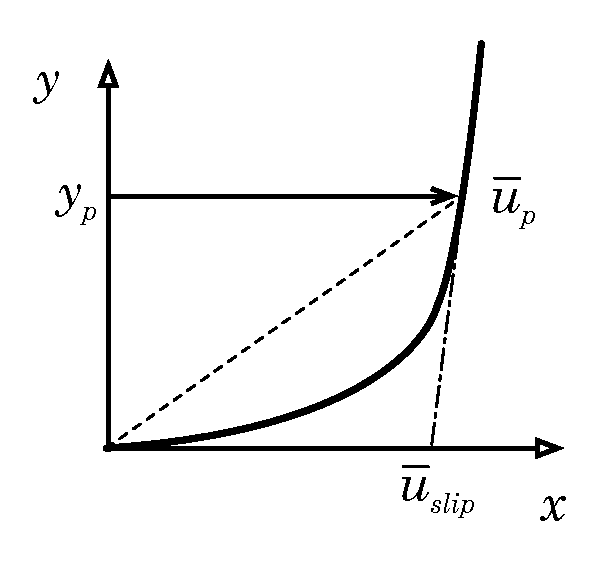
\includegraphics[width=5cm,clip]{wallfunc.eps}
\end{center}
\caption{壁面近傍の無次元速度プロファイル(\cite{kajishima:99:simulation}から転写)}
\label{fig:wall func}
\end{figure}


%%
\subsubsection{壁法則の適用}
%
\paragraph{発達した流れの場合}
チャネル流や円管内の発達流の場合,平均圧力勾配$\partial p^{\prime} / \partial x_i^{\prime}$と壁面摩擦力$\tau^{\prime}_w$が釣り合うので,\textbf{式(\ref{eq:friction velocity})}から摩擦速度がわかる.
第一格子点が対数則の範囲内であることが確認できれば,\textbf{式(\ref{eq:log-law log_e})}を利用できる.

%
\paragraph{流れの状況に応じて壁面摩擦が決まる場合}
一般的には,流れの様子により局所的な摩擦速度の大きさは異なるため,反復的に求める.
ある時点での$y_p^{\prime}$における$u_p^{\prime}$を与えて,関数として次の形を満たす$u_{\tau}^{\prime}$をニュートン反復により求める.

\begin{equation}
F(u_{\tau}^{\prime}) \,\equiv \, \frac{u_p^{\prime}}{u_{\tau}^{\prime}} - \frac{1}{\kappa}\mathrm{ln}\,\left( \frac{u_{\tau}^{\prime} \, y_p^{\prime}}{\nu} \right)\,-\,C \,=\,0
\label{eq:wall func newton}
\end{equation}

\noindent mを反復回数とすると,
\begin{equation}
{u_{\tau}^{\prime}}^{m+1} \,=\, {u_{\tau}^{\prime}}^{m} - \frac{F\left( {u_{\tau}^{\prime}}^{m} \right)}{F^{(1)} \left( {u_{\tau}^{\prime}}^{m} \right)}
\label{eq:newton iteration wall func}
\end{equation}

\noindent 対数則の場合には$F$の一階導関数は,
\begin{equation}
F^{(1)} \left( {u_{\tau}^{\prime}} \right) \,=\,
- \left( {\frac{u_p^{\prime}}{u_{\tau}^{\prime}} + \frac{1}{\kappa}} \right) \, \frac{1}{u_{\tau}^{\prime}}
\label{eq:derivative wall func}
\end{equation}

\noindent \textbf{式(\ref{eq:wall func newton})}$\sim$\textbf{(\ref{eq:derivative wall func})}から反復式を表すと,

\begin{equation} 
{u_{\tau}^{\prime}}^{\,m+1} \,=\, {u_{\tau}^{\prime}}^{\,m} + 
\frac{ 
\displaystyle{
\left\{
\frac{u_p^{\prime}}{{u_{\tau}^{\prime}}^{\,m}}
 - \frac{1}{\kappa} \, 
 \mathrm{ln}\,\left( \frac{y_p^{\prime} \, {u_{\tau}^{\prime}}^{\,m}} {\nu} \right) 
 \,-\, C \right\} \, 
 {u_{\tau}^{\prime}}^{\,m} }
}
{ \displaystyle{ \frac{u_p^{\prime}}{{u_{\tau}^{\prime}}^{\,m}} + \frac{1}{\kappa} }
}
\label{eq:newton iteration wall func}
\end{equation}


摩擦速度を無次元で表し$u_{\tau}\,=\,u_{\tau}^{\prime}/u_0^{\prime}$とすると,

\begin{equation} 
u_{\tau}^{\,m+1}
\, = \,
u_{\tau}^{\,m} + 
\frac{ 
\displaystyle{
\left\{ 
u_p^{+\,m} - \frac{1}{\kappa} \, 
 \mathrm{ln}\,\left( y_p^{+\,m} \right) \,-\, C \right\} \, u_{\tau}^{\,m} }
}
{ \displaystyle{ u_p^{+\,m} + \frac{1}{\kappa} }
}
\label{eq:newton iteration wall func ND}
\end{equation}

上記の手順により求めた$u_{\tau}^{\prime}$に対して,$y_p^{\prime}$が対数則の範囲にあるかどうかを判定し,壁法則を適用する.

%
\vspace{5mm}
\paragraph{摩擦速度求解のアルゴリズム}
与えられたセル近傍の速度から摩擦速度を求める手順は以下のようになる.

\begin{enumerate}
\item 反復の初期値を計算する.
\begin{equation}
\begin{array}{l}
\vspace{3mm}
\displaystyle{ \tau_w^0 \,=\, \frac{\tau_w^{\,\prime}}{\rho^{\prime} {u_0^{\prime}}^2} \,=\, \frac{1}{Re} \frac{\partial u}{\partial y} }\\
\vspace{3mm}
\displaystyle{ u_{\tau}^{\,0} \,=\, \frac{u_{\tau}^{\prime\,0}}{u_0^{\prime}} \,=\, \frac{1}{u_0^{\prime}} \sqrt{\frac{\tau_w^{\,\prime}}{\rho^{\prime}}}
\,=\, \sqrt{\frac{1}{Re} \frac{\partial u}{\partial y}} }\\
\vspace{3mm}
\displaystyle{ {y_p^+}^{\,0} \,=\, \frac{u_{\tau}^{\,0} \, u_0^{\prime} \, y_p^{\prime} }{\nu} }
\,=\, u_{\tau}^{\,0} \, y_p^{\prime} \, \frac{Re}{L^{\prime}}\\
\end{array}
\label{eq:initial iteration fric vel}
\end{equation}
ここで,$L^{\prime}$は代表長さ,$y_p^{\prime}=h^{\prime}/2$(バイナリボクセルの場合は,壁面から半セルの距離)である.
速度勾配は次の2つの候補がある.
\vspace{1mm}

\begin{indentation}{5zw}{0zw}

\begin{enumerate}
\item 壁面から半セルの距離にある速度定義点の速度の大きさで評価
\begin{equation}
\frac{\partial u}{\partial y}  \,=\, \frac{\Delta u}{\Delta y} \,=\, \frac{|u|}{h/2}
\label{eq:vel mag wall func}
\end{equation}

\item \textbf{図\ref{fig:wall func}}の$y_p$の位置での速度勾配を壁関数\textbf{(\ref{eq:log-law log_10})}から求める
\begin{equation}
\frac{\partial u}{\partial y}  \,=\, \frac{5.75}{y_p^+ \, \mathrm{ln}10}
\label{eq:dudy wall func}
\end{equation}

\end{enumerate}

\end{indentation}

\vspace{2mm}

\item Newton反復(常用対数を用いて)
\begin{equation} 
u_{\tau}^{\,m+1} \,=\, u_{\tau}^{\,m} + 
\frac{ \displaystyle{
\left\{ u_p^{+\,m} -  5.75 \, \mathrm{log_{10}}\,{y_p^+}^m \,-\, 5.5 \right\} \, u_{\tau}^{\,m} }
}{ \displaystyle{
u_p^{+\,m} + \frac{1}{\kappa} }
}
\label{eq:newton iteration wall func ND2}
\end{equation}

\vspace{2mm}
\item 収束判定
次式により収束判定を行う.
\begin{equation} 
\displaystyle{ \frac{|u_{\tau}^{\,m+1}-u_{\tau}^{\,m}|}{|u_{\tau}^{\,m}|} < \epsilon_2 \quad(=10^{-3}) }
\label{eq:newton iteration criteria}
\end{equation}

ここで,$u_{\tau}^{\,m+1}<\epsilon_2$の場合には,安定性のために$u_{\tau}^{\,m+1}=\epsilon_2$とする.
\vspace{2mm}

\item 更新\\
\begin{equation}
\begin{array}{l}
u_{\tau}^{\,m} \,=\, u_{\tau}^{\,m+1}\\
\vspace{2mm}
\displaystyle{ {y_p^+}^{\,m} \,=\, u_{\tau}^{\,m+1} \, y_p^{\prime} \, \frac{Re}{L^{\prime}} }\\
\end{array}
\label{eq:newton iteration wall func ND2}
\end{equation}
\vspace{2mm}

\item 上記を収束するまで繰り返す.反復上限を10回程度で抑えておく.
\end{enumerate}


%
\subsubsection{減衰関数を用いたすべりなし条件}

壁近傍ではGSで速度勾配があるため,SGS応力が生じる.しかし,壁面上では$\tau_{ij}=0$なので,これを打ち消す必要がある.
Smagorinskyモデルでは減衰関数$f_s$を導入し,渦粘性係数を補正する.

\begin{equation}
\nu_e \,=\, \left( Cs \,f_s \, \overline{\Delta} \right)^2 \left| \overline{D} \right|
\label{eq:nu-SGS modified}
\end{equation}

\noindent 減衰関数としてはvan Driest関数を用いる.

\begin{equation}
f_s \,=\, 1 - \mathrm{exp} \left( -\frac{y^+}{A^+} \right)
\label{eq:van-driest}
\end{equation}

\noindent $A^+$は無次元の定数で約25が用いられる.

すべりなし条件を用いる場合には,粘性底層からバッファ層にかけて,格子点が数点必要である.
この場合,粘性底層内では乱流応力は無視できるので,壁面摩擦応力$\tau_w^{\prime}$は次のように決められる.

\begin{equation}
\tau_w^{\prime} \,=\, \mu \left| \frac{\partial \overline{u^{\prime}}}{\partial y^{\prime}} \right|_{wall}
\label{eq:viscous layer stress}
\end{equation}

%
\subsection{壁法則から求めた壁面摩擦応力による粘性応力の置換}
壁面に接する流体セルの固体セルへの接平面上の壁面摩擦応力$\tau_w^{\prime}=\mu(\partial u^{\prime}/\partial y^{\prime})$は壁法則\textbf{(\ref{eq:friction velocity})}から求められる摩擦速度から$\tau_w^{\prime}\,=\, \rho^{\prime} {u_{\tau}^{\prime}}^2$として計算される.この壁面摩擦応力を粘性項の離散式に代入し境界条件とする.たとえば,z軸のマイナス方向に壁面がある場合,無次元形式で,

\begin{equation}
\frac{1}{Re} \frac{\partial}{\partial z} \left( \frac{\partial u}{\partial z} \right)
\,=\,
\frac{1}{h} \, \left( {\frac{1}{Re} \frac{\partial u}{\partial z}_t - \tau_{w,\,b} } \right)
\label{eq:replace wall shear stress}
\end{equation}


計算された摩擦速度から壁面摩擦応力を計算し,\textbf{式(\ref{eq:replace wall shear stress})}により境界条件を与える.固体セルに隣接する流体セルにおいて摩擦速度が求まると,固体に接する面上の応力は次式により計算される.

\begin{equation} 
\tau_w\,=\, u_{\tau}^2
\label{eq:wall stress from fric vel}
\end{equation}

\noindent しかしながら,複数の固体面に接するセルでは各方向同じ大きさの壁面摩擦応力となるし,軸方向に沿わない速度ベクトルの場合には過大評価になる可能性がある.そこで,速度ベクトルの方向成分を計算し,各方向へ射影する.つまり,\textbf{式(\ref{eq:wall stress from fric vel})}に用いる$u_{\tau}$を再定義する.

\begin{equation} 
\tau_{w,\,i} \,=\, {\left( u_{\tau} \frac{u_i}{|u|} \right)}^2
\label{eq:redefine of friction velocity}
\end{equation}





%
\chapter{EBCスキームと境界条件処理}
\label{chpt:ebcs}
\begin{abstract}
この章では,直交 Euler 格子のコロケート変数配置の場合に,任意位置の境界条件を効率よく処理する方法として,スキーム中に境界条件を実装方法について述べる.
\end{abstract}
\graphicspath{{./fig_EBCS/}}
%
\section{Embedded Boundary Condition Scheme}

\hypertarget{tgt:ebcs}{Embedded Boundary Condition Scheme}は,直交格子で任意形状を扱うために境界条件をスキーム中に埋め込む方法の総称とする.
物体の形状近似の程度によってその実装は異なる.
最も簡単な物体表現としては,物体を0と1(マスク情報)で表現するBinary近似,つまりレゴブロックのような物体形状がある.
この場合には,マスク情報を使って必要な評価点での流束などを計算できるようにスキームを実装する.
形状近似度を改善する場合,格子に沿わない方向の物体形状の影響を取り込めるように,スキームを構築する方法がある.
セル内を平面で近似する方法や曲面近似など様々なバリエーションが考えられる.
古典的なカットセルはこの範囲になる.

本章では,バイナリ近似と面近似の実装について述べる.

%%%
\section{Binary近似の解法}

計算領域における任意の位置における境界条件をバイナリ近似の基に統一的に処理するために,\textbf{式(\ref{eq:mask function})}に示すフラグ$\phi$を用いた線形結合により\textbf{式(\ref{eq:ebcs_flagging})}のように離散式を表現する.

\begin{equation}
\phi \,=\, \left\{
\begin{array}{ll}
0 & \mathrm{Non-fluid\, cell}\\
1 & \mathrm{Fluid\, cell}\\
\end{array} \right.
\label{eq:mask function}
\end{equation}

\begin{equation}
p \,=\, p\, \phi + (1-\phi)\, p^{\,BC}
\label{eq:ebcs_flagging}
\end{equation}

\noindent 上式は,$\phi=1$のとき本来の値$p$になり,$\phi=0$のときに指定する境界条件の値$p^{\,BC}$になる.基本的にはif文でも記述できるが,パイプラインの効率的な動作を期待した実装を行う.

%
\subsection{圧力のPoisson方程式}
非圧縮コードのホットスポットの一つは\hypertarget{tgt:Poisson Binary}{圧力のPoisson方程式}の反復部分であるため,この反復部分を効率よく計算したい.そのためには,収束性の高い反復解法の選択,効率的な反復法の実装が必要になる.ここでは後者の実装について,メモリと実行性能の点を検討する.

近年の計算機アーキテクチャは,階層的なメモリ構造,パイプライン演算器,キャッシュ構造などのハードウェア構成により,SIMD命令の有効利用が高性能計算に必要になる.高性能計算に必要なことは,プロセッサへデータを連続的に供給し,かつ取り出すことである.そのためにはメモリからプロセッサへのデータ転送能力が重要な鍵となる.
反復解法ではメモリからのデータ供給と演算数の比(Byte/Flop値)が実効性能に大きく影響する.特に,構造格子上の差分法ではB/F=$2\sim5$程度となるだろう.B/F値をできるだけ小さく抑えるためには,メモリからのロードストア数を減らすことが必要である.

一方,実用コードの特徴的な点として,多様な境界条件に対応することが要求される.このため,境界条件を含んだ反復解法部分の高速処理を考える必要がある.
これらの点を考慮して,次のポリシーにより反復解法部分を設計する.

\begin{enumerate}
\item EBCSによる境界条件を含んだ統一的な反復式の表現.
\item ロードの抑制のため,必要な係数をビットにエンコードする.
\item ライブラリを含む反復解法を選択可能なように反復解法クラスを設計する.
\end{enumerate}

%
\subsubsection{圧力境界条件の種類}
圧力の境界条件の分類として,次の2通りがある.
\begin{enumerate}
\item 数学的な分類
Neumann型条件とDirichlet型条件
\item 物理的な分類
計算内部領域の境界条件と外部境界条件
\end{enumerate}

数学的な分類の観点からは,次のような状況が考えられる.

\begin{itemize}
\item \hypertarget{tgt:EBCS poisson BC}{Neumann条件}
\begin{itemize}
\item 勾配値が不変の場合\\
$\nabla p = const.$を反復ループの外側で与える.\vspace{1mm}
\item 勾配値がタイムステップ間では一定であるが,時間的には変化する場合\\
勾配値を反復ループの外側で与える.\vspace{1mm}
\item 勾配値が反復毎に変化する場合\\
勾配値がNavier-Stokes方程式から計算される場合で,壁面境界条件,流入条件などに用いる.\vspace{1mm}
\end{itemize}

\item Dirichlet条件
\begin{itemize}
\item 値が不変の場合\\
値を反復ループの外側で与える.\vspace{1mm}
\item 値がタイムステップ間では一定であるが,時間的には変化する場合\\
値を反復ループの外側で与える.\vspace{1mm}
\end{itemize}
\end{itemize}



%
\subsubsection{EBCSによるPoisson反復離散式の表現}
連続の式と Fractional Step法のポテンシャルの修正式から導かれる圧力の Poisson 方程式は\textbf{式(\ref{eq:Poisson_from_FS})}のようになる.

\begin{equation}
\nabla \left( \nabla p^{\,n+1} \right) \,=\, \frac{1}{\Delta t} div\, (u^{\,*}) \equiv \psi
\label{eq:Poisson_from_FS}
\end{equation}

反復式に組み込む境界条件とパターンして,以下の3種類を考慮する.

\begin{enumerate}
\item Dirichlet条件
\begin{equation}
p \,=\, p^{\,BC}
\label{eq:dirichlet bc in poisson}
\end{equation}

外部境界条件での利用を想定している.\\

\item Neumann条件
\begin{equation}
\nabla p \,=\, \left \{
\begin{array}{ll}
\nabla p^{\,BC} & 1\, \mathrm{time\, step}中で一定値をとり,圧力\mathrm{Poisson}の反復過程で固定値となる.\\
f(u_{\,i}) & \mathrm{NS}式から圧力勾配項を計算するので,反復毎に値が変化する.
\end{array} \right .
\label{eq:neumann bc in poisson}
\end{equation}

\item 固体中の圧力\\
固体中の圧力はマスクなどによりゼロとして扱うと,圧力がドリフトした場合にゼロ固定で残るため,結果を見る場合に誤解を招いたり,描画処理で不都合がある.そこで,周囲の値の範囲内に自然に収まるように,ラプラス方程式\textbf{(\ref{eq:laplace_eq})}を解く.
\begin{equation}
\nabla \left( \nabla p^{\,n+1} \right) \,=\, 0
\label{eq:laplace_eq}
\end{equation}
\end{enumerate}

\vspace{5mm}

%
\begin{indentation}{3zw}{0zw}
\paragraph{Neumann条件の導入} $\mbox{}$\\
 EBCSを用いて,\textbf{式(\ref{eq:Poisson_from_FS})}にNeumann条件を導入すると,

\begin{equation}
\begin{array}{lll}
\vspace{2mm}
\nabla \left( \nabla p \right) \,=\, \psi \quad \rightarrow & \displaystyle { \frac{1}{h} \, \{ }
&   {\left( \nabla p \,\phi^{\,N} \right)}_{\,e} + \left( 1-\phi^{\,N}_e \right) \,\nabla p^{\,BC}_e 
  - {\left( \nabla p \,\phi^{\,N} \right)}_{\,w} - \left( 1-\phi^{\,N}_w \right) \,\nabla p^{\,BC}_w \\
\vspace{2mm}
&+& \displaystyle{ {\left( \nabla p \,\phi^{\,N} \right)}_{\,n} + \left( 1-\phi^{\,N}_n \right) \,\nabla p^{\,BC}_n 
  - {\left( \nabla p \,\phi^{\,N} \right)}_{\,s} - \left( 1-\phi^{\,N}_s \right) \,\nabla p^{\,BC}_s } \\
\vspace{2mm}
&+& \displaystyle{ {\left( \nabla p \,\phi^{\,N} \right)}_{\,t} + \left( 1-\phi^{\,N}_t \right) \,\nabla p^{\,BC}_t 
  - {\left( \nabla p \,\phi^{\,N} \right)}_{\,b} - \left( 1-\phi^{\,N}_b \right) \,\nabla p^{\,BC}_b \quad \} = \psi } 
\end{array}
\label{eq:ebcs_neumann}
\end{equation}

\noindent ここで$\phi^{\,N}_{\,l}$は,Neumann条件を表すセルフェイスの境界条件マスクで,三次元の場合,1つのセルに対して6方向$l=\{e,w,n,s,t,b\}$存在し,\textbf{式(\ref{eq:neumann_bc_mask})}の値をとる.

\begin{equation}
\phi^{\,N}_l \, = \, \left\{
\begin{array}{ll}
1 & \mathrm{Normal\,face\,in\,a\,fluid\,cell}\\
0 & \mathrm{Neumann\,boundary\,face}
\end{array} \right. 
\label{eq:neumann_bc_mask}
\end{equation}

\textbf{式(\ref{eq:ebcs_neumann})}を整理して,境界条件部分を右辺項に移動すると,

\begin{equation}
\frac{1}{h} \left \{ \,
  {\left( \nabla p \,\phi^{\,N} \right)}_{\,e} - {\left( \nabla p \,\phi^{\,N} \right)}_{\,w} 
+ {\left( \nabla p \,\phi^{\,N} \right)}_{\,n} - {\left( \nabla p \,\phi^{\,N} \right)}_{\,s} 
+ {\left( \nabla p \,\phi^{\,N} \right)}_{\,t} - {\left( \nabla p \,\phi^{\,N} \right)}_{\,b} \, \right \} \,=\, \psi
\label{eq:ebcs_poisson2}
\end{equation}

\begin{equation}
\sum \limits_l {\left( \nabla p \,\phi^{\,N} \right)}_{\,l} \,n_{\,l}
\,=\, h\,\psi \,-\, \sum \limits_l \left( 1-\phi^{\,N}_{\,l} \right) \,\nabla p^{\,BC}_{\,l} \,n_{\,l}
\label{eq:ebcs_poisson4}
\end{equation}

\noindent Volterraの原理\index{Volterra}を用いて半離散的に表し\footnote{表記はベクトルで,添え字はセル界面の番号であることに注意する~\cite[p.~39]{nakamura:98:handbook}.},$l$は隣接セルフェイスの意味で$l=\{e,w,n,s,t,b\}$,$n_{\,l}$はセルの外側方向の単位法線とする.$\phi$はセルフェイスで定義された値であるが,$p$についてはその方向の隣のセルの値を意味する.

%
\paragraph{Dirichlet条件の導入} $\mbox{}$\\
 次に,Dirichlet条件を組み込む.\textbf{式(\ref{eq:neumann_bc_mask})}と同様に,Dirichlet条件を表すセルフェイスの境界条件マスクを次式で表す.

\begin{equation}
\phi^{\,D}_l \, = \, \left\{
\begin{array}{ll}
1 & \mathrm{Normal\,face\,in\,a\,fluid\,cell}\\
0 & \mathrm{Dirichlet\,boundary\,face}
\end{array} \right. 
\label{eq:dirichlet_bc_mask}
\end{equation}

\noindent セルを構成する面に対しては,一つの面についてNeumann条件かDirichlet条件のどちらか一方しか指定できないので,両者は排他的である点に注意する.EBCSを用いて\textbf{式(\ref{eq:ebcs_poisson4})}左辺の各勾配項にDirichlet条件のフラグ\textbf{(\ref{eq:dirichlet_bc_mask})}を導入する.

\begin{equation}
\left .
\begin{array}{lll}
\vspace{1mm}
{\left( \nabla p \,\phi^{\,N} \right)}_{\,e} &=& \displaystyle{ \frac{1}{h}\left\{\,p_{\,i+1}\,\phi^{\,D}_{\,e} \,+\, \left(1-\phi^{\,D}_{\,e}\right)\,p^{\,BC}_{\,e} - p_{\,i} \,\right \} \phi^{\,N}_{\,e} } \\
\vspace{1mm}
{\left( \nabla p \,\phi^{\,N} \right)}_{\,n} &=& \displaystyle{ \frac{1}{h}\left\{\,p_{\,j+1}\,\phi^{\,D}_{\,n} \,+\, \left(1-\phi^{\,D}_{\,n}\right)\,p^{\,BC}_{\,n} - p_{\,j} \,\right \} \phi^{\,N}_{\,n} } \\
\vspace{1mm}
{\left( \nabla p \,\phi^{\,N} \right)}_{\,t} &=& \displaystyle{ \frac{1}{h}\left\{\,p_{\,k+1}\,\phi^{\,D}_{\,t} \,+\, \left(1-\phi^{\,D}_{\,t}\right)\,p^{\,BC}_{\,t} - p_{\,k} \,\right \} \phi^{\,N}_{\,t} } \\
\vspace{1mm}
{\left( \nabla p \,\phi^{\,N} \right)}_{\,w} &=& \displaystyle{ \frac{1}{h}\left\{\,p_{\,i} - p_{\,i-1}\,\phi^{\,D}_{\,w} \,-\, \left(1-\phi^{\,D}_{\,w} \right)\,p^{\,BC}_{\,w} \,\right \} \phi^{\,N}_{\,w} } \\
\vspace{1mm}
{\left( \nabla p \,\phi^{\,N} \right)}_{\,s} &=& \displaystyle{ \frac{1}{h}\left\{\,p_{\,j} - p_{\,j-1}\,\phi^{\,D}_{\,s} \,-\, \left(1-\phi^{\,D}_{\,s} \right)\,p^{\,BC}_{\,s} \,\right \} \phi^{\,N}_{\,s} } \\
\vspace{1mm}
{\left( \nabla p \,\phi^{\,N} \right)}_{\,b} &=& \displaystyle{ \frac{1}{h}\left\{\,p_{\,k} - p_{\,k-1}\,\phi^{\,D}_{\,b} \,-\, \left(1-\phi^{\,D}_{\,b} \right)\,p^{\,BC}_{\,b} \,\right \} \phi^{\,N}_{\,b} } \\
\end{array} \quad \right \}
\label{eq:ebcs_dirichlet}
\end{equation}

\vspace{5mm}
\textbf{式(\ref{eq:ebcs_poisson4})}と\textbf{式(\ref{eq:ebcs_dirichlet})}をまとめると,

\begin{equation}
\sum \limits_l {\left( p \,\phi^{\,D} \,\phi^{\,N} \right)}_{\,l} \,-\, p \sum \limits_l \phi^{\,N}_{\,l}
\,=\,
\underbrace{h^2 \,\psi} \limits_{\gamma^{\,0}}
\,-\, 
\underbrace{ h \sum \limits_l \left( 1-\phi^{\,N}_{\,l} \right) \,\nabla p^{\,BC}_{\,l} \,n_{\,l} } \limits_{\gamma^{\,N}}
\,-\, 
\underbrace{ \sum \limits_l \left(1-\phi^{\,D}_{\,l} \right) \,p^{\,BC}_{\,l} \phi^{\,N}_{\,l} \,n_{\,l} } \limits_{\gamma^{\,D}}
\label{eq:ebcs_poisson3}
\end{equation}

\noindent 右辺第一項目$\gamma^{\,0}$は連続条件と速度境界条件に由来する項である.第二項目はNeumann条件$\gamma^{\,N}$,第三項目はDirichlet条件$\gamma^{\,D}$の寄与である.更に,Dirichlet, Neumann条件を反復間で固定値をとる$\gamma^{\,D1},\,\gamma^{\,N1}$と,反復毎に値が変わる$\gamma^{\,D2},\,\gamma^{\,N2}$に分ける.\textbf{式(\ref{eq:ebcs_poisson3})}右辺のソース項の種類を\textbf{表\ref{tbl:BC of pressure}}に分類して示す.
$p^{\,BC}_{\,l}$は仮想的に与える圧力値であることに注意する.つまり,計算空間のセルには直接値を代入しない.

反復回数を$k$としてSOR法系の反復式を構成すると,

\begin{equation}
\left.
\begin{array}{lll}
\vspace{2mm}
\tilde{p} & = & \displaystyle { \frac{1}{\sum \limits_l \left( \, \phi^{\,N}_{\,l} \, \right)} 
\left \{ \,
\sum \limits_l {\left( p \,\phi^{\,D} \,\phi^{\,N}\right)}_{\,l} 
\underbrace{ \,-\, \gamma^{\,0} \,+\, \gamma^{\,D1} \,+\, \gamma^{\,N1} } \limits_{反復中固定値}
\underbrace{ \,+\, \gamma^{\,D2} \,+\, \gamma^{\,N2} } \limits_{反復毎に変化}
\, \right \} } \\
\vspace{2mm}
\Delta p & = & \tilde{p} \,-\, p^{\,k} \\
\vspace{5mm}
p^{\,k+1} & = & p^{\,k} \,+\, \omega\, \,\Delta p \\

\vspace{2mm}
\gamma^{\,0} & = & h^2 \,\psi \\
\vspace{2mm}
\gamma^{\,D^1} & = & \sum \limits_l \left(1-\phi^{\,D}_{\,l} \right) \,p^{\,BC}_{\,l} \phi^{\,N}_{\,l} \,n_{\,l} \\
\vspace{2mm}
\gamma^{\,D^2} & = & \sum \limits_l \left(1-\phi^{\,D}_{\,l} \right) \,p^{\,BC}_{\,l} \phi^{\,N}_{\,l} \,n_{\,l} \\
\vspace{2mm}
\gamma^{\,N^1} & = & h \sum \limits_l \left( 1-\phi^{\,N}_{\,l} \right) \,\nabla p^{\,BC}_{\,l} \,n_{\,l} \\
\vspace{2mm}
\gamma^{\,N^2} & = & h \sum \limits_l \left( 1-\phi^{\,N}_{\,l} \right) \,\nabla p^{\,BC}_{\,l} \,n_{\,l} \\

\end{array} \qquad \right \}
\label{eq:poisson_iteration}
\end{equation}

\noindent 上式は,Neumann条件とDirichlet条件を含む圧力反復式で,流体セルと固体セルに適用する.ここで問題点は,周囲を壁で囲まれた孤立した流体セルの場合,対角項の係数がゼロとなる場合である.そのようなセルでは流れは生じないので強制的に固体壁にして,少なくとも1面は流体セルと接することを保証する\footnote{処理としては,壁面と流入出条件に由来する全てのNeumannBCフラグをセットした後,全周NeumannBCフラグのセルをみつけ,状態を変更する.}.

\textbf{表\ref{tbl:BC of pressure}}に示す壁面条件については,圧力勾配の評価方法に2種類ある.$\nabla p=0$は高レイノルズ数の場合に用いられる近似的な圧力境界条件であり,もう一方は低レイノルズ数の場合などに用いる厳密な境界条件である.後者の方がよい近似であるが,計算コストは高い.
壁面条件の評価方法は,Steerセクション内の\verb|Pressure_BC_for_wall_surface|タグで指定する\footnote{Pressure\_BC\_for\_wall\_surface = grad\_zero or grad\_NS}.

Neumann条件とDirichlet条件で値がゼロの場合には,ソース項の計算は簡単になる.つまり,内部境界,外部境界ともに$\gamma^{\,N1},\,\gamma^{\,D}$については計算不要となり,$\gamma^{\,N2}$のみを計算すればよい\footnote{境界条件のビットフラグ$\phi^{\,D},\,\phi^{\,N}=1$で有効な場合でもその値がゼロであるから.}.したがって,\textbf{表\ref{tbl:BC of pressure}}の境界条件に対して,固定ソース項は速度境界条件による$\gamma^{\,0}$のみを考慮すればよい.

\begin{table}[htdp]
\small
\caption{内部と外部境界に指定できる圧力境界条件の種類}
\begin{center}
\begin{tabular}{l|ccl|l} \toprule
境界条件の種類 & 内部 & 外部 & ソース項 & 実装\\ \midrule
壁面境界 $\nabla p=0$ & ○ & ○ & $\gamma^{\,N1}$ & $\partial p/\partial x_i =0$\\
     $\nabla p=f(u_i)$ & ○ & ○ & $\gamma^{\,N2}$ & $\partial p/\partial x_i =  1/Re (\partial^2 u_i/\partial x_i^2)$\\
対称境界 $\nabla p=0$ & - & ○ & $\gamma^{\,N1}$ & $\partial p/\partial x_i =0$\\
流入境界 $\nabla p=f(u_i)$ & ○ & ○ & $\gamma^{\,N2}$ & $\partial p/\partial x_i = - \partial u_i / \partial t -(u_j-u_j^{\,g}) (\partial u_i / \partial x_j) + 1/Re (\partial^2 u_i/\partial x_i^2)$\\
流出境界 $\nabla p=0$ & ○ & ○ & $\gamma^{\,N1}$ & $\partial p/\partial x_i =0$\\
     $p=0$ & ○ & ○ & $\gamma^{\,D}$ & \\
遠方境界 $p=0$ & - & ○ & $\gamma^{\,D}$ & トラクションフリー\\
流入出境界 & - & ○ & -  & 流出境界と,(流入として)遠方境界の切り替え\\
周期境界 & - & ○ & - & データコピー\\ 
周期境界 & - & ○ & $\gamma^{\,D^2}$ & ドライバ\\ \bottomrule
\end{tabular}
\end{center}
\label{tbl:BC of pressure}
\end{table}

%
\paragraph{Dirichlet境界条件の利用}
Dirichlet型の境界条件は,計算外部領域であるガイドセルに与える場合を想定している.
ガイドセル上に指定される場合には,そのセルは計算せず,単に参照値として利用されるのみである.
具体的には,遠方境界と流入出境界条件の場合の流入時(トラクションフリー)には$p=0$を利用する.
この場合は,外部境界を含む計算内部セルの該当面にDirichlet BCフラグをゼロにセットして計算する.

%
\paragraph{内部境界条件と外部境界条件の取り扱い}
\textbf{表\ref{tbl:BC of pressure}}に示すように,内部境界条件と外部境界条件は$\partial p/\partial x_i = 0$や$p=0$など比較的簡単な形式である.計算時には内部と外部を区別せずに,ビットフラグの状況によりソース項の計算の後,\textbf{式(\ref{eq:poisson_iteration})}を計算する実装としている.ただし,周期境界条件のみは,反復後に処理する.

%
\paragraph{固体セルの場合のPoisson反復}
固体セルの場合には,前述のようにラプラス方程式を解き,値が平滑化され周囲の値の平均値となることを期待する.
この場合,求まった固体中の圧力には物理的な意味はない.
Laplace方程式を解く場合,\textbf{図\ref{fig:N&D bit flag}}において,Sセルは全ての面で$\phi^{\,N}=1$を与え,\textbf{式(\ref{eq:poisson_iteration})}において$\psi=0$として反復する.

固体中の圧力も解くことになるので,収束ノルムをL2とする場合には,固体セルの残差もノルム評価に加えられる点に注意する.流体を1セルの固体セルで分離しているような状況で,固体セルの両側の流体セルで圧力値が大きく異なる場合には,固体セルの圧力勾配が大きくなり,収束性が悪くなることもあり得る.一方,ノルムに$div\,(\boldmath{u}^{\,n+1})$をとる場合には,収束性は流体のみを解いている場合と変わりない(はず..).

%
\paragraph{圧力境界条件に利用するビットフラグ}
セルの面の状態を表すNeumann条件\textbf{(\ref{eq:neumann_bc_mask})}やDirichlet条件\textbf{(\ref{eq:dirichlet_bc_mask})}のフラグを効率的に実装するため,フラグを1bitで表現し,整数型の変数にまとめて保持する.ビット操作による演算コストは,フラグを通常の変数で保持しロードするコストに比べれば少ない.4バイト整数へのビットの割り当てを\textbf{表\ref{tbl:Flags in bcd}},\textbf{表\ref{tbl:Flags in bcp}}に示す.

\textbf{図\ref{fig:N&D bit flag}}に示すように,通常の流体セル(F)と固体セル(S)を考える.Neumann条件とDirichlet条件をフラグにより各フェイスに与え,\textbf{式(\ref{eq:ebcs_poisson3})}を計算する.

\begin{figure}[htbp]
\begin{center}
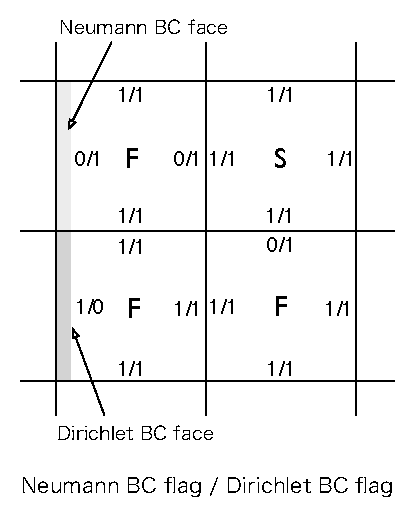
\includegraphics[width=5.5cm,clip]{bit_flag_P.eps}
\end{center}
\caption{圧力反復式に用いるビットフラグ.各セルについて,6つのフラグ(三次元の場合)を設定する.Sセルは固体セル,Fセルは通常の流体セルであり,この例では,左下のセルにDirichlet境界,左上のセルにNeumann境界が与えられている.Neumann BCフラグは,Neumann条件が与えられたセル面と固体セルに接する流体セルの接触面をゼロに設定する.}
\label{fig:N&D bit flag}
\end{figure}


%
\paragraph{連立一次方程式の係数行列と定数ベクトルの計算}
\textbf{式(\ref{eq:ebcs_poisson3})}を離散化して得られる連立一次方程式$\mathrm{A}\,\bm{x}=\bm{b}$の係数行列$\mathrm{A}$と定数ベクトル$\bm{b}$については,前述したポリシーから以下のようにまとめられる.

\begin{itemize}
\item ビットフラグの計算\\
エンコードして保持しておくフラグは,次の4種類である.
\begin{equation}
\small
\left.
\begin{array}{lll}
\vspace{2mm}
\displaystyle{ \phi^{\,D}_{\,l}\, \phi^{\,N}_{\,l} } & 6方向\,\times\,1\,\mathrm{bit}\quad (6\,\mathrm{bits}) & \mathrm{ BC\_NDAG\_\{E,W,N,S,T,B\} } \\
\vspace{2mm}
\displaystyle{ \phi^{\,N}_{\,l} } & 6方向\,\times\,1\,\mathrm{bit}\quad (6\,\mathrm{bits}) & \mathrm{ BC\_N\_\{E,W,N,S,T,B\} }\\
\vspace{2mm}
\displaystyle{ \phi^{\,D}_{\,l} } & 6方向\,\times\,1\,\mathrm{bit}\quad (6\,\mathrm{bits}) & \mathrm{ BC\_D\_\{E,W,N,S,T,B\} }\\
\vspace{2mm}
\displaystyle{ \sum \limits_l \left( \, \phi^{\,N}_{\,l} \, \right) } & 1 \sim 6 \quad (3\,\mathrm{bits}) & \mathrm{ BC\_DIAG }\\
\end{array} \quad \right\}
\label{eq:bit flag}
\end{equation}

\item 定数ベクトルの計算\\
計算内部領域における固体セルを計算する場合,定数項を$\psi=0$と修正する.
\end{itemize}

%
\paragraph{圧力Poisson部の計算手順}
\textbf{式(\ref{eq:ebcs_poisson3})}を\textbf{\ref{eq:poisson_iteration}}の手順で解く場合,ソース項の処理は以下のように考える.

\begin{indentation}{3zw}{0zw}
{ \small
\noindent begin: Time step loop\\
\hspace{1cm}pseudo vectorの計算\\
\hspace{1cm}Poissonのソース項 $\gamma^{\,0}$の計算\\
\hspace{1cm}Poissonのソース項 $\gamma^{\,N1}$の計算(反復中に変化しない条件:壁面,対称,流出)\\
\hspace{1cm}Poissonのソース項 $\gamma^{\,D}$の計算(流出,遠方,流入出)\\
\hspace{1cm}begin: Iteration loop\\
\hspace{2cm}Poissonのソース項 $\gamma^{\,N2}$の計算(反復中に変化する条件:壁面,流入)\\
\hspace{2cm}Poissonの求解(\textbf{式\ref{eq:poisson_iteration}})\\
\hspace{1cm}end: Iteration loop\\
end: Time step loop\\
}
\end{indentation}

反復中に変化するNeumann条件は,壁面境界で圧力勾配をNavier-Stokes方程式から求める場合と流入境界の場合である.ソース項の計算タイミングとして,圧力Poissonの反復前と反復内の2通りがある.$\gamma^{\,N1}$は反復前に決まる条件である.一方,壁面境界や流入境界でNS式から圧力勾配を計算する$\gamma^{\,N2}$は反復内で処理する.したがって,ソース項は2つの配列を使って実装している.

\end{indentation}

%
\subsubsection{Fractional Step法における射影ステップの処理}
コロケート変数配置のFractional Step法の計算処理では,セルセンタとセルフェイスに配置された速度ベクトルに対して,\textbf{式(\ref{eq:Pressure correction CC}}, \textbf{\ref{eq:Pressure correction CF})}に示すそれぞれ圧力勾配による射影ステップの計算が必要になる.再掲すると,

\begin{equation}
\left.
\begin{array}{llll}
u_i^{\,n+1} &=& \displaystyle{ u_i^{\,*} - \Delta t {\frac{\partial p}{\partial x_i}}^{n+1} } & \mathrm{(Cell\,center)} \vspace{2mm}\\
u_{i,\,face}^{\,n+1} &=& \displaystyle{ \bar{u}_{i,\,face}^{\,*} - \Delta t {\frac{\partial p}{\partial x_i}}^{n+1} } & \mathrm{(Cell\,face)}\\
\end{array} \qquad \right \}
\label{eq:prj step}
\end{equation}

\textbf{式(\ref{eq:prj step})}の圧力勾配項に対して,\textbf{式(\ref{eq:ebcs_dirichlet})}の圧力勾配の離散式を適用する.

%
\paragraph{セルセンタの圧力勾配}
x方向を例にして,セルセンタの場合の圧力勾配の離散化を示す.

\begin{equation}
\begin{array}{lll}
{\nabla p}_{c,\,x} &=& \displaystyle{ \frac{1}{2} \left( {\nabla p}_e + {\nabla p}_w \right) } \vspace{2mm}\\
 &=& \displaystyle{ \frac{1}{2} \left[
 {\left( \nabla p\,\phi^{\,N} \right)}_e + \left( 1-\phi^{\,N}_e \right) \nabla p^{BC}_e
+{\left( \nabla p\,\phi^{\,N} \right)}_w + \left( 1-\phi^{\,N}_w \right) \nabla p^{BC}_w
 \right] } \vspace{2mm}\\
 &=& \displaystyle{ \frac{1}{2} \left[ \frac{1}{h} \left\{ \phi^{\,D}_e p_{i+1} + \left( 1-\phi^{\,D}_e \right) p^{BC}_{i+1} -p_i \right\} \phi^{\,N}_e + \left( 1-\phi^{\,N}_e \right) \nabla p^{BC}_e \right.} \vspace{2mm}\\
 & & \displaystyle{ \left. + \frac{1}{h} \left\{ p_i - \phi^{\,D}_w p_{i-1} - \left( 1-\phi^{\,D}_w \right) p^{BC}_{i-1} \right\} \phi^{\,N}_w + \left( 1-\phi^{\,N}_w \right) \nabla p^{BC}_w \right]} \vspace{2mm}\\
 &=& \displaystyle{ \underbrace{ \frac{1}{2h} \left\{ \phi^{\,D}_e \phi^{\,N}_e p_{i+1} + \left( \phi^{\,N}_w - \phi^{\,N}_e \right) p_i - \phi^{\,D}_w \phi^{\,N}_w p_{i-1} \right\} }_{(i)} } \vspace{2mm}\\
 & & \displaystyle{ + \underbrace{ \frac{1}{2} \left[
 \frac{1}{h} \left\{ \left( 1-\phi^{\,D}_e \right) \phi^{\,N}_e p^{BC}_{i+1} 
 - \left( 1-\phi^{\,D}_w \right) \phi^{\,N}_w p^{BC}_{i-1} \right\} 
 + \left( 1-\phi^{\,N}_e \right) \nabla p^{BC}_e + \left( 1-\phi^{\,N}_w \right) \nabla p^{BC}_w
 \right] }_{(ii)} } \vspace{2mm}\\
\end{array}
\label{eq:grad p CC}
\end{equation}

\textbf{式(\ref{eq:grad p CC})}において,(i)の項は非境界条件部分の圧力勾配を示す.一方,(ii)の項はDirichlet条件とNeumann条件による圧力勾配を示し,反復ループ外で設定する.
ガイドセルに接しない内部領域は$\nabla p=0$の条件のみなので,(ii)項はゼロとしてよい.
ガイドセルに接する内部領域では,外部境界条件OUTFLOW, TRACTION\_FREEにより$p=0$のDirichlet条件が課せられる場合がある.その場合も参照値がゼロなので,(ii)の評価は不要になる.
$\nabla p=0$の条件を考慮して,\textbf{式(\ref{eq:grad p CC})}を簡潔に表記すると,

\begin{equation}
\begin{array}{lll}
{\nabla p}_{c,\,x}  &=& 
\displaystyle{ \frac{1}{2h} \left\{ \phi^{\,D}_e \phi^{\,N}_e p_{i+1} + \left( \phi^{\,N}_w - \phi^{\,N}_e \right) p_i - \phi^{\,D}_w \phi^{\,N}_w p_{i-1} \right\} }\\
\end{array}
\label{eq:grad p CC 2}
\end{equation}

\paragraph{セルフェイスの圧力勾配}
次に,$i+1$セルがディリクレ境界の場合のセルフェイスの圧力勾配を示す.

\begin{equation}
\begin{array}{lll}
{\nabla p}_{i+1/2,\,x} &=& \displaystyle{ 
 {\left( \nabla p\,\phi^{\,N} \right)}_{i+1/2} + \left( 1-\phi^{\,N}_{i+1/2} \right) \nabla p^{BC}_{i+1/2} } \vspace{2mm}\\
 &=& \displaystyle{ \frac{1}{h} \left\{ \phi^{\,D}_{i+1/2} \, p_{i+1} + \left( 1-\phi^{\,D}_{i+1/2} \right) p^{BC}_{i+1} -p_i \right\} \phi^{\,N}_{i+1/2} + \left( 1-\phi^{\,N}_{i+1/2} \right) \nabla p^{BC}_{i+1/2} } \vspace{2mm}\\
 &=& \displaystyle{ \underbrace{ \frac{1}{h} \left( \phi^{\,D}_{i+1/2} \, \phi^{\,N}_{i+1/2} \, p_{i+1} - \phi^{\,N}_{i+1/2} \, p_i \right) }_{(i)}
 + \underbrace{ \frac{1}{h} \left( 1-\phi^{\,D}_{i+1/2} \right) \phi^{\,N}_{i+1/2} \, p^{BC}_{i+1} 
 + \left( 1-\phi^{\,N}_{i+1/2} \right) \nabla p^{BC}_{i+1/2} }_{(ii)} }\\
\end{array}
\label{eq:grad p CF}
\end{equation}

\textbf{式(\ref{eq:grad p CF})}において,(i)の項は非境界条件部分の圧力勾配,(ii)は境界条件により指定される圧力勾配を示す.圧力勾配の境界条件によるセルフェイスにおける修正も,セルセンターの場合と同様に,領域境界上の圧力勾配がririchlet型で与えられる場合のみを考慮すればよい.
また,スタガード配置の境界上における速度ベクトルのインデクスは$i=0, imax$であり,$i=0$の場合には対応するビットフラグを設定する.$\nabla p=0,\,p=0$を考慮すると,

\begin{equation}
\begin{array}{llll}
X-面) & {\nabla p}_{1/2} &=& \displaystyle{ \frac{1}{h} \left( \phi^{\,N}_{1/2} \, p_1 - \phi^{\,D}_{1/2} \, \phi^{\,N}_{1/2} \, p_0 \right) } \vspace{2mm}\\
X+面) & {\nabla p}_{ix+1/2} &=& \displaystyle{ \frac{1}{h} \left( \phi^{\,D}_{i+1/2} \, \phi^{\,N}_{i+1/2} \, p_{ix+1} - \phi^{\,N}_{i+1/2} \, p_{ix} \right) } \vspace{2mm}\\
\end{array}
\label{eq:grad p CF 2}
\end{equation}

結局,ディリクレ型として$p=0$を考える限りにおいては,修正項は不要となる.

%%%
\subsection{対流項の扱い}
\hypertarget{tgt:convection term}{対流項の空間スキーム}は保存的な差分法により離散化する.つまり,有限体積法と同様にセル界面での数値流束を求め,発散型と親和性の高い流束ベースの評価を行う.

\subsubsection{MUSCL形式}
対流項スキームについて,一次元を例に示す.インデクス${}_i$はセルセンター位置を示し,ハーフインデクス${}_{i\pm1/2}$はセル界面を意味する.

対流項スキームには,セル内部の分布形を仮定し,分布を再構築して精度を上げるMUSCL\index{MUSCL}スキームを形式的に利用する~\cite{fujii:94:CFD}.分布形として線形 (piecewise linear) と放物形 (piecewise parabolic) の仮定はそれぞれ二次と三次の近似精度に相当する.Taylor展開から非移流物理量$\varphi$の分布を再構成すると,

\begin{equation}
\varphi(x) \,=\,
\varphi_i \,+\, 
\left( x-x_i \right) \frac{\varphi_{\,i+1} - \varphi_{\,i-1}}{2\Delta x} \,+\, 
\frac{3\kappa}{2} \left[ {\left( x-x_i \right)}^2
\,-\, \frac{{(\Delta x)}^2}{12} \right] \frac{\varphi_{i+1} - 2\varphi_i + \varphi_{i-1}}{{(\Delta x)}^2}
\quad \left( \, x_{i-1/2} \, \leq \,x\, \leq \, x_{i+1/2} \, \right)
\label{eq:reconstruction}
\end{equation}

\noindent セル境界における左右(L, R)の物理量は,
\begin{equation}
\left.
\begin{array}{llll}
\vspace{2mm}
{\left( \varphi_R \right)}_{\,i+1/2} &=& \varphi_{\,i+1} & \displaystyle{ - \, \frac{\varepsilon}{4} \left[ \, \left( 1 \,-\, \kappa \right) \Delta_{\,i+1\,} \varphi \,+\, \left( 1+\kappa \right) \Delta_{\,i\,} \varphi \,\right] } \\
\vspace{2mm}
{\left( \varphi_L \right)}_{\,i+1/2} &=& \varphi_{\,i} & \displaystyle{ + \, \frac{\varepsilon}{4} \left[ \, \left( 1 \,-\, \kappa \right) \Delta_{\,i-1\,} \varphi \,+\, \left( 1 \,+\, \kappa \right) \Delta_{\,i\,} \varphi \,\right] } \\
\vspace{1mm}
& & & \Delta_{\,i\,} \varphi \,=\, \varphi_{\,i+1} - \varphi_{\,i} \\
\end{array} \quad \right\}
\label{eq:MUSCLE interpolation}
\end{equation}

\noindent となる.$\varepsilon$は精度を切り替えるパラメータで$\kappa$は分布形を制御する.

\begin{equation}
\varepsilon \,=\, \left\{
\begin{array}{cl}
\vspace{1mm}
0 & \mathrm{1st\, order\, upwind} \\
\vspace{1mm}
1 & \mathrm{Higher\, order} \\
\end{array} \right.
\label{eq:MUSCL parameter1}
\end{equation}

\begin{equation}
\kappa \,=\, \left\{
\begin{array}{cl}
\vspace{1mm}
1   & \mathrm{2nd\, order\,central} \\
\vspace{1mm}
1/3 & \mathrm{3rd\, order\,upwind} \\
\end{array} \right.
\label{eq:MUSCL parameter2}
\end{equation}

\noindent 上記により求められたセル界面の両側の物理量の値を用いて,数値流束を計算する.ALE形式を考慮して移流速度を$u-u^{\,g}$,非移流物理量を$\varphi$とすると,物理流束は次式となる.

\begin{equation}
f \,=\, \left( u - u^{\,g} \right) \varphi
\label{eq:physical flux ALE}
\end{equation}

\noindent セル界面${}_{i\pm1/2}$における数値流束$\tilde{f}_{\,i\pm1/2}$は次式で表せる.

\begin{equation}
\tilde{f}_{\,i\pm1/2} \,=\,
\frac{1}{2} { \left[ \, \left( f_R + f_L \right) \,-\, \left| (u-u^{\,g}) \right| \left( \varphi_R - \varphi_L \right) \, \right] }_{\,i\pm1/2}
\label{eq:general flux form}
\end{equation}

%
\subsubsection{minmodリミター}
MUSCLスキームのリミターは,主に圧縮性で衝撃波が生じるような不連続を扱う場合に,単調性を維持し,TVD安定性を確保するために導入される.
ここではminmod limiterについて示す.
minmod limiterは次式で表される勾配制限関数である.

\begin{equation}
\mathrm{minmod}(x,y) \,=\, \mathrm{sgn}(x) \, \mathrm{max}[0,\,\mathrm{min}\{ |x|,\, \mathrm{sgn}(x)y\} ]
\label{eq:minmod limiter}
\end{equation}

いま,$i$セルの両側のセル界面における数値流束を考える.
\textbf{図\ref{fig:muscl_stencil}}を参照して,\textbf{式(\ref{eq:MUSCLE interpolation})}にminmod limiterを適用すると,

\begin{equation}
\left.
\begin{array}{llll}
\vspace{1mm}
(\varphi_R)_{\,i+1/2} & = & \varphi_{\,i+1} & \displaystyle{ - \, \frac{\varepsilon}{4} \left[ \, (1-\kappa) \overline{\Delta^+}  \,+\, (1+\kappa) \overline{\Delta^-}\,\right]_{\,i+1} } \\
\vspace{1mm}
(\varphi_L)_{\,i+1/2} & = & \varphi_{\,i} & \displaystyle{ + \, \frac{\varepsilon}{4} \left[ \, (1-\kappa) \overline{\Delta^-}  \,+\, (1+\kappa) \overline{\Delta^+}\,\right]_{\,i} } \\
\vspace{1mm}
(\varphi_R)_{\,i-1/2} & = & \varphi_{\,i} & \displaystyle{ - \, \frac{\varepsilon}{4} \left[ \, (1-\kappa) \overline{\Delta^+}  \,+\, (1+\kappa) \overline{\Delta^-}\,\right]_{\,i} } \\
\vspace{1mm}
(\varphi_L)_{\,i-1/2} & = & \varphi_{\,i-1} & \displaystyle{ + \, \frac{\varepsilon}{4} \left[ \, (1-\kappa) \overline{\Delta^-}  \,+\, (1+\kappa) \overline{\Delta^+}\,\right]_{\,i-1} } \\
\end{array} \qquad \right\}
\label{eq:MUSCL minmod}
\end{equation}

\noindent ここで,

\[
\left.
\begin{array}{lll}
\vspace{1mm}
\Delta^+_i & = & \varphi_{\,i+1} - \varphi_{\,i}\\
\vspace{1mm}
\Delta^-_i & = & \varphi_{\,i} - \varphi_{\,i-1}\\ 
\end{array}
\qquad \right\} \qquad \equiv d_{\,(1,\,2,\,3,\,4)}
\]

\[
\left.
\begin{array}{lll}
\vspace{1mm}
\overline{\Delta^+_i} & = & \mathrm{minmod} ( \Delta^+_i, \,b\Delta^-_i )\\
\vspace{1mm}
\overline{\Delta^-_i} & = & \mathrm{minmod} ( \Delta^-_i, \,b\Delta^+_i )\\ 
\end{array}
\qquad \right\}
\]

\[
\hspace{1cm} b = \frac{3-\kappa}{1-\kappa}
\]

\noindent である.

\begin{figure}[htbp]
\begin{center}
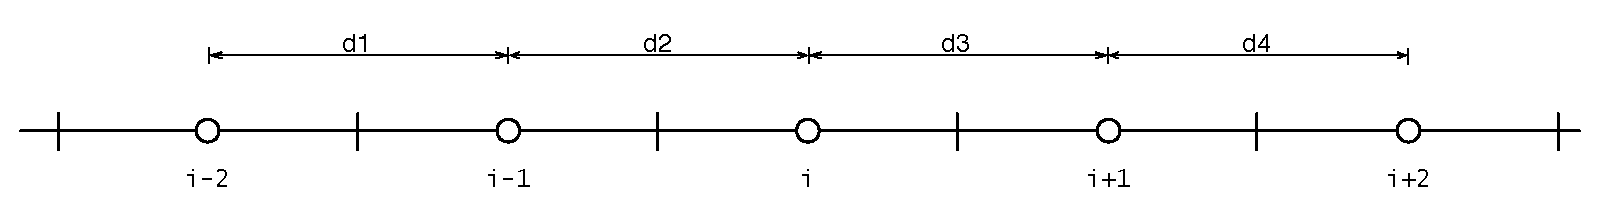
\includegraphics[width=15cm,clip]{muscl_stencil.eps}
\end{center}
\caption{MUSCLスキームのステンシル.d1,d2,d3,d4はセルセンタで定義される物理量の区間で,セル界面位置の速度の符号をs1,s2,s3,s4とする.}
\label{fig:muscl_stencil}
\end{figure}

コード中の実装は次の通り.
\[
\begin{array}{llll}
\vspace{1mm}
\mathrm{g6}; & \overline{\Delta^+_{i+1}} & = \mathrm{minmod}(\Delta^+_{i+1},\,b\Delta^-_{i+1}) & = \mathrm{s4} \cdot \mathrm{max}[0,\,\mathrm{min}\{ |\mathrm{d4}|,\, \mathrm{s4\,b\,d3}\} ] \\
\vspace{1mm}
\mathrm{g5}; & \overline{\Delta^-_{i+1}} & = \mathrm{minmod}(\Delta^-_{i+1},\,b\Delta^+_{i+1}) & = \mathrm{s3} \cdot \mathrm{max}[0,\,\mathrm{min}\{ |\mathrm{d3}|,\, \mathrm{s3\,b\,d4}\} ] \\
\vspace{1mm}
\mathrm{g4}; & \overline{\Delta^+_{i}} & = \mathrm{minmod}(\Delta^+_{i},\,b\Delta^-_{i}) & = \mathrm{s3} \cdot \mathrm{max}[0,\,\mathrm{min}\{ |\mathrm{d3}|,\, \mathrm{s3\,b\,d2}\} ] \\
\vspace{1mm}
\mathrm{g3}; & \overline{\Delta^-_{i}} & = \mathrm{minmod}(\Delta^-_{i},\,b\Delta^+_{i}) & = \mathrm{s2} \cdot \mathrm{max}[0,\,\mathrm{min}\{ |\mathrm{d2}|,\, \mathrm{s2\,b\,d3}\} ] \\
\vspace{1mm}
\mathrm{g2}; & \overline{\Delta^+_{i-1}} & = \mathrm{minmod}(\Delta^+_{i-1},\,b\Delta^-_{i-1}) & = \mathrm{s2} \cdot \mathrm{max}[0,\,\mathrm{min}\{ |\mathrm{d2}|,\, \mathrm{s2\,b\,d1}\} ] \\
\vspace{1mm}
\mathrm{g1}; & \overline{\Delta^-_{i-1}} & = \mathrm{minmod}(\Delta^-_{i-1},\,b\Delta^+_{i-1}) & = \mathrm{s1} \cdot \mathrm{max}[0,\,\mathrm{min}\{ |\mathrm{d1}|,\, \mathrm{s1\,b\,d2}\} ] \\
\end{array}
\]

%
\subsubsection{バイナリボクセルの場合の固体壁面境界処理}
バイナリボクセルによる物体形状表現では,計算空間内の任意のセルが物体(非流体)セルになる.対流項スキームの近似精度が高くなるとステンシルが広がり,参照セルが非流体セルのときの処理を適切に行わなくてはならない.

物理流束は\textbf{式(\ref{eq:physical flux ALE})}で表せるので,セルの6面について和をとると,対流項は次のように離散化される.

\begin{equation}
\frac{\partial f}{\partial x_j} \, \equiv \, \frac{1}{h} \sum  \limits_l \tilde{f}_l \,n_l 
\,=\, \frac{1}{h} \sum  \limits_l 
\frac{1}{2} { \left[ \, \left( f_R + f_L \right) \,-\, \left| (u-u^{\,g}) \right| \left( \varphi_R - \varphi_L \right) \, \right] }_{\,l} \, n_l
\label{eq:upwind approx}
\end{equation}

\noindent ここで$n_l$はセルの各面における外側法線であり,移流速度は各面に垂直な方向成分と考える.

バイナリボクセルでは,セルの状態を表すマスク関数$\phi$により形状を階段状に近似する.$\phi$は\textbf{式(\ref{eq:mask function})}として定義され,このマスク関数を用いて界面位置を調べ\footnote{事前に各セルの状態について,ビットフラグ(STATE\_BIT)にエンコードしておく.計算時には,デコードしたフラグから\textbf{式(\ref{eq:mask at cell face})}と式(\ref{eq:wall vel at cell face})を評価する.対流項部分の計算は演算量が多く,if文の分岐でも速度低下は小さいことを確認している(Intel Compiler 11.1).},壁面境界条件をスキーム中に取り込む\cite{akasaka:06:JSCES}.
\textbf{図\ref{fig:Mask pattern CC}}のようなコロケート配置におけるセルの状態パターンに対して,セルiでの計算を考える.

\begin{figure}[htbp]
\begin{center}
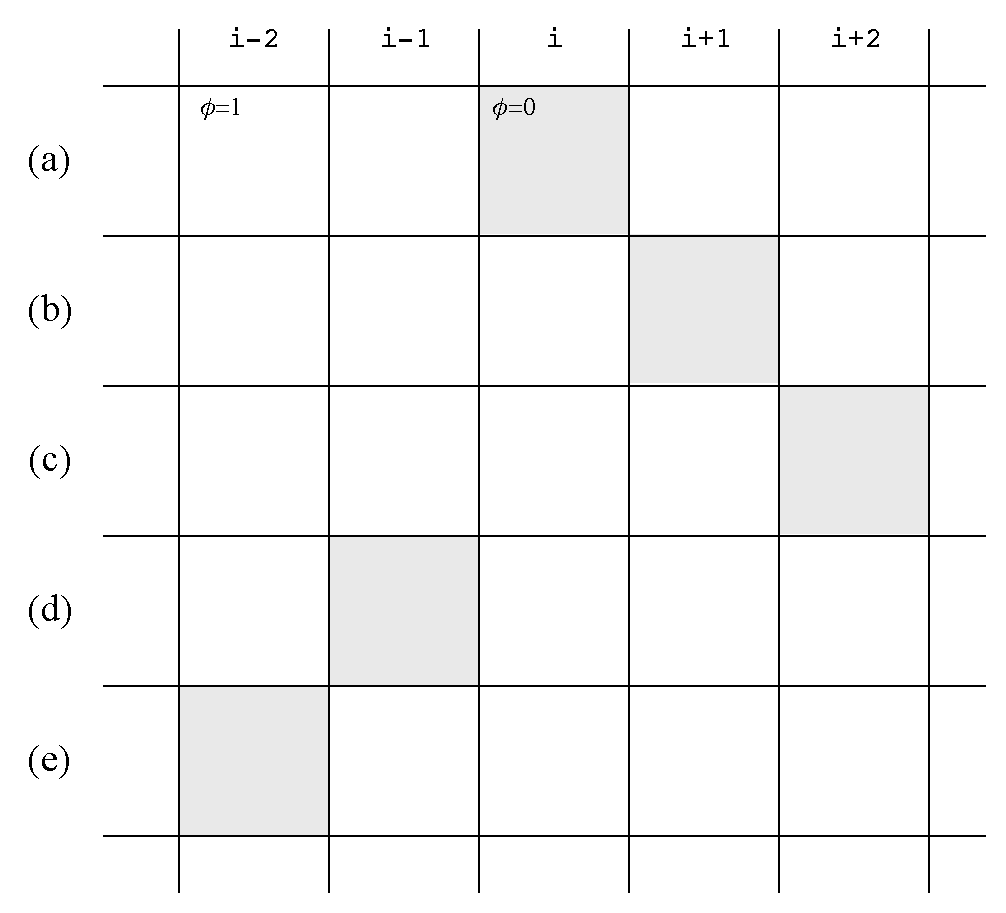
\includegraphics[width=8cm,clip]{mask_patternCC.eps}
\end{center}
\caption{対流項の計算で考慮するマスクパターン.網掛けの部分は非流体セル$\phi=0$,それ以外は流体セル$\phi=1$を示す.(a)$\sim$(e)のパターンは横方向に一次元的な分布を表している.}
\label{fig:Mask pattern CC}
\end{figure}

\begin{enumerate}
\item (a)の場合は,セルiの計算結果自体がマスクにより無効となるので考慮する必要はない.
\item ステンシルが$i\pm2$である(b)$\sim$(e)の場合は,参照値を修正する.
\item (b), (d)のパターン,つまり参照する$i\pm1$セルが固体の場合にも参照値を修正する.更に,$i\pm1/2$位置の流束は,固定壁面があるので$\tilde{f}=0$となる.次式のように界面のフラグによりマスクし,流束をゼロにするように実装している.
\begin{equation}
\phi_{\,i\pm1/2} \,=\, \phi_{i} \times \phi_{i\pm1} \,=\, \left\{
\begin{array}{ll}
0 & \mathrm{Wall\, boundary\, face}\\
1 & \mathrm{Fluid\, face}\\
\end{array} \right.
\label{eq:mask at cell face}
\end{equation}

\begin{equation}
\tilde{f}_{i\pm1/2} \,=\, \phi_{\,i\pm1/2} \, \tilde{f}_{i\pm1/2}
\label{eq:wall vel at cell face}
\end{equation}
\noindent ここで右辺の$\tilde{f}_{i\pm1/2}$は\textbf{式(\ref{eq:general flux form})}の評価式である.
\end{enumerate}

%
\subsubsection{参照値の修正}
\textbf{図\ref{fig:Mask pattern CC}}の各パターンに対して,対象セルの対流項を計算する場合の参照値の修正について考える.バイナリボクセルの形状表現では,物体境界は必ずセル界面にある.どのセル界面が固体境界面であるかは,セルの状態$\phi$を見て判断し,固体境界面における参照値は流体セル側からの線形分布を仮定する.パターン(b), (d)の場合,参照値$\varphi_{\,i\pm1}$を次のように近似する.$\varphi_{\,i\pm1/2\, face}$は境界値として与えられるものとする.

\begin{equation}
\varphi_{\,i\pm1} \,=\, 2 \,\varphi_{\,i\pm1/2\, face} - \varphi_{\,i}
\label{eq:solid face reference 1}
\end{equation}

\noindent 同様に,$\varphi_{\,i\pm2}$が参照値となる(c), (e)の場合についても$\varphi_{\,i\pm3/2\, face}$を境界値として与え,次式で修正する.

\begin{equation}
\varphi_{\,i\pm2} \,=\, 2 \,\varphi_{\,i\pm3/2\, face} - \varphi_{\,i\pm1}
\label{eq:solid face reference 2}
\end{equation}

%
\subsection{粘性項の扱い}
粘性項は,非圧縮条件を用いて簡略化して扱う.

\begin{equation}
\frac{1}{Re} \frac{\partial}{\partial x_j} \left( \frac{\partial u_i}{\partial x_j} + \frac{\partial u_j}{\partial x_i} \right)
\,=\, \frac{1}{Re} \frac{\partial}{\partial x_j} \left( \frac{\partial u_i}{\partial x_j} \right) 
\label{eq:viscous incomp approx}
\end{equation}

\noindent 対流項と同様に参照値の修正を行い,評価する.ベクトル成分$\varphi$について,Euler陽解法の場合について\textbf{式(\ref{eq:viscous approx})}に示す.

\begin{equation}
\frac{1}{Re} \frac{\partial}{\partial x_j} \left( \frac{\partial \varphi}{\partial x_j} \right)
\,\approx\, \frac{1}{Re\,h^2} \left\{\, \sum \limits_l \left( \varphi_{\,l} \right) \,-\, 6 \,\varphi_{\,i,j,k} \right\}
\label{eq:viscous approx}
\end{equation}

\noindent $\sum \limits_l \left( \varphi_{\,l} \right)$は,対象セルの隣接6セルの$\varphi$の和を意味する.


%
\subsection{境界条件処理}
\textbf{\ref{sec:fractional step}}のFractional Step法の手順では,疑似速度ベクトルを求めるプロセスで対流項と粘性項の計算を行い,その後境界条件処理を行う.
境界条件には,外部境界条件と計算領域内部で用いる境界条件の2種類が設定できる.
CBCソルバークラスで指定できる速度の境界条件を\textbf{表\ref{tbl:BCs of velocity}}に示す.

\begin{table}[htdp]
\small
\caption{計算領域内部と外部境界に指定できる速度境界条件の種類}
\begin{center}
\begin{tabular}{l|cc|ll} \toprule
境界条件の種類 & 内部 & 外部 & 外部境界の実装方式 & コメント\\ \midrule
壁面境界 & ○ & ○ & 流束形式 & フラグによりスキーム中に組み込まれている\\
対称境界 & - & ○ & 境界値指定 &\\
流入境界 & ○ & ○ & 流束形式 & Dirichlet型による速度指定(一定値と単振動条件)\\
流出境界 & ○ & ○ & 流束形式 & 対流流出,内部境界は面直のみ\\
遠方境界 & - & ○ & 境界値指定 & トラクションフリー\\
流入出境界 & - & ○ &  & 流出境界と,(流入として)遠方境界の切り替え\\
周期境界 & - & ○ & 境界値指定 & データコピー\\ \bottomrule
\end{tabular}
\end{center}
\label{tbl:BCs of velocity}
\end{table}

%
\subsubsection{速度境界条件のビットフラグ}
速度境界条件を認識するために,圧力の場合と同様にビットフラグを導入する.\textbf{図\ref{fig:bit flag V}}に示すように,各セルの6面についてフラグがセットされる.このフラグは各面に割り当てられた境界条件の識別子を示す.具体的には,媒質と境界条件の属性リストであるコンポーネントの登録番号である.CBCの実装では,コンポーネントは媒質と境界条件の個数を合わせて30個まで保持できる.各面に5ビット幅を割り当て,値の0は不使用(つまり,境界条件なし),31は外部境界の認識に利用している($2^5-2$個).\footnote{コンポーネント個数はParseBC::setControlVars()でチェック.}.\textbf{表\ref{tbl:Flags in bcv}}に具体的なビット割り当てを示す.

\begin{figure}[htbp]
\begin{center}
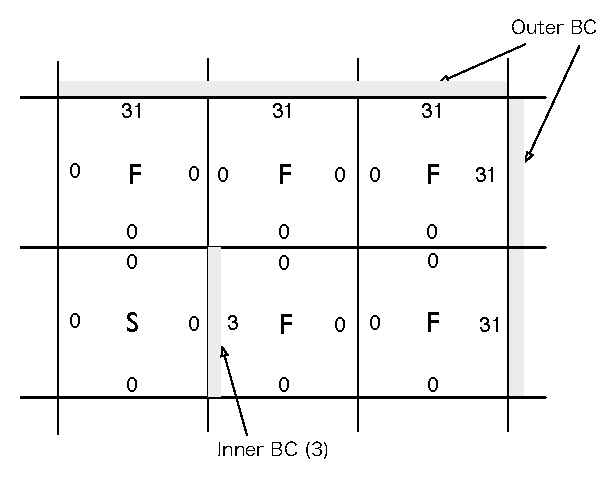
\includegraphics[width=8cm,clip]{bit_flag_V.eps}
\end{center}
\caption{速度境界条件に用いるビットフラグ.各セルについて,6つのフラグ(三次元の場合)を設定する.Sセルは固体セル,Fセルは通常の流体セルである.この例では内部境界条件として,コンポーネントの登録番号3の境界条件がひとつ指定されている.外部境界には,認識番号31が登録される.}
\label{fig:bit flag V}
\end{figure}

%
\subsubsection{内部境界条件}
固体壁条件については,計算空間内に任意の箇所に現れる可能性があるため,前述したようにフラグを用いて壁面の影響を流束形式によりスキームに導入する.
一方,流入と流出条件は,その処理は煩雑で効率的な実装が難しい場合が多いので,演算速度はあまり期待できない.しかしながら,指定する速度境界条件は一般的に局所的になる傾向があるため,境界条件処理かどうかを探索する範囲をバウンディングボックスで絞り込んでおくことにより,演算処理自体を少なくできる.
このため,コンポーネント単位で処理を行う.
境界条件の導入は,圧力の場合の\textbf{式(\ref{eq:ebcs_flagging})}と同様に,境界マスクと流束を次式により評価する.

\begin{equation}
\phi^{\,BC} \,=\, \left\{
\begin{array}{ll}
0 & \mathrm{Face\, that\, boundary\, condition\, is\, given}\\
1 & \mathrm{Normal\, face}\\
\end{array} \right.
\label{eq:mask function velocity}
\end{equation}

\begin{equation}
\tilde{f}_{i\pm1/2} \,=\, \phi^{\,BC} \tilde{f}_{i\pm1/2} \,+\, \left( 1-\phi^{\,BC} \right)\, \tilde{f}_{i\pm1/2}^{\,BC}
\label{eq:ebcs_flagging_vel}
\end{equation}

\noindent 実装としては,\textbf{式(\ref{eq:ebcs_flagging_vel})}を2パスで構成する.つまり,最初のループで固体壁の影響を考慮した流束$\tilde{f}_{i\pm1/2}$を計算し,境界条件が指定された面の流束は計算しない.次のループで,境界条件面のみ流束$\tilde{f}^{\,BC}_{i\pm1/2}$を計算し,寄与分を加算する.
内部境界条件は,ひとかたまりで格子線に沿って面直な流入・流出面をもつものを想定している.これらの境界条件は,流束形式でスキーム中に取り込まれる.また,補助的にセルフェイス位置の速度にも境界条件を与える.

%
\subsubsection{外部境界条件}
外部境界条件の実装には,2種類の方法を用いている.一つは,内部境界と同じく空間項の評価時に境界部分の流束を評価する方法である.もう一つは,一般的に行われている値を代入する方法である.後者の方法は,代入すべき位置(セル)が存在し,一意に決まる値で参照のみが行われる場合に用いる.

壁面境界は,空間項の評価時に壁面位置を感知し,その影響を境界条件として取り込む離散化を行っているので,特別な処理を必要としない.ただし,前処理として,指定された境界面に対して固体のIDをガイドセル部分に付与しておく.

流入と流出境界は,内部境界と同様な実装をで,処理単位は各面毎としている.

対称条件,遠方条件,周期条件については,境界値を指定する.


\pagebreak
%%%
\section{距離情報を用いた形状近似の解法}
形状の近似として,物理量の定義点から物体までの\hypertarget{tgt:dist_info_scheme}{距離情報のみを用いた形状近似}を考える.
前処理時の入力情報としてSTLなどの形状データを考え,含まれる三角形要素と格子の交点情報を計算する.
これより,距離情報が得られる.
この場合,入力のSTLが完全に形状を表現できていなくても,STLとして三角形要素が定義できていれば交点情報が必ず得られる.
また,定義点間に複数の交点があってもよい.
したがって,データフォーマットとして有効であれば,形状を完全に再現できていなくても,薄い物体でも扱うことが可能な利点がある.

%%
\subsection{実装の基本的な考え方}
コロケート格子における有限体積法ベースの流束計算に基づいて計算する.
物体近傍付近では,流束を構築する際に必要な速度の参照点の値を流体側から外挿することにより,物体の影響を考慮した流束を計算する.
したがって,物体の影響は全てセル界面の数値流束の近似に集約され,レギュラーのステンシルでの計算となる.

\textbf{図\ref{fig:distance stencil}}を参照して,セル$i$を積分する場合の壁面の影響をみる.
セル界面$i+1/2$側を考えると,次の2つの場合に分けられる.

\[
\begin{array}{lll}
\vspace{1mm}
(a) & 1/2 < d_i^+ < 1  & \varphi_{\,i+1/2}が定義でき,\tilde{f}_{\,i+1/2}が値をもつ. \\
\vspace{1mm}
(b) &  0 \le d_i^+ \le 1/2 & セル界面位置が固体内であるので\varphi_{\,i+1/2}が定義できない.\\  
\end{array}
\]

\begin{figure}[htbp]
\begin{center}
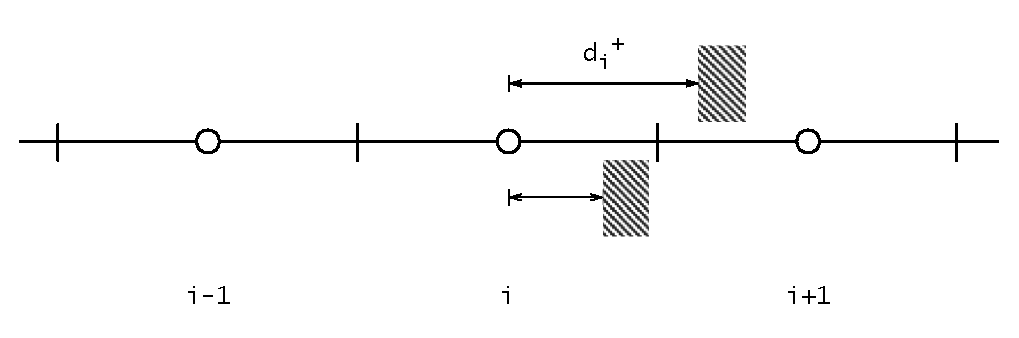
\includegraphics[width=10cm,clip]{distance_stencil.eps}
\end{center}
\caption{セル$i$を積分する場合の壁位置による影響.$d$は格子幅で正規化された無次元距離を表す.}
\label{fig:distance stencil}
\end{figure}

\noindent $d_i^{\pm}$は格子幅で正規化された距離で,$i$点における正負方向の距離を表し,[0,1]の値をとる.
$\varphi$は物理量で,例えば速度である.

(b)の場合には,セル界面位置が固体壁内部に位置するので,取り扱いを検討する.方法として,$\tilde{f}_{\,i+1/2}=0$と考えるやり方と,以下のように参照点の値を修正してそのまま計算するやり方が考えられる.とりあえず,後者を選択.
したがって,(a)の場合のみについて流束計算を考える.

参照点の外挿は,\textbf{図\ref{fig:stable extrapolation}}のように$d_i^+\rightarrow0$となっても破綻しないように次式を用いる~\cite{akasaka:10:JSME}.

\begin{equation}
\varphi_{\,i+1} \,=\, \frac{1}{1/2+d_i^+} \left[ \frac{3}{2}\varphi_{\,I} - (1-d_i^+)\,\varphi_{\,i-1/2} \right]
\label{eq:stable extrapolation}
\end{equation}

\noindent 同様に,界面$i-1/2$の場合には,
\begin{equation}
\varphi_{\,i-1} \,=\, \frac{1}{1/2+d_i^-} \left[ \frac{3}{2}\varphi_{\,I} - (1-d_i^-)\,\varphi_{\,i+1/2} \right]
\label{eq:stable extrapolation-}
\end{equation}

\noindent ここで$\varphi_I$は壁面の値で指定値である.また,$\varphi_{\,i\pm1/2}$の値は,定義されていなければ内挿する.

\begin{figure}[htbp]
\begin{center}
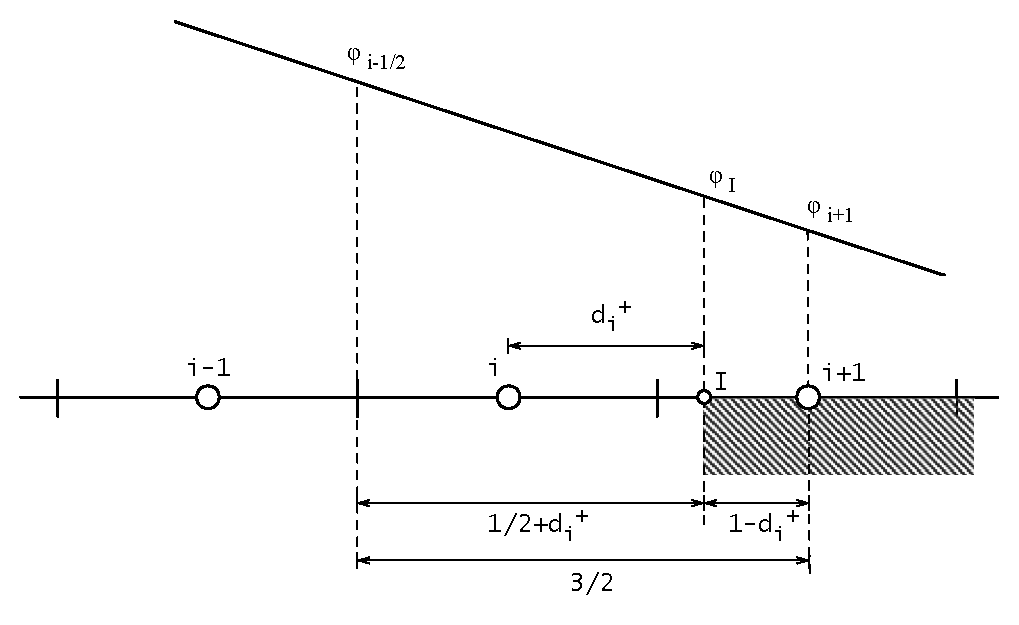
\includegraphics[width=11cm,clip]{extrapolation_stable.eps}
\end{center}
\caption{$(i+1)$セルが固体内にある場合の参照値$\varphi_{\,i+1}$の外挿.距離は格子幅$\Delta x$により正規化している.}
\label{fig:stable extrapolation}
\end{figure}

あるいは,少々不安定な実装として,次も考慮.
\begin{equation}
\displaystyle{ \varphi_{\,i\pm1} \,=\, \frac{1}{d_i^{\pm}} \left[ \varphi_{\,I} - \left( 1 - d_i^{\pm} \right) \varphi_{\,i} \right] }
\label{eq:unstable}
\end{equation}


%%
\subsection{距離情報を用いたMUSCLスキームの実装}
セル$i$に関する流束計算を高次精度のスキームを用いるとステンシルが広がる.
参照点間にカットが入るパターンに分類して,スキームの実装を述べる.

%
\subsubsection{対流項スキーム実装の詳細}
%まず,正負の各方向で$0 \le d_i^{\pm} \le 1/2 \, \mapsto \,\tilde{f}_{i\pm1/2}=0$とする.
%実装としては,次式のようにマスク関数$\chi$をかけて流束をゼロに強制する.

%\begin{equation}
%\tilde{f}_{\,i\pm1/2} \,=\,
%\frac{1}{2} { \left[ \, \left( f_R + f_L \right) \,-\, \left| (u-u^{\,g}) \right| \left( \varphi_R - \varphi_L \right) \, \right] }_{\,i\pm1/2} \, \chi
%\label{eq:masked flux form}
%\end{equation}

%\[
%\hspace{1cm}
%\chi \,=\,
%\left\{
%\begin{array}{ll}
%\vspace{1mm}
%0 & (0 \le d_i^{\pm} \le 1/2)\\
%\vspace{1mm}
%1 & (d_i^{\pm} > 1/2)\\
%\end{array}
%\right.
%\]

MUSCLスキームは片側3点の参照点をもつので,\hypertarget{tgt:modify by cut}{参照する物理量が壁面位置による修正}が必要かどうかを見ていく.

%
\paragraph{$\tilde{f}_{i-1/2}$の評価}
$\tilde{f}_{i-1/2}$を評価する場合,$u_{\,i-1/2}$の符号により参照するセルが異なる.
\[
\tilde{f}_{i-1/2}\,=\,
\left\{
\begin{array}{ll}
\vspace{1mm}
f(\varphi_{\,i-2},\,\varphi_{\,i-1},\,\varphi_{\,i}) & u_{\,i-1/2}\ge0\\
\vspace{1mm}
f(\varphi_{\,i-1},\,\varphi_{\,i},\,\varphi_{\,i+1}) & u_{\,i-1/2}<0\\
\end{array}
\right.
\]

壁面の影響による修正が必要な場合とは,参照する定義点間に交点が存在する場合である.
各セルで計算した距離情報の値を判定すれば,交点があるかどうかわかる.
つまり,$d\ne1$であれば交点が存在し,参照するセルの値を修正する必要がある.

%
\vspace{5mm}
\subparagraph{$u_{\,i-1/2}\ge0$の場合}
参照するセルは$(i-2,\,i-1,\,i)$であるが,$i$セルについての計算なので,修正対象となるセルは$(i-2,\,i-1)$セルである.

\begin{enumerate}
\item \textbf{図\ref{fig:stencil case 1}}に示すように,もし$d_i^- \ne 1$であれば,$(i-1)\sim (i)$間に交点が存在し,\textbf{式(\ref{eq:stable extrapolation-})}により$\varphi_{\,i-1}$の参照値を修正する.
\vspace{1mm}
\item 同じように,$d_{i-1}^- \ne 1$であれば,$\varphi_{\,i-2}$の修正が必要になる.
\begin{equation}
\varphi_{\,i-2} \,=\, \frac{1}{1/2+d_{i-1}^-} \left[ \frac{3}{2}\varphi_{\,I} - (1-d_{i-1}^-)\,\varphi_{\,i-1/2} \right]
\label{eq:modify i-2}
\end{equation}
\end{enumerate}

\begin{figure}[htbp]
\begin{center}
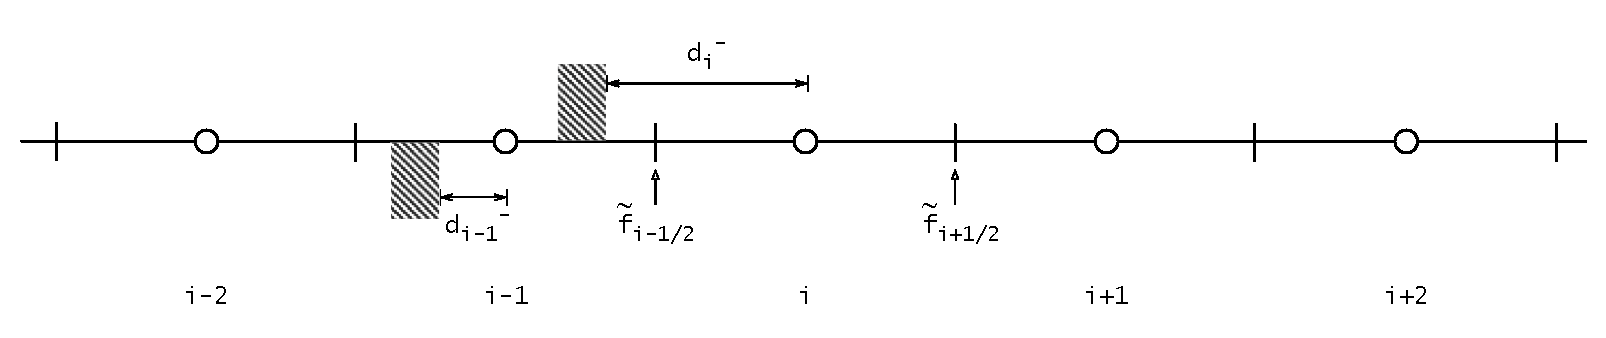
\includegraphics[width=15cm,clip]{stencil_case1.eps}
\end{center}
\caption{$\tilde{f}_{i-1/2}$評価時の$u_{\,i-1/2}\ge0$の場合の修正の判定.このときステンシルは$(i-2,\,i-1,\,i)$で,壁面の影響による修正を考慮する対象は$(i-2,\,i-1)$.}
\label{fig:stencil case 1}
\end{figure}


%
\vspace{5mm}
\subparagraph{$u_{\,i-1/2}<0$の場合}
参照するセルは$(i-1,\,i,\,i+1)$であるが,$i$セルについての計算なので,壁面が存在する場合の修正対象は$(i-1,\,i+1)$セルである.

\begin{enumerate}
\item \textbf{図\ref{fig:stencil case 2}}に示すように,もし$d_i^- \ne 1$であれば,$(i-1)\sim (i)$間に交点が存在し,\textbf{式(\ref{eq:stable extrapolation-})}により$\varphi_{\,i-1}$の参照値を修正する.
\vspace{1mm}
\item $d_{i}^+ \ne 1$であれば,\textbf{式(\ref{eq:stable extrapolation})}により$\varphi_{\,i+1}$を修正する.
\end{enumerate}

\begin{figure}[htbp]
\begin{center}
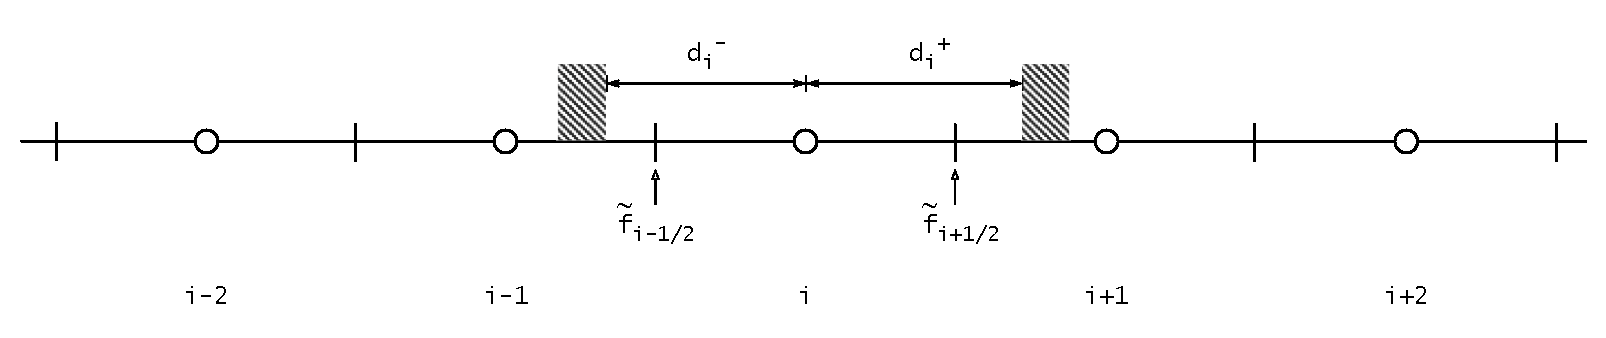
\includegraphics[width=15cm,clip]{stencil_case2.eps}
\end{center}
\caption{$\tilde{f}_{i-1/2}$評価時の$u_{\,i-1/2}<0$の場合,ステンシルは$(i-1,\,i,\,i+1)$で修正対象は$(i-1,\,i+1)$.$\tilde{f}_{i+1/2}$評価時の$u_{\,i+1/2}\ge0$の場合のステンシルも同様.}
\label{fig:stencil case 2}
\end{figure}


%
\paragraph{$\tilde{f}_{i+1/2}$の評価}
$\tilde{f}_{i+1/2}$を評価する場合,$u_{\,i+1/2}$の符号により参照するセルが異なる.
\[
\tilde{f}_{i+1/2}\,=\,
\left\{
\begin{array}{ll}
\vspace{1mm}
f(\varphi_{\,i-1},\,\varphi_{\,i},\,\varphi_{\,i+1}) & u_{\,i+1/2}\ge0\\
\vspace{1mm}
f(\varphi_{\,i},\,\varphi_{\,i+1},\,\varphi_{\,i+2}) & u_{\,i+1/2}<0\\
\end{array}
\right.
\]


%
\vspace{5mm}
\subparagraph{$u_{\,i+1/2}\ge0$の場合}
修正対象となるセルは$(i-1,\,i+1)$セルである.

\begin{enumerate}
\item \textbf{図\ref{fig:stencil case 2}}に示すように,もし$d_i^- \ne 1$であれば,$(i-1)\sim (i)$間に交点が存在し,\textbf{式(\ref{eq:stable extrapolation-})}により$\varphi_{\,i-1}$の参照値を修正する.
\vspace{1mm}
\item $d_{i}^+ \ne 1$であれば,\textbf{式(\ref{eq:stable extrapolation})}により$\varphi_{\,i+1}$を修正する.
\end{enumerate}


%
\vspace{5mm}
\subparagraph{$u_{\,i+1/2}<0$の場合}
修正対象となるセルは$(i+1,\,i+2)$セルである.

\begin{enumerate}
\item \textbf{図\ref{fig:stencil case 3}}に示すように,もし$d_i^+ \ne 1$であれば,\textbf{式(\ref{eq:stable extrapolation})}により$\varphi_{\,i+1}$の参照値を修正する.
\vspace{1mm}
\item $d_{i+1}^+ \ne 1$であれば,次式により$\varphi_{\,i+2}$を修正する.
\begin{equation}
\varphi_{\,i+2} \,=\, \frac{1}{1/2+d_{i+1}^+} \left[ \frac{3}{2}\varphi_{\,I} - (1-d_{i+1}^+)\,\varphi_{\,i+1/2} \right]
\label{eq:modify i+2}
\end{equation}
\end{enumerate}

\begin{figure}[htbp]
\begin{center}
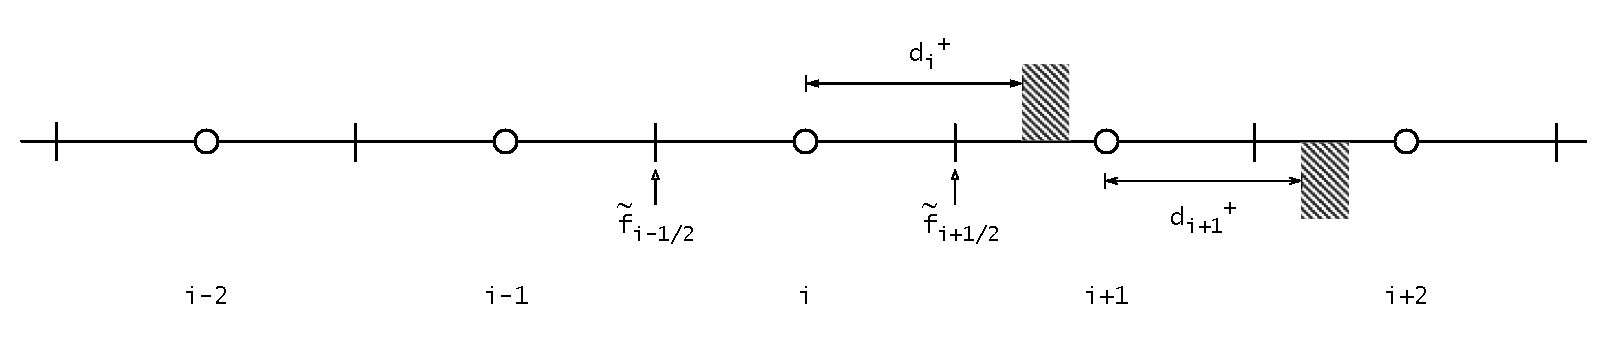
\includegraphics[width=15cm,clip]{stencil_case3.eps}
\end{center}
\caption{$\tilde{f}_{i+1/2}$評価時の$u_{\,i+1/2}<0$の場合の修正の判定.}
\label{fig:stencil case 3}
\end{figure}

%
\subsubsection{粘性項の計算}
粘性項を二次精度の中心差分で近似する場合は,\textbf{図\ref{fig:stencil case 1}}などでセル$(i-1,\,i+1)$について,壁面の影響を考慮して参照値の修正をすればよい.
あとは,参照値を用いて通常どおりのスキームにより計算をする\footnote{実装としては,壁面の影響を修正する処理を二重にするのを避けるため,対流項スキームとは分けず同一関数内で処理する.}.

%
\subsubsection{速度ベクトル発散の計算}
Poisson方程式のソース項や収束判定に用いる速度ベクトルの発散の計算について説明する.
\textbf{図\ref{fig:div operator}}に示すセルaは通常のステンシルで計算できる.一方,セルbとセルcは壁面の影響があるので,参照値を修正する.
修正の方法は前述した方法を適用する.

\begin{figure}[htbp]
\begin{center}
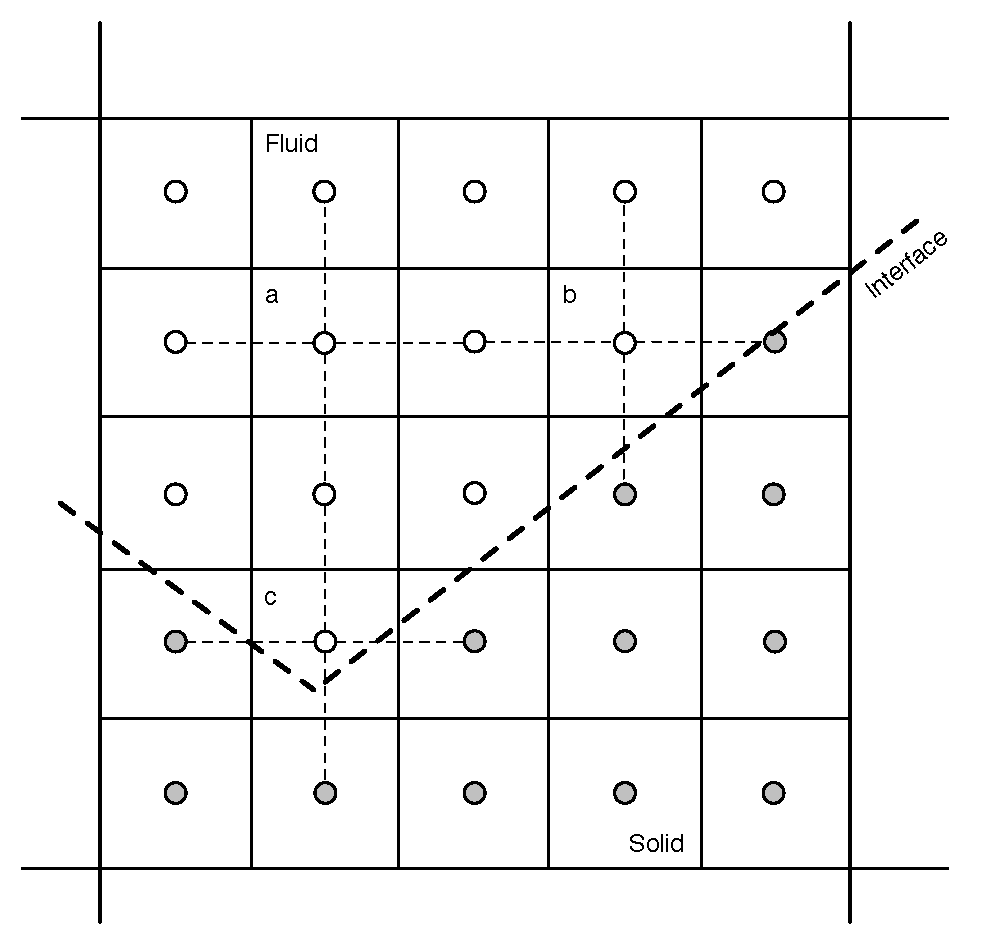
\includegraphics[width=10cm,clip]{div_operator.eps}
\end{center}
\caption{$\partial u_i / \partial x_i$の計算と圧力計算.○はセルセンター位置が流体で計算するセル,●は計算しないセル.aは通常のステンシル,セルb,cにはそれぞれ2方向,3方向の修正が必要.}
\label{fig:div operator}
\end{figure}

%
\subsection{圧力計算}
圧力計算の方法として,\hyperlink{tgt:Poisson Binary}{Binary近似}の方法と法線情報を用いて形状近似度を改善する方法が適用可能.

%
\subsubsection{バイナリ近似の前処理}
距離情報を用いた計算で圧力をバイナリで扱う場合,前処理時に距離情報を用いて\hyperlink{tgt:EBCS poisson BC}{ノイマン条件}をセットしておく.
各セル定義点で計算された6方向の距離情報をみて,それらが1.0\footnote{格子幅$\Delta x$で正規化.}でなければ壁面が存在することになる.

%
\subsubsection{法線を利用した参照点への内挿}
法線情報を用いて精度を改善する方法について述べる.


%
\subsection{物体との交点を含むセル間の速度ベクトルの内挿}
セルセンター速度からセルフェイス速度への内挿処理が必要になるが,物体との交点を含むセル間では注意する必要がある.
\textbf{図\ref{fig:interpolation cc2cf}}には,セル{i}の両側のセルフェイス位置の速度$\varphi_{\,i+1/2}, \varphi_{\,i-1/2}$に内挿する処理を示している.
左右のセルフェイスへは,それぞれ次式で内挿する.

\begin{equation}
\displaystyle{ \varphi_{\,i\pm1/2} \,=\, \frac{1}{d_i^{\pm}} \left[ \frac{1}{2} \varphi_{\,w} + \left( d_i^{\pm} - \frac{1}{2} \right) \varphi_{\,i} \right] }\\
\label{eq:interpolation cc2cf}
\end{equation}


\begin{figure}[htbp]
\begin{center}
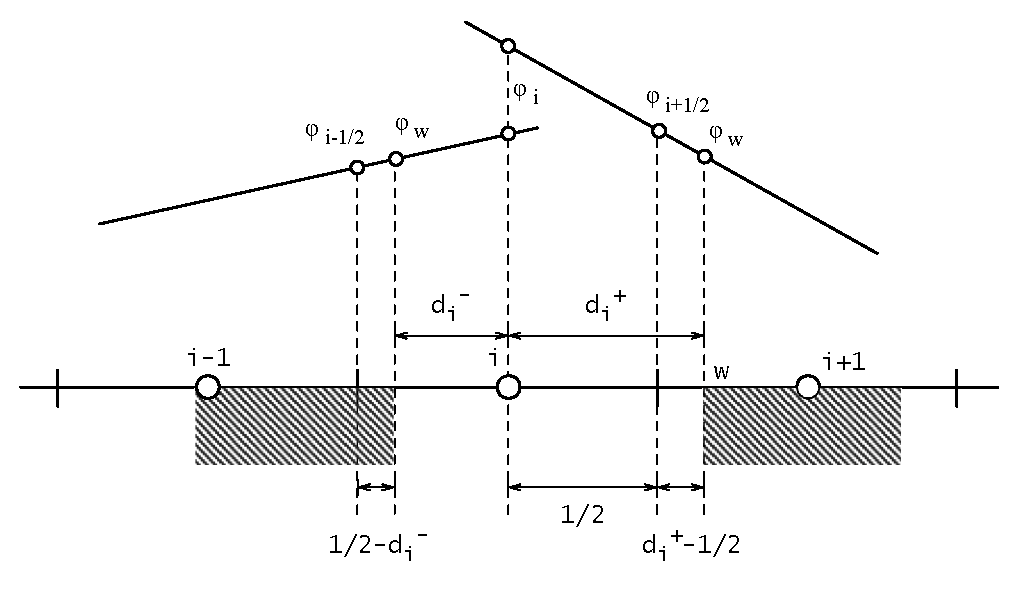
\includegraphics[width=11cm,clip]{intp_cut.eps}
\end{center}
\caption{セルセンターの速度ベクトルからセルフェイスの速度ベクトルへの内挿.}
\label{fig:interpolation cc2cf}
\end{figure}

セル間に薄い物体がある場合には,共有する同一のセル界面でも異なる参照値をもつことになる.
この場合には,セルフェイスの値を保持して,それを積分するやり方ではなく,セルセンターの値に直接積分して集約するようにする.
また,ここで述べる方法は\hyperlink{tgt:modify by cut}{前述した方法}とは異なるので,暫定的な実装.

\pagebreak

%%%
\section{体積力を用いた境界条件}
複雑形状周りの流れを解析する場合,Cartesian Methodは格子作成の労力を低減できる点で魅力的な方法である.
格子生成の手間は減少するが,それと引き換えにソルバー側で任意の形状の境界条件を取り扱う工夫が必要になる.
また,形状近似のレベルに応じて必要な形状パラメータを得る前処理プログラムの開発が必要となる.
Cartesian Methodでは格子密度が重要なパラメータとなるが,計算機資源や計算時間の制限から十分な格子が得られない場合がある.
現象の中に空間スケールの異なる流れがあり相互に影響するような問題,例えば,多孔質層を通過する大空間の流れを解析する場合,興味の対象は大空間内の流動挙動であり,多孔質層内はマクロに見て適切な流れ場になっていればよい.
この場合,多孔質部分はダルシー則などによりモデル化される.
メッシュ解像度以下の微細な構造が流動特性に与える影響は,ダルシー則などのように理論的,あるいは実験式などで与えられる場合も多い.
自動車のエンジンルーム内の流れを解析する場合にも,エンジンルーム内に配置される熱交換器は同様の特徴をもち,その特性は通過風速と圧力損失量の関係として実験式で与えられる.
本節ではCartesian Methodで有用な\hypertarget{tgt:body_force_bc}{体積力を用いた種々の境界条件}の導入について述べる.

%
\subsection{外力項による境界条件の導入}
\label{sec:external force method}

\textbf{式(\ref{eq:NS_ext_force ND})}に示すNavier-Stokes方程式中の外力項$F_{i}$を通して,体積力の形で様々な効果を導入する.各論の前に,まずFractional Step法に従って,大まかな手順を示す.

\begin{equation}
{\frac{\partial u_{i}}{\partial t}}^{n+1} + \frac{\partial}{\partial x_{j}} \left({ u_{i} u_{j} }\right)
\, =\,
- \frac{\partial p}{\partial x_{i}} + \frac{1}{Re} \frac{\partial}{\partial x_{j}} 
\left({ \frac{\partial u_{i}}{\partial x_{j}} + \frac{\partial u_{j}}{\partial x_{i}} }\right) + F_{i}
\label{eq:NS_ext_force ND}
\end{equation}


体積力として与える境界条件の位置は,ボクセルモデルのセル毎に付与されるIDにより指定される.
このIDにより,境界条件の種類と計算空間内の場所が特定できる.
この境界条件は,コンポーネントとして扱う\footnote{コンポーネントは,計算空間内に配置される境界条件や媒質を扱うための仕組みである.}.
体積境界条件コンポーネントの占有率$\beta$をセル中心で次のように定義する.

\begin{equation}
\left \{
\begin{array}{ll}
\beta \,=\, 0.0 & (Fluid)\\
0.0\le \beta \le 1.0 & (Component) \end{array}
\right. 
\label{eq:component fraction}
\end{equation}

$\beta$を用いると,\textbf{式(\ref{eq:NS_ext_force ND})}は次のように書ける.外力項を時間に関して陽的に扱う場合,非定常性が強い場合には不安定になることが懸念されるため,外力項を陰的に扱いPoissonの反復過程に組み込む.

\begin{equation}
{\frac{\partial u_{i}}{\partial t}}^{n+1} + \frac{\partial}{\partial x_{j}}{\left({ u_{i} u_{j} }\right)}^{n}
\, =\,
- {\frac{\partial p}{\partial x_{i}}}^{n+1} + \frac{(1-\beta)}{Re} \frac{\partial}{\partial x_{j}} \left({ {\frac{\partial u_{i}}{\partial x_{j}}}^{n} + {\frac{\partial u_{j}}{\partial x_{i}}}^{n} }\right) + \beta {F_{i}}^{n+1}
\label{eq:NS_ext_force ND2}
\end{equation}

Euler 陽解法を用いると疑似ベクトルは,

\begin{equation}
{u_{i}}^{*}
\, =\, 
{u}_{i}^{n}\, -\,\mathrm{\Delta}{t} \left\{{ \frac{\mathrm{\partial}}{\mathrm{\partial}{x}_{j}}{\left({{u}_{i}{u}_{j}}\right)}^{\hspace{0.3em}{n}}\mathrm{{-}}\,\frac{(1-\beta)}{Re} \frac{\partial}{\partial x_{j}} \left({ {\frac{\partial u_{i}}{\partial x_{j}}}^{n} + {\frac{\partial u_{j}}{\partial x_{i}}}^{n} }\right) }\right\}
\label{eq:pseudo_vector forcing}
\end{equation}

射影ステップは,
\begin{equation}
{u_{i}}^{n+1} \,=\, {{u}_{i}}^{*} - \Delta{t} \left({ {\frac{\partial p}{\partial x_{i}}}^{n+1} - \beta {F_{i}}^{n+1} }\right)
\label{eq:projection forcing}
\end{equation}

圧力反復は連続の式から導かれ,次のようになる.

\begin{equation}
\frac{\partial}{\partial x_i} {\left( \frac{\partial p}{\partial x_i} \right)}^{n+1}
\,=\,
\frac{1}{\Delta t} \frac{ {\partial u_i}^*}{\partial x_i}
\,+\,
\frac{\partial}{\partial x} \left( \beta {F_i}^{n+1} \right)
\label{eq:iteration forcing}
\end{equation}

\vspace{3mm}


多孔質内における流動は,対流項の影響よりも粘性力の影響が大きく,ダルシー抵抗と圧力のバランスが重要になる.\textbf{式(\ref{eq:iteration forcing})}による外力の扱いはこの事実を直接的に反映しており,多孔質内流動などではより早い収束が期待できる.


%
\subsection{熱交換器(圧力損失部)}
熱交換器の特性を想定した圧力損失モデルを外力項の形式で表し,\textbf{\ref{sec:external force method}}に示した計算アルゴリズム中にコンシステントに組み込む.
熱交換器は\textbf{図\ref{Heat exchanger}}のようにチューブとフィンから構成され,熱交換器面に対して面直の法線方向に流れが限定される.熱交換器の流動特性として,平均通過風速と熱交換器部で発生する静圧損失のマクロな関係がJISで定められる測定により得られる.これは\textbf{図\ref{pressure drop}}に示すようにほぼ二次関数としてモデル化できる.
熱交換器モデルとしては,下記の特性をもつ数値モデルを考える.

\begin{figure}[htbp]
  \begin{minipage}{.47\textwidth}
  	\begin{center}
  	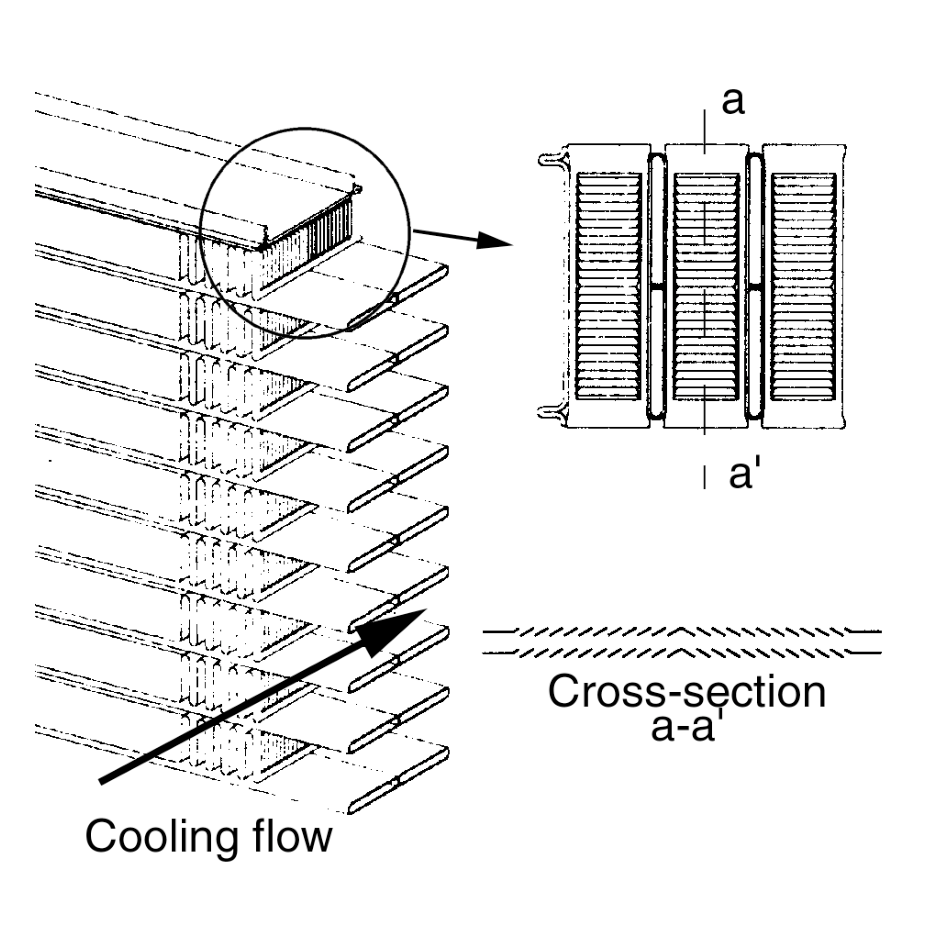
\includegraphics[width=8cm,clip]{HeatExchanger.eps}
  	\end{center}
  	\caption{自動車用熱交換器の構造}
	\label{Heat exchanger}
  \end{minipage} \hfill
  \begin{minipage}{.47\textwidth}
	\begin{center}
  	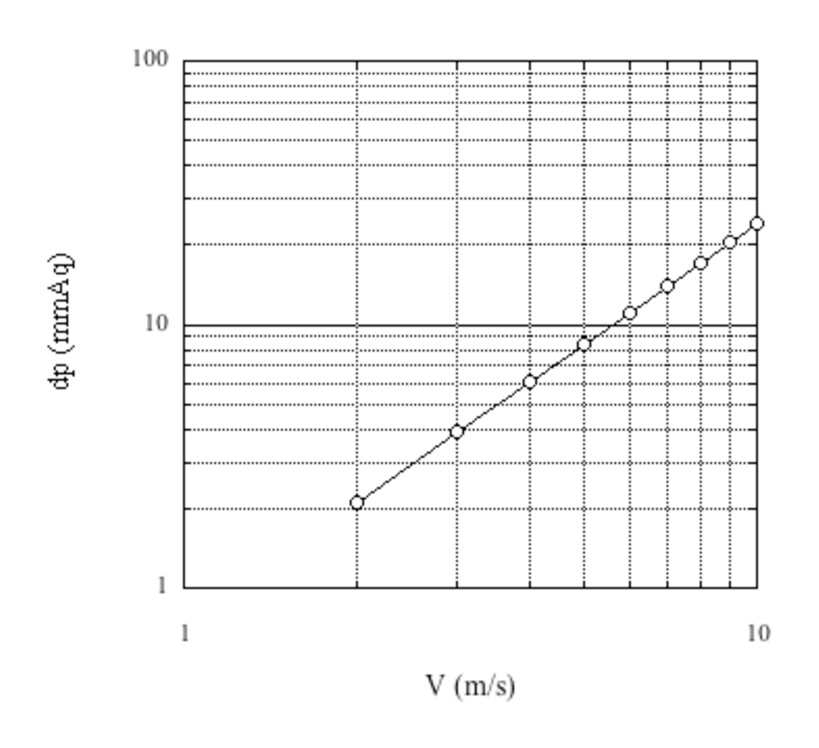
\includegraphics[width=7.5cm,clip]{Pressureloss.eps}
  	\end{center}
  	\caption{熱交換器の通過風量(風速)と圧力損失量の測定値}
  	\label{pressure drop}
  \end{minipage}
\end{figure}

\begin{itemize}
\item 流れの方向は法線${n_{i}}^{\prime}$方向(\textbf{図\ref{Heat exchanger}}中の矢印の方向)に限定される.
マクロな視点から${n_{i}}^{\prime}$と垂直方向には,チューブにより流れが発生しない.
\item ${n_{i}}^{\prime}$ 方向に$\Delta p^{\prime} = f({u_{i}}^{\prime})$の圧力損失が発生する.
\item 関数形として二次多項式の形式と離散データ形式を考慮する.
\item 熱交換器部では,傾斜して配置された場合の入口損失なども実験式に含まれることとする.
\end{itemize}

以下の基礎式を考える.

\begin{equation}
{\frac{\partial{{u}_{i}}^{\prime}}{\partial{{x}_{i}}^{\prime}}}^{n+1} \, =\, {0}
\label{eq:continuity_pl}
\end{equation}

\begin{equation}
{\frac{\partial{u_{i}}^{\prime}}{\partial{t}^{\prime}}}^{n+1} + \frac{\partial}{\partial{x_{j}}^{\prime}} \left({ {u_{i}}^{\prime} {u_{j}}^{\prime} }\right)
\, =\,
- \frac{\partial{p}^{\prime}}{\partial{x_{i}}^{\prime}} + \frac{\partial {\tau_{ij}}^{\prime}}{\partial{x_{j}}^{\prime}}
\label{eq:NS1_pl}
\end{equation}

\begin{equation}
{\tau_{ij}}^{\prime}
\,=\,
\nu \left({ \frac{\partial{u_{i}}^{\prime}}{\partial{x_{j}}^{\prime}} + \frac{\partial{u_{j}}^{\prime}}{\partial{x_{i}}^{\prime}} }\right)
\label{eq:tensor_pl}
\end{equation}

熱交換器部分では粘性項の影響を無視し,熱交換器による圧力損失の影響を${F_{R}}_{i}^{\prime}$とすると,

\begin{equation}
{\frac{\partial{u_{i}}^{\prime}}{\partial{t}^{\prime}}}^{n+1} + \frac{\partial}{\partial{x_{j}}^{\prime}} \left({ {u_{i}}^{\prime} {u_{j}}^{\prime} }\right)
\, =\,
- {\frac{\partial{p}^{\prime}}{\partial{x_{i}}^{\prime}}}^{R} + {F_{R}}_{i}^{\prime}
\label{eq:NS2_pl}
\end{equation}

ここで,圧力勾配項は熱交換器による静圧変化分を表す.
熱交換器の占有率として\textbf{式(\ref{eq:component fraction})}の$\beta$を用い,\textbf{式(\ref{eq:NS1_pl})}と\textbf{式(\ref{eq:NS2_pl})}をまとめると,

\begin{equation}
{\frac{\partial{u_{i}}^{\prime}}{\partial{t}^{\prime}}}^{n+1} + \frac{\partial}{\partial{x_{j}}^{\prime}} \left({ {u_{i}}^{\prime} {u_{j}}^{\prime} }\right)
\, =\,
- {\left\{{ \beta {\frac{\partial{p}^{\prime}}{\partial{x_{i}}^{\prime}}}^{R} + (1-\beta) \frac{\partial{p}^{\prime}}{\partial{x_{i}}^{\prime}} }\right\}}^{n+1} + (1-\beta) \frac{\partial{\tau_{ij}}^{\prime}}{\partial{x_{j}}^{\prime}}
\label{eq:NS3_pl}
\end{equation}

$\beta=0.0$のとき,つまり流体部分では,\textbf{式(\ref{eq:NS3_pl})}は\textbf{式(\ref{eq:NS1_pl})}と等価である.

ここで,熱交換器の圧力損失について考える.
コア厚さ$\Delta r^{\prime}$の熱交換器で${\Delta p^{\prime}}^{R}\, =\, f({{u_{i}}^{\prime}}^{R})$の圧力損失が得られる.
圧力損失は速度に比例して大きくなり,通常の圧力勾配と同じ符号となる.
つまり,正の向きの速度ベクトルに対して逆圧力勾配となる.

\begin{equation}
{F_{R}}_{i}^{\prime} \, =\,
-{sgn} \left({ {u_{i}}^{\prime} }\right) {\frac{\Delta{p}^{\prime}}{\Delta{r}^{\prime}}}^{R} {n_{i}}^{\prime}
\label{eq:Ploss_pl}
\end{equation}


\textbf{式(\ref{eq:Ploss_pl})}の無次元化にあたり,$sgn{({u_{i}}^{\prime})}, \, {n_{i}}^{\prime}$は単に方向を表すものであるので,無次元化には影響しない点に注意する.
熱交換器部の圧力勾配は,流れ場の圧力勾配に対して線形な関係を仮定すると,次のようにモデル化できる.

\begin{equation}
\frac{{\partial{p}^{\prime}}^{R}}{\partial{x_{i}}^{\prime}}
\, =\,
\frac{\partial{p}^{\prime}}{\partial{x_{i}}^{\prime}} + {F_{R}}_{i}^{\prime}
\label{eq:Ploss2_pl}
\end{equation}

\begin{equation}
{\frac{\partial{u_{i}}^{\prime}}{\partial{t}^{\prime}}}^{n+1} + \frac{\partial}{\partial{x_{j}}^{\prime}} \left({ {u_{i}}^{\prime} {u_{j}}^{\prime} }\right)
\, =\,
- {\frac{\partial{p}^{\prime}}{\partial{x_{i}}^{\prime}}}^{n+1} + (1-\beta) \frac{\partial{\tau_{ij}}^{\prime}}{\partial{x_{j}}^{\prime}} + \beta {{F_{R}}_{i}^{\prime}}^{n+1}
\label{eq:NS4_pl}
\end{equation}

\textbf{式(\ref{eq:NS4_pl})}を無次元化すると,\textbf{式(\ref{eq:NS_ext_force ND})}の形式になる.

%
\subsubsection{熱交換器の境界条件}
熱交換器に特有の境界条件として,\textbf{式(\ref{eq:projection_pl})}に従い,速度ベクトルを熱交換器の流出方向(面法線ベクトル${n_{i}}^{\prime}$)へ射影する.

\begin{equation}
{u_{i}}^{*}
\, =\,
(1-\beta) {u_{i}}^{*} \,+\, \beta \left|{ {u_{i}}^{*} }\right| n_{i}
\label{eq:projection_pl}
\end{equation}

もし,単に\textbf{式(\ref{eq:projection_ng_pl})}により方向を強制すると,ベクトルの成す角度が大きくなった場合,内積の値が小さくなり,速度ベクトルの大きさが小さくなる.そうすると,保存則を満たすように逆に圧力勾配が大きくなり熱交換器部分で加速するようになる.したがって,動圧が変化しないように\textbf{式(\ref{eq:projection_pl})}を採用する.

\begin{equation}
{u_{i}}^{*}
\, =\,
(1-\beta) {u_{i}}^{*} + \beta \left({ {u_{i}}^{*} n_{i} }\right) n_{i}
\label{eq:projection_ng_pl}
\end{equation}

\noindent $\beta$と$F_{i}$の各値は,速度ベクトル成分のセルセンタの点で定義されることに注意する.

熱交換器内部では,\textbf{式(\ref{eq:iteration forcing})}の右辺第3項もゼロになる.したがって,Laplace 方程式を解いていることになり,単に前後の圧力差から平滑化を行うことになる.これは,熱交換器の前後で圧力勾配の跳びが発生し,内部は流速一定の流れ場になっているとする仮定とコンシステントである.\textbf{式(\ref{eq:iteration forcing})}を解いて得られた圧力場は,熱交換器部で通過風速に応じた圧力勾配となっている.

本手法は流体の圧力場の一部分の勾配を指定しながら Poisson 方程式を解いている.これは,圧力 Poisson 方程式中において勾配の境界条件を満たすように解いていることと同じで,Liuら\cite{Liu:00:JCP}の Laplace/Poisson 方程式への境界条件の導入方法と基本的に同じアイデアである.また,圧力と速度の同時緩和を行いながら圧力損失項をアップデートするため,n+1 ステップでより良い近似になっている.


%
\subsubsection{圧力損失パラメータ}
圧力損失パラメータは,熱交換器の性能試験結果により得られる.$\Delta p-V$ の性能線図を$[mmAq - m/s]$ 単位とした場合のパラメータの取得について示す.\textbf{図\ref{pressure drop}}のように横軸に熱交換器の平均通過流速 $V^{\prime} [m/s]$, 縦軸に圧力損失ヘッド $h^{\prime} [mmAq]$ とする.多くの場合,流速の二次曲線で近似できる.プライム[$\,^{\prime}$] は有次元量を示すものとして,

\begin{equation}
{h}^{\prime} 
\,=\,
\left\{{ \begin{array}{ll}
c_{1} {u^{\prime}}^{2} \,+\, c_{2} u^{\prime} \,+\, c_{3} & \left({ u^{\prime} \geq {u_{th}}^{\prime} }\right)\\
c_{4} {u^{\prime}}^{2} & \left({ u^{\prime} < {u_{th}}^{\prime} }\right)
\end{array}}\right. \quad [mm]
\label{eq:coef1_pl}
\end{equation}

\noindent 係数$c_{4}$の式は速度が小さいときに圧力損失量をゼロに漸近させるためのもので,閾値${u_{th}}^{\prime}$で切り替える.\\

圧力損失と$\Delta r^{\prime} \,[mm]$の厚さの熱交換器部での圧力勾配は次のようになる.

\begin{equation}
{\Delta p}^{\prime} \,=\, {\rho_{w}}^{\prime} g h^{\prime} \times 10^{-3} \quad [Pa]
\label{eq:coef2_pl}
\end{equation}

\begin{equation}
\frac{{\Delta p}^{\prime}}{{\Delta r}^{\prime}} \,=\,\frac{{\rho_{w}}^{\prime} g h^{\prime}}{{\Delta r}^{\prime}} \quad [Pa/m]
\label{eq:coef3_pl}
\end{equation}

\noindent ${\rho_{w}}^{\prime}$は水の密度$[kg/m^3]$, $g$ は重力加速度 $[m/s^2]$ である.これらを次式で無次元化する.

\begin{equation}
\left.{ 
\begin{array}{l}
\vspace{2mm}
\Delta p \,=\, \displaystyle{ \frac{\Delta p^{\prime}}{{\rho_{0}}^{\prime} {u_{0}}^{2}} }\\
\vspace{2mm}
\displaystyle { \Delta r \,=\, \frac{\Delta r^{\prime}}{L^{\prime}} }\\
\vspace{2mm}
\displaystyle { u \,=\, \frac{u^{\prime}}{{u_{0}}^{\prime}} }
\end{array} \quad }\right\}
\label{eq:coef4_pl}
\end{equation}

\noindent 無次元の熱交換器部の圧力勾配は,基準密度を${\rho_{0}}^{\prime}$として,

\begin{equation}
\frac{\mathrm{\Delta}{p}}{\mathrm{\Delta}{r}}
\,=\,
\frac{ {\rho_{w}}^{\prime} {g} {h}^{\prime}} {\Delta{r}^{\prime}} \frac{L^{\prime}} {{\rho_{0}}^{\prime} {{u_{0}}^{\prime}}^{2}}
\label{eq:coef5_pl}
\end{equation}

\noindent これより,

\begin{equation}
{h}^{\prime} \equiv \left({ \frac{ \Delta p}{ \Delta r} }\right) \frac{{\rho_{0}}^{\prime}}{{\rho_{w}}^{\prime}}\frac{\Delta {r}^{\prime} {{u_{0}}^{\prime}}^{2}} {L^{\prime} g}
\,=\,
c_{1} {\left({ u\, {u_{0}}^{\prime} }\right) }^{2} \,+\, c_{2} \left({ u\, {u_{0}}^{\prime} }\right)  \,+\, c_{3}
\label{eq:coef6_pl}
\end{equation}

\begin{equation}
\frac{\Delta p}{\Delta r} 
\,=\,
\frac{{\rho_{w}}^{\prime} L^{\prime} g} {{\rho_{0}}^{\prime} \Delta r^{\prime} {{u_{0}}^{\prime}}^{2}} 
\left\{{ 
c_{1} {\left({ u\, {u_{0}}^{\prime} }\right) }^{2} \,+\, c_{2} \left({ u\, {u_{0}}^{\prime} }\right)  \,+\, c_{3}
}\right\}
\,=\,
\frac{{\rho_{w}}^{\prime} L^{\prime} g} {{\rho_{0}}^{\prime} \Delta r^{\prime}} \left({
c_{1} u^{2} \,+\, \frac{c_{2}}{{u_{0}}^{\prime}} u \,+\, \frac{c_{3}}{{{u_{0}}^{\prime}}^{2}}
}\right)
\label{eq:coef7_pl}
\end{equation}

\noindent 係数を\textbf{式(\ref{eq:coef8_pl})}でまとめると,

\begin{equation}
\left.{
\begin{array}{l}
\vspace{2mm}
\displaystyle{ \xi_{1} \,=\, \frac{ {\rho_{w}}^{\prime} L^{\prime} g} { {\rho_{0}}^{\prime} \Delta r^{\prime}} c_{1} }\\
\vspace{2mm}
\displaystyle{ \xi_{2} \,=\, \frac{ {\rho_{w}}^{\prime} L^{\prime} g} { {\rho_{0}}^{\prime} \Delta r^{\prime}} \frac{c_{2}}{{u_{0}}^{\prime}} }\\
\vspace{2mm}
\displaystyle{ \xi_{3} \,=\, \frac{ {\rho_{w}}^{\prime} L^{\prime} g} { {\rho_{0}}^{\prime} \Delta r^{\prime}} \frac{c_{3}}{{{u_{0}}^{\prime}}^{2}} }\\
\vspace{2mm}
\displaystyle{ \xi_{4} \,=\, \frac{ {\rho_{w}}^{\prime} L^{\prime} g} { {\rho_{0}}^{\prime} \Delta r^{\prime}} c_{4} }
\end{array} \quad }\right\}
\label{eq:coef8_pl}
\end{equation}

\noindent 無次元の圧力勾配は\textbf{式(\ref{eq:coef9_pl})}で表せる.

\begin{equation}
\frac{\mathrm{\Delta}{p}}{\mathrm{\Delta}{r}} \mathrm{{=}} \left\{{\begin{array}{ll}
{{\mathit{\xi}}_{1}{u}^{2} \,+\, {\mathit{\xi}}_{2}{u} \,+\, {\mathit{\xi}}_{3}} & {\left({{u}\hspace{0.33em}\mathrm{\geq}\hspace{0.33em}{u}_{th}}\right)}\\
{{\mathit{\xi}}_{4}{u}^{2}} & {\left({{u}\hspace{0.33em}{\mathrm{<}}\hspace{0.33em}{u}_{th}}\right)}\end{array}}\right.
\label{eq:coef9_pl}
\end{equation}

\noindent 無次元の圧力勾配から有次元の圧力損失量へは\textbf{式(\ref{eq:coef5_pl})}を用いて算出する.\vspace{5mm}


圧力損失ヘッドの測定単位が $p^{\prime}\: [mmHg]$ の場合には,水の密度を水銀密度$\rho_{mercury}^{\prime}$ に変更する\footnote{mmAqの場合には,$\theta =300 [K],\,p=101.325 [kPa]$で,$\rho_{water}^{\prime}=996.62 [kg/m^3]$,mmHgの場合には,$\theta =300 [K]$で,$\rho_{mercury}^{\prime}=13538 [kg/m^3]$をハードコード.}.
圧力損失が$\Delta p^{\prime}\: [Pa]$で与えられる場合には,

\begin{equation}
\Delta p^{\prime}
\,=\,
\left\{{ \begin{array}{ll}
c_{1} {u^{\prime}}^{2} \,+\, c_{2} u^{\prime} \,+\, c_{3} & \left({ u^{\prime} \geq {u_{th}}^{\prime} }\right)\\
c_{4} {u^{\prime}}^{2} & \left({ u^{\prime} < {u_{th}}^{\prime} }\right)
\end{array} \quad }\right. [Pa]
\label{eq:coef10_pl}
\end{equation}

\begin{equation}
\frac{\mathrm{\Delta}{p}}{\mathrm{\Delta}{r}}
\,=\,
\frac{\Delta p^{\prime}}{\Delta r^{\prime}} \frac{L^{\prime}} {{\rho_{0}}^{\prime} {{u_{0}}^{\prime}}^{2}}
\label{eq:coef11_pl}
\end{equation}

\begin{equation}
\Delta p^{\prime} \equiv \left({ \frac{\Delta p}{\Delta r} }\right) \frac{\Delta r^{\prime}}{L^{\prime}} \rho_{0}^{\prime}{{u_{0}}^{\prime}}^{2}
\,=\,
c_{1} {\left({ u\, {u_{0}}^{\prime} }\right) }^{2} \,+\, c_{2} \left({ u\, {u_{0}}^{\prime} }\right)  \,+\, c_{3}
\label{eq:coef12_pl}
\end{equation}

\begin{equation}
\frac{\Delta p}{\Delta r}
\,=\,
\frac{L^{\prime}}{{\rho_{0}}^{\prime} \Delta r^{\prime} {{u_{0}}^{\prime}}^{2}} \left\{{ 
c_{1} {\left({ u\, {u_{0}}^{\prime} }\right) }^{2} \,+\, c_{2} \left({ u\, {u_{0}}^{\prime} }\right)  \,+\, c_{3}
}\right\}
\,=\,
\frac{L^{\prime}}{{\rho_{0}}^{\prime} \Delta r^{\prime}} \left({ 
c_{1} u^{2} \,+\, \frac{c_{2}}{{u_{0}}^{\prime}} u \,+\, \frac{c_{3}}{{{u_{0}}^{\prime}}^{2}}
}\right)
\label{eq:coef13_pl}
\end{equation}

\begin{equation}
\left.{
\begin{array}{l}
\vspace{2mm}
\displaystyle{ \xi_{1} \,=\, \frac{ L^{\prime}} { {\rho_{0}}^{\prime} \Delta r^{\prime}} c_{1} }\\
\vspace{2mm}
\displaystyle{ \xi_{2} \,=\, \frac{ L^{\prime}} { {\rho_{0}}^{\prime} \Delta r^{\prime}} \frac{c_{2}}{{u_{0}}^{\prime}} }\\
\vspace{2mm}
\displaystyle{ \xi_{3} \,=\, \frac{ L^{\prime}} { {\rho_{0}}^{\prime} \Delta r^{\prime}} \frac{c_{3}}{{{u_{0}}^{\prime}}^{2}} }\\
\vspace{2mm}
\displaystyle{ \xi_{4} \,=\, \frac{ L^{\prime}} { {\rho_{0}}^{\prime} \Delta r^{\prime}} c_{4} }
\end{array} \quad }\right\}
\label{eq:coef14_pl}
\end{equation}

%%
\subsubsection{実装の方針}
体積力コンポーネントには,下記のような特徴がある.
\begin{description}
\item[-] 一般に,コンポーネントは計算空間中に局在し,そのセル数も少ない.したがって,そのコンポーネントの計算に必要な体積率などを全空間にわたって保持する配列を用いるのはメモリコストがかかる.
\item[-] 局在性のため,並列処理時には負荷バランスが崩れることは避けられない.
\item[-] 必要な計算のために,体積率,重複計算を避けるためのワーク配列が必要.その配列の大きさは Bbox のサイズで与えられるが,前述のように全領域の中の一部分である.また,コンポーネントは一つでも全領域の配列が必要となる.
\end{description}

以上の点から,次の実装が考えられる.
\begin{description}
\item[-] ワーク配列を必要とするコンポーネントがある場合には,そのの配列 (dc\_wvex, dc\_cfr) を全空間にわたって確保する.各コンポーネントの Bbox の大きさはサーチ用に利用する.メモリの無駄が生じるが,並列処理は標準的な方法が利用可能.コンポーネント(熱交換器を含む一般的な要素)の占有率$\beta$は,バイナリボクセルの場合,BinaryVoxel::setCmpFractionBV() により, bcx[] の情報から生成し,cfr[] に保持する.
\item[-] 別の方法としては,各コンポーネントの Bbox の大きさの配列をアロケートし,体積率とワークに用いて計算する.これにより,メモリ効率と計算負荷を小さく抑えられる.また,一方で並列処理時のインデクスの計算などが煩雑になるが,V-Sphereのコンポーネント機能を用いて実装する\footnote{テスト実装を試みるが,きわめて複雑で断念...}.
\end{description}
ここでは,前者の方法で実装した.

BVHを使って絞り込みを行っているが,Hybrid並列ではOpenMPのループ分割でロードインバランスが生じる可能性が高いので,一次元配列をコア数で分割する方がよい.


%%
\subsubsection{解法の手順}

\begin{enumerate}
\item 圧力損失部の疑似速度ベクトルの修正\\
疑似速度ベクトルの計算式(\ref{eq:pseudo_vector forcing})を式(\ref{eq:pseudo2_pl})のように表し,流束の計算を通常の計算処理 (i) と圧力損失部分による修正 (ii) の2ステップに分解して計算する.
(ii) の計算は,コンポーネントリストクラスと bcd[] の情報を用いて対象部分のみ計算する.
実装では有限体積的に流束を評価しているので,修正も流束に対して行う.

\begin{equation}
\begin{array}{l}
\displaystyle { 
{u_{i}}^{*} 
\,=\, 
{u_{i}}^{n} - \Delta{t} \left\{{ \frac{\partial}{\partial{x}_{j}} {\left({ u_{i} u_{j} }\right) }^{n} - \frac{(1-\beta)}{Re}\frac{\partial}{\partial x_{j}} \left({ {\frac{\partial u_{i}}{\partial x_{j}}}^{n} + {\frac{\partial u_{j}}{\partial x_{i}}}^{n} }\right) }\right\} }\\
\displaystyle {\hspace{1.5em} = \, {u_{i}}^{n} - \Delta{t} \left[{ 
\underbrace{
\frac{\partial}{\partial{x}_{j}} {\left({ u_{i} u_{j} }\right) }^{n} 
- \frac{1}{Re} \frac{\partial}{\partial x_{j}} \left({ {\frac{\partial u_{i}}{\partial x_{j}}}^{n} + {\frac{\partial u_{j}}{\partial x_{i}}}^{n} }\right)
}\limits_{(i)}
\underbrace{ 
+ \frac{\beta}{Re} \frac{\partial}{\partial x_{j}} \left({ {\frac{\partial u_{i}}{\partial x_{j}}}^{n} + {\frac{\partial u_{j}}{\partial x_{i}}}^{n} }\right) }\limits_{(ii)} }\right] 
}
\end{array}
\label{eq:pseudo2_pl}
\end{equation}

\textbf{式(\ref{eq:projection_pl})}により,圧力損失部の疑似速度ベクトルを流出方向に修正する(\verb|SetBC3D::mod_Pvec_Forcing()|).
オプションとして,方向修正をしない場合も考慮する.

\vspace{2mm}

\item Poissonの圧力反復式とソース項の追加\\
圧力損失部は外力項としてNavier-Stokes方程式に組み込まれ,その発散量がPoisson方程式のソース項として作用する.
つまり,圧力の反復式には圧力損失が寄与するソース項として,\textbf{式(\ref{eq:iteration forcing})}の右辺第2項が追加される.
反復の半離散式は,\textbf{式(\ref{eq:poisson_iteration})}を参照して以下のようになる.

\begin{equation}
\left.
\begin{array}{lll}
\vspace{2mm}
\tilde{p} & = & \displaystyle { \frac{1}{\sum \limits_l \left( \, \phi^{\,N}_{\,l} \, \right)} 
\left \{ \,
\sum \limits_l {\left( p \,\phi^{\,D} \,\phi^{\,N}\right)}_{\,l} 
\underbrace{ \,-\, \gamma^{\,0} \,+\, \gamma^{\,D1} \,+\, \gamma^{\,N1} } \limits_{反復中固定値}
\underbrace{ \,+\, \gamma^{\,D2} \,+\, \gamma^{\,N2} \,-\, \gamma^{\,F} } \limits_{反復毎に変化}
\, \right \} } \\

\vspace{2mm}
\Delta p & = & \tilde{p} \,-\, p^{\,k} \\

\vspace{5mm}
p^{\,k+1} & = & p^{\,k} \,+\, \omega\, \,\Delta p \\

\vspace{2mm}
\gamma^{\,F} & = & \displaystyle{ h \sum \limits_l {\left( \beta F^{n+1} \right)}_{\,l} \,n_{\,l} } \\
\end{array} \qquad \right \}
\label{eq:poisson itr w/forcing}
\end{equation}

ここで,$\gamma^{\,F}$が圧力損失部によるソース項を表し,\verb|SetBC3D::mod_Psrc_Forcing()|で計算している.
反復プロセスは圧力と速度の同時緩和を採用しているので,$\gamma^{\,F}$の項は反復毎に計算する.
これは外力成分の発散を表しているので,各成分はセルフェイス位置で評価する.このため,セルセンターで定義された$F_i$の算術平均をとり,セルフェイス位置に内挿する.つまり$i+1/2$の場合には,次式を用いる\footnote{赤坂 啓,小野 謙二:直交格子を用いた非圧縮流れ解析における圧力損失モデルの実装, Transaction of JSCES, 20070032(2007)}.

\begin{equation}
{\left( \beta F_1^{\,n+1} \right)}_{i+1/2} \, =\,
\frac{\beta_{i+1}+\beta_i}{2} \frac{F_{1,\,i+1}^{\,n+1} + F_{1,\,i}^{\,n+1}}{2}
\label{eq:F_R interpolation}
\end{equation}

圧力損失による外力は\textbf{式(\ref{eq:Ploss_pl})}で表される.無次元で表記すると,

\begin{equation}
{F_i}^{\,n+1} \, =\,
-{sgn} \left({ u_i^{\,n+1} }\right) {\frac{\Delta p}{\Delta r}}^{n+1} \, n_i
\label{eq:Ploss_pl_ND}
\end{equation}

ここで,$F_i$の各成分はセルセンターで定義されることに注意する.
無次元圧力勾配の評価には,\textbf{式(\ref{eq:coef9_pl})}を用いる.
\vspace{2mm}

\item 圧力損失部の速度ベクトルの射影\\
射影ステップは,式(\ref{eq:projection forcing})を式(\ref{eq:projection forcing decomp})の(i), (ii)の2ステップに分解し,(ii)の修正項をコンポーネントリストを参照しながら計算する.

\begin{equation}
{u_{i}}^{n+1} \,=\,  
\underbrace{ {u_{i}}^{*} - \Delta{t} \left({ \frac{\partial p}{\partial x_{i}^{n+1}} }\right) }\limits_{(i)}
\underbrace{ - \Delta{t} \beta {F_{i}}^{n+1} }\limits_{(ii)}
\label{eq:projection forcing decomp}
\end{equation}

セルセンターとセルフェイスの速度成分に対して,\textbf{式(\ref{eq:projection forcing})}を2段階に分けて各々\verb|SetBC3D::mod_Vcf_Forcing()|,\verb|SetBC3D::mod_Vcc_Forcing()|により処理する.
\begin{equation}
\begin{array}{l}
\displaystyle{ {u_{i}}^{n+1} \,=\, {{u}_{i}}^{*} - \Delta{t} {\frac{\partial p}{\partial x_i}}^{n+1} }\vspace{2mm}\\
\displaystyle{ {u_{i}}^{n+1} \,+=\, \Delta{t} \beta {F_{i}}^{n+1} }\vspace{2mm}\\
\end{array}
\label{eq:projection forcing2}
\end{equation}
\vspace{2mm}

\item 実装上のコメント\\
\begin{enumerate}
\item 外力項の計算\\
\textbf{式(\ref{eq:Ploss_pl_ND})}で評価する外力項と\textbf{式(\ref{eq:projection forcing2})}の外力項の値は同じである必要があるが,反復の過程で前反復値とほぼ同じになると考え,以下のようにコード化している.

\begin{indentation}{3zw}{0zw}
\begin{description}
\item[(1)] Poissonのソース項は前反復値 $F_i = f(u_i^k)$を使う.
\item[(2)] セルフェイスの速度の射影 $F_i = f(u_i^k)$
\item[(3)] セルセンターの速度の射影 $F_i = f(u_i^{k+1})$
\end{description}
\end{indentation}

この処理は,上記の全計算で$F_i = f(u_i^k)$を保証するためには,$F_i$の値を計算してベクトル配列に保持しておく必要があること,並列時に通信が発生することの2点を避けるためである.
\vspace{2mm}

\item 外力項のPoissonのソース項の扱い\\
セルフェイスの速度の射影ステップで,熱交換器部分の影響が\textbf{式(\ref{eq:projection forcing2})}のように入り,熱交換器を構成するセルの各面で外力項が作用する.
したがって,熱交換器の隣接セルについても,熱交換器に接するセルフェイスは影響を受ける.
このことは,ソース項を計算する場合,熱交換器の隣接セルについてもソース項を計算しておく必要があることを意味する.
\end{enumerate}

\vspace{2mm}

\item モニタ値の計算\\
モニタ量は,熱交換器部の通過風速と圧力損失量の無次元平均値を次式で計算する.$m$は熱交換器を構成するセル数である.

\begin{equation}
\begin{array}{lll}
\bar{u}_{hex}  &=& \displaystyle{  \frac{1}{m} \sum_m {sgn(n_i,u_i) \left| u \right| \beta} }\\
\displaystyle{\bar{\frac{\Delta p}{\Delta r}}_{hex}} &=& \displaystyle{ -\frac{1}{m} \sum_m {sgn(n_i,u_i) \, \frac{\Delta p}{\Delta r} \,\beta } }\\
\end{array}
\label{eq:hex monitor}
\end{equation}

圧力損失量は,熱交換器の厚さ方向の値を次式で推定し,有次元化して履歴に出力する.
\begin{equation}
\displaystyle{ \bar{\Delta p}_{hex} = \frac{\bar{\Delta p}}{\Delta r}\, {\Delta r} \, \rho {u_0^{\prime}}^2 L^{\prime} \quad [Pa]}\\
\label{eq:hex monitor2}
\end{equation}

\end{enumerate}

\pagebreak
%
\subsection{ファンモデル}
前述の圧力損失モデルと同様な方法でファンのP-Q特性を反映したマクロモデルを構築する.
ファンモデルは,圧力損失モデルと異なり,ファン回転の仕事により圧力増加(Pressure Gain)が生じ,また回転方向の流速が発生する.
最初に,軸流と斜流ファンに適用可能なファンモデル,その後,遠心ファンのモデルを説明する.

%
\subsubsection{ファン特性とモデル}
ファンの圧力増加と流量の関係,いわゆるP-Q特性はJISで定められた\textbf{図\ref{fig:chamber&p-q}}のチャンバー方式の測定方法により計測され,P-Q特性線図が得られる.
排気側にファンを設置し,流量を変化させた場合の圧力ゲインを測定する.圧力の測定はチャンバー内a点の静圧と大気圧の差を測定する.
ただし,チャンバー断面積は十分に大きく,チャンバー中央部a点での流速はほぼゼロに近いため,動圧はゼロと見なして良い.
したがって,a点付近で測定した静圧は全圧と等しいと考えて良い.

\begin{figure}[htdp]
\begin{minipage}{0.5\hsize}
\begin{center}
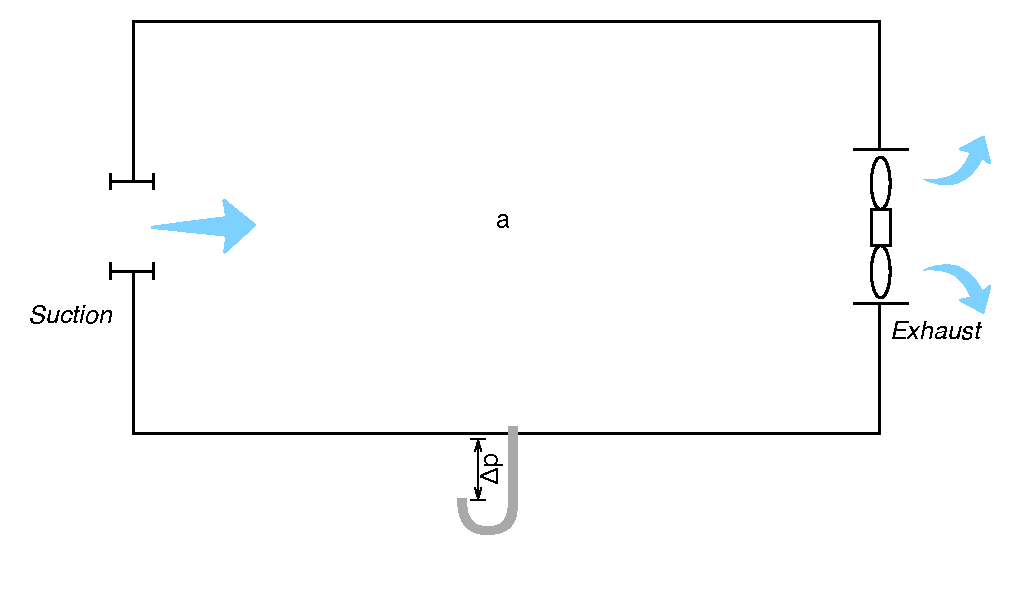
\includegraphics[width=8cm,clip]{chamber.eps}
\end{center}
\end{minipage}
\begin{minipage}{0.45\hsize}
\begin{center}
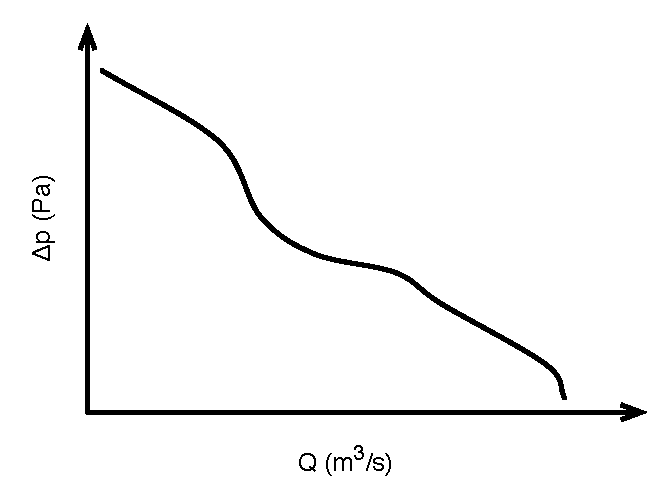
\includegraphics[width=6cm,clip]{fan-PQ.eps}
\end{center}
\end{minipage}
\caption{チャンバーによるファンの特性測定とP-Q線図.}
\label{fig:chamber&p-q}
\end{figure}

こうして得られたファンのP-Q特性を計算に用いる場合には,次の点に注意する必要がある.合わせて,CBCソルバーの実装方針も記す.
\begin{enumerate}
\item ファンの直近にある物体の影響\\
 ファン近傍に物体がある場合には,測定時の状況とはP-Q特性が異なるために適用には注意が必要となる.基本的にはファン前後の近距離には物体を配置しないことであるが,シュラウドのようにほぼ一体となっているものは,シュラウド込みで測定し,P-Q特性を取得するという利用方法も考えられる.
\vspace{2mm}

\item ラム圧の影響\\
 自動車の車載ファンのように走行風がある場合や,流路の狭い部分に設置されたファンの場合には,動圧の影響が無視できない.
この場合,動圧分の補正をしないとファンの動作点がずれていく.
計算モデルにおけるファン部分の上流側,下流側の位置をそれぞれ1,2で表し,静圧,動圧,全圧をそれぞれ$p_S,\,p_D,\,p_T\, (p_T = p_S + p_D)$とする.
圧力ゲインの計算方法として,測定データに基づく実装として,次の2通りが考えられる\footnote{ファン下流の速度が得られている場合には,$p_{T2}$を用いた方法も考えられるが,一般的な測定データとしては得られない.}.
\begin{enumerate}
\item ファン前後の静圧差で計算する.つまり,$\Delta p = p_{S2} - p_{S1}$.この実装では,動圧の影響を考慮できずに動サテンがずれる.
\item 上流側の全圧と下流側の静圧の差で計算する.つまり,$\Delta p = p_{S2} - p_{T1}$.この実装により,上流側の動圧の影響を取り込むことができる.
\end{enumerate}
CBCでは(b)の実装を行う.
\vspace{2mm}

\item 測定値の反映\\
計算では測定データを多項式近似によりモデル化する方法が採られる.一般的には,P-Q特性を一次式で近似することが多いが,一次式に乗らない点の影響が大きな場合がある.これは,多項式近似をしても根本的にはなくならない.そこで,CBCでは測定データ点をそのままテーブルとして保持し,データテーブルをピックアップしてP-Q特性を計算する.実装としては,\hyperlink{tgt:DH}{DataHolderクラス}を用いる.
\vspace{2mm}

\item 回転数や風量によるP-Q特性の補正\\
P-Q特性は定格回転数のみで有効である.回転数が異なる場合には補正したデータを用いる必要がある.
\[
\begin{array}{ll}
\vspace{2mm}
風量比  & \displaystyle{ \frac{Q_2}{Q_1} \,=\, \left( \frac{L_2}{L_1} \right)^3 \,\frac{N_2}{N_1} }\\
静圧比  & \displaystyle{ \frac{P_2}{P_1} \,=\, \left( \frac{L_2}{L_1} \right)^2 \,\left( \frac{N_2}{N_1} \right)^2 } \\
\end{array}
\]

ここで,$Q,\,L,\,N,\,P$はそれぞれ流量,ファンブレード径,回転数,静圧を表し,1,2は状態を表す.

\end{enumerate}


%
\subsubsection{旋回流}
ファンの軸流方向についてはP-Q特性でその流量(速度成分)が与えられるが,回転方向成分は何らかのモデルが必要となる.
よく使われる方法として,スリップ率を与える方法がある.スリップ率を一様に与える方法や半径方向の分布を与える方法などバリエーションは考えられるが,まず一様に与える方法を採用する.

ファンの通過風速については,流路面積を考慮する必要がある.つまり,ファンのボス部分は有効な通過面積ではないため,この部分の面積を除いた断面積を流路面積として扱う.これにより,同じ流量でも通過風速が異なり,動圧に反映され,P-Q特性のルックアップ値が異なるため,注意する.

熱解析の場合には,ファンボス部分の背後に設置されているモータが発熱体として指定されることもある.

さらに,ファン停止時には逆流も許すように流路部分がフリーとなるように考える.これは,外力項をゼロにすることで対応する.




%
\subsubsection{実装と解法の手順}


%
\subsubsection{遠心ファン}
遠心ファンでは,吸入部分と排気部分で流速の方向が異なり,上記の軸流タイプの実装ができない.
そこで,吸入部分と排気部分の速度ベクトルを規定し,圧力差をP-Q線図により与える実装とする.




\pagebreak
%
\subsection{多孔質体モデル}
\label{sec:porous model}
本節では,多孔質モデルの取り扱いについて説明する.

\subsubsection{Darcyモデル}

均質な空間に$A^{\prime}\,[m^2]\,\times\,L^{\prime}\,[m]$の直方体の検査体積を考える.両端の圧力差が$\Delta P^{\prime} \,[Pa]$で流量が$Q^{\prime}\,[m^3/s]$の場合,透過率(Permeability)を$k\,[m^2]$として,
\begin{equation}
Q^{\prime} \,=\, k \frac{A^{\prime}}{\mu} \frac{\Delta P^{\prime}}{L^{\prime}}
\label{Darcy's law 1}
\end{equation}

\begin{equation}
u^{\prime} \,=\, \frac{Q^{\prime}}{A^{\prime}} \,=\, \frac{k}{\mu} \frac{\Delta P^{\prime}}{L^{\prime}}
\label{Darcy's law 2}
\end{equation}

ここで,$\mu\,[Pa \cdot s]$は粘性係数,$u^{\prime}\,[m/s]$は見かけの通過流速(多孔質内の平均速度)である.$\Delta P^{\prime}/L^{\prime}$は圧力勾配なので,$u^{\prime}\,(\mu/k)$が力を表す.したがって,多孔質体部分の存在により流体に作用する外力は,

\begin{equation}
{F_{D}}_{\,i}^{\prime} \,=\, - {u_{i}}^{\prime} \frac{\mu}{k}
\label{NS_darcy_force}
\end{equation}

\textbf{式(\ref{NS_ext_force ND})}の形式に合わせて,$\rho^{\prime} {u_{0}^{\prime}}^{2}/L^{\prime}$で無次元化すると,

\begin{equation}
{F_{D}}_{\,i} \,=\, - \frac{1}{K}{u_{i}}
\label{NS_darcy_force_ND}
\end{equation}

ここで,$K$は無次元透過率を表す.
\begin{equation}
K \,=\, \frac{k}{\mu} \frac{\rho^{\prime} {u_{0}}^{\prime}}{L^{\prime}}
\label{permeability ND}
\end{equation}


\subsubsection{軸方向の異方性を考慮したDarcyモデル}

非等方性を考慮したDarcyモデルは\textbf{式(\ref{permeability aniso})}のように表せる.

\begin{equation}
{F_{D}}_{\,i}^{\prime} \,=\, - \frac{\mu}{k_{ji}}{u_{j}}^{\prime}
\label{permeability aniso}
\end{equation}

$k_{ji}$は異方性の係数を表すテンソルであるが,ここでは主軸方向の非等方性のみを考えるので,

\begin{equation}
k_{i} \,=\, 
\begin{pmatrix}
k_{1} & 0 & 0\\
0 & k_{2} & 0\\
0 & 0 & k_{3}
\end{pmatrix}
\label{permeability matrix}
\end{equation}

\textbf{式(\ref{permeability ND})}と同様に無次元化すると,

\begin{equation}
{F_{D}}_{\,i} \,=\, - \frac{1}{K_{i}} {u_{i}}
\label{NS_darcy aniso ND}
\end{equation}

Darcyモデルを用いる場合に必要なパラメータは\textbf{式(\ref{permeability matrix})}の主軸方向の成分となる.等方性の場合には,係数$k_{1},\,k_{2},\,k_{3}$に同じ値を与える.パラメータの記述については,\textbf{\ref{Darcy model param}}を参照.


%
\subsection{共通の前処理}
圧力損失,ファン,多孔質体の各境界条件は,基礎方程式の外力項としてモデル化されている.
この外力項は各コンポーネントの体積占有率の情報を必要とする.
しばしば設計で用いられる不完全な入力形状データからコンポーネントの占有率を計算することは,内外判定に曖昧さが生じるため少々厄介である.
また,マクロモデルは実際の詳細な形状があったとしても,計算のために少々形状変更を行う必要もある.
そこで,モデルの特性と前処理のバランスを考慮して,以下の方針でモデル化し前処理を行う.

\begin{enumerate}
\item コンポーネントを矩形や円筒形に近似したボリュームとして扱い,体積占有率を自動計算する,
\vspace{2mm}

\item ボリュームを再現する幾何情報は数値データとして入力する.
幾何情報データをCADデータから読み取る作業は手間がかかるが,V-Xgenの機能として実装することも可能.
svx/sbx出力により,設定した占有率をV-Xgenで確認する.
SVの場合にはボクセライズ時の内部データ構造に関係なく,直交等間隔となるので問題ないが,Octreeの場合にはダミーSTLを作成し,格子を細かくしておく必要がある.
\end{enumerate}

%
\subsubsection{入力幾何形状情報}
コンポーネントの幾何形状情報は\textbf{図\ref{fig:geometry_info}}に示すように,圧力損失部とファンのボリュームを構成する情報となる.
\begin{itemize}
\item 圧力損失部
{\small
\begin{equation}
\left.
\begin{array}{lll}
W  & 幅  &  [m] \\
H  & 高さ  & [m] \\
D  & 厚さ  & [m] \\
\overrightarrow{n} & 流出方向法線ベクトル成分 & [-] \\
O_R & 前面の中心座標 & [m] \\
\end{array} \hspace{1cm} \right\}
\end{equation}
}

\item ファン
{\small
\begin{equation}
\left.
\begin{array}{lll}
R_F  & ブレード半径  &  [m] \\
R_B  & ボス半径  & [m] \\
D  & 厚さ  & [m] \\
\overrightarrow{n} & 流出方向法線ベクトル成分 & [-] \\
O_F & 前面の中心座標 & [m] \\
\end{array} \hspace{1cm} \right\}
\end{equation}
}

\end{itemize}


\begin{figure}[htbp]
\begin{center}
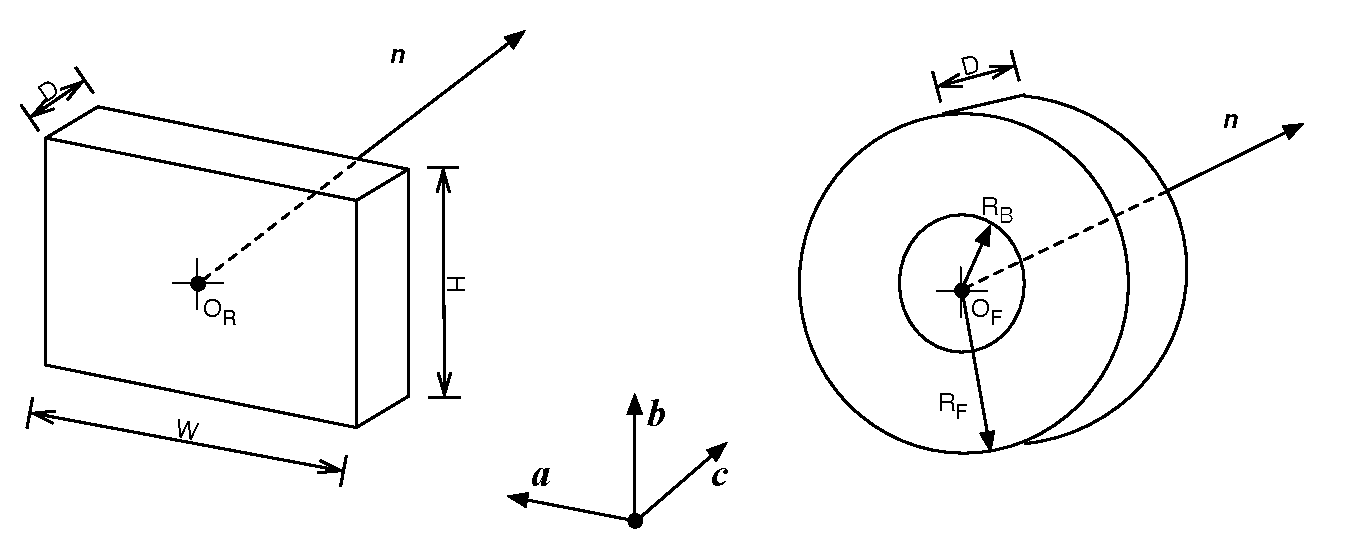
\includegraphics[width=12cm,clip]{compo_dim.eps}
\end{center}
\caption{圧力損失部とファン部の幾何情報.}
\label{fig:geometry_info}
\end{figure}

上記のジオメトリ情報から完全に閉じたボリューム形状を再構築できる.
また,\textbf{図\ref{fig:geometry_info}}の二つの形状は比較的簡単であり,プログラムで内外判定が可能である.

%
\subsubsection{占有率の計算}
コンポーネントの占有率の厳密な計算は難しいため,ある精度でサンプリングすることにより近似的に体積占有率を求める.
また,コンポーネントは空間内に任意の位置・方向で配置されていると処理が煩雑になる.
そこでまず,コンポーネントの法線と座標の$z$軸が一致し,コンポーネント領域が単位立方体になるようにアフィン変換した上で,内外判定を行う.

\paragraph{占有率計算のアルゴリズム}

\begin{enumerate}
\item まず,幾何情報からジオメトリBVのサイズを決定する.ジオメトリBVからインデクススペースのBVを計算する.このとき,外側に1層広げておく.
\item 座標変換を行う.
\item インデクスBVを探索範囲として,セルを構成する8つのノードに対して,内外判定を行う.内側であればラベル\verb|01|,外側の場合にはラベル\verb|00|を割り当てる.ラベルは2ビットを使って判断.
\item ノードの内外判定情報から,セルの内外判定を行う.セルを構成する8つのノードが全て\verb|01|の場合,完全に内部のセル\verb|01|とする.ノードが全て\verb|00|の場合,完全に外側のセル00とする.ラベルが\verb|00|でも\verb|01|でもないセルは\verb|10|のラベルを割り当てる.
\item ラベルが\verb|00|のセルには体積率$\beta=0.0$,ラベル\verb|01|のセルには$\beta=1.0$を与える.
ラベル\verb|10|のセルは,境界面でサブサンプリングの対象になる.
\item サブサンプリングは$5\times5\times5$で行う.三次元の体積で1/125の近似精度となり,8ビット幅で表現可能\footnote{計算時にも量子化した状態からfloatに変換して計算.ロードを減らせる}.
\end{enumerate}

\begin{figure}[htdp]
\begin{minipage}{0.5\hsize}
\begin{center}
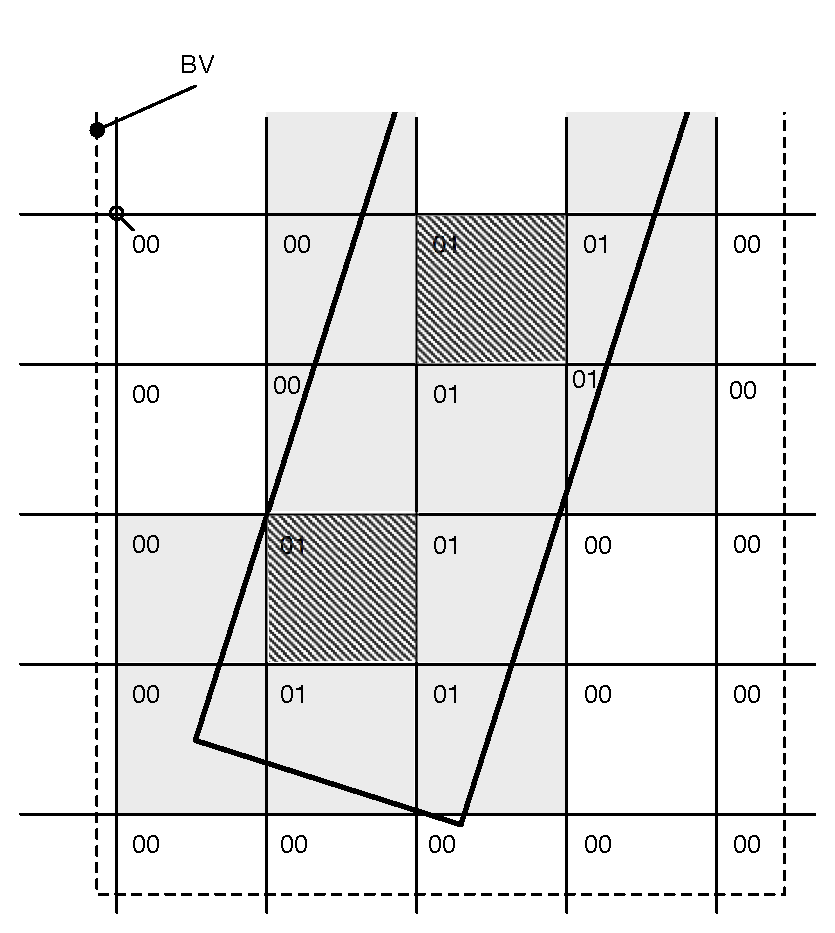
\includegraphics[width=7cm,clip]{compo_BVH.eps}
\end{center}
\end{minipage}
\begin{minipage}{0.45\hsize}
\begin{center}
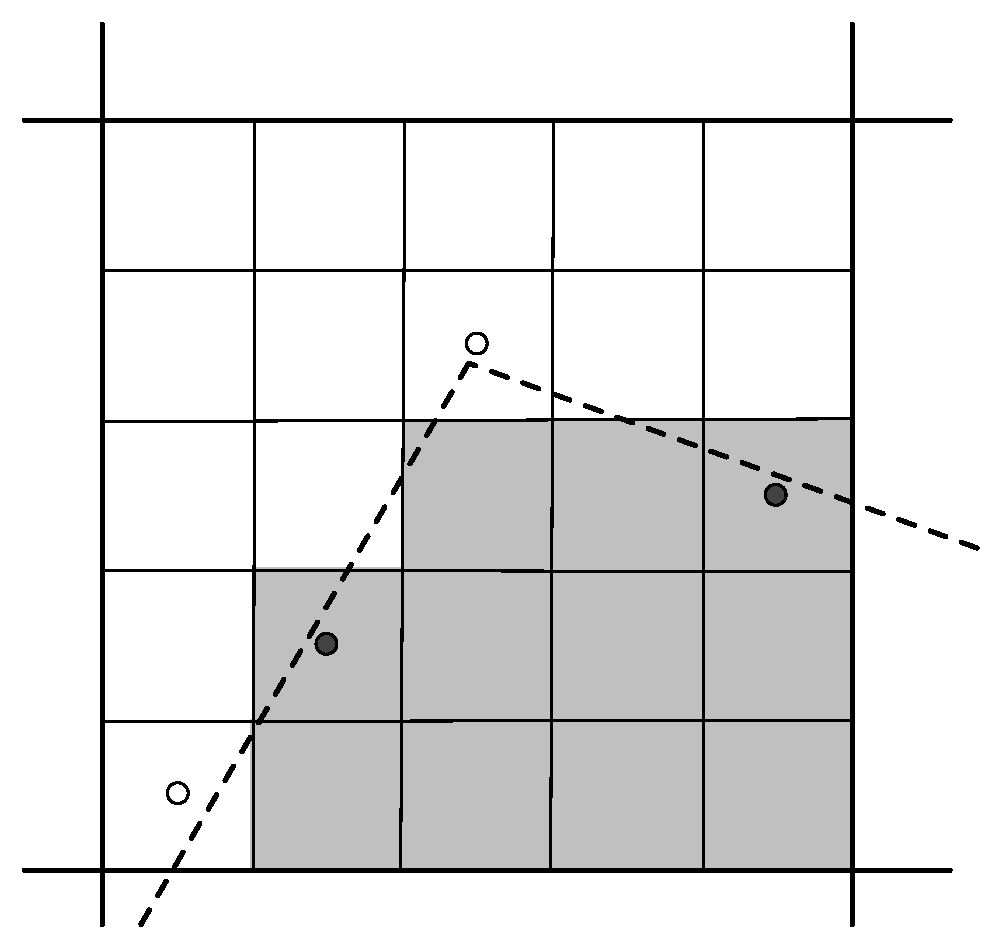
\includegraphics[width=6cm,clip]{subsampling.eps}
\end{center}
\end{minipage}
\caption{占有率の計算は,ノードにラベリングし(ノードの右下位置にラベルを表示),サブサンプリングする要素を特定する.グレー部分がサブサンプリング対象で,ハッチング部分は完全に内部にあるセル.サブサンプリングでは,セルセンタ位置でサンプリングを行い,占有率を計算する.右図は二次元の場合で,11/25の占有率となる.}
\label{fig:sub-sampling}
\end{figure}

%
\paragraph{アフィン変換}
コンポーネントの形状は,空間内の任意の位置に存在する.また,その配置は格子に沿うとは限らない.
そこで内外判定を簡単にするため,コンポーネントの法線$\overrightarrow{n}$と座標の$z$軸方向の単位ベクトルが一致するように,コンポーネントBVの矩形領域をアフィン変換し,単位領域にマッピングする.
さらに,点$O_R$と原点を一致させるように平行移動する.
この座標変換により,コンポーネントのBVは\textbf{図\ref{fig:compo transform}}のようになる.

\begin{figure}[htdp]
\begin{minipage}{0.45\hsize}
\begin{center}
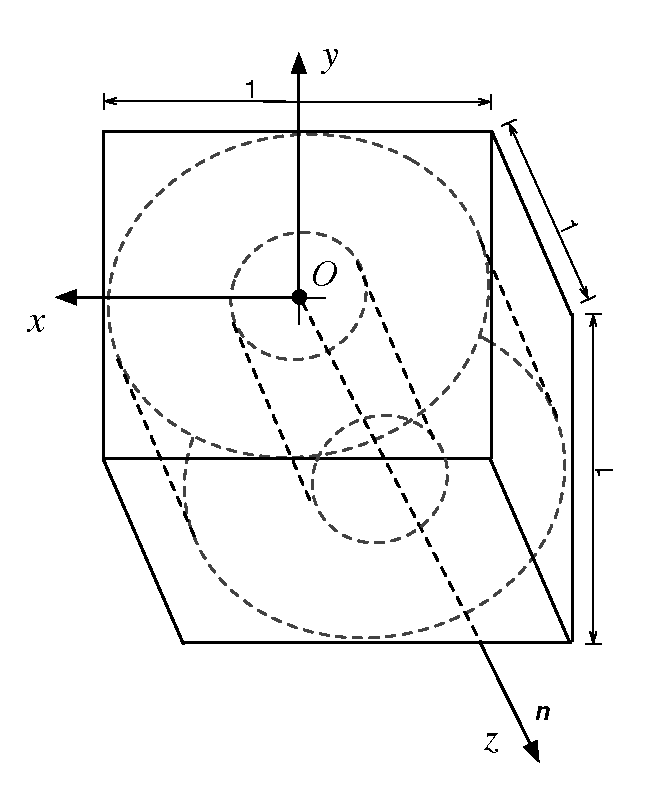
\includegraphics[width=6.5cm,clip]{compo_trnsfm.eps}
\end{center}
\end{minipage}
\begin{minipage}{0.5\hsize}
\begin{center}
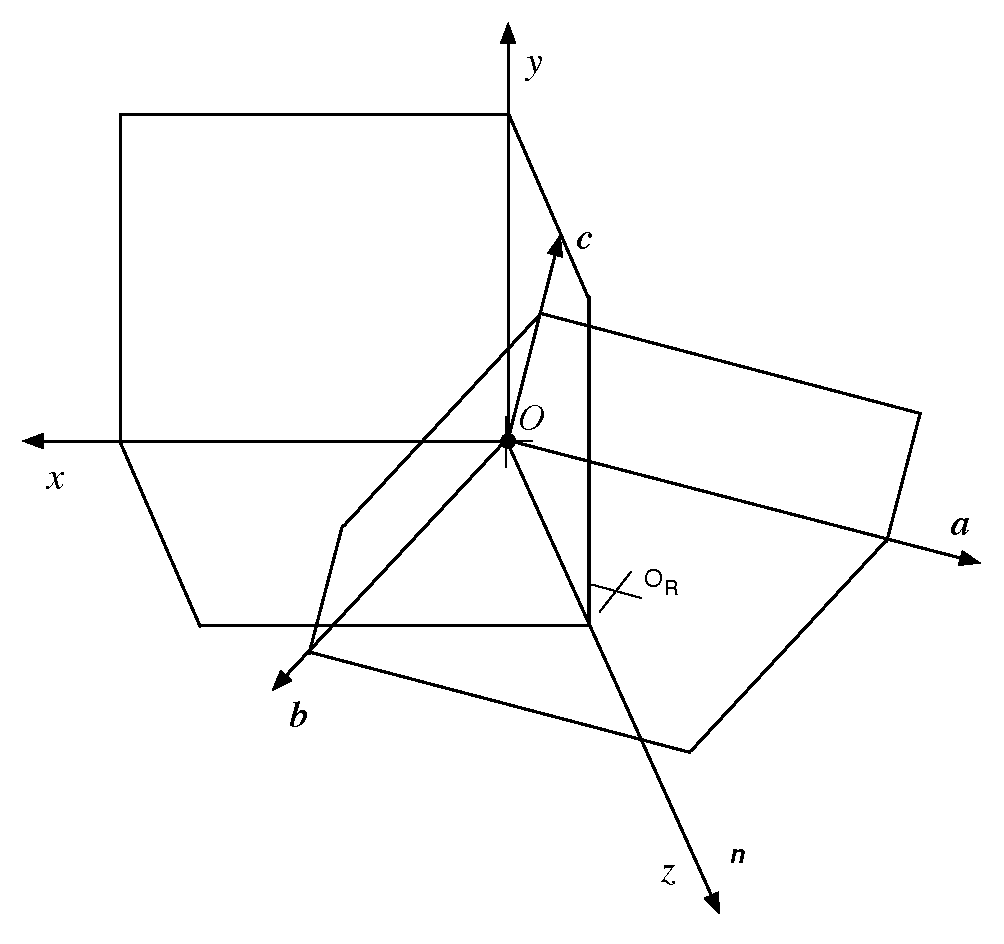
\includegraphics[width=8cm,clip]{Transform.eps}
\end{center}
\end{minipage}
\caption{コンポーネントのアフィン変換.任意の配置から,単位立方体へマッピングする.局所基底の取り方は,流出方向が$\bm c$となるようにする.}
\label{fig:compo transform}
\end{figure}

\begin{enumerate}
\item Appendixに示す\hyperlink{tgt:affin}{アフィン変換}の準備のために,\textbf{図\ref{fig:geometry_info}}の局所座標の基点を原点に平行移動し,\textbf{図\ref{fig:compo transform}}の右図のように配置する.
コンポーネントの局所座標の取り方は,\textbf{図\ref{fig:geometry_info}}の$(\bm a,\, \bm b,\, \bm c)$のように取る.
まず,法線ベクトル$\bm c$を流出方向にとり,それと直交する補助ベクトル$\bm a,\, \bm b$を右手系になるように取る.
\item このとき,変換行列の各成分は\textbf{式(\ref{eq:coef-before})}となる.
\item $O_R$を原点に重ねるように平行移動し,\textbf{図\ref{fig:compo transform}}の左図になるようにする.
\end{enumerate}


%
\paragraph{内外判定}
内外判定は,矩形領域の場合には単位立方体内にあるかどうかの判定,ファンの場合には$xy$平面でブレード部にあるかどうかを見て,奥行き方向に1の範囲に収まっているかで判定する.

%
\paragraph{サブサンプリング}
対象となるセルに対して,$5^3$のサブセルを想定し,サブセルのセルセンター位置でサンプリングを実行する.
オリジナルの空間座標でサンプリング点を求め,それを座標変換して内外判定を行う.

\pagebreak
%
\section{Immersed Boundary}
\label{sec:Immersed Boundary Method}
Immersed Boundary Methodの中でDirect Forcingとして知られる方法\cite{Yusof:97:CTR-ARB}を実装する.これは,指定した速度成分を指定セルに与える境界条件である.Navier-Stokes方程式に強制力を表す外力項${F_{DF}}_{i}$を導入する.

\begin{equation}
\begin{array}{l}
\displaystyle{
{\frac{\partial u_{i}}{\partial t}}^{n+1} 
\, =\, H_{i}
- {\frac{\partial p}{\partial x_{i}}}^{n+1} + {F_{DF}}_{i}
}\\
\displaystyle{
H_{i} \,=\, - \frac{\partial}{\partial x_{j}} \left({ u_{i} u_{j} }\right)
+ \frac{1}{Re} \frac{\partial}{\partial x_{j}} 
\left({ \frac{\partial u_{i}}{\partial x_{j}} + \frac{\partial u_{j}}{\partial x_{i}} }\right) 
}
\end{array}
\label{NS_IB ND}
\end{equation}

${F_{DF}}_{i}$は${u_{i}}^{n+1}=u_{i}^{T}$を満足するように与えられる,つまり,

\begin{equation}
{F_{DF}}_{i} \,=\, - H_{i} 
+ {\frac{\partial p}{\partial x_{i}}}^{n+1}
+ \frac{u_{i}^{T} - u_{i}^{n}}{\Delta t}
\label{Direct forcing term}
\end{equation}

これは,速度ベクトルに,次ステップで指定したい速度${u_{i}}^{T}$を代入することで実装できる.
この外力の導入により,強制した部分の連続の式にソース項$S_{DF}$が同時に導入される.したがって,Poisson反復の収束判断には速度の発散値の指標を用いない方が良い.ただし,$S_{DF}$の値は経験上,収束閾値よりも大きいが小さな値にとどまることが多い.

\begin{equation}
{\frac{\partial u_{i}}{\partial x_{i}}}^{n+1} \, =\, S_{DF}
\label{Cont_IB_src ND}
\end{equation}

Fractional Step法による解法の手順を示すと,
\begin{enumerate}
\item Pseudo vector
\begin{equation}
\begin{array}{ll}
\displaystyle{ \frac{{u_{i}}^{*} - {u_{i}}^{n}}{\Delta t} \,=\, {H_{i}}^{n} } & (1st\,Order)\\
\displaystyle{ \frac{{u_{i}}^{*} - {u_{i}}^{n}}{\Delta t} \,=\, \frac{3}{2}{H_{i}}^{n} - {H_{i}}^{n-1} } & (2nd\,Order)
\end{array}
\label{DF pesudo}
\end{equation}

\item Poisson
\begin{equation}
\frac{\partial}{\partial x_{i}} {\frac{\partial P}{\partial x_{i}}}^{n+1} \,=\, 
\frac{1}{\Delta t} {\frac{\partial u_{i}}{\partial x_{i}}}^{*}
\label{DF Poisson}
\end{equation}

\item Projection
\begin{equation}
\frac{{u_{i}}^{**} - {u_{i}}^{*}}{\Delta t} \,=\, - \frac{\partial}{\partial x_{i}} {\frac{\partial P}{\partial x_{i}}}^{n+1}
\label{DF Projection}
\end{equation}

\item Forcing
\begin{equation}
\begin{array}{l}
\displaystyle{ \frac{{u_{i}}^{n+1} - {u_{i}}^{**}}{\Delta t} \,=\, {F_{DF}}_{i} }\\
\displaystyle{ {F_{DF}}_{i} \,=\, \frac{{u_{i}}^{T} - {u_{i}}^{**}}{\Delta t} }
\end{array}
\label{DF forcing}
\end{equation}
このステップでは,指定領域内部の速度定義点に所望の速度${u_{i}}^{T}$を強制する.

\end{enumerate}

%
\begin{comment}
\section{sec:開口率モデル}
開口率モデルでは,指定されたセルの表面の開口面積を指定する.単独,あるいは多孔質体モデルと組み合わせても利用可能である.
\textbf{式(\ref{FVM:NS})}と\textbf{式(\ref{FVM discrete:NS})}を参考に,対流項のみを有限体積的に考える.セル幅を$h$とすると,

\begin{equation}
\frac{\partial \boldmath{u}}{\partial t} 
\,=\, 
- \frac{1}{V} \sum\limits_{i} { \boldmath{uu}_{i} \cdot \boldmath{n}_{i} \hspace{0.3em} \Delta s_{i} }
\,=\,
- \frac{1}{V} \sum\limits_{i} { \boldmath{uu}_{i} \cdot \boldmath{n}_{i} \hspace{0.3em} A_{i}\, h^{2}}
\label{Area Fraction NS}
\end{equation}

ここで$A_{i}$はセルのi番目のフェイスの開口率である.開口率の定義は,\textbf{図\ref{area def}}に示すように,流動に有効な面積をセル幅を基準にした無次元パラメータであり,二次元の場合には\textbf{式(\ref{open rate})}で定義する.

\begin{equation}
A \,=\, \frac{h_{a}}{h} \qquad [-]
\label{open rate}
\end{equation}


一旦,対流流束を計算した後,開口率が定義されている部分のみに開口率を乗じて流束を制限することにより,セル界面での閉塞効果を導入する.

\begin{figure}[htbp]
\begin{center}
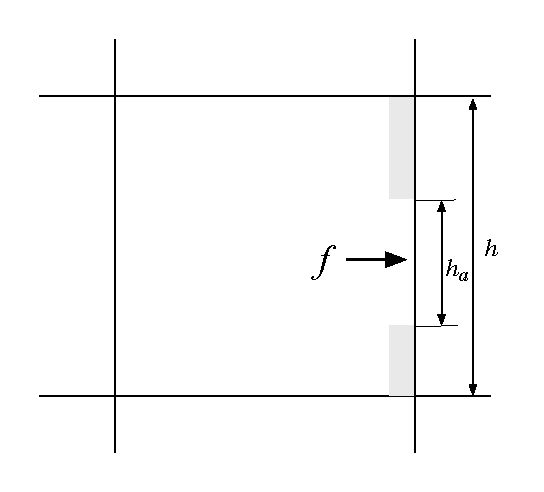
\includegraphics[width=6.5cm,clip]{AreaFraction.eps}
\end{center}
\caption{開口率の定義}
\label{area def}
\end{figure}

\end{comment}













%
\chapter{境界条件と媒質設定}
\begin{abstract}
本章では,CBCソルバークラスで設定できる境界条件と媒質情報の設定について説明する.まず境界条件と媒質を指定するXMLタグの構造について述べた後,流れと熱の境界条件について説明する.\ref{chpt:ebcs}章で説明したDirichlet型とNeumann型の基本的な境界条件を用いた物理的な境界条件について述べる.また,パラメータの設定については\ref{chpt:m_medium}章で詳しく説明する.
\end{abstract}
\graphicspath{{./fig_BC/}}

%
\section{パラメータとXML構造}

%
\subsection{CBCソルバークラスで指定する境界条件と媒質のパラメータ}

境界条件はBC\_Tableセクション,媒質パラメータはMedium\_Tableセクションに記述する.

\begin{itemize}
\item BC\_Table
	\begin{itemize}
	\item InnerBoundary
	\item OuterBoundary
	\begin{itemize}
		\item Basic\_BCs
		\item Face\_BC
	\end{itemize}
	\end{itemize}
\item Medium\_Table
	\begin{itemize}
	\item Fluid
	\item Solid
	\end{itemize}
\end{itemize}

%
\subsection{BC\_Tableセクションの構造と境界条件}
境界条件を記述するBC\_Tableセクションは,SphereConfig\index{SphereConfig}内に記述しても良いし,独立したファイルに記述しても良い.独立ファイルとして扱う場合には,DomainInfo\index{DomainInfo}セクションで次のように外部ファイルとして記述しておく.

\begin{indentation}{3zw}{0zw}
\small
\begin{program}
<Param name="BCTBL" dtype="STRING" value="xml/boundary.xml"/>
\end{program}
\noindent valueには,sphereを起動するディレクトリからの相対パスとなるように記述しておく.
\end{indentation}
\vspace{2mm}

\noindent BC\_Tableセクションは,内部境界条件InnerBoundary\index{InnerBoundary}と外部境界条件OuterBoundary\index{OuterBoundary}の2つを記述する.
内部境界条件と外部境界条件の指定は便宜的に分離しているが,コード中では同じ方法で実装している.

%
\subsubsection{OuterBoundary}
計算領域の外部境界条件を記述し,次の方針により指定する.

\begin{enumerate}
\item 候補となる境界条件の種類をBasic\_BCsタグ内にリストアップし,基本リストを作成する.境界条件の基本リスト\index{きほんりすと@基本リスト!きょうかいじょうけんの@境界条件の---}には,ユニークなID(番号)を割り振る.
\item Face\_BCタグ内において,境界条件の基本リストのIDを参照し,計算領域の外部境界の各面における境界条件を指定する.
\end{enumerate}

\noindent 下記の例では,境界条件の候補として,ID=1, 5, 8をリストアップしておき,Xマイナス方向の外部境界面に流入出境界条件(ID=5)を与え,Yマイナス方向の外部境界面に壁面境界条件(ID=1)を与えている.

\begin{indentation}{3zw}{0zw}
{ \small
\begin{program}
<BC_Table>
    <OuterBoundary>
      <Elem name="Basic_BCs">
        <Elem name="Wall" id="1">
          <Param name="Normal_x"      dtype="REAL"   value="0.0" />
          <Param name="Normal_y"      dtype="REAL"   value="0.0" />
          <Param name="Normal_z"      dtype="REAL"   value="0.0" />
          <param name="specified_type"  dtype="string" value="velocity" />
          <Param name="specified_value"    dtype="REAL"   value="0.0" />
          <param name="profile"    dtype="string" value="constant" />
          <param name="heat_type"  dtype="string" value="adiabatic" />
        </Elem>
        <Elem name="traction_free" id="8">
            <Param name="ambient_temperature"    dtype="REAL"   value="20.0" />
        </Elem>
        <Elem name="in_out" id="5">
          <Param name="velocity_type" dtype="STRING" value="minmax" />
          <Param name="ambient_temperature"    dtype="REAL"   value="20.0" />
        </Elem>
      </Elem>
    
      <Elem name="Face_BC">
        <Elem name="X_MINUS" id="5" comment="inout">
          <Param name="Guide_Cell_ID" id="1" />
        </Elem>
        <Elem name="X_PLUS"  id="5" comment="inout">
          <Param name="Guide_Cell_ID" id="1" />
        </Elem>
        <Elem name="Y_MINUS" id="1" comment="wall">
          <Param name="Guide_Cell_ID" id="2" />
        </Elem>
        <Elem name="Y_PLUS"  id="5" comment="inout">
          <Param name="Guide_Cell_ID" id="1" />
        </Elem>
        <Elem name="Z_MINUS" id="5" comment="inout">
          <Param name="Guide_Cell_ID" id="1" />
        </Elem>
        <Elem name="Z_PLUS"  id="5" comment="inout">
          <Param name="Guide_Cell_ID" id="1" />
        </Elem>
      </Elem>
    </OuterBoundary>
</BC_Table>
\end{program}
}
\end{indentation}

境界条件は,\ref{chpt:ebcs}章で説明したようにDirichlet型とNeaumann型のプリミティブな形式で実装されるが,指定は物理的な状態により指定する.
指定できる境界条件の種類を\textbf{表\ref{tbl:outer BC physical}}に示す.熱流れの場合には,壁面境界の場合に細かい指定が可能である.

\begin{indentation}{3zw}{0zw}

\begin{table}[htdp]
\caption{外部境界で指定できる流れと熱の境界条件の種類}
\begin{center}
\small
\begin{tabular}{ll|ll} \toprule
流れの境界指定のキーワード &  流れの境界条件 & 熱境界指定のサブキーワード & 熱境界条件\\ \midrule
In\_Out & 流入出境界 & Ambient\_Temperature & 流入温度指定と対流流出\\
Outflow & 流出境界 & $\leftarrow$ & 対流流出\\
Periodic & 周期境界 & $\leftarrow$ & 周期境界\\
Specified\_Velocity & 流入境界 & Temperature & 流入温度指定\\
Symmetric & 対称境界 & $\leftarrow$ & 対称境界\\
Traction\_Free & 遠方境界 & Ambient\_Temperature & 遠方温度指定\\ \hline
Wall & 壁面境界 & Adiabatic & 断熱指定\\
& & HeatFlux & 熱流束指定\\ 
& & HeatTransfer Type\_S & 熱伝達係数と表面温度から熱伝達を計算\\
& & HeatTransfer Type\_SF & 強制対流の層流・乱流熱伝達境界\\
& & HeatTransfer Type\_SN & 自然対流の乱流熱伝達境界\\
& & HeatTransfer Type\_B & 固体壁からの放熱条件\\
& & IsoThermal & 等温指定\\
\bottomrule
\end{tabular}
\end{center}
\label{tbl:outer BC physical}
\end{table}

\end{indentation}

\pagebreak
%
\subsubsection{InnerBoundary}
計算領域内の境界条件を記述するセクションで,\textbf{表\ref{tbl:tag_ibc}}に示す種類を指定できる.
CBCソルバークラスは,内部境界条件をコンポーネント\index{コンポーネント}として扱う.


\begin{table}[htdp]
\caption{内部境界条件(コンポーネント)の種類}
\begin{center}
\small
\begin{tabular}{lllll} \toprule
タグ & 指定位置 & 計算モード & 実装形式 & コンポーネントの説明\\ \midrule
Specified\_Velocity & セル界面 & 流れ・熱流れ & 対流流束 & 速度指定境界\footnotemark[1]\\
Outflow & セル界面 & 流れ・熱流れ & 対流流束 & 流出境界\\
Periodic & セル界面 & 流れ・熱流れ & 参照値指定 & 部分周期境界\\
%FORCING & Direct ForcingによるImmersed Boundary境界条件\\
Pressure\_Loss & セル要素 & 流れ・熱流れ & 外力項 & 圧力損失部\\
%FAN & ファン\\
%DARCY & ダルシー則\\
Inactive & セル要素 & 流れ・熱流れ & マスク & 不活性化する計算空間内のセルIDを指定\\
Cell\_Monitor & セル要素 & 流れ・熱流れ & - & 物理量のモニター位置の指定\footnotemark[2]\\ \hline
Adiabatic & セル界面 & 熱流れ & 熱流束マスク & 断熱セル指定\\
Direct\_Heat\_Flux & セル界面 & 熱流れ & 熱流束 & 熱流束指定\\
HeatTransfer\_B & セル界面 & 固体伝熱 & 熱流束 & 固体壁からの放熱条件\\
HeatTransfer\_S & セル界面 & 熱流れ & 熱流束 & 熱伝達係数と表面温度により計算\\
%HeatTransfer\_N & セル界面 & 熱 & 熱流束 & 熱伝達形式\\
HeatTransfer\_SF & セル界面 & 熱流れ & 熱流束 & 強制対流の層流・乱流熱伝達境界\\
HeatTransfer\_SN & セル界面 & 熱流れ & 熱流束 & 自然対流の乱流熱伝達境界\\
IsoThermal & セル界面 & 熱流れ & 熱流束 & 等温面指定\\
Heat\_Source & セル要素 & 熱流れ & 外力項 & 吸発熱指定\\
Specified\_Temperature & セル要素 & 熱流れ & 温度指定 & セルの温度指定\\
%Radiation
\bottomrule
\end{tabular}
\end{center}
\label{tbl:tag_ibc}
\end{table}
\footnotetext[1]{INFLOWセクションのステートメントでTemperatureを指定する.}
\footnotetext[2]{Monitorは境界条件ではないが,同じしくみを用いて実装しているので,このセクションに設けている.}

\begin{indentation}{3zw}{0zw}
{ \small
\begin{program}
<BC_Table>
  <InnerBoundary>
      <Elem name="specified_velocity" id="3" comment="inlet">
        <Param name="Normal_x"        dtype="REAL"   value="0.0" />
        <Param name="Normal_y"        dtype="REAL"   value="0.0" />
        <Param name="Normal_z"        dtype="REAL"   value="-1.0" />
        <param name="specified_type"  dtype="string" value="velocity" />
        <Param name="specified_value" dtype="REAL"   value="2.0" />
        <Param name="def_face"        dtype="INT"    value="10" />
        <param name="profile"         dtype="string" value="harmonic" />
        <Param name="frequency"       dtype="REAL"   value="2.0" />
        <Param name="initial_phase"   dtype="REAL"   value="0.0" />
        <Param name="constant_bias"   dtype="REAL"   value="0.0" />
        <Param name="temperature"     dtype="REAL"   value="35.0" />
      </Elem>
  </InnerBoundary>
</BC_Table>
\end{program}
}
\end{indentation}

内部境界条件は,外部境界面を除く計算領域内において,セルIDにより指定する.同時に,XMLのInnerBoundaryセクションのID番号にその境界条件の属性を記述する.また,内部境界条件で指定する各コンポーネントの個数と実際の解析モデル中のコンポーネントの個数およびID番号の属性情報は一致している必要がある.
\textbf{指定できる内部境界条件の数は30個が上限}で,
\textbf{指定境界条件数と媒質数の和は63個以下}となる\footnote{これらの制限は,境界条件を効率よく実装する方法の制約から来るもの.}.
Cell\_Monitorは境界条件ではないが,同じ仕組みを用いて実装しているのでこのセクションに設けている.

一方,外部境界条件は,計算領域を構成する外部境界面の各面で同じ境界条件とし,XMLパラメータにより指定する.

%
\subsection{Medium\_Tableセクションの構造}
Medium\_Tableセクションには,\textbf{表\ref{tbl:MTLentry}}に示すように媒質ID\index{ばいしつあいでぃ@媒質ID}の物性値\index{ぶっせいち@物性値}を記述できる.
ここで記述する媒質の基本リスト\index{きほんりすと@基本リスト!ばいしつの@媒質の---}は,解析に利用される候補である.
各媒質は,固体と流体によって記述しなければならない物性値が異なり,指定できる項目を\textbf{表\ref{tbl:material description}}に示す.\\

\begin{indentation}{3zw}{0zw}
{ \small
\begin{program}
<Medium_Table>
  <Elem name="Fluid" id="1" comment="VirtualFluid">
    <Param name="density" dtype="REAL" value="1.0" />
    <Param name="specific_heat" dtype="REAL" value="1.0" />
    <Param name="thermal_conductivity" dtype="REAL" value="1.0" />
    <Param name="kinematic_viscosity" dtype="REAL" value="1.0" />
    <Param name="viscosity" dtype="REAL" value="1.0" />
    <Param name="sound_of_speed" dtype="REAL" value="1.0" />
    <Param name="volume_expansion" dtype="REAL" value="0.04e-3" />
  </Elem>
  <Elem name="Solid" id="600" comment="Fe">
    <Param name="density" dtype="REAL" value="7870.0" />
    <Param name="specific_heat" dtype="REAL" value="442.0" />
    <Param name="thermal_conductivity" dtype="REAL" value="80.3" />
  </Elem>
</Medium_Table>
\end{program}
}

\begin{table}[htdp]
\small
\caption{Medium\_Tableに記述するパラメータ}
\begin{center}
\begin{tabular}{ll} \toprule
XMLキーワード & 説明\\ \midrule
Elem name & Fluid または Solid\\
ID & 媒質ID\\
commnet & 媒質名\\ \bottomrule
\end{tabular}
\end{center}
\label{tbl:MTLentry}
\end{table}


\begin{table}[htdp]
\small
\caption{Medium\_Tableにおける物性値の指定}
\begin{minipage}{.45\textwidth}
\begin{center}
\begin{tabular}{lll}\\ \toprule
Fluidのキーワード & 説明 & 単位\\ \midrule
Density & 密度 & $[kg/m^3]$\\
Specific\_Heat & 定圧比熱 & $[kJ/(kg K)]$\\
Thermal\_Conductivity & 熱伝導率 & $[W/(m K)]$\\
Kinematic\_Viscosity & 動粘性係数 & $[m^2/s]$\\
Viscosity & 粘性係数 & $[Pa/s]$\\
Sound\_of\_Speed & 音速 & $[m/s]$\\
Volume\_Expansion & 体膨張率 & $[1/K]$\\ \bottomrule
\end{tabular}
\end{center}
\end{minipage} \hfill
\begin{minipage}{.45\textwidth}
\begin{center}
\begin{tabular}{lll}\\ \toprule
Solidのキーワード & 説明 & 単位\\ \midrule
Density & 密度 & $[kg/m^3]$\\
Specific\_Heat & 定圧比熱 & $[kJ/(kg K)]$\\
Thermal\_Conductivity & 熱伝導率 & $[W/(m K)]$\\ \bottomrule
\end{tabular}
\end{center}
\end{minipage}
\label{tbl:material description}
\end{table}

\end{indentation}

\pagebreak
%
\section{流れ解析の境界条件}
\label{sec:flow_condition}
本節では,非圧縮性流体の流れの境界条件,つまり速度と圧力の境界条件について説明する.
計算領域とコロケート変数配置\index{へんすうはいち@変数配置!コロケート@Collocated---}の変数のインデクス\index{インデクス}の表記を\textbf{図\ref{fig:index_domain}},\textbf{図\ref{fig:index_cc}}に示す.

\begin{figure}[htdp]
  \begin{center}
  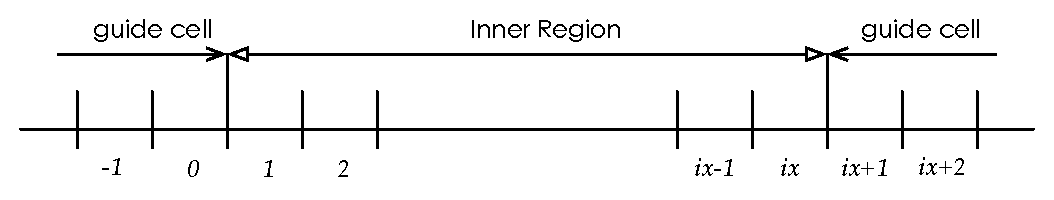
\includegraphics[width=12cm,clip]{index_domain.eps}
  \end{center}
  \caption{計算領域のインデクス}
  \label{fig:index_domain}
\end{figure}

\begin{figure}[htdp]
  \begin{center}
  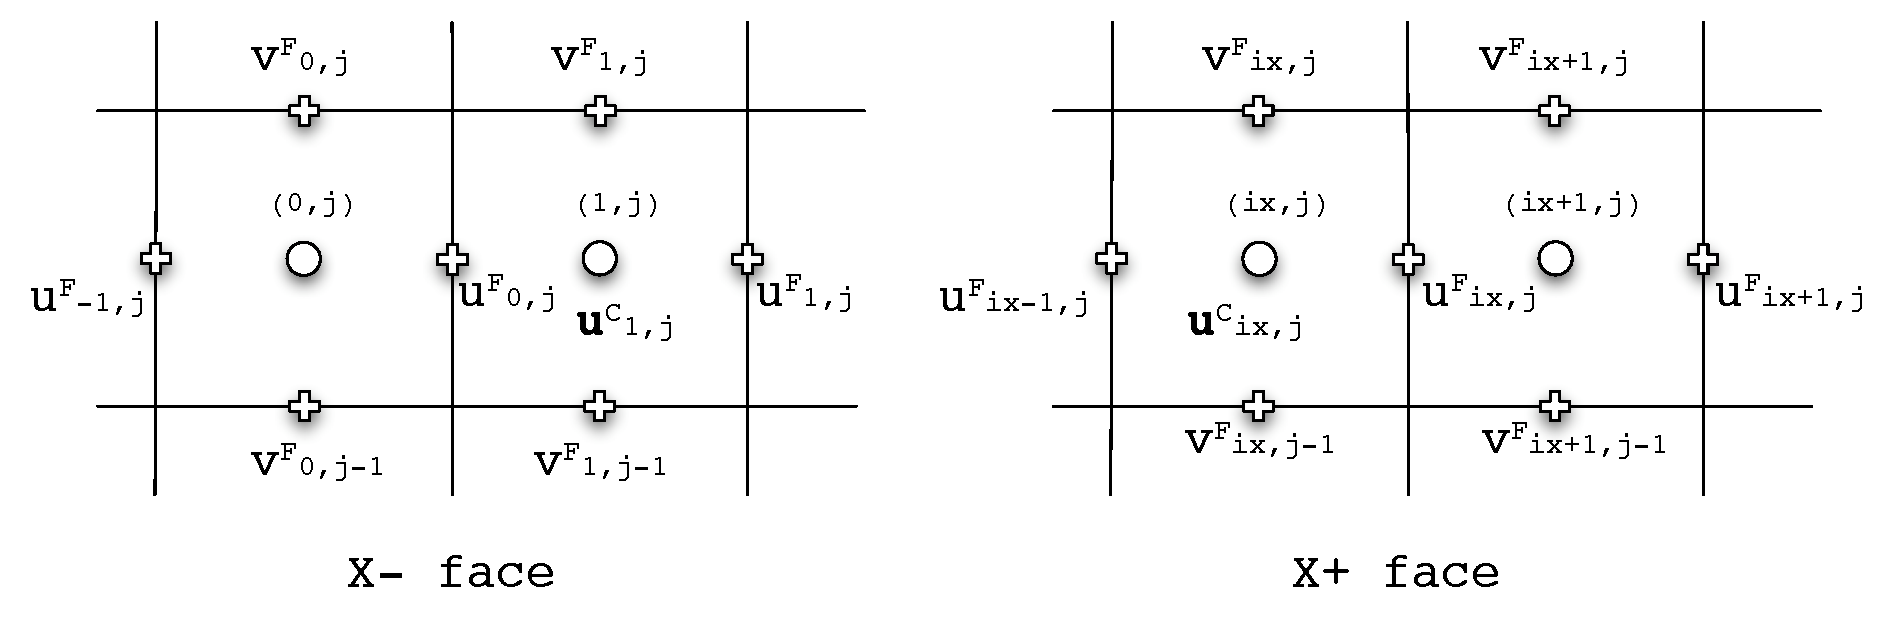
\includegraphics[width=14cm,clip]{index_cc.eps}
  \end{center}
  \caption{コロケート配置の変数のインデクス.基本変数($u_{\,i}^{\,C},\, p,\,\theta$)は全てセルセンタ位置に配置され,補助的な速度ベクトル$u_{\,i}^{\,F}$がスタガード位置に配置される.}
  \label{fig:index_cc}
\end{figure}


%
\subsection{流れの境界条件}
\label{sec:Boundary Conditions}

%
\subsubsection{壁面境界}
\label{sec:BC wall}

\begin{indentation}{3zw}{0zw}
\paragraph{外部境界面}
壁面境界条件は,外部境界条件の場合,XMLパラメータにより指定する.一方,計算領域内部に存在する壁面はセルIDにより指定され,その境界条件はEmbedded Boundary Condition Scheme\textbf{(\ref{sec:EBCS concept})}の仕組みを用いてスキームに組み込まれる.

外部境界は,壁面速度が時間的に変化する場合と固定の場合があり,指定する境界面の移動速度を与える.
ただし,壁面速度ベクトルは壁面と平行なスライド成分のみで,壁面と垂直な成分はゼロである点に注意する.

壁面境界は,Dirichlet型の速度境界条件を用いてセルフェイス位置の運動量流束を直接与える.外部境界では下記のようなXML入力パラメータで指定する.
次の例では,境界条件番号1にz軸に面直でy方向に7[m/s]で移動する壁の境界条件を指定している.

{\small
\begin{program}
<OuterBoundary>
  <Elem name="Basic_BCs">
    <Elem name="wall" id="1">
      <Param name="Normal_x"        dtype="REAL"   value="0.0" />
      <Param name="Normal_y"        dtype="REAL"   value="1.0" />
      <Param name="Normal_z"        dtype="REAL"   value="0.0" />
      <param name="Profile"         dtype="STRING" value="Harmonic" />
      <param name="Specified_Type"  dtype="STRING" value="Velocity" />
      <Param name="Specified_Value" dtype="REAL"   value="7.0" />
      <Param name="Frequency"       dtype="REAL"   value="2.0" />
      <Param name="Initial_Phase"   dtype="REAL"   value="0.0" />
      <Param name="Constant_Bias"   dtype="REAL"   value="0.0" />
    </Elem>
  </Elem>
</OuterBoundary>
\end{program}
}

\noindent 時間的に変化しない壁面境界の場合にはtype=constantを指定する.
時間変化を伴う速度指定はtype=harmonic\_oscillationを指定し,\textbf{式(\ref{eq:harmonic_v})}の形式の単振動\index{たんしんどう@単振動}の境界条件を周期や初期位相,切片(初期振幅)と供に与える\footnote{XMLの例ではコメントアウトされている.}.非定常の場合,振幅はvelocityで与えられる.

\begin{equation}
v \,{=}\, A \sin \left( 2 \mathrm{\pi} ft \,+\, \phi \right) \,+\, b
\label{eq:harmonic_v}
\end{equation}

ここで各パラメータは\textbf{表\ref{tbl:harmonic_table_v_obc}}に対応する.

\begin{table}[htdp]
\small
\caption{速度境界条件の単振動パラメータ}
\begin{center}
\begin{tabular}{lcll} \toprule
XMLキーワード & \textbf{式(\ref{eq:harmonic_v})}中の記号 & 説明 & 単位\\ \midrule
Amplitude & $A$ & 振幅 & $[m/s]$\\
Frequency & $f$ & 周波数 & $[Hz]$\\
Initial\_Phase & $\phi$ & 初期位相 & [rad]\\
Intercept & $b$ & 切片 & $[m/s]$\\ \bottomrule
\end{tabular}
\end{center}
\label{tbl:harmonic_table_v_obc}
\end{table}

計算領域内部の壁面境界条件は,EBCSの仕組みを用いてスキームに組み込まれ,セル界面の流束が指定する壁面速度から直接計算される.
したがって,計算する流体セルからみて,壁面方向に延びるステンシルのセルの値は参照されず不要である.
外部境界の場合には,可視化する場合の利便性を考慮し,出力時にのみガイドセルに値を書き出す.
この場合,境界面を中心に速度勾配一定として,速度成分を外挿する.

\begin{equation}
\left.
\begin{array}{llll}
\vspace{1mm}
\vspace{1mm} x-; & u_{\,0,\,j,\,k}    &=& 2\,u^{\,g} \,-\, u_{\,1,\,j,\,k}\\
\vspace{1mm}     & v_{\,0,\,j,\,k}    &=& 2\,v^{\,g} \,-\, v_{\,1,\,j,\,k}\\
\vspace{3mm}     & w_{\,0,\,j,\,k}    &=& 2\,w^{\,g} \,-\, w_{\,1,\,j,\,k}\\

\vspace{1mm} x+; & u_{\,ix+1,\,j,\,k} &=& 2\,u^{\,g} \,-\, u_{\,ix,\,j,\,k}\\
\vspace{1mm}     & v_{\,ix+1,\,j,\,k} &=& 2\,v^{\,g} \,-\, v_{\,ix,\,j,\,k}\\
\vspace{3mm}     & w_{\,ix+1,\,j,\,k} &=& 2\,w^{\,g} \,-\, w_{\,ix,\,j,\,k}\\

\vspace{1mm} y-; & u_{\,i,\,0,\,k}    &=& 2\,u^{\,g} \,-\, u_{\,i,\,1,\,k}\\
\vspace{1mm}     & v_{\,i,\,0,\,k}    &=& 2\,v^{\,g} \,-\, v_{\,i,\,1,\,k}\\
\vspace{3mm}     & w_{\,i,\,0,\,k}    &=& 2\,w^{\,g} \,-\, w_{\,i,\,1,\,k}\\

\vspace{1mm} y+; & u_{\,i,\,jx+1,\,k} &=& 2\,u^{\,g} \,-\, u_{\,i,\,jx,\,k}\\
\vspace{1mm}     & v_{\,i,\,jx+1,\,k} &=& 2\,v^{\,g} \,-\, v_{\,i,\,jx,\,k}\\
\vspace{3mm}     & w_{\,i,\,jx+1,\,k} &=& 2\,w^{\,g} \,-\, w_{\,i,\,jx,\,k}\\

\vspace{1mm} z-; & u_{\,i,\,j,\,0}    &=& 2\,u^{\,g} \,-\, u_{\,i,\,j,\,1}\\
\vspace{1mm}     & v_{\,i,\,j,\,0}    &=& 2\,v^{\,g} \,-\, v_{\,i,\,j,\,1}\\
\vspace{3mm}     & w_{\,i,\,j,\,0}    &=& 2\,w^{\,g} \,-\, w_{\,i,\,j,\,1}\\

\vspace{1mm} z-; & u_{\,i,\,j,\,kx+1} &=& 2\,u^{\,g} \,-\, u_{\,i,\,j,\,kx}\\
\vspace{1mm}     & v_{\,i,\,j,\,kx+1} &=& 2\,v^{\,g} \,-\, v_{\,i,\,j,\,kx}\\
\vspace{1mm}     & w_{\,i,\,j,\,kx+1} &=& 2\,w^{\,g} \,-\, w_{\,i,\,j,\,kx}\\
\end{array} \qquad \right \}
\label{eq:wall BC velocity}
\end{equation}


壁面境界に対する圧力の境界条件は,Navier-Stokes方程式からNeumann型の圧力境界条件が得られる.つまり,
\begin{equation}
{\frac{\partial p}{\partial x_{\,i}}}^{\,n+1} \,=\, - {\frac{\partial u_{\,i}}{\partial t}}^{\,n+1}
\,-\, \left( u_{\,j}-u_{\,j}^{\,g} \right) \frac{\partial u_{\,i}}{\partial x_{\,j}}
\,+\, \frac{1}{Re} \left( \frac{\partial^{\,2} u_{\,i}}{\partial x_{\,j}^{\,2}} \right)
\label{eq:prs BC from NS}
\end{equation}

\noindent 右辺の空間項は,\textbf{\ref{sec:Algorithm NS}}の各アルゴリズムに応じたタイムレベルで評価する.
レイノルズ数が小さい場合には粘性項の影響が無視できないが,
高レイノルズ数流れにおいては,粘性項の寄与が小さいと仮定し粘性項を省略する場合もある.
\begin{equation}
{\frac{\partial p}{\partial x_{\,i}}}^{\,n+1} \,=\, - {\frac{\partial u_{\,i}}{\partial t}}^{\,n+1}
\,-\, \left( u_{\,j}-u_{\,j}^{\,g} \right) \frac{\partial u_{\,i}}{\partial x_{\,j}}
\label{eq:prs BC from NS for High Re}
\end{equation}

\noindent \textbf{式(\ref{eq:prs BC from NS})},\textbf{(\ref{eq:prs BC from NS for High Re})}は,壁面の時間的・空間的な変化がない場合,

\begin{equation}
{\frac{\partial p}{\partial x_{\,i}}}^{\,n+1} \,=\, 
\frac{1}{Re} \left( \frac{\partial^{\,2} u_{\,i}}{\partial x_{\,i}^{\,2}} \right)
\label{eq:prs BC from NS for Low Re simple}
\end{equation}

\begin{equation}
{\frac{\partial p}{\partial x_{\,i}}}^{\,n+1} \,=\, 0
\label{eq:prs BC from NS for High Re simple}
\end{equation}


\noindent と簡単な形式になる.CBCソルバークラスでは,\textbf{(\ref{eq:prs BC from NS for High Re simple})}の壁面境界条件を用いている.
%\textbf{式(\ref{eq:prs BC from NS for Low Re simple})}
%全計算領域の壁面に対する境界条件として,高レイノルズ数型と低レイノルズ数型のどちらを用いるかをSteerセクションで指定しておく.
%次の例では,高レイノルズ数の場合の勾配ゼロを指定している.
%{ \small
%\begin{program}
%<Param name="Neumann_BCType_of_Pressure_on_solid_wall" dtype="string" value="grad_zero">
%\end{program}
%}

\vspace{5mm}
\paragraph{内部領域}
計算領域内部にある固体部分は,任意に現れる特徴があるので,その表面位置で粘着条件が課されるように対流項や粘性項のスキーム中で処理を行う.
セル界面が固体壁に接するかどうかは,セルの状態を表すビットフィールドからマスクを生成し,その情報を元に流束を計算する.
\end{indentation}

\pagebreak
%
\subsubsection{対称境界}
\label{sec:BC symmetric}

\begin{indentation}{3zw}{0zw}
外部境界にのみ用いられる境界条件で,指定する面が対称面であると仮定する.速度については,面直な成分のみ固体壁と同じで,残りはフリーとする.圧力は勾配がゼロとする.

\begin{equation}
\left.
\begin{array}{llll}
\vspace{1mm} x-; & u_{\,0,\,j,\,k}    &=& 2\,u^{\,g} \,-\, u_{\,1,\,j,\,k}\\
\vspace{1mm}     & v_{\,0,\,j,\,k}    &=& v_{\,1,\,j,\,k}\\
\vspace{1mm}     & w_{\,0,\,j,\,k}    &=& w_{\,1,\,j,\,k}\\
\vspace{3mm}     & p_{\,0,\,j,\,k}    &=& p_{\,1,\,j,\,k}\\

\vspace{1mm} x+; & u_{\,ix+1,\,j,\,k} &=& 2\,u^{\,g} \,-\, u_{\,ix,\,j,\,k}\\
\vspace{1mm}     & v_{\,ix+1,\,j,\,k} &=& v_{\,ix,\,j,\,k}\\
\vspace{1mm}     & w_{\,ix+1,\,j,\,k} &=& w_{\,ix,\,j,\,k}\\
\vspace{3mm}     & p_{\,ix+1,\,j,\,k} &=& p_{\,ix,\,j,\,k}\\

\vspace{1mm} y-; & u_{\,i,\,0,\,k}    &=& u_{\,i,\,1,\,k}\\
\vspace{1mm}     & v_{\,i,\,0,\,k}    &=& 2\,v^{\,g} \,-\, v_{\,i,\,1,\,k}\\
\vspace{1mm}     & w_{\,i,\,0,\,k}    &=& w_{\,i,\,1,\,k}\\
\vspace{3mm}     & p_{\,i,\,0,\,k}    &=& p_{\,i,\,1,\,k}\\

\vspace{1mm} y+; & u_{\,i,\,jx+1,\,k} &=& u_{\,i,\,jx,\,k}\\
\vspace{1mm}     & v_{\,i,\,jx+1,\,k} &=& 2\,v^{\,g} \,-\, v_{\,i,\,jx,\,k}\\
\vspace{1mm}     & w_{\,i,\,jx+1,\,k} &=& w_{\,i,\,jx,\,k}\\
\vspace{3mm}     & p_{\,i,\,jx+1,\,k} &=& p_{\,i,\,jx,\,k}\\

\vspace{1mm} z-; & u_{\,i,\,j,\,0}    &=& u_{\,i,\,j,\,1}\\
\vspace{1mm}     & v_{\,i,\,j,\,0}    &=& v_{\,i,\,j,\,1}\\
\vspace{1mm}     & w_{\,i,\,j,\,0}    &=& 2\,w^{\,g} \,-\, w_{\,i,\,j,\,1}\\
\vspace{3mm}     & p_{\,i,\,j,\,0}    &=& p_{\,i,\,j,\,1}\\

\vspace{1mm} z-; & u_{\,i,\,j,\,kx+1} &=& u_{\,i,\,j,\,kx}\\
\vspace{1mm}     & v_{\,i,\,j,\,kx+1} &=& v_{\,i,\,j,\,kx}\\
\vspace{1mm}     & w_{\,i,\,j,\,kx+1} &=& 2\,w^{\,g} \,-\, w_{\,i,\,j,\,kx}\\
\vspace{3mm}     & p_{\,i,\,j,\,kx+1} &=& p_{\,i,\,j,\,kx}\\
\end{array} \qquad \right \}
\label{eq:symmetric BC}
\end{equation}

次の例では,境界条件番号20に対称境界条件を設定する.
{ \small
\begin{program}
<OuterBoundary>
  <Elem name="Basic_BCs">
    <Elem name="symmetric" id="20"/>
  </Elem>
</OuterBoundary>
\end{program}
}
 
\end{indentation}


\pagebreak
%
\subsubsection{流出境界}
\label{sec:BC outflow}

\begin{indentation}{3zw}{0zw}
\paragraph{外部境界面}
流出境界を指定する場合には,流出方向は既知であり,外部境界面を指定することにより流出方向は決まる.
\textbf{図\ref{fig:outflow BC outer}}はX+方向の流出境界を示している.セル$(ix,\,j)$,セル$(ix+1,\,j)$ともに流体を指定する.
つまり,流出方向の外部領域は流体であるので,ガイドセル領域のIDをFace\_BCセクションで流体要素にしておく.
次の例では,id=20は流体要素である.

{\small
\begin{program}
<Elem name="Face_BC">
  <Elem comment="outflow" id="3" name="X_plus">
    <Param id="20" name="Guide_Cell_ID"/>
  </Elem>
</Elem>
\end{program}
}

\begin{figure}[htbp]
\begin{center}
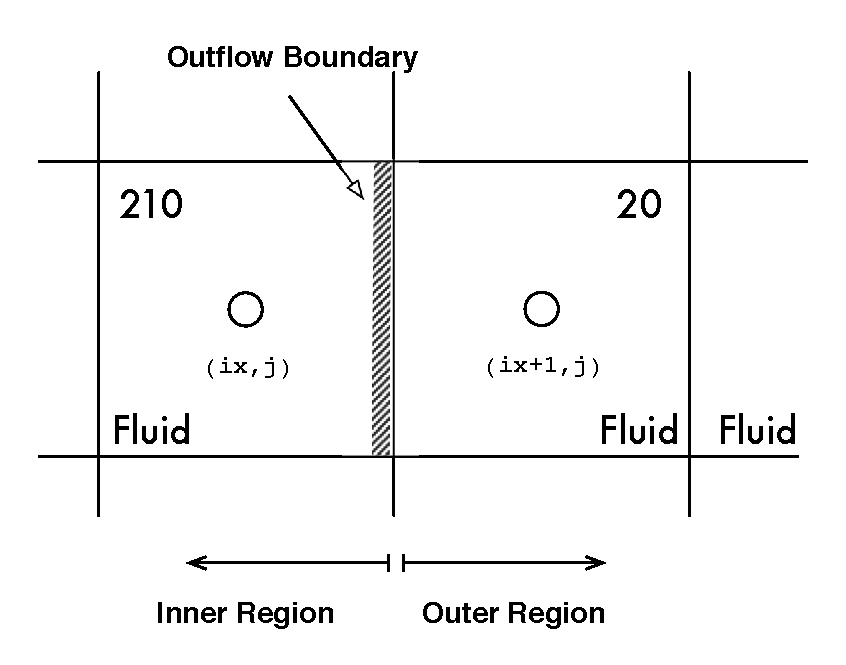
\includegraphics[width=8cm,clip]{outflowBC_outer.eps}
\end{center}
\caption{X+方向の流出境界の設定.}
\label{fig:outflow BC outer}
\end{figure}

次の例では,基本条件として3番に流出境界を登録している.

{\small
\begin{program}
<OuterBoundary>
  <Elem name="Basic_BCs">
    <Elem name="outflow" id="3">
      <Param name="velocity_type" dtype="STRING" value="minmax" />
    </Elem>
  </Elem>
</OuterBoundary>
\end{program}
}

流出境界面における流束は,境界面における流出速度から直接運動量を計算する.\textbf{図\ref{fig:outflow BC outer}}の例は$x$方向の流出面なので対流速度は$x$方向成分,非移流物理量を$\varphi$として,

\begin{equation}
{\left(\, \tilde{f}_i \,\right)}_{\,i+1/2,\,j,\,k} \,=\, {\left( u_{\,1}-u_{\,1}^{\,g} \right)}_{\,i+1/2,\,j,\,k} \,\varphi_{\,i,\,j,\,k}
\label{eq:outflow flux}
\end{equation}

\noindent 流出速度$u_{\,1}$は,セル$(\,i,\,j,\,k\,)$に対する連続の式から求める\footnote{BCvec\_cc.f90 $>$ vibc\_c\_out\_cf\_()}.流出速度は,コンポーネント毎の平均値もしくは最大値と最小値の算術平均を計算している.
流出速度の選び方として,流出断面の平均速度や最大値と最小値の算術平均などが提案されており,外部流や噴流のような無限空間の境界面の場合には,\textbf{式(\ref{eq:minmax outflow})}のMinMaxがよい近似値となる.
流出速度の指定は,Outflow\_Velocity タグにてaverage または minmaxを指定する.
Averageは有効セルの平均値をとる.有効セルは物体でブロックされていないセルである.
MinMaxは,境界面における流速の最大値と最小値の算術平均値を与える.

\begin{equation}
u_{ob} \,=\, \frac{1}{2} \{ max(u_{ob,j,k}) + min(u_{ob,j,k}) \}
\label{eq:minmax outflow}
\end{equation}

粘性項を評価する場合には,セルフェイス面での流出速度から勾配値が次式のように計算される.

\begin{equation}
{\left(\, \frac{\partial \varphi}{\partial x} \,\right)}_{\,i+1/2,\,j,\,k} \,=\, \frac{\varphi_{\,i+1/2,\,j,\,k}-\varphi_{\,i,\,j,\,k}}{h/2}
\label{eq:outflow grad1}
\end{equation}

\noindent コーディングでは格子幅を$h$としているので,勾配値が同じになるように流出速度を修正する\footnote{SetBC3D::modifyViscousEE(), SetBC3D::modifyViscousCN()を参照.\today 現在,この修正は行っていない.}.

\begin{equation}
\varphi_{\,i+1/2,\,j,\,k}^{\,\prime} \,=\, 2\, \varphi_{\,i+1/2,\,j,\,k} \,-\, \varphi_{\,i,\,j,\,k}
\label{eq:outflow grad2}
\end{equation}

\vspace{2mm}

実装としては,流出境界が指定された外部境界面にはBC Index bcv[]にid=31がエンコードされている.したがって,id=31の面に対して,セルセンターの変数に対して,流出境界を考慮した流束計算を行う.具体的には,流出速度が与えられるので,一次風上スキームを適用している\footnote{cbc\_pvec\_vobc(), MUSCLへ変更した方が良い}.


\paragraph{内部領域}
計算内部領域における流出境界は,\textbf{図\ref{fig:outflow BC inner}}のように,グレー部分,つまり$(i,\,j)\sim(i+1,\,j)$セル間の面が流出境界として指定されている.
境界面は,次のように対象となる面を2つのIDで挟むことにより指定する.
キーとなるIDは固体(この例ではid=20)を,def\_faceにid=210を指定し,$i+1/2$面を流出境界としている.
また,指定するid=20の属性は固体で,id=210の属性は流体であること.
加えて,固体セルは2層必要である\footnote{これはMUSCLスキームのステンシル長からの要請であるが,実装は未だupwind}.

{ \small
\begin{program}
<InnerBoundary>
  <Elem name="outflow" id="20" comment="outflow_sec_1">
    <Param name="def_face"      dtype="INT"    value="210" />
  </Elem>
</InnerBoundary>
\end{program}
}

\begin{figure}[htbp]
\begin{center}
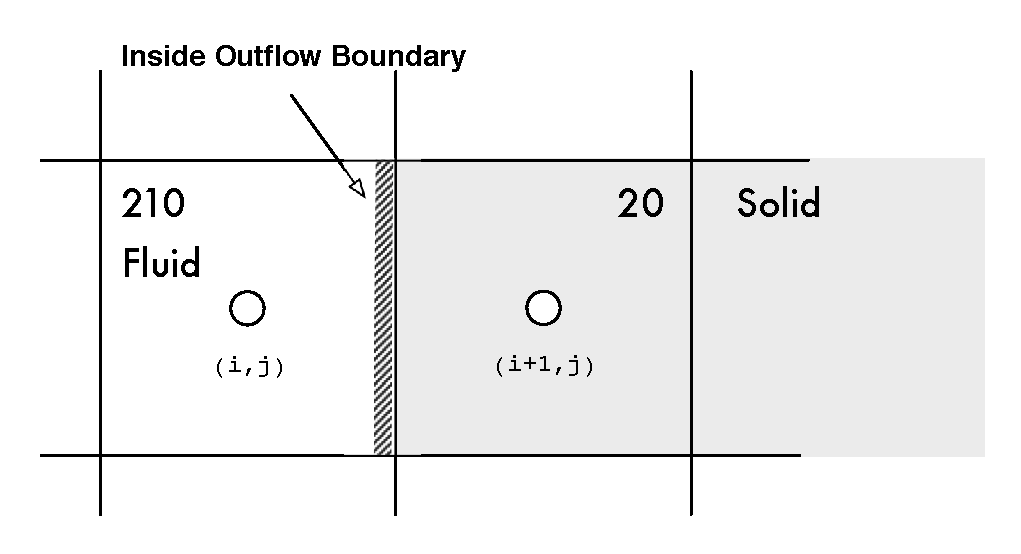
\includegraphics[width=9cm,clip]{outflowBC_inner.eps}
\end{center}
\caption{流出境界の設定.流出面の下流セルは固体とする.}
\label{fig:outflow BC inner}
\end{figure}

\noindent 流出速度の選び方として,経験上,内部流の場合にはAverageが流出速度のよい近似値を与える.
圧力境界として圧力勾配ゼロを指定している.

内部境界の流出fluxの計算は,現時点で一次風上となっているので,抜けにくい傾向があるかもしれない.


さて,Fractional Step法では,予測した疑似速度の発散に対して,連続の式を満足するように圧力場が収束していく.
そこで,Poisson方程式のソース項$\partial u_{\,i}^{\,*}/\partial x_{\,i}$に対して,次式のように流出境界面の指定速度が反映されるように修正している\footnote{SetBC3D::mod\_Psrc\_VBC(), cbc\_div\_ibc\_()を参照.}.

流出界面の流出速度には,次式の対流流出条件から時間進行した疑似速度ベクトルを用いる\footnote{SetBC3D::mod\_Pvec\_CF(), cbc\_vibc\_outflow\_cf\_()}.

\begin{equation}
{\frac{\partial u_{\,i}}{\partial t}}^{\,*} \,+\, {\left( u_{\,1} \right)}_{\,i+1/2} {\frac{\partial u_{\,i}}{\partial x}}^{\,n} \,=\, 0
\label{eq:outflow_cv}
\end{equation}


n+1ステップの速度を計算した後,流出セルフェイス面の速度を修正する.この修正されたセルフェイス速度を用いて,$div\,(\bm{u})^{\,n+1}$が評価され,収束判定に用いられる\footnote{収束判定のノルムの種類に$div\,(\boldmath $u$)^{\,n+1}$が指定されている場合.SetBC3D::modifyCFVelocity()を参照.}.

\begin{equation}
{\frac{\partial u_{\,i}}{\partial x_{\,i}}}^{\,*} \,=\, u_{\,i+1/2}^{\,n}-u_{\,i-1/2}^{\,*} + v_{\,j+1/2}^{\,*} - v_{\,j-1/2}^{\,*} + w_{\,k+1/2}^{\,*} - w_{\,k-1/2}^{\,*}
\label{eq:outflow modify poisson src}
\end{equation}

上記のように連続の式から逆に流出境界面速度を求める.しかしながらこの方法では,1つのセルに2つ以上の流出面は設定できない制限が生じる点に注意する.

%圧力の境界条件については,流出面で$\nabla p=0$を与える場合と,Dirichlet型$p=0$で与える場合を選択する.

\end{indentation}

\pagebreak
%
\hypertarget{tgt:inflow}{\subsubsection{速度指定境界}}
\label{sec:BC inflow}

速度指定境界は,流入境界として利用される.

\begin{indentation}{3zw}{0zw}

\paragraph{外部境界面}
流入境界を外部境界面に与える例を示す.

{ \small
\begin{program}
<OuterBoundary>
  <Elem id="2" name="Specified_Velocity">
    <Param dtype="REAL"   name="Normal_X"        value="1.0"/>
    <Param dtype="REAL"   name="Normal_Y"        value="0.0"/>
    <Param dtype="REAL"   name="Normal_Z"        value="0.0"/>
    <Param dtype="STRING" name="Specified_Type"  value="Velocity"/>
    <Param dtype="STRING" name="Profile"         value="Constant"/>
    <Param dtype="REAL"   name="Specified_Value" value="5.0"/>
  </Elem>
</OuterBoundary>
\end{program}
}

\textbf{図\ref{fig:inflow BC}}において,$w=i-1/2$面に速度$u_{\,1,\,\mathrm{in}}$を指定する場合を考える.セル$(i,\,j,\,k)$に対する流入条件なので$w$面の指定速度は$u_{\,1,\,\mathrm{in}}>0$になる.

\begin{equation}
{\left(\, \tilde{f}_i \,\right)}_{\,i-1/2,\,j,\,k} \,=\, u_{\,1,\,\mathrm{in}} \,\varphi_{\,\mathrm{in}}
\label{eq:inflow flux}
\end{equation}

\noindent 速度の流入境界の場合$\varphi$は次式となる.

\begin{equation}
\varphi_{\,\mathrm{in}} \,=\, u_{\,i,\,\mathrm{in}} \,+\,u_{\,i}^{\,g}
\label{eq:inflow flux}
\end{equation}

\begin{figure}[htbp]
\begin{center}
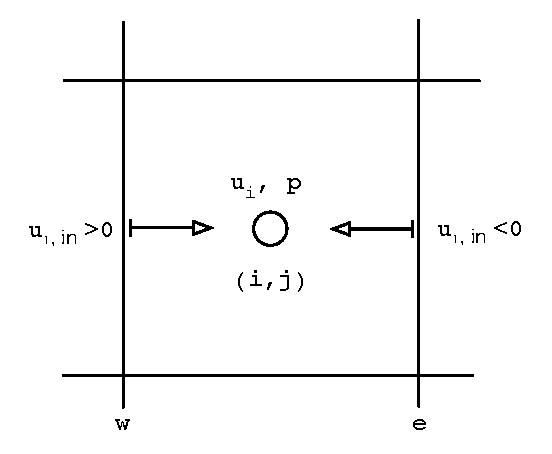
\includegraphics[width=5.5cm,clip]{inflowBC.eps}
\end{center}
\caption{速度指定境界.セル$\mathrm{(i,j)}$は流体セル,流入上流側の$\mathrm{(i\pm1,j)}$セルはガイドセル上で流体を指定する.}
\label{fig:inflow BC}
\end{figure}

速度指定境界条件は,流出条件と同様に流束型の境界条件として実装している\footnote{SetBC3D::mod\_Pvec\_Flux(), cbc\_pvec\_vobc\_()}.
指定部分で与えられた速度を用いて界面の流束を計算する.このとき,一次風上を用いているので,若干振動が残る.

圧力Poissonを解く場合の疑似速度の発散の修正は\verb|SetBC3D::mod_Psrc_VBC(), cbc_div_obc_vspec_()|で処理される.
また,セルフェイス速度は\verb|SetBC3D::mod\_Vec\_CF(), cbc\_vobc\_drchlt\_cf\_()|で計算する.

圧力の境界条件は,壁面境界条件と同様に,\textbf{式(\ref{eq:prs BC from NS})}のNavier-Stokes方程式からNeumann型の圧力境界条件が得られる.
流入境界における指定速度を$u_{\,i,\,in}$とすると,

\begin{equation}
{\left( \frac{\partial p}{\partial x_{\,i}}\right)}^{\,n+1}_{\,in} \,=\, - {\left( \frac{\partial u_{\,i}}{\partial t}\right)}^{\,n+1}_{\,in}
\,-\, \left( u_{\,j,\,in}-u_{\,j}^{\,g} \right) {\left( \frac{\partial u_{\,i}}{\partial x_{\,j}}\right)}_{\,in}
\,+\, \frac{1}{Re} {\left( \frac{\partial^{\,2} u_{\,i}}{\partial x_{\,j}^{\,2}} \right)}_{\,in}
\label{eq:prs inflow BC from NS}
\end{equation}

\noindent 高レイノルズ数流れにおいては,粘性項の寄与が小さいと仮定し粘性項を省略している.



\paragraph{内部領域}

指定方法として,Dirichlet型の速度境界条件を用いて,セルフェイス位置の運動量流束を直接与える.計算内部領域における流入境界のXML入力パラメータは下記のように指定する.

{\small
\begin{program}
<InnerBoundary> 
  <Elem name="specified_velocity" id="3" comment="inlet">
    <Param name="Normal_x"        dtype="REAL"   value="0.0" />
    <Param name="Normal_y"        dtype="REAL"   value="0.0" />
    <Param name="Normal_z"        dtype="REAL"   value="-1.0" />
    <Param name="def_face"        dtype="INT"    value="6" />
    <param name="Profile"         dtype="string" value="Harmonic" />
    <param name="Specified_Type"  dtype="string" value="Velocity" />
    <Param name="Specified_Value" dtype="REAL"   value="7.0" />
    <Param name="Frequency"       dtype="REAL"   value="2.0" />
    <Param name="Initial_Phase"   dtype="REAL"   value="0.0" />
    <Param name="Constant_Bias"   dtype="REAL"   value="0.0" />
    <Param name="Temperature"     dtype="REAL"   value="50.0" />
  </Elem>
</InnerBoundary>
\end{program}
}

\noindent 境界面の指定方法は流出境界と同様である.つまり,流入の上流側のセルには固体属性を与える.前述のXMLの指定の例では,id=6は流体セル,id=3は固体セルとなる.
ベクトルの指定は,法線成分とベクトルの大きさで与える.
時間的に変化しない場合にはtype=constantを指定する.
時間変化を伴う速度指定はtype=Harmonicを指定し,\textbf{式(\ref{eq:harmonic_v})}の形式の単振動\index{たんしんどう@単振動}の境界条件を周期や初期位相,切片(初期振幅)とともに与える.非定常の場合,振幅はvelocityで与えられる.
各パラメータは\textbf{表\ref{tbl:harmonic_table_v_obc}}に対応する.

\end{indentation}


\pagebreak
%
\subsubsection{周期境界}
\label{sec:BC periodic}

周期境界条件には,外部領域面に対する周期境界と計算内部領域に設定する部分的な周期境界条件を併用する条件の2種類を想定.

\begin{indentation}{3zw}{0zw}

\paragraph{外部領域面}

外部領域面に対する周期境界条件では,\textbf{図\ref{fig:index_domain}}において,Inner\,Regionの両端の境界が重なる状態を想定している.
外部領域面に対する周期境界条件には\textbf{表\ref{tbl:periodic mode}}に示す3つのモードが指定できる.

\begin{table}[htdp]
\caption{周期境界条件のモード}
\begin{center}
\small
\begin{tabular}{ll} \toprule
キーワード & モードの説明\\ \midrule
Simple\_Copy & 周期境界の両端で物理量をガイドセルにコピー.\\
Directional  & 圧力差を与える周期境界条件で,上流と下流の境界面を指定.\\
Driver       & 計算領域内で部分的な周期境界条件を設定.\\ \bottomrule
\end{tabular}
\end{center}
\label{tbl:periodic mode}
\end{table}

\begin{enumerate}
\item Simple\_Copyモード\\
周期境界条件面の両端で,単純に計算内部領域の値を他方のガイドセルにコピー.
\item Directionalモード\\
両端で圧力差を与える周期境界条件で,速度や温度についてはSimple\_Copyモードと同じだが,圧力は指定の圧力差を与える.上流側と下流側の設定が必要.
\item Driverモード\\
乱流計算などで発達したチャネル流を上流境界として与えるためのしくみで,内部境界条件との組み合わせで利用.Driverモードの説明は内部境界条件を参照.
\end{enumerate}


{\small
\begin{program}
<OuterBoundary>
  <Elem name="Basic_BCs">
    <Elem name="periodic" id="7" >
      <Param name="mode" dtype="string" value="Simple_Copy" />
    </Elem>
      
    <Elem name="periodic" id="8" >
      <Param name="mode"                dtype="string" value="Directional" />
      <Param name="flow_direction"      dtype="string" value="upstream" />
      <Param name="pressure_difference" dtype="REAL"   value="8.148e-3" />
    </Elem>
      
    <Elem name="periodic" id="9" >
      <Param name="mode"                dtype="string" value="Directional" />
      <Param name="flow_direction"      dtype="string" value="downstream" />
      <Param name="pressure_difference" dtype="REAL"   value="8.148e-3" />
    </Elem>
      
    <Elem name="periodic" id="10" >
      <Param name="mode"             dtype="string" value="driver" />
      <Param name="driver_direction" dtype="string" value="x_minus" />
    </Elem>
  </Elem>
</OuterBoundary>
\end{program}
}


Directionalモードでは,\textbf{表\ref{tbl:parameter dir. mode}}に示すパラメータが必要で,Pressure\_Differenceの値が,UpstreamとDownstreamで同じ値である必要がある.

\begin{table}[htdp]
\caption{Directionalモードに必要なパラメータ}
\begin{center}
\small
\begin{tabular}{ll} \toprule
必要なキーワード & パラメータの説明\\ \midrule
Pressure\_Difference & 両端にかける圧力差 $[Pa]$\\
Flow\_Direction & Upstream(上流面)または Downstream(下流面)\\
\bottomrule
\end{tabular}
\end{center}
\label{tbl:parameter dir. mode}
\end{table}


物理変数$\varphi$に対する周期境界条件は,Collocated変数配置\index{へんすうはいち@変数配置!コロケート@Collocated---}において,各方向について次式のように設定される.
適用の制限として,周期境界上には物体と他の境界条件を設定しないこと.

\begin{equation}
\begin{array}{ccc}
\left\{ \,\, \begin{array}{lll}
\varphi_{\,-2,\,j,\,k}   &=& \varphi_{\,ix-2,\,j,\,k}\\
\varphi_{\,-1,\,j,\,k}   &=& \varphi_{\,ix-1,\,j,\,k}\\
\varphi_{\,0,\,j,\,k}    &=& \varphi_{\,ix,\,j,\,k}\\
\varphi_{\,ix+1,\,j,\,k} &=& \varphi_{\,1,\,j,\,k}\\
\varphi_{\,ix+2,\,j,\,k} &=& \varphi_{\,2,\,j,\,k}
\end{array} \right. \quad
&
\left\{ \,\, \begin{array}{lll}
\varphi_{\,i,-2,\,k}     &=& \varphi_{\,i,\,jx-2,\,k}\\
\varphi_{\,i,-1,\,k}     &=& \varphi_{\,i,\,jx-1,\,k}\\
\varphi_{\,i,0,\,k}      &=& \varphi_{\,i,\,jx,\,k}\\
\varphi_{\,i,\,jx+1,\,k} &=& \varphi_{\,i,\,1,\,k}\\
\varphi_{\,i,\,jx+2,\,k} &=& \varphi_{\,i,\,2,\,k}
\end{array} \right. \quad
&
\left\{ \,\, \begin{array}{lll}
\varphi_{\,i,\,j,\,-2}   &=& \varphi_{\,i,\,j,\,kx-2}\\
\varphi_{\,i,\,j,\,-1}   &=& \varphi_{\,i,\,j,\,kx-1}\\
\varphi_{\,i,\,j,\,0}    &=& \varphi_{\,i,\,j,\,kx}\\
\varphi_{\,i,\,j,\,kx+1} &=& \varphi_{\,i,\,j,\,1}\\
\varphi_{\,i,\,j,\,kx+2} &=& \varphi_{\,i,\,j,\,2}
\end{array} \right.
\end{array}
\label{eq:periodic BC}
\end{equation}


\end{indentation}


\pagebreak
%
\subsubsection{遠方境界}
\label{sec:BC trc_free}

\begin{indentation}{3zw}{0zw}
トラクションフリー条件は,外部境界に対してのみ指定できる.
この境界条件は,計算対象の主領域から遠方の挙動を仮定した条件で,計算外部境界において流体の内部応力の法線方向成分がゼロである仮定を用いる.
この境界条件は,噴流のエントレインメントの効果などを考慮できる利点があるが,渦が流出するような境界には適用できない.
内部応力テンソルを$T_{\,ij}$, 計算外部境界の外向き法線を$n_{\,j}$とすると,

\begin{equation}
T_{\,ij} \,=\, - p \,\delta_{\,ij} \,+\,\nu \left( \frac{\partial u_{\,i}}{\partial x_{\,j}} \,+\, \frac{\partial u_{\,j}}{\partial x_{\,i}} \right)
\label{eq:Traction}
\end{equation}

\begin{equation}
T_{\,ij}\, n_{\,j} \,=\, 0
\label{eq:Tfree}
\end{equation}

\noindent 例えば,X軸の正負方向のトラクション成分を表す式は,次のように導出される.

\begin{equation}
\left[
\begin{array}{ccc}
T_{\,11} & T_{\,12} & T_{\,13}\\
T_{\,21} & T_{\,22} & T_{\,23}\\
T_{\,31} & T_{\,32} & T_{\,33}\\
\end{array} \right] \left[
\begin{array}{c}
\pm1\\
0\\
0\\
\end{array}
\right]
\,=\,
\pm \left[ 
\begin{array}{c}
T_{\,11}\\
T_{\,21}\\
T_{\,31}\\
\end{array} \right]
\,=\, \pm T_{\,i1} \,=\, 0
\label{eq:trc_eq}
\end{equation}

\noindent したがって,各外部境界面に対する解くべき式は次のように表せる.

\begin{equation}
\left .
\begin{array}{lll}
x & ; & T_{\,i1}\,=\,0 \\
y & ; & T_{\,i2}\,=\,0 \\
z & ; & T_{\,i3}\,=\,0  
\end{array}
\right \}
\label{eq:trc_eq2}
\end{equation}

\noindent 例えば,これからx方向の式を導くと,\textbf{式(\ref{eq:trc_eq3})}のようになる.

\begin{equation}
\left .
\begin{array}{l}
\vspace{2mm}
\displaystyle{ T_{\,11} \,=\, -p \,+\, 2 \nu \frac{\partial u_{\,1}}{\partial x_{\,1}} }\\
\vspace{2mm}
\displaystyle{ T_{\,21} \,=\, \frac{\partial u_{\,2}}{\partial x_{\,1}} + \frac{\partial u_{\,1}}{\partial x_{\,2}} }\\
\vspace{2mm}
\displaystyle{ T_{\,31} \,=\, \frac{\partial u_{\,3}}{\partial x_{\,1}} + \frac{\partial u_{\,1}}{\partial x_{\,3}} } 
\end{array}
\right \}
\label{eq:trc_eq3}
\end{equation}

\noindent \textbf{図\ref{fig:x-trc}}では,速度成分を$u,\,v,\,w$で表し,添え字で格子インデクスを表している.各方向の式を\textbf{式(\ref{eq:trc_cnd})}に示す.

\begin{figure}[htbp]
\begin{center}
\subfigure[X-方向のインデクス.]{
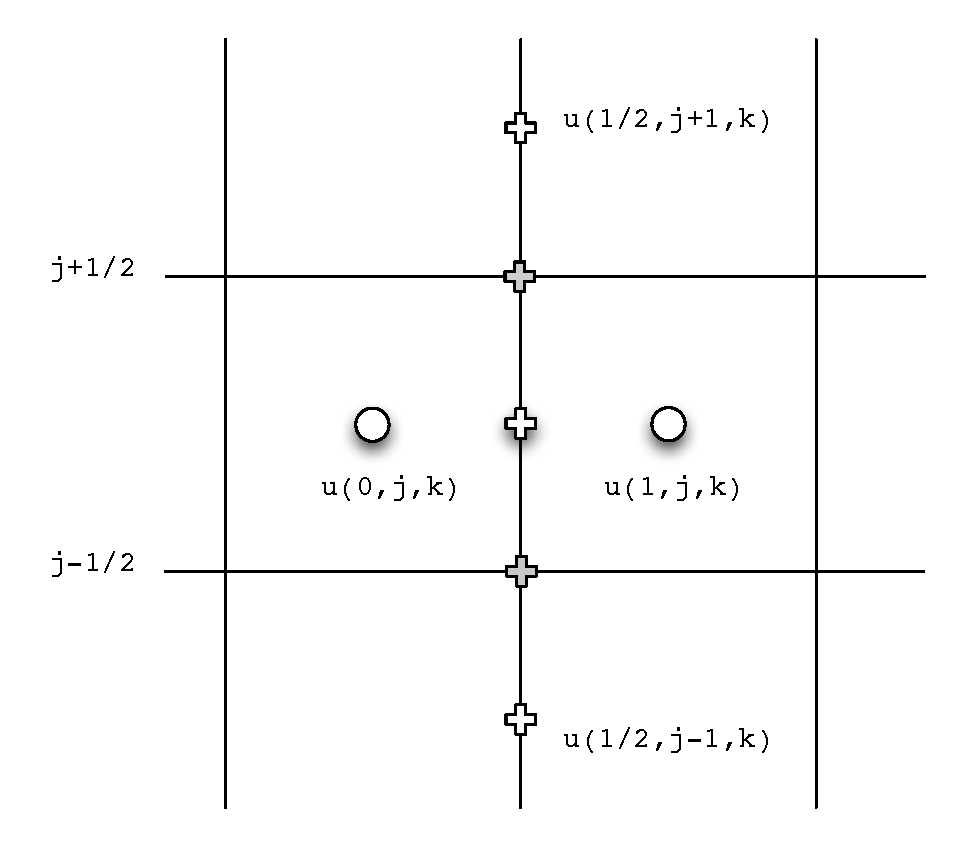
\includegraphics[height=6cm,clip]{T11.eps}
}~
\subfigure[X+方向のインデクス.]{
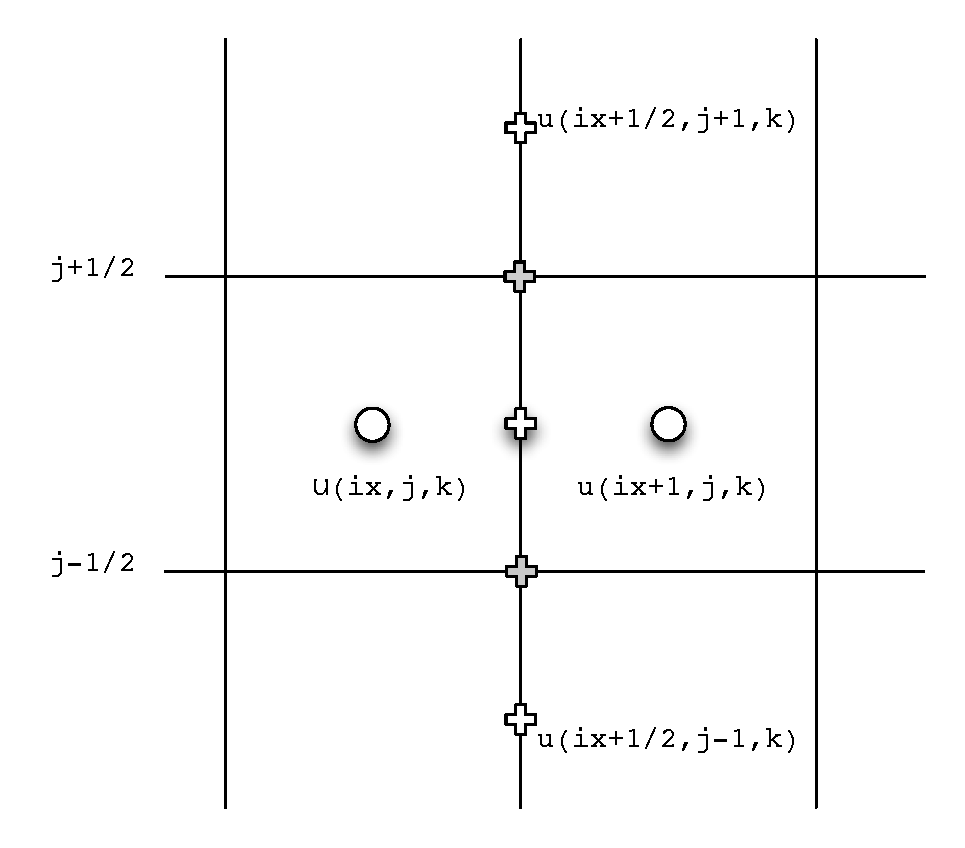
\includegraphics[height=6cm,clip]{T11+.eps}
}
\caption{外部境界のインデクス.○はセルセンターの定義点,十字(白)はスタガード位置の定義点,十字(灰)は外部境界面上の差分近似点で,定義点の値を用いて置き換える.} 
\label{fig:x-trc}
\end{center}
\end{figure}

\noindent 格子幅を$h$として$T_{\,21}$を外部境界面上で評価すると,
\begin{equation}
\left.
\begin{array}{l}
\vspace{1mm}
\displaystyle{ \frac{v_{\,1,\,j,\,k}-v_{\,0,\,j,\,k}}{h} \,+\, \frac{u_{\,1/2,\,j+1/2,\,k}-u_{\,1/2,\,j-1/2,\,k}}{h} \,\approx\, 
\frac{v_{\,1,\,j,\,k}-v_{\,0,\,j,\,k}}{h} \,+\, \frac{1}{2} \frac{u_{\,1/2,\,j+1,\,k}-u_{\,1/2,\,j-1,\,k}}{h} \,=\, 0 }\\
\vspace{1mm}
\displaystyle{ v_{\,0,\,j,\,k} \,=\, v_{\,1,\,j,\,k} \,+\, \frac{1}{2} \left( u_{\,1/2,\,j+1,\,k}-u_{\,1/2,\,j-1,\,k} \right) }\\
\end{array} \,\, \right\}
\label{eq:trc_T21}
\end{equation}

\noindent $u$はセルセンタ位置にあり,固体セルによる影響をマスク関数$\phi$で表すと,
\begin{equation}
\phi_{1/2,\,j,\,k} \,=\, \phi_{0,\,j,\,k} \times \phi_{1,\,j,\,k} \,=\,
\left\{
\begin{array}{ll}
0 & solid\\
1 & fluid\\
\end{array}
\right.
\end{equation}

\begin{equation}
u_{1/2,\,j\pm1,\,k} \,=\,(2u_{ref}-u_j)(1-\phi) + u_{j\pm1}\phi
\end{equation}

同様に,$T_{\,31}$から,
\begin{equation}
w_{\,0,\,j,\,k} \,=\, w_{\,1,\,j,\,k} \,+\, \frac{1}{2} \left( u_{\,1/2,\,j,\,k+1}-u_{\,1/2,\,j,\,k-1} \right)
\label{eq:trc_T31}
\end{equation}

\noindent $T_{\,11}$は圧力の遠方条件$p=0$(基準圧)を考慮して,
\begin{equation}
\frac{\partial u}{\partial x} \,=\, 0 \quad \mapsto \quad u_{\,0,\,j,\,k} \,=\, u_{\,1,\,j,\,k}
\label{eq:trc_T11}
\end{equation}

したがって,各方向の境界条件の式は以下のようになる.

\begin{equation}
\left.
\begin{array}{llll}
\vspace{1mm}
x-; & u_{\,0,\,j,\,k} &=& u_{\,1,\,j,\,k} \\
\vspace{1mm}
& v_{\,0,\,j,\,k} &=& \displaystyle{ v_{\,1,\,j,\,k} \,+\, \frac{1}{2}\left( \tilde{u}_{\,1/2,\,j+1,\,k}-\tilde{u}_{\,1/2,\,j-1,\,k}\right)}\\
\vspace{3mm}
& w_{\,0,\,j,\,k} &=& \displaystyle{ w_{\,1,\,j,\,k} \,+\, \frac{1}{2}\left( \tilde{u}_{\,1/2,\,j,\,k+1}-\tilde{u}_{\,1/2,\,j,\,k-1}\right)}\\

\vspace{1mm}
x+; & u_{\,ix+1,\,j,\,k} &=& u_{\,ix,\,j,\,k} \\
\vspace{1mm}
& v_{\,ix+1,\,j,\,k} &=& \displaystyle{ v_{\,ix,\,j,\,k} \,-\, \frac{1}{2}\left( \tilde{u}_{\,ix+1/2,\,j+1,\,k}-\tilde{u}_{\,ix+1/2,\,j-1,\,k}\right)}\\
\vspace{3mm}
& w_{\,ix+1,\,j,\,k} &=& \displaystyle{ w_{\,ix,\,j,\,k} \,-\, \frac{1}{2}\left( \tilde{u}_{\,ix+1/2,\,j,\,k+1}-\tilde{u}_{\,ix+1/2,\,j,\,k-1}\right)}\\

\vspace{1mm}
y-; & u_{\,i,\,0,\,k} &=& \displaystyle{ u_{\,i,\,1,\,k} \,+\, \frac{1}{2}\left( \tilde{v}_{\,i+1,\,1/2,\,k}-\tilde{v}_{\,i-1,\,1/2,\,k}\right)}\\
\vspace{1mm}
& v_{\,i,\,0,\,k} &=& v_{\,i,\,1,\,k}\\
\vspace{3mm}
& w_{\,i,\,0,\,k} &=& \displaystyle{ w_{\,i,\,1,\,k} \,+\, \frac{1}{2}\left( \tilde{v}_{\,i,\,1/2,\,k+1}-\tilde{v}_{\,i,\,1/2,\,k-1}\right)}\\

\vspace{1mm}
y+; & u_{\,i,\,jx+1,\,k} &=& \displaystyle{ u_{\,i,\,jx,\,k} \,-\, \frac{1}{2}\left( \tilde{v}_{\,i+1,\,jx+1/2,\,k}-\tilde{v}_{\,i-1,\,jx+1/2,\,k}\right)}\\
\vspace{1mm}
& v_{\,i,\,jx+1,\,k} &=& v_{\,i,\,jx,\,k}\\
\vspace{4mm}
& w_{\,i,\,jx+1,\,k} &=& \displaystyle{ w_{\,i,\,jx,\,k} \,-\, \frac{1}{2}\left( \tilde{v}_{\,i,\,jx+1/2,\,k+1}-\tilde{v}_{\,i,\,jx+1/2,\,k-1}\right)}\\

\vspace{1mm}
z-; & u_{\,i,\,j,\,0} &=& \displaystyle{ u_{\,i,\,j,\,1} \,+\, \frac{1}{2}\left( \tilde{w}_{\,i+1,\,j,\,1/2}-\tilde{w}_{\,i-1,\,j,\,1/2}\right)}\\
\vspace{1mm}
& v_{\,i,\,j,\,0} &=& \displaystyle{ v_{\,i,\,j,\,1} \,+\, \frac{1}{2}\left( \tilde{w}_{\,i,\,j+1,\,1/2}-\tilde{w}_{\,i,\,j-1,\,1/2}\right)}\\
\vspace{3mm}
& w_{\,i,\,j,\,0} &=& w_{\,i,\,j,\,1}\\

\vspace{1mm}
z-; & u_{\,i,\,j,\,kx+1} &=& \displaystyle{ u_{\,i,\,j,\,kx} \,-\, \frac{1}{2}\left( \tilde{w}_{\,i+1,\,j,\,kx+1/2}-\tilde{w}_{\,i-1,\,j,\,kx+1/2}\right)}\\
\vspace{1mm}
& v_{\,i,\,j,\,kx+1} &=& \displaystyle{ v_{\,i,\,j,\,kx} \,-\, \frac{1}{2}\left( \tilde{w}_{\,i,\,j+1,\,kx+1/2}-\tilde{w}_{\,i,\,j-1,\,kx+1/2}\right)}\\
\vspace{3mm}
& w_{\,i,\,j,\,kx+1} &=& w_{\,i,\,j,\,kx}
\end{array} \qquad \right \}
\label{eq:trc_cnd}
\end{equation}

実装では,外部境界上にある壁面の速度成分も考慮している.

j=jxの場合に,$u_{0,\,jx+1,\,k}$の値を参照するので,境界条件処理で値を代入しておく必要がある.

次の例では,遠方圧力に$p=0$[Pa\_g]\footnote{ゲージ圧,Steer $>$ Unit $>$ PressureでGaugeを指定しておく.}を指定した境界条件ID=4に遠方境界条件を設定する.熱流れの場合には,遠方場における温度を指定.
{ \small
\begin{program}
<OuterBoundary>
  <Elem name="Basic_BCs">
    <Elem name="traction_free" id="4">
      <Param name="Ambient_Temperature" dtype="REAL" value="25.0" />
    </Elem>
  </Elem>
</OuterBoundary>
\end{program}
}
\end{indentation}


\pagebreak
%
\subsubsection{流入出境界}
\label{sec:BC in_out}

\begin{indentation}{3zw}{0zw}
振動流のための特殊な境界条件である.指定された外部境界面において,境界流速の符号に応じて流出と遠方条件を切り替える.
境界流速には境界面の平均流速を用いる.

下記の例では,流出境界条件に切り替わった場合の対流流出速度のパラメータをMinmaxに指定.

{\small
\begin{program}
<OuterBoundary>
  <Elem name="in_out" id="5">
    <Param name="velocity_type" dtype="STRING" value="minmax" />
    <Param name="Ambient_Temperature" dtype="REAL" value="25.0" />
  </Elem>
</OuterBoundary>
\end{program}
}

熱流れの場合には,流入時に対応する温度を指定.

\end{indentation}

\pagebreak
%
\subsection{静止座標系と移動座標系の場合の境界条件}
\label{sec:moving_grid}
外部流を考える.
\textbf{図\ref{fig:reference_frame}}(a)の静止座標系\index{ざひょうけい@座標系!せいし@静止---}と{図\ref{fig:reference_frame}}(b)の移動座標系\index{ざひょうけい@座標系!いどう@移動---}のように異なる座標系で物体まわりの流れを計算する場合,境界条件の与え方が異なる.
静止座標系は風洞実験に相当し,静止した対象物に対して風をあてる.テストセクション(この場合は計算領域)から出ていく流れが流出風に相当する.
一方,移動座標系では対象物に固定した計算格子が対象物とともに静止流体中を移動する.この場合は,計算領域そのものと内部の格子が物体とともに動く.
一定速度$V$で動いている座標系の添え字を${}_M$とし,静止した座標系の添え字を${}_S$とする.
いま,静止座標系で観測される流体の速度を$u_{S}$と表すと,同じ速度は移動座標系では$u_{M}-V$のように観測される.
つまり,
\begin{equation}
u_{S} \, = \, u_{M}-V
\label{eq:galilei}
\end{equation}
両者は\textbf{式(\ref{eq:galilei})}のガリレイ変換\index{がりれいへんかん@ガリレイ変換}に対して不変である.

\begin{figure}[htbp]
\begin{center}
\subfigure[静止座標系]{
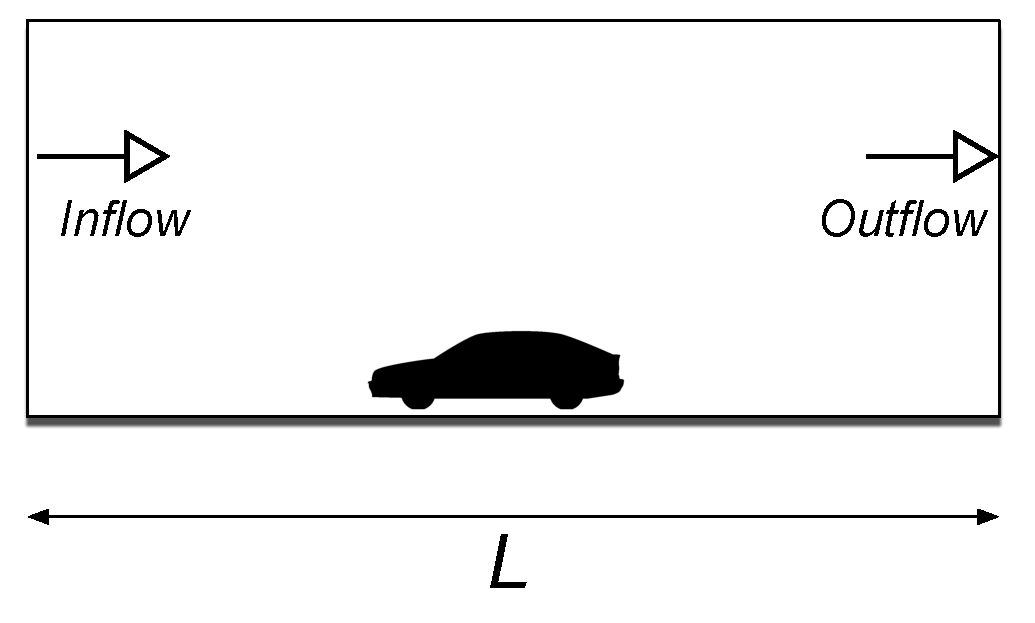
\includegraphics[width=8cm,clip]{stationary.eps}
}
~
\subfigure[移動座標系]{
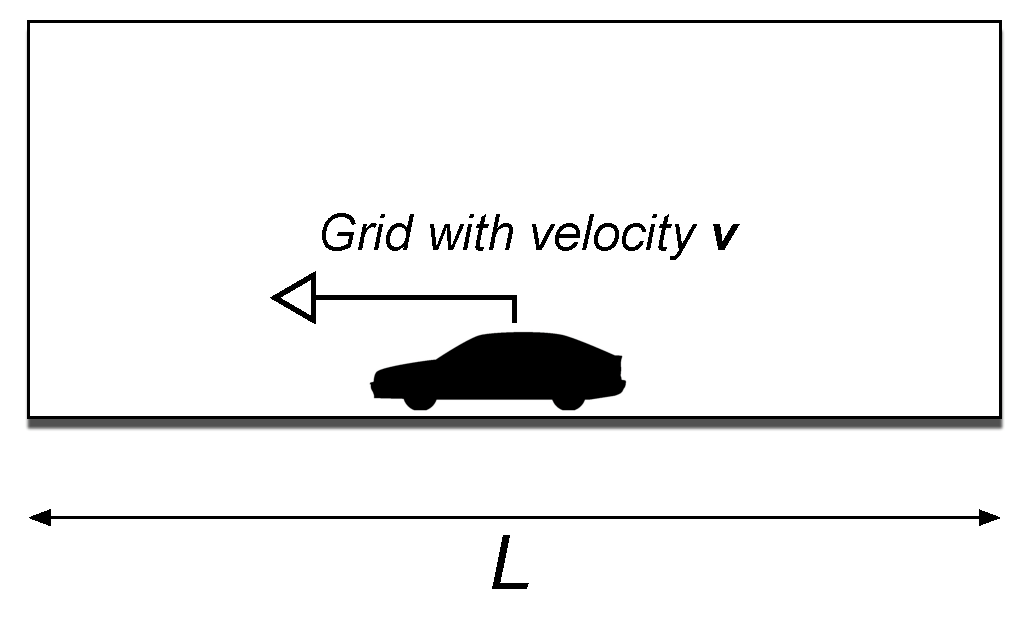
\includegraphics[width=8cm,clip]{moving.eps}
}
\caption{静止座標系と移動座標系の観測点の違い} 
\label{fig:reference_frame}
\end{center}
\end{figure}

静止座標系において\textbf{図\ref{fig:reference_frame}}(a)のような境界条件を与える場合,流入部では$u_{0}$を与える.
一方,移動座標系では静止流体の条件,つまり$u=0,\,p=0$を想定し,格子速度$V=-u_{0}$を与えると両者は等価になる.

移動座標系の場合注意を要するのが,物体と地面の境界条件である.物体は移動しているので格子速度と同じである.
一方,地面は静止している地面と動いている地面の二通りが考えられる.
前者は風洞実験で固定地面板に相当し,後者はムービングベルトに相当する.
ムービングベルトの場合には物体と格子速度だけ相対速度をもっている.
したがって,

\begin{equation}
u_{ground}\,=\,
\begin{cases}
\, -u_{0} & \quad (Stationary\,ground)\\
\, 0 & \quad (Moving\,ground)\\
\end{cases}
\label{eq:relative velocity wall}
\end{equation}

移動格子の移動速度はReference\_Frameセクションで与える.




%%%%%
\begin{comment}
%
%
\paragraph{Direct\_Forcing}
\begin{indentation}{3zw}{0zw}
%Direct\_Forcingによる指定は,速度定義点により記述するカテゴリが異なる.
Immersed Boundary Methodの定式化に従い,定義点において速度を強制する.
次の例では,ID=2のセルのスタガード位置の速度定義点に指定した法線と大きさをもつ速度を強制する.
モニター量はない.

{ \small
\begin{program}
<Elem name="Vec_Face" id="1">
  <Elem name="direct_forcing" id="2" comment="f1">
    <Param name="Norm_x"      dtype="REAL"   value="1.0" />
    <Param name="Norm_y"      dtype="REAL"   value="0.0" />
    <Param name="Norm_z"      dtype="REAL"   value="0.5" />
    <Param name="velocity"    dtype="REAL"   value="0.5" />
  </Elem>
</Elem>
\end{program}
}

%%%

次の例は,セルセンタ位置での指定を示す.
{ \small
\begin{program}
<Elem name="Vec_Center" id="1">
  <Elem name="direct_forcing" id="2" comment="f1">
    <Param name="Norm_x"      dtype="REAL"   value="1.0" />
    <Param name="Norm_y"      dtype="REAL"   value="0.0" />
    <Param name="Norm_z"      dtype="REAL"   value="0.5" />
    <Param name="velocity"    dtype="REAL"   value="0.5" />
  </Elem>
</Elem>
\end{program}
}

%%%
\end{indentation}

\end{comment}
%%%%%


\pagebreak
%
\subsection{外力項を用いた境界条件}

\subsubsection{圧力損失・利得を伴う境界条件}
熱交換器やファンなどの圧力損失\index{あつりょくそんしつ@圧力損失}・利得をモデル化した境界条件について説明する.
熱交換器は,圧力損失を生じる多孔質物体で,流出方向が法線で与えられる.圧力損失は通過流量(流速)と圧力損失量の関係式が与えられるものとする.
一方,ファンは流量と圧力利得が関係式として与えられる.ファンの場合には旋回成分などもあるが,ここでは軸流方向のみを考える.
このような流体部品のモデル指定は,セルボリュームに作用する内部境界条件として指定し,コンポーネントを用いて実装する.
具体的には,\textbf{式(\ref{eq:ploss_NS})}の外力項$F_{i}$として実装する.$\beta$はセル内部におけるコンポーネントの体積占有率\index{せんゆうりつ@占有率}(Volume Fraction; VF)\index{Volume Fraction}である.
外力項として,\textbf{表\ref{tbl:ploss_model}}のようなモデルが実装されている.

この境界条件に対応する指定部の平均速度・流量や圧力損失量がhistory\_compo.logにモニタ量として書き出される.

\begin{table}[htdp]
\caption{セルボリュームに作用する内部境界条件}
\begin{center}
\small
\begin{tabular}{lll} \toprule
XMLキーワード & 境界条件モデル & モニター量\\ \midrule
%Fan & ファンモデル & \\ 
Pressure\_Loss & 圧力損失モデル & 通過風速,圧力損失量\\ 
%Darcy & 多孔質体に対するDarcyモデル & \\ 
\bottomrule
\end{tabular}
\end{center}
\label{tbl:ploss_model}
\end{table}

\begin{equation}
{\frac{\partial{u}_{i}}{\partial{t}}}^{{n}{+}{1}}{+}\,\frac{\partial}{\partial{x}_{j}}\left({{u}_{i}{u}_{j}}\right)
\,{=}\,
{-}{\frac{\partial{p}}{\partial{x}_{i}}}^{{n}{+}{1}}{+}\,{(}{1}{-}\mathrm{\beta}{)}\frac{\partial{\mathrm{\tau}}_{ij}}{\partial{x}_{j}}\,{+}\,\beta {F_{i}}^{n+1}
\label{eq:ploss_NS}
\end{equation}

%
\paragraph{Pressure\_Loss}
\begin{indentation}{3zw}{0zw}
圧力損失モデルは,膜や熱交換器などのモデリングとして利用され,\textbf{式(\ref{eq:ploss_NS})}に\textbf{式(\ref{eq:ploss_force})}の実験式を適用する.
\begin{equation}
{F}_{i}
\,{=}\,
-sgn \left( u_{i} \right) {\left( \frac{\Delta p}{\Delta r} \right)}^{R} {n_{i}}^{R}
\label{eq:ploss_force}
\end{equation}

\noindent ここで,${}^{R}$は圧力損失部を表し,$\Delta p,\,\Delta r,\,n_{i}$はそれぞれ圧力損失量,圧力損失部の厚さ,法線方向を表す.圧力損失部の通過ベクトルとは逆方向に圧力損失が発生するモデルとなっている.ただし,\textbf{表\ref{tbl:ploss_table_ibc}}で指定するパラメータvectorがdirectionalでない場合には,速度ベクトルは圧力損失部の流出方向には揃わない.単に,圧力損失が計算された速度ベクトルと逆向きに作用するモデルとなる.

圧力損失パラメータは,圧力損失部の試験結果により,\textbf{図\ref{fig:ploss}}に示すような実験値が得られる.
$\Delta p-V$の性能線図を$[mmAq - m/s]$を単位とした場合のパラメータの取得について示す.
圧力損失部の圧力損失は大抵二次多項式で近似できる.
\textbf{図\ref{fig:ploss}}のグラフの読みからカーブフィットを行い,\textbf{式(\ref{eq:dp-v})}に対応する数値$c_{1}$ -- $c_{4}$, $u_{threshold}$を得る.ダッシュは有次元を表す.
このとき,圧力損失ヘッドの単位に応じて,パラメータは無次元量に変換している.

\begin{equation}
{h}^{\prime}
\,{=}\,
\begin{cases}
\, c_{1} {u^{\prime}}^{2}\,+\,c_{2}u^{\prime}\,+\,c_{3} & \quad (u^{\prime} \geqq u^{\prime}_{threshold})\\
\, c_{4} {u^{\prime}}^{2} & \quad (u^{\prime}<u^{\prime}_{threshold})\\
\end{cases} \quad [mm]
\label{eq:dp-v}
\end{equation}

\vspace{5mm}

\begin{figure}[htdp]
  \begin{minipage}{.47\textwidth}
    \begin{center}
  	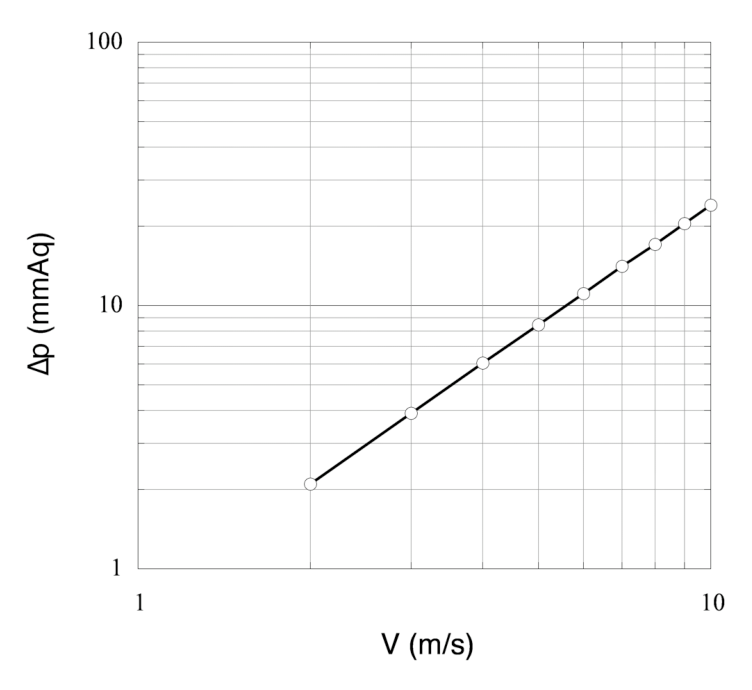
\includegraphics[width=6.5cm,clip]{ploss.eps}
  	\end{center}
  	\caption{$\Delta p-V$性能線図(対数表示)}
  	\label{fig:ploss}
  \end{minipage} \hfill
  \begin{minipage}{.47\textwidth}
    \begin{center}
    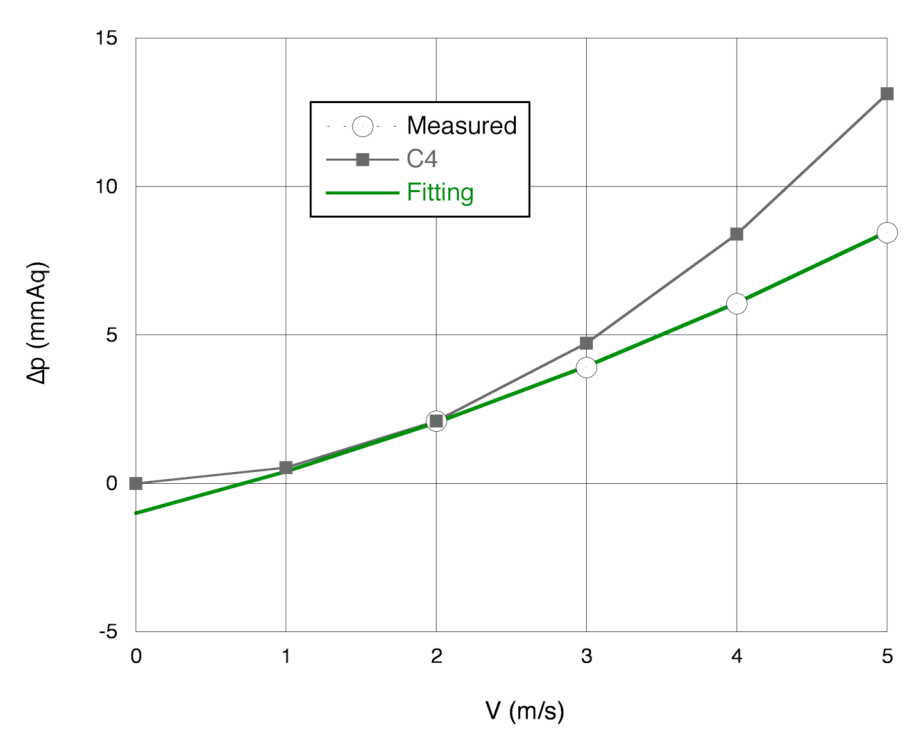
\includegraphics[width=7.5cm,clip]{rad_para.eps}
    \caption{パラメータの取得(\textbf{図\ref{fig:ploss}}と同じものを線形表示)}
    \label{fig:get_para}
    \end{center}
  \end{minipage}
\end{figure}

\textbf{図\ref{fig:get_para}}に計算パラメータの取得方法を示す.一般に,低速域のデータは得られない場合が多い.図では,○が測定結果を示し2$[m/s]$より低速域のデータはない.そこで,測定値を元にカーブフィッティングを行い(図中の緑色の曲線),算出された係数$c_{1}=0.12321,\,c_{2}=1.2806,\,c_{3}=-1.0074\quad(2-10\,[m/s])$を計算パラメータとする.この場合,$h'$切片がマイナスになるため,熱交換機の通過速度がゼロに近い場合に急にマイナスの圧力損失(つまり圧力利得)が発生し,実際の現象とは異なり計算上好ましくない.そこで\textbf{式(\ref{eq:dp-v})}に示すようにある閾値で曲線を切り替える.ここでは,測定された最小速度$u_{threshold}=2\,[m/s]$を閾値として,図中のC4のカーブ$c_{4}=0.525\quad(0-2\,[m/s])$で切り替える.圧力損失部厚さは実務での観点から単位を$[mm]$で指定するので,注意のこと.詳細については,\ref{sec:external force method}を参照.

次の例では,境界条件番号50に圧力損失条件を設定する.
ここで各パラメータは\textbf{表\ref{tbl:ploss_table_ibc}}に対応する.
{ \small
\begin{program}
<Elem name="Pressure_Loss" id="50" comment="radiator">
  <Param name="Normal_x"    dtype="REAL"   value="5.0" />
  <Param name="Normal_y"    dtype="REAL"   value="0.0" />
  <Param name="Normal_z"    dtype="REAL"   value="-1.0" />
  <Param name="c1"          dtype="REAL"   value="2.0" />
  <Param name="c2"          dtype="REAL"   value="10.0" />
  <Param name="c3"          dtype="REAL"   value="0.0" />
  <Param name="c4"          dtype="REAL"   value="0.0" />
  <Param name="u_threshold" dtype="REAL"   value="0.5" />
  <Param name="thickness"   dtype="REAL"   value="0.05" />
  <Param name="unit"        dtype="STRING" value="mmAq" />
  <Param name="vector"      dtype="STRING" value="directional" />
<\Elem>
\end{program}
}

\begin{table}[htdp]
\caption{圧力損失モデルのパラメータ}
\begin{center}
\small
\begin{tabular}{lll} \toprule
XMLキーワード & パラメータの説明\\ \midrule
Normal\_x & 圧力損失部の法線ベクトルのx方向成分\quad 法線は単位ベクトル\\
Normal\_y & 圧力損失部の法線ベクトルのy方向成分\quad 法線は単位ベクトル\\
Normal\_z & 圧力損失部の法線ベクトルのz方向成分\quad 法線は単位ベクトル\\
c1 & 圧力損失部の圧力損失係数\,c1\quad $[mmAq\,|\,mmHg\,|\,Pa]$\\
c2 & 圧力損失部の圧力損失係数\,c2\quad $[mmAq\,|\,mmHg\,|\,Pa]$\\
c3 & 圧力損失部の圧力損失係数\,c3\quad $[mmAq\,|\,mmHg\,|\,Pa]$\\
c4 & 圧力損失部の圧力損失係数\,c4\quad $[mmAq\,|\,mmHg\,|\,Pa]$\\
u\_threshold & 圧力損失カーブの切り替え速度 $u_{threshold}$ $[m/s]$\\
thickness & 圧力損失部の厚さ\quad $[mm]$\\
unit & 圧力損失$\Delta p-V$線図のヘッドの単位\quad [$mmAq\,|\,mmHg\,|\,Pa\,|\,Non-Dimension]$ \footnotemark[7]\\
vector & 速度ベクトルの法線方向への強制\quad $[Directional \,|\, Non-Directional]$\\  \bottomrule
\end{tabular}
\end{center}
\label{tbl:ploss_table_ibc}
\end{table}
\footnotetext[7]{mmAqは水(300K, p=101.325kPa)996.62 $[kg/m^3]$,mmHgは水銀(300K)13538 $[kg/m^3]$をプログラム中でハードコード.}
\end{indentation}






%%%%
\begin{comment}
\paragraph{Fan}
\begin{indentation}{3zw}{0zw}
Fanモデル...
\end{indentation}

%
\paragraph{Darcy model}
\label{Darcy model param}
\begin{indentation}{3zw}{0zw}

\ref{sec:porous model}で説明したDarcyモデルでは,等方と非等方モデルが利用できる.透過率パラメータは,\textbf{表\ref{tbl:permeability parameter}}に示すように各主軸方向毎に与える.等方モデルの場合には,各方向のパラメータを同じ値にする.

{ \small
\begin{program}
<Elem name="Forcing_Volume" id="1">
  <Elem name="Darcy" id="50" comment="porous">
    <Param name="permeability_x"  dtype="REAL" value="2.0" />
    <Param name="permeability_y"  dtype="REAL" value="3.0" />
    <Param name="permeability_z"  dtype="REAL" value="4.0" />
  <\Elem>
<\Elem>
\end{program}
}

\begin{table}[htdp]
\caption{Darcyモデルのパラメータ}
\begin{center}
\small
\begin{tabular}{ll} \toprule
XMLキーワード & パラメータの説明\\ \midrule
permeability\_x & x方向の透過率 $[m^2]$\\
permeability\_y & y方向の透過率 $[m^2]$\\
permeability\_z & z方向の透過率 $[m^2]$\\ \bottomrule
\end{tabular}
\end{center}
\label{tbl:permeability parameter}
\end{table}

\end{indentation}

\end{comment}
%%%%

%
\section{熱解析の境界条件}
\label{sec:thermal_condition}
非圧縮性流体近似されたエネルギー式,つまりパッシブスカラー型の温度輸送方程式について,温度の境界条件を説明する.流れの境界条件と同様に,まず,外部境界条件を\ref{sec:heat_ext_bc}で説明し,その後内部境界条件を\ref{sec:heat_int_bc}で説明する.内部境界条件には熱交換機での利用を想定した放熱境界条件を含む.

%
\subsection{外部境界条件の指定}
\label{sec:heat_ext_bc}
熱の外部境界条件は,\ref{sec:heat_boundary}で詳しく述べているが,断熱条件はマスク\index{マスク}により温度勾配ゼロの条件が直接反復式中に取り込まれる.また,熱伝導条件は拡散項で表現され多媒質の場合に物性値依存で熱移動が計算される.これらの2つ以外の境界条件は明示的に指定する.

\textbf{表\ref{tbl:temperature_obc}}に示す熱の外部境界条件について例示する.熱の境界条件は,全て有次元でパラメータを与える.

%
\paragraph{Dirichlet}
\begin{indentation}{3zw}{0zw}
指定面のガイドセルに指定温度を与える.
次の例では,境界条件番号40として,20.0 [${}^\circ \mathrm{C}$ or K]のDirichlet境界条件を設定する.温度の単位はUnit\_Temperatureに従う.
{ \small
\begin{program}
<Param name="dirichlet" dtype="REAL" value="20.0" id="40"/>
\end{program}
}
\end{indentation}

%%%
\begin{comment}
\paragraph{HeatFlux}
\begin{indentation}{3zw}{0zw}
指定面に熱流束を指定する.
次の例では,境界条件番号40として,熱流束境界条件を設定する.
{ \small
\begin{program}
<Param name="HeatFlux" dtype="REAL" value="" id="40"/>
\end{program}
}
\end{indentation}
\end{comment}
%%%

%
\paragraph{Insulation}
\begin{indentation}{3zw}{0zw}
指定面で断熱条件を指定する.
断熱条件の実効的な実装は,内部境界条件の断熱指定によるので,ここでは単にガイドセルへの値のコピーを行っているだけである.
次の例では,境界条件番号30に断熱条件$\partial \theta / \partial x_i = 0$を指定する.
{ \small
\begin{program}
<Param name="Insulation" dtype="REAL" value="" id="30"/>
\end{program}
}
\end{indentation}

%%%
\begin{comment}
\paragraph{IsoThermal}
\begin{indentation}{3zw}{0zw}
指定面で一定温度を指定する.
次の例では,境界条件番号40として,20.0の等温境界条件を設定する.温度の単位はUnit\_Temperatureに従う.
{ \small
\begin{program}
<Param name="IsoThermal" dtype="REAL" value="20.0" id="40"/>
\end{program}
}
\end{indentation}
\end{comment}
%%%

%
\paragraph{Outflow}
\begin{indentation}{3zw}{0zw}
指定面に流出境界を指定する.
流出境界条件は,速度と同様に\textbf{式(\ref{eq:outflow_temp})}の対流流出条件を用いている.

\begin{equation}
{\frac{\partial \theta}{\partial t}}^{n+1}\, + \, u_{ob} {\frac{\partial \theta}{\partial x}}^n \,=\,0
\label{eq:outflow_temp}
\end{equation}

\noindent $u_{ob}$は流出境界上の流出速度で,速度の場合と同様である.
例えば,X+方向のガイドセルの値を決める場合には,\textbf{式(\ref{eq:outflow_temp2})}のように2段階で値を決めていく.

\begin{equation}
\left.
\begin{array}{l}
\vspace{1mm}
\displaystyle{ \theta_{ix+1}^{n+1} \,=\, \theta_{ix+1}^n - \Delta t \,u_{ob}\, \frac{\theta_{ix+1}^n\, - \,\theta_{ix}^n}{\Delta x} }\\
\displaystyle{ \theta_{ix+2}^{n+1} \,=\, \theta_{ix+2}^n - \Delta t \,u_{ob}\, \frac{\theta_{ix+2}^n\, - \,\theta_{ix+1}^n}{\Delta x} }\\
\end{array} \right \}
\label{eq:outflow_temp2}
\end{equation}

次の例では,境界条件番号40として,対流流出境界条件を設定する.
{ \small
\begin{program}
<Param name="Outflow" dtype="REAL" value="" id="40"/>
\end{program}
}
\end{indentation}

%
\paragraph{Periodic}
\begin{indentation}{3zw}{0zw}
指定面で次の周期境界条件を指定する.

\begin{equation}
\begin{array}{lll}

\left.
\begin{array}{lll}
\theta_0 & = & \theta_{ix}\\
\theta_{ix+1} & = & \theta_1\\
\end{array}
\right \}
\hspace{5mm}
&
\left.
\begin{array}{lll}
\theta_0 & = & \theta_{jx}\\
\theta_{jx+1} & = & \theta_1\\
\end{array}
\right \}
\hspace{5mm}
&
\left.
\begin{array}{lll}
\theta_0 & = & \theta_{kx}\\
\theta_{kx+1} & = & \theta_1\\
\end{array}
\right \}

\end{array}
\label{eq:periodic_temp}
\end{equation}

次の例では,境界条件番号40として周期境界条件を設定する.
{ \small
\begin{program}
<Param name="Periodic" dtype="REAL" value="" id="40"/>
\end{program}
}
\end{indentation}

%
\paragraph{Symmetric}
\begin{indentation}{3zw}{0zw}
指定面に対称境界条件を指定する.対称条件は断熱と同じであるため,Insulationを用いている.
次の例では,境界条件番号40として,対称境界条件を設定する.
{ \small
\begin{program}
<Param name="Symmetric" dtype="REAL" value="" id="40"/>
\end{program}
}
\end{indentation}

%%%
\begin{comment}
\paragraph{Transfer}
\begin{indentation}{3zw}{0zw}
指定面に熱伝達型の境界条件を指定する.
次の例では,境界条件番号40として,熱伝達境界条件を設定する.
{ \small
\begin{program}
<Param name="Transfer" dtype="REAL" value="" id="40"/>
\end{program}
}
\end{indentation}
\end{comment}
%%%


%
\subsection{内部境界条件の指定}
\label{sec:heat_int_bc}
CBCソルバークラスにおける熱の内部境界条件は,\textbf{表\ref{tbl:tag_ibc}}に示すコンポーネント\index{コンポーネント}として実装されている.指定できる熱境界条件には,\textbf{表\ref{tbl:inner_tbc}}に示すようにセルフェイスとセルボリュームに対する指定方法がある.

\begin{table}[htdp]
\caption{熱の内部境界条件}
\begin{center}
\small
\begin{tabular}{l|lll} \toprule
コンポーネント & タイプ & 境界条件 & モニター量\\ \midrule
Heat\_Face & Adiabatic & 断熱境界 & なし\\
 & Direct\_Flux & 熱流束境界 & 熱流束 [$W/m^2$]\\
 & Heat\_Transfer\_B & 熱伝達境界 type B & 熱流束 [$W/m^2$]\\
 & Heat\_Transfer\_N & 熱伝達境界 type N & 熱流束 [$W/m^2$]\\ 
 & Heat\_Transfer\_S & 熱伝達境界 type S & 熱流束 [$W/m^2$]\\ 
 & Heat\_Transfer\_SF & 熱伝達境界 type SF & 熱流束 [$W/m^2$]\\ 
 & Heat\_Transfer\_SN & 熱伝達境界 type SN & 熱流束 [$W/m^2$]\\ 
 & Iso\_Thermal & 等温境界 & 熱流束 [$W/m^2$]\\ 
 & Radiation & 輻射境界\footnotemark[1] & \\ \hline
Heat\_Volume & Const\_Temperature & 一定温度 & なし\\
 & Heat\_Generation & 吸発熱体 & なし\\ \bottomrule
\end{tabular}
\end{center}
\label{tbl:inner_tbc}
\end{table}
\footnotetext[1]{Radiationは\today 未実装.}

%
\subsubsection{セルフェイスに対する境界条件}
\label{sec:cellface_heat_bc}
セルフェイスの指定方法は,ボクセルモデル作成時にセルに与えるIDにより指定する.つまり,境界条件に指定するIDと同時に指定されるdef\_faceタグで挟まれるセルフェイスが対象となる.


%
\paragraph{Adiabatic}
\begin{indentation}{3zw}{0zw}
指定面に温度を直接指定する.
\ref{sec:embbeded scheme}で説明する断熱マスクにより,計算負荷を抑えて実装している.
次の例では,ID=610とID=600で挟まれる面に断熱境界を与える.
{ \small
\begin{program}
<Elem name="Adiabatic" id="600" comment="insulator">
  <Param name="def_face" dtype="INT" value="610"/>
</Elem>
\end{program}
}
\end{indentation}

%
\paragraph{Direct\_Flux}
\begin{indentation}{3zw}{0zw}
指定面に熱流束を直接指定する.
モニター量として,指定部分の熱流束の和をログ出力する.
次の例では,ID=78とID=610で挟まれる面に熱流束0.7$[W/m^2]$を適用する.
{ \small
\begin{program}
<Elem name="Direct_Flux" id="78" comment="direct_1">
  <Param name="Heat_Flux" dtype="REAL" value="0.7"/>
  <Param name="def_face" dtype="INT" value="610"/>
</Elem>
\end{program}
}
\end{indentation}

%
\paragraph{Heat\_Transfer\_B}
\begin{indentation}{3zw}{0zw}
熱伝達係数とバルク温度を与え,熱流束を計算する.
固体の熱移動のみを解く場合の境界条件として利用する.
次の例では,ID=60に10度の温度が与えられ,ID=1と挟まれる面に熱伝達係数$H=0.2\, [W/(m^{2}K)]$が与えられる.
{ \small
\begin{program}
<Elem name="Heat_Transfer_B" id="60"  comment="HF_3">
  <Param name="def_face"    dtype="INT"    value="1" />
  <Param name="Bulk_Temperature" dtype="REAL" value="10.0"/>
  <Param name="Coef_of_Heat_Transfer" dtype="REAL" value="0.2"/>
</Elem>
\end{program}
}
\end{indentation}

%
\paragraph{Heat\_Transfer\_N}
\begin{indentation}{3zw}{0zw}
固体表面セルの温度は計算によって決まる値を用い,熱伝達係数($H>0$)のみを与え計算する.
モニター量として,指定部分の熱流束の和をログ出力する.
次の例では,ID=68とID=1で挟まれる面に境界条件を設定する.
{ \small
\begin{program}
<Elem name="Heat_Transfer_N" id="68"  comment="HF_1">
  <Param name="Coef_of_Heat_Transfer" dtype="REAL" value="1.2e-2"/>
  <Param name="def_face"    dtype="INT"    value="1" />
</Elem>
\end{program}
}
\end{indentation}

%
\paragraph{Heat\_Transfer\_S}
\begin{indentation}{3zw}{0zw}
想定する表面温度と熱伝達係数を与える.熱流体計算で固体側を解かず,流体のみを解く場合の境界条件として用いる.
モニター量として,指定部分の熱流束の和をログ出力する.

次の例では,ID=67とID=1で挟まれる面に境界条件を設定する.
表面温度に80[${}^\circ \mathrm{C}$ or K]と熱伝達率H=0.012[$W/(m^2K)$]を与えて計算する.
{ \small
\begin{program}
<Elem name="Heat_Transfer_S" id="67"  comment="HF_2">
  <Param name="Surface_Temperature" dtype="REAL" value="80.0"/>
  <Param name="Coef_of_Heat_Transfer" dtype="REAL" value="0.012"/>
  <Param name="def_face"    dtype="INT"    value="1" />
</Elem>
\end{program}
}
\end{indentation}

%
\paragraph{Heat\_Transfer\_SF}
\begin{indentation}{3zw}{0zw}
流体のみを解く場合に,強制対流熱伝達の実験式を組み込んだ熱伝達境界条件を与える.
モニター量として,指定部分の熱流束の和をログ出力する.

次の例では,ID=67とID=1で挟まれる面に境界条件を設定する.
表面温度に80[${}^\circ \mathrm{C}$ or K]を与えて計算する.
熱伝達流束を計算するときの温度差として,隣接セル温度との温度差を用いている.
{ \small
\begin{program}
<Elem name="Heat_Transfer_SF" id="60"  comment="HF_3">
  <Param name="def_face"    dtype="INT"    value="1" />
  <Param name="type"    dtype="STRING"    value="LOCAL_TEMPERATURE" />
  <Param name="Surface_Temperature" dtype="REAL" value="80.0"/>
  <Param name="alpha" dtype="REAL" value="0.037"/>
  <Param name="beta"  dtype="REAL" value="0.8"/>
  <Param name="gamma" dtype="REAL" value="0.333333"/>
\end{program}
}
\end{indentation}

%
\paragraph{Heat\_Transfer\_SN}
\begin{indentation}{3zw}{0zw}
流体のみを解く場合に,自然対流熱伝達の実験式を組み込んだ熱伝達境界条件を与える.
モニター量として,指定部分の熱流束の和をログ出力する.

次の例では,ID=67とID=1で挟まれる面に境界条件を設定する.
表面温度に80[${}^\circ \mathrm{C}$ or K]を与えて計算する.
熱伝達流束を計算するときの温度差として,バルク温度との温度差を用いている.
{ \small
\begin{program}
<Elem name="Heat_Transfer_SN" id="67"  comment="HF_2">
  <Param name="def_face"    dtype="INT"    value="1" />
  <Param name="type"    dtype="STRING"    value="BULK_TEMPERATURE" />
  <Param name="Surface_Temperature" dtype="REAL" value="80.0"/>
  <Param name="vertival_laminar_alpha" dtype="REAL" value="0.59"/>
  <Param name="vertival_laminar_beta"  dtype="REAL" value="0.25"/>
  <Param name="vertival_turbulent_alpha" dtype="REAL" value="0.1"/>
  <Param name="vertival_turbulent_beta"  dtype="REAL" value="0.3333333"/>
  <Param name="vertival_ra_critial" dtype="REAL" value="1.0e9"/>
  <Param name="lower_laminar_alpha" dtype="REAL" value="0.27"/>
  <Param name="lower_laminar_beta"  dtype="REAL" value="0.25"/>
  <Param name="lower_turbulent_alpha" dtype="REAL" value="0.27"/>
  <Param name="lower_turbulent_beta"  dtype="REAL" value="0.25"/>
  <Param name="lower_ra_critial" dtype="REAL" value="1.0e9"/>
</Elem>
\end{program}
}
\end{indentation}

%
\paragraph{Iso\_Thermal}
\begin{indentation}{3zw}{0zw}
指定面で温度が一定となる境界条件で,面温度を一定に保つような熱流束が発生する.等温境界は,固体−流体界面と固体−固体界面の2つの場合が考えられる.
次の例では,ID=70とID=1に挟まれる面を30度の等温面として扱うことを指定している.
{ \small
\begin{program}
<Elem name="Iso_Thermal" id="70"  comment="iso_1">
  <Param name="def_face"    dtype="INT"    value="1" />
  <Param name="Temperature" dtype="REAL" value="30.0"/>
</Elem>
\end{program}
}
\end{indentation}

%%%
\begin{comment}
\paragraph{Radiation}
\begin{indentation}{3zw}{0zw}
指定面に温度を直接指定する.
次の例では,境界条件番号40にDirichlet境界条件を設定する.
{ \small
\begin{program}
<Param name="Inflow" dtype="REAL" value="" id="32"/>
\end{program}
}
\end{indentation}
\end{comment}
%%%


%
\subsubsection{セルボリュームに対する境界条件}

\paragraph{Const\_Temperature}
\begin{indentation}{3zw}{0zw}
指定温度を与える.

{
\small
\begin{program}
<Elem name="Heat_Volume" id="1">
  <Elem name="Const_Temperature" id="247" comment="Tape">
    <Param name="temperature" dtype="REAL" value="45.0"/>
  </Elem>
</Elem>
\end{program}
}

\end{indentation}

%
\paragraph{Heat\_Generation}
\begin{indentation}{3zw}{0zw}
\textbf{表\ref{tbl:heat_generation}}に示すように,発熱量または発熱密度を指定セルに与えることができる.
発熱量を指定した場合には,該当IDの体積を前処理で計算し,発熱密度に変換する.
次の例では,ID=246に10[$W/m^3$]の発熱量を与えている.

{ \small
\begin{program}
<Elem name="Heat_Volume" id="1">
  <Elem name="Heat_Generation" id="246" comment="Desktop">
    <Param name="heat_generation_density" dtype="REAL" value="10.0"/>
  </Elem>
</Elem>
\end{program}
}

\begin{table}[htdp]
\small
\caption{発熱セルの指定方法}
\begin{center}
\begin{tabular}{lll} \toprule
XMLキーワード & パラメータの種類 & 単位\\ \midrule
Heat\_Release\_Value & 発熱量 & $[W]$\\
Heat\_Generation\_Density & 発熱密度 & $[W/m^3]$\\ \bottomrule
\end{tabular}
\end{center}
\label{tbl:heat_generation}
\end{table}

\end{indentation}


%
%\subsubsection{熱交換機型の境界条件}


%
\subsubsection{外部境界における内部境界条件の取り扱い}
\label{sec:heat_mix_bc}

計算領域外部境界においては,内部境界条件が優先する.このため,例えば,X-の外部境界面で断熱境界を指定しておき,同時に一部分を内部境界で上書きすることができる.










%
\chapter{多媒質の熱流体解析}
\label{chpt:m_medium}
\begin{abstract}
この章では,流れと熱の解析方法,特に固体熱伝導と温度の移流拡散方程式の連成を考慮した定式化,および熱境界条件の導入方法について解説する.まず,単媒質の場合の熱流動について述べ,その後,多媒質の場合について述べる.

本章では,熱流動を媒質数により次のように分類して説明する.
\begin{itemize}
\item 単媒質\\
解くべき流体(固体)の媒質数が1つのみの場合で,セルの物性値$\rho,\, C_p,\, \lambda$は一定である.ただし,境界条件の媒質は複数あってもよい.

\item 多媒質\\
解くべき媒質数が複数ある場合で,流動とともに媒質位置が変化する.つまり,物性値$\rho,\, C_p,\, \lambda$がセル毎に変化するため,物性値の配列が必要となる.
流体の媒質は一つのみの場合であっても,解くべき固体要素があれば共役熱移動問題となる.また,固体の多媒質もこのカテゴリで扱う.
\end{itemize}
\end{abstract}
\graphicspath{{./fig_MM/}}


%
\section{単媒質の熱流動現象}

%
\subsection{支配方程式}

%
\subsubsection{熱伝導方程式と移流拡散方程式}
固体の熱伝導の支配方程式\cite{shouji:95:Dennetsu}は,

\begin{equation}
\rho^{\prime} C \frac{\partial \theta^{\prime}}{\partial t^{\prime}}
\, =\,
\frac{\partial}{\partial {x_{i}}^{\prime}} \left({ \lambda \frac{\partial \theta^{\prime}}{\partial {x_{i}}^{\prime}} }\right)\,+\, Q^{\prime}
\label{eq:heat conduction eq}
\end{equation}

\begin{center}
\begin{tabular}{lll}
$\rho^{\prime}$ &  $[kg/m^3]$ & density \\
$C$ & $[J/(kg\,K)]$ & specific heat\\
$\theta^{\prime}$ & $[K]$ & temperature \\
$\lambda$ & $[W/(m\,K)]$ & heat conductivity \\
$Q^{\prime}$ & $[W/m^3]$ & heat source\\
$t^{\prime}$ & $[s]$ & time\\
${u_{j}}^{\prime}$ & $[m/s]$ & velocity component \\
${x_{j}}^{\prime}$ & $[m]$ & coordinate axis\\
\end{tabular}
\end{center}

エネルギー方程式から非圧縮近似をして得られるパッシブスカラの移流拡散方程式は,

\begin{equation}
\rho^{\prime} C \,\left[{ \frac{\partial \theta^{\prime}}{ \partial t^{\prime}} \,+\, \frac{\partial}{\partial {x_{i}}^{\prime}} \,\left({{{u}'}_{i}\,{\mathit{\theta}}'}\right)}\right]
\, =\,
\frac{\partial}{\partial {x_{i}}^{\prime}} \,\left({ \lambda \frac{ \partial \theta^{\prime}}{\partial{x_{i}}^{\prime}} }\right) \,+\, {Q}^{\prime}
\label{eq:passive scalar eq}
\end{equation}

である.

%
\subsubsection{単媒質の場合の支配方程式}
有次元での計算は有効桁数の制約から桁落ちなどの問題が生じやすいため,$\theta \sim \mathrm{O}(1)$となるようにできるだけ無次元化して解きたい.\textbf{式(\ref{eq:passive scalar eq})}は次の代表値により無次元化される.

\begin{equation}
\left.{\begin{array}{l}
\vspace{1mm}
{u_{i}}^{\prime} \, = \,u_{\mathit{0}}^{\prime}\, u_{i}\\
\theta^{\prime} \, =\, {\theta_{\mathit{0}}}^{\prime} \,+\, \Delta \theta^{\prime} \, \theta\\
\vspace{1mm}
t^{\prime}\, =\, \left( {L}^{\prime} / {u_{\mathit{0}}}^{\prime} \right)\,t\\
\vspace{1mm}
{x_{i}}^{\prime} \, = \, L^{\prime} {x_{i}}
\end{array} \quad }\right\}
\label{eq:representative parameters}
\end{equation}

\begin{equation}
\frac{\mathrm{\partial}\mathit{\theta}}{\mathrm{\partial}{t}} \,+\, \frac{\mathrm{\partial}}{\mathrm{\partial}{x}_{i}}\hspace{0.15em}\left({{u}_{i} \hspace{0.15em} \mathit{\theta}}\right)
\, =\,
\frac{1}{Pe}\frac{\mathrm{\partial}}{\mathrm{\partial}{x}_{i}}\frac{\mathrm{\partial}\mathit{\theta}}{\mathrm{\partial}{x}_{i}} \,+\, {\mathrm{\Theta}}_{V}
\label{eq:passive scalar1 ND}
\end{equation}

\begin{equation}
\frac{1}{Pe} \,=\, \frac{\lambda}{\rho^{\prime} C} \frac{1}{{u_{\mathit{0}}}^{\prime} L^{\prime}}
\label{eq:passive scalar1-1 ND}
\end{equation}

\begin{equation}
\Theta_{V} \,=\, \frac{Q^{\prime}}{\rho^{\prime} C} \frac{L^{\prime}}{{u_{\mathit{0}}}^{\prime} \Delta \theta^{\prime}}
\label{eq:passive scalar1-2 ND}
\end{equation}

\noindent 対流項がない拡散場のみ,つまり熱伝導方程式の場合には,一般に熱輸送の時間スケール,代表速度は熱流の伝播速度に相当すると考え,

\begin{equation}
{u_{\mathit{0}}}^{\prime} \,= \,\frac{\alpha}{L^{\prime}}
\label{eq:velocity scale in natural convection}
\end{equation}

\noindent とスケーリングされる.この代表速度に基づき,Fourier数$F$を用いて均質場の熱輸送現象に適した無次元化が行われる.

\begin{equation}
{t} \,=\, \frac{{u_{\mathit{0}}}^{\prime}} {L^{\prime}}{t}^{\prime}
\,=\,
\frac{\alpha} {{L^{\prime}}^{2}} t^{\prime} \, \equiv\, {F}
\label{eq:scaling1:solid}
\end{equation}

\begin{equation}
\frac{\mathrm{\partial}\mathit{\theta}}{\mathrm{\partial}{F}}\,=\,\frac{\mathrm{\partial}}{\mathrm{\partial}{x}_{i}}\left({\frac{\mathrm{\partial}\mathit{\theta}}{\mathrm{\partial}{x}_{i}}}\right) \,+\, {W}{\mathrm{,}}\qquad
{W} \,=\, \frac{{L^{\prime}}^{2}}{\lambda \Delta \theta^{\prime}} Q^{\prime}
\label{eq:scaling2:solid}
\end{equation}

\noindent このとき,無次元化の代表時間スケール$\,{t_{0}}^{\prime}\,$は,
\begin{equation}
{t_{0}}^{\prime} \,=\, \frac{{L^{\prime}}^{2}}{\alpha} \qquad [s]
\label{eq:scaling1:time}
\end{equation}

\noindent 固体熱伝導を解く場合には,\textbf{式(\ref{eq:velocity scale in natural convection})}の代表速度を用いて\textbf{式(\ref{eq:passive scalar1 ND})}$\sim$\textbf{(\ref{eq:passive scalar1-2 ND})}を無次元化し,\textbf{式(\ref{eq:scaling2:solid})}と等価な解を得る.ただし,対流項の流体速度はゼロである.


%
\subsection{熱境界条件の種類と離散式への埋め込み}
\label{sec:heat_boundary}
%
\subsubsection{熱境界条件の種類と実装の指針}
C3Dソルバーでは,セル面に対して以下の熱境界条件を導入する.また,\textbf{式(\ref{eq:heat conduction eq})}の熱源$Q^{\prime}$は,セル体積に作用する境界条件として実装する.

\begin{equation}
\left.
\begin{array}{ll}
\vspace{2mm}
Adiabatic & q_{A}^{\prime}\,=\,0\\
\vspace{2mm}
Thermal\, conductivity & q_{C}^{\prime}\,=\,\displaystyle -\lambda\frac{\partial\theta^{\prime}}{\partial x_{i}^{\prime}}\\
\vspace{2mm}
Thermal\, transmission & q_{T}^{\prime}\,=\,-H(\theta_{s}^{\prime}-\theta_{\infty}^{\prime})\\
\vspace{2mm}
Thermal\, radiation & q_{R}^{\prime}\,=\,\sigma \varepsilon \left( {\theta_{s}^{\prime}}^{4} - {\theta_{\infty}^{\prime}}^{4} \right)\\
\vspace{2mm}
Isothermal & q_{ISO}^{\prime}\\
\vspace{2mm}
Direct & q_{D}^{\prime}
\end{array} \right\} \quad = \quad q_{BC}^{\prime}\quad [W/m^2]
\label{eq:thermal bc}
\end{equation}

\noindent 断熱条件は計算領域中の任意の場所で現れる可能性が可能性が高く,そのたびに境界条件処理を行うのはコストがかかる.これを回避するため,温度勾配をゼロにするマスク関数を基礎式中に導入することにより実装する.また,輻射はメカニズムが異なるので,他の熱境界条件の実装とは別に扱う.

残りのセル面に対する境界条件について,時間進行,あるいは反復過程での境界条件の導入方法を考える.空間インデクスのループを回し,その後に境界条件を設定すると,1ステップ/ループの遅れが生じる.境界条件のずれは,収束性の低下,あるいは解が異なる方向へ時間発展する可能性がある.また,ゴーストセルを導入した境界条件の設定は,圧力の場合と同様に多価の問題に厳密に対応する実装は難しい.
できるだけ現象にコンシステントな境界条件の導入を考えると,境界条件の導入レベルには以下の3つが考えられる.

\begin{enumerate}
\item 反復ループ内で,境界条件の時間遅れが無いように取り扱う.最も精確な方法は支配方程式に整合するように陰的にとり扱う方法であるが,実装は煩雑になる.
\item 一反復の遅れを許容すると,一反復前の物理量を用いて境界流束の評価を陽的に行え,実装が簡単になる.この場合,収束すると,ほぼ正しい境界条件になることが期待できる.
\item 1タイムステップ前の値を使う.1ステップの間の変化量が小さければ問題はなく,定常流解析では有効である.ソース項などに用いると,安定な傾向である.
\end{enumerate}

\noindent ここでは,2)の方法を採用し,ゴーストセルを使わず,簡単な形式かつ演算量の少ない方法でスキーム中に埋め込む方法を用いる.

熱境界条件を明示的に与えない固体-流体セル面\footnote{固体壁面の種類として,断熱壁面,熱伝導壁面,熱伝達壁面,等温壁面,熱流束指定面を設定できる.}は熱伝導面として扱う.熱伝導形式の境界条件は,基礎方程式中の拡散項で表現されているので,特別な境界条件を必要としない.\\

境界条件実装の方針をまとめると,以下のようになる.
\begin{itemize}
\item 境界熱流束$q_{BC}^{\prime}$の具体的な評価は,一反復前の値を用いて計算する.
\item 断熱は他の条件と排他的に扱い,基礎式に組み込む.
\item 熱伝導,熱伝達,等温,熱流束は各形式間で排他的に扱う.
\item 輻射は独立に考える.
\end{itemize}

これらのルールから,
\begin{equation}
{{q}'}_{BC}\,=\,
{\left[{\left({{{{q}'}_{ISO}}\,\vert\,
{{{q_T}'}\,\vert\,{{{q_C}'}}\,\vert\,{{q_D}'}}}\right)\,+\,{{q_R}'}}\right]}\,\vert\,{{{q_A}'}}
\label{eq:bc scheme}
\end{equation}

%
\subsubsection{スキームへの境界条件の埋め込み}
\label{sec:embbeded scheme}
\textbf{式(\ref{eq:bc scheme})}の境界条件をスキーム中に埋め込む実装方法として,境界条件マスク$\gamma_{BC}$と断熱マスク$\gamma_A$を導入する.境界条件マスクは通常の計算による熱流束と境界条件による熱流束を区別するために用いる.

\begin{equation}
\mathit{\gamma_{BC}}\,=\,\left\{
\begin{array}{lll}
0 & \mathrm{...} & BC\\
1 & \mathrm{...} & Non-BC
\end{array}
\right.
\label{eq:gamma BC definition}
\end{equation}

\begin{equation}
\mathit{\gamma_{A}}\,=\,\left\{
\begin{array}{lll}
0 & \mathrm{...} & Adiabatic\\
1 & \mathrm{...} & Non-adiabatic
\end{array}
\right.
\label{eq:gamma A definition}
\end{equation}

\noindent マスク関数を導入すると,拡散熱流束は次のように表記できる.

\begin{equation}
{q}_{i}^{\prime}\,=\,{\left[ \gamma_{A}\gamma_{BC} q^{\prime} \,+\, \gamma_{A}(1-\gamma_{BC}) q_{BC}^{\prime} \right]}_{i}
\label{eq:flux with gamma}
\end{equation}

\noindent マスクパターンと熱流束の対応は\textbf{表\ref{tbl:gamma table}}のようになる.

\begin{table}[htdp]
\caption{境界条件マスクによる熱境界条件パターン}
\begin{center}
\small
\begin{tabular}{lll}\toprule
$\gamma_{A}$ & $\gamma_{BC}$ & $q^{\prime}$\\ \midrule
0 & 0 & 0\\
0 & 1 & 0\\
1 & 0 & $q_{BC}^{\prime}$\\
1 & 1 & $q^{\prime}$\\ \bottomrule
\end{tabular}
\end{center}
\label{tbl:gamma table}
\end{table}%

\textbf{式(\ref{eq:passive scalar eq})}にEuler陽解法を適用し,空間項を有限体積的に評価すると,

\begin{equation}
\rho^{\prime}C \left[{\mathop{\int}\nolimits_{}{\frac{\mathrm{\partial}{\mathit{\theta}}'}{\mathrm{\partial}{t}'}}{d}{V}'\mathrm{{+}}\mathop{\int}\nolimits_{}{\frac{\mathrm{\partial}}{\mathrm{\partial} x_{i}^{\prime}}\left({{{u}_{i}}'{\mathit{\theta}}'}\right)}{d}{V}'}\right]
\,=\,
\mathrm{{-}}\mathop{\int}\nolimits_{}{\frac{\mathrm{\partial}{{q}'}_{i}}{\mathrm{\partial} x_{i}^{\prime}}}{d}{V}'\mathrm{{+}}\mathop{\int}\nolimits_{}{{Q}'}{d}{V}'
\label{eq:pscalar semi-discrete}
\end{equation}

\noindent 半離散的に示すと,

\begin{equation}
\rho^{\prime}C \frac{{\theta^{\prime}}^{n+1} - {\theta^{\prime}}^{n}} {\Delta t^{\prime}}
\,=\, -\, \frac{\rho^{\prime}C}{h^{\prime}} \sum\limits_{j=1}^{\dim\times2} {\left( u^{\prime}\,\theta^{\prime} \right)}_j \,n_j^{\prime}
\,- \frac{1}{h^{\prime}} \sum\limits_{j=1}^{\dim\times2} q_{j}^{\prime} \hspace{0.1em} n_{j}^{\prime} \,+\, Q^{\prime}
\label{eq:pscalar semi-discrete2}
\end{equation}

\noindent ここで,$ds^{\prime}$は法線成分をもつ面素,$n_{j}^{\prime}$はセルの外向き単位法線ベクトルである.右辺第二項を\textbf{式(\ref{eq:flux with gamma})}を用いて書き下すと,

\begin{equation}
- \frac{1}{h^{\prime}} \sum\limits_{j=1}^{\dim\times2} q_{j}^{\prime} \hspace{0.1em} n_{j}^{\prime}
\,=\,
- \frac{1}{h^{\prime}} \sum\limits_{j=1}^{\dim\times2} (-1)^{j} \left( \gamma_{A}\gamma_{BC} q^{\prime} \right)_{j} 
\,-\, 
\frac{1}{h^{\prime}} \sum\limits_{j=1}^{\dim\times2} (-1)^{j} \left\{ \gamma_{A} \left( 1-\gamma_{BC}\right) q_{BC}^{\prime} \right\}_{j}
\label{eq:pscalar semi-discrete3}
\end{equation}

\noindent 添字$j$は\textbf{図\ref{fig:cell index}}に示すように,着目するセルPを囲むセル(二次元では4つ,三次元では6つ)との界面を意味する.記号 \{w, e, s, n, b, t\} が $j=1\sim6$に対応する.一方,添字$J$は,\{W, E, S, N, B, T\} における物理量を表す.\textbf{式(\ref{eq:pscalar semi-discrete3})}の右辺第一項を書き下すと,

\begin{figure}[htdp]
\begin{center}
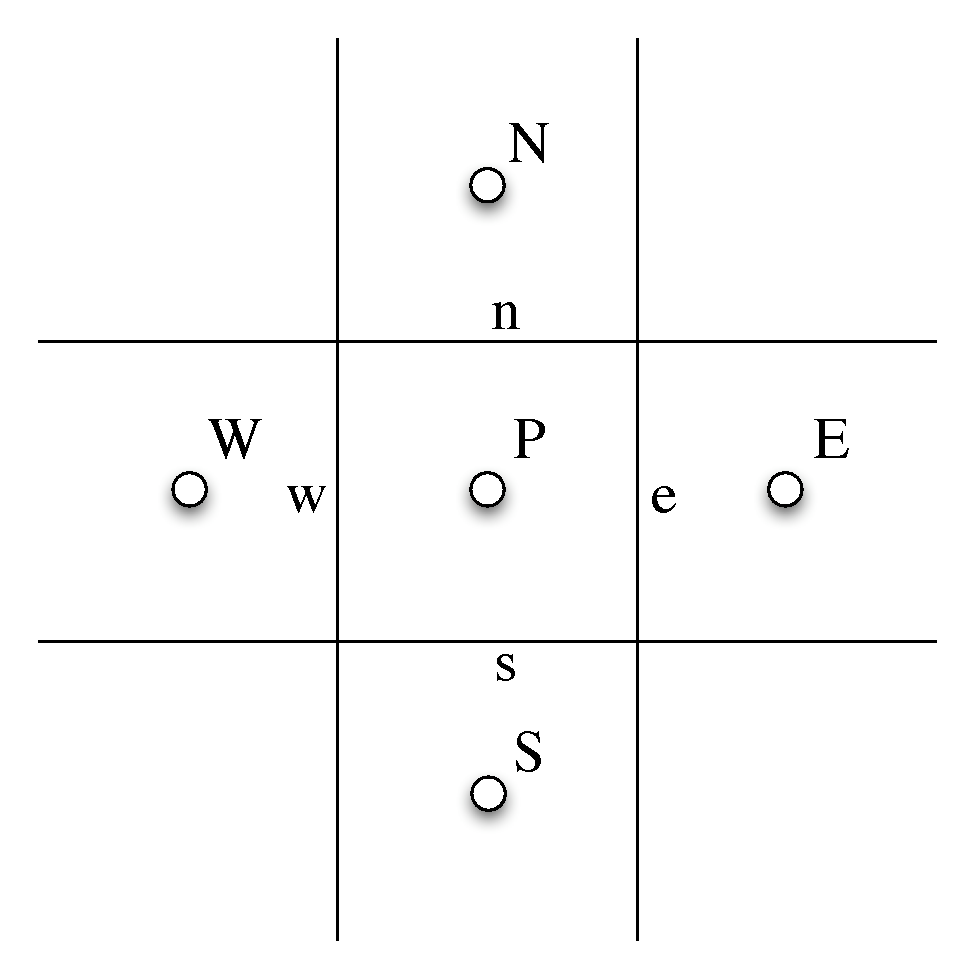
\includegraphics[width=5cm,clip]{index.eps}
\caption{更新セルと参照セルのインデクス}
\label{fig:cell index}
\end{center}
\end{figure}

\begin{equation}
- \frac{1}{h^{\prime}} \sum\limits_{j=1}^{\dim\times2} (-1)^{j} \left( \gamma_{A}\gamma_{BC} q^{\prime} \right)_{j}
\,=\,
\frac{1}{{h^{\prime}}^{2}} \sum\limits_{j=1}^{\dim\times2} \left( \gamma_{A}\gamma_{BC} \lambda \right)_{j} \left( \theta_{J}^{\prime} - \theta_{P}^{\prime} \right)
\,=\,
\frac{1}{{h^{\prime}}^{2}} \left[ \sum\limits_{j=1}^{\dim\times2} \left( \gamma_{A}\gamma_{BC} \lambda \right)_{j} \theta_{J}^{\prime} - 
\theta_{P}^{\prime} \sum\limits_{j=1}^{\dim\times2} \left( \gamma_{A}\gamma_{BC} \lambda \right)_{j} \right]
\label{eq:pscalar semi-discrete4}
\end{equation}

%
\begin{comment}
ここで多媒質の場合,界面における熱伝導率は次式を用いる.

\begin{equation}
\lambda_{j}^{\prime}
\,=\,
{2} \frac{\lambda_{J} \lambda_{P}} {\lambda_{J}^{\prime} + \lambda_{P}}
\label{eq:pscalar semi-discrete5}
\end{equation}
\end{comment}
%

\noindent したがって,\textbf{式(\ref{eq:pscalar semi-discrete2})}は

\begin{equation}
\begin{array}{l}
\displaystyle { \rho^{\prime}C \frac{ {\theta^{\prime}}^{\hspace{0.15em}n+1} - {\theta^{\prime}}^{\hspace{0.15em}n} } {\Delta t^{\prime}}
\,=\, 
-\, \frac{\rho^{\prime}C}{h^{\prime}} \sum\limits_{j=1}^{\dim\times2} {\left( u^{\prime}\,\theta^{\prime} \right)}_j \,n_j^{\prime}
\,+\,
\frac{1}{{h^{\prime}}^{2}} \left[ \sum\limits_{j=1}^{\dim\times2} \left( \gamma_{A}\gamma_{BC} \lambda \right)_{j} \theta_{J}^{\prime} 
\,-\, 
\theta_{P}^{\prime} \sum\limits_{j=1}^{\dim\times2} \left( \gamma_{A}\gamma_{BC} \lambda \right)_{j} \right] }\\
\displaystyle { \qquad \qquad \qquad \quad \,-\,
\frac{1}{h^{\prime}} \sum\limits_{j=1}^{\dim\times2} (-1)^{j} \left\{ \gamma_{A} \left( 1-\gamma_{BC} \right) q_{BC}^{\prime} \right\}_{j} \,+\, Q^{\prime} }
\end{array}
\label{eq:pscalar semi-discrete6}
\end{equation}


\noindent 無次元形式で表示すると,

\begin{equation}
\begin{array}{l}
\displaystyle { \frac{\theta^{\hspace{0.15em}n+1} - \theta^{\hspace{0.15em}n} } {\Delta t}
\, =\, -\, 
\frac{\rho C}{h} \sum\limits_{j=1}^{\dim\times2} {\left( u\,\theta \right)}_j \,n_j }\\
\displaystyle { \, + \,
\frac{1}{h^{2}Pe} \left[ \sum\limits_{j=1}^{\dim\times2} \left( {\gamma_{A}}_{j} {\gamma_{BC}}_{j} \theta_{J} \right)- \theta_{P} \sum\limits_{j=1}^{\dim\times2} {\gamma_{A}}_{j} {\gamma_{BC}}_{j} \right] 
\,-\,
\frac{1}{h} \sum\limits_{j=1}^{\dim\times2} (-1)^{j} \left\{ \left(1-\gamma_{A} \gamma_{BC} \right) q_{BC} \right\}_{j}
\,+\, \Theta_{V} }
\end{array}
\label{eq:pscalar semi-discrete7}
\end{equation}

\noindent ただし,

\begin{equation}
{q}_{BC} \,=\,\frac{q_{BC}^{\prime}} {u_{\mathit{0}}^{\prime} \Delta \theta^{\prime}} \frac{1}{\rho^{\prime}C}
\label{eq:qbc non-dimansionalize}
\end{equation}

である.このとき,無次元化パラメータに用いた$\rho^{\prime},\,C$は解くべき媒質の物性値であることに注意する.C3Dソルバークラスでは,XML入力ファイルにおいて,ReferenceセクションのRef\_IDタグでボクセルIDを指定する.このIDは,SteerセクションのModel\_Settingタグで媒質テーブルと対応づけられ,基礎式で解くべき媒質を示す.つまり,\textbf{式(\ref{eq:qbc non-dimansionalize})}の$\rho^{\prime},\,C$の媒質を示している.


%
\subsection{時間発展方程式}
基礎方程式\textbf{(\ref{eq:passive scalar1 ND})}の対流項を$F$でまとめて表し,時間進行スキームを切り替えるパラメータ$\alpha$を用いると,

\begin{equation}
{\frac{\partial \theta}{\partial t}}^{n+1}
\,=\,
\left({{1}\mathrm{{-}}\mathit{\alpha}}\right){F}^{\hspace{0.33em}{n}}\mathrm{{+}}\mathit{\alpha}{F}^{{n}\mathrm{{+}}{1}}\mathrm{{+}}{\mathrm{\Theta}}_{V}
\label{eq:pscalar evolv2}
\end{equation}

\begin{equation}
\alpha\,=\, \left\{
\begin{array}{cl}
0 & Euler\, Explicit\\
1/2 & Crank\, Nicolson\\
1 & Euler\, Implicit
\end{array} \right.
\label{eq:pscalar evolv3}
\end{equation}

\noindent ソース項の時制については任意性を残しておく.一般に時刻について線形化し,$\Theta_{V}^{\hspace{0.3em}n}$とする方が安定である.以下の議論では,拡散項の時間進行に着目して説明する.

%
\subsubsection{Euler陽解法}

\textbf{式(\ref{eq:pscalar semi-discrete7})}より,

\begin{equation}
\begin{array}{l}
\displaystyle { \frac{{\mathit{\theta}}_{P}^{\hspace{0.3em}{n}\mathrm{{+}}{1}}\mathrm{{-}}{\mathit{\theta}}_{P}^{\hspace{0.3em}{n}}}{\mathrm{\Delta}{t}}
\,=\, -
\frac{\rho C}{h} \sum\limits_{j=1}^{\dim\times2} {\left( u\,\theta \right)}_j \,n_j
\, + \,
\frac{1}{h^{2}Pe} \left[ \sum\limits_{j=1}^{\dim\times2} \left( {\gamma_{A}}_{j} {\gamma_{BC}}_{j} \theta_{J} \right)- \theta_{P} \sum\limits_{j=1}^{\dim\times2} {\gamma_{A}}_{j} {\gamma_{BC}}_{j} \right]^{n} }\\
\displaystyle { \,-\,
\frac{1}{h} \sum\limits_{j=1}^{\dim\times2} (-1)^{j} \left\{ \left(1-\gamma_{A} \gamma_{BC} \right) q_{BC} \right\}_{j}^{n}
\,+\, \Theta_{V}^{\hspace{0.3em}n} }
\end{array}
\label{eq:pscalar ee2}
\end{equation}

\noindent 陽解法の場合には,次の拡散数による数値安定性の点に注意する.
\begin{equation}
\Delta t \,\le\, \frac{1}{2dim}h^{2}Pe
\label{eq:pscalar ee3}
\end{equation}

%
\begin{comment}
\subsection{Euler陰解法}
\begin{equation}
{\frac{\mathrm{\partial}\mathit{\theta}}{\mathrm{\partial}{t}}}^{{n}\mathrm{{+}}{1}}
\,=\,
\mathrm{{-}}{\frac{\mathrm{\partial}{H}_{i}^{n+1}}{\mathrm{\partial}{x}_{i}}}^{n}\,\mathrm{{+}}\,{\mathrm{\Theta}}_{V}^{n}
\label{eq:pscalar ei1}
\end{equation}

\begin{equation}
\frac{{\mathit{\theta}}_{P}^{\hspace{0.33em}{n}\mathrm{{+}}{1}}\mathrm{{-}}{\mathit{\theta}}_{P}^{\hspace{0.33em}{n}}}{\mathrm{\Delta}{t}}\mathrm{{=}}\frac{1}{{h}^{2}Pe}{\left[{\mathop{\sum}\limits_{{j}\mathrm{{=}}{1}}\limits^{\dim\mathrm{\times}{2}}{\left({{\mathit{\gamma}}_{j}{\mathit{\theta}}_{J}}\right)}\mathrm{{-}}{\mathit{\theta}}_{P}\mathop{\sum}\limits_{{j}\mathrm{{=}}{1}}\limits^{\dim\mathrm{\times}{2}}{{\mathit{\gamma}}_{j}}}\right]}^{\hspace{0.33em}{n}\mathrm{{+}}{1}}\mathrm{{-}}\frac{1}{h}\mathop{\sum}\limits_{{j}\mathrm{{=}}{1}}\limits^{\dim\mathrm{\times}{2}}{\left[{{\mathrm{(}}\mathrm{{-}}{1}{\mathrm{)}}^{j}{\left\{{\left({{1}\mathrm{{-}}\mathit{\gamma}}\right){q}_{BC}}\right\}}_{j}^{\hspace{0.33em}{n}\mathrm{{+}}{1}}}\right]}\mathrm{{+}}{\mathrm{\Theta}}_{V}^{\hspace{0.33em}{n}}
\label{eq:pscalar ei2}
\end{equation}

反復式の形で対角項をまとめ,右肩の反復インデクスを$m$とすると,

\begin{equation}
\left[{{1}\mathrm{{+}}\frac{\mathrm{\Delta}{t}}{{h}^{2}Pe}\mathop{\sum}\limits_{{j}\mathrm{{=}}{1}}\limits^{\dim\mathrm{\times}{2}}{{\mathit{\gamma}}_{j}}}\right]{\mathit{\theta}}_{P}^{\hspace{0.33em}{m}\mathrm{{+}}{1}}\mathrm{{=}}{\mathit{\theta}}_{P}^{\hspace{0.33em}{n}}\mathrm{{+}}\frac{\mathrm{\Delta}{t}}{{h}^{2}Pe}\mathop{\sum}\limits_{{j}\mathrm{{=}}{1}}\limits^{\dim\mathrm{\times}{2}}{\left\{{{\mathit{\gamma}}_{j}{\mathit{\theta}}_{J}^{\hspace{0.33em}{m}\mathrm{{+}}{1}}}\right\}}\mathrm{{-}}\frac{\mathrm{\Delta}{t}}{h}\mathop{\sum}\limits_{{j}\mathrm{{=}}{1}}\limits^{\dim\mathrm{\times}{2}}{\left[{{\mathrm{(}}\mathrm{{-}}{1}{\mathrm{)}}^{j}{\left\{{\left({{1}\mathrm{{-}}\mathit{\gamma}}\right){q}_{BC}}\right\}}_{j}^{\hspace{0.33em}{m}}}\right]}\mathrm{{+}}\mathrm{\Delta}{t}\hspace{0.33em}{\mathrm{\Theta}}_{V}^{\hspace{0.33em}{n}}
\label{eq:pscalar ei3}
\end{equation}

右辺第二項の$q_{BC}$は一反復前の値を利用する.ソース項は,前の時刻の値か,あるいは前の反復値を用いる.

%
\subsection{Euler陰解法デルタ形式}
\begin{equation}
\begin{array}{l}
\displaystyle {\left[{{1}\mathrm{{+}}\frac{\mathrm{\Delta}{t}}{{h}^{2}Pe}\mathop{\sum}\limits_{{j}\mathrm{{=}}{1}}\limits^{\dim\mathrm{\times}{2}}{{\mathit{\gamma}}_{j}}}\right]\mathrm{\Delta}{\mathit{\theta}}_{P}^{{m}\mathrm{{+}}{1}}
\,=\,
\frac{\mathrm{\Delta}{t}}{{h}^{2}Pe}\mathop{\sum}\limits_{{j}\mathrm{{=}}{1}}\limits^{\dim\mathrm{\times}{2}}{\left({{\mathit{\gamma}}_{j}{\mathit{\theta}}_{J}^{{m}\mathrm{{+}}{1}}}\right)}\mathrm{{-}}\frac{\mathrm{\Delta}{t}}{h}\mathop{\sum}\limits_{{j}\mathrm{{=}}{1}}\limits^{\dim\mathrm{\times}{2}}{\left[{{\mathrm{(}}\mathrm{{-}}{1}{\mathrm{)}}^{j}{\left\{{\left({{1}\mathrm{{-}}\mathit{\gamma}}\right){q}_{BC}}\right\}}_{j}^{{m}}}\right]}}\\
\qquad \qquad \qquad \qquad \qquad \quad
\displaystyle {\mathrm{{-}}\left[{{1}\mathrm{{+}}\frac{\mathrm{\Delta}{t}}{{h}^{2}Pe}\mathop{\sum}\limits_{{j}\mathrm{{=}}{1}}\limits^{\dim\mathrm{\times}{2}}{{\mathit{\gamma}}_{j}}}\right]{\mathit{\theta}}_{P}^{{n}}\mathrm{{+}}\mathrm{\Delta}{t}{\mathrm{\Theta}}_{V}^{{n}}}
\end{array}
\label{eq:pscalar delta}
\end{equation}

%
\subsection{Crank-Nicolson}

\begin{equation}
{\frac{\mathrm{\partial}\mathit{\theta}}{\mathrm{\partial}{t}}}^{{n}\mathrm{{+}}{1}}
\,=\,
\mathrm{{-}}\frac{1}{2}\left({{\frac{\mathrm{\partial}{H}_{i}^{}}{\mathrm{\partial}{x}_{i}}}^{n}\mathrm{{+}}{\frac{\mathrm{\partial}{H}_{i}^{}}{\mathrm{\partial}{x}_{i}}}^{{n}\mathrm{{+}}{1}}}\right)\mathrm{{+}}{\mathrm{\Theta}}_{V}^{n}
\label{eq:pscalar cn1}
\end{equation}

\begin{equation}
\begin{array}{l}
\displaystyle {\left[{{1}\mathrm{{+}}\frac{\mathrm{\Delta}{t}}{2{h}^{2}Pe}\mathop{\sum}\limits_{{j}\,=\,{1}}\limits^{\dim\mathrm{\times}{2}}{{\mathit{\gamma}}_{j}}}\right]{\mathit{\theta}}_{P}^{{m}\mathrm{{+}}{1}}\,=\,{\mathit{\theta}}_{P}^{{n}}\mathrm{{+}}\frac{\mathrm{\Delta}{t}}{2{h}^{2}Pe}\mathop{\sum}\limits_{{j}\mathrm{{=}}{1}}\limits^{\dim\mathrm{\times}{2}}{\left({{\mathit{\gamma}}_{j}{\mathit{\theta}}_{J}^{{m}\mathrm{{+}}{1}}}\right)}\mathrm{{+}}\frac{\mathrm{\Delta}{t}}{2{h}^{2}Pe}{\left[{\mathop{\sum}\limits_{{j}\,=\,{1}}\limits^{\dim\mathrm{\times}{2}}{\left({{\mathit{\gamma}}_{j}{\mathit{\theta}}_{J}}\right)}\mathrm{{-}}{\mathit{\theta}}_{P}\mathop{\sum}\limits_{{j}\mathrm{{=}}{1}}\limits^{\dim\mathrm{\times}{2}}{{\mathit{\gamma}}_{j}}}\right]}^{{n}}}\\
\qquad \qquad \qquad \qquad \qquad
\displaystyle {\mathrm{{-}}\frac{\mathrm{\Delta}{t}}{2h}\left[{\mathop{\sum}\limits_{{j}\mathrm{{=}}{1}}\limits^{\dim\mathrm{\times}{2}}{\left\{{{\mathrm{(}}\mathrm{{-}}{1}{\mathrm{)}}^{j}{\left({\left({{1}\mathrm{{-}}\mathit{\gamma}}\right){q}_{BC}}\right)}_{j}^{n}}\right\}}}\right.\left.{\mathrm{{+}}\mathop{\sum}\limits_{{j}\mathrm{{=}}{1}}\limits^{\dim\mathrm{\times}{2}}{\left\{{{\mathrm{(}}\mathrm{{-}}{1}{\mathrm{)}}^{j}{\left({\left({{1}\mathrm{{-}}\mathit{\gamma}}\right){q}_{BC}}\right)}_{j}^{{m}}}\right\}}}\right]\mathrm{{+}}\mathrm{\Delta}{t}{\mathrm{\Theta}}_{V}^{{n}}}
\end{array}
\label{eq:pscalar cn2}
\end{equation}

%
\subsection{定常解}
\textbf{式(\ref{eq:pscalar evolv4})}を定常状態として計算する場合には,次式を解く.

\begin{equation}
{\mathit{\theta}}_{P}^{{m}\mathrm{{+}}{1}}
\,=\,
{\left[{\mathop{\sum}\limits_{{j}\mathrm{{=}}{1}}\limits^{\dim\mathrm{\times}{2}}{{\mathit{\gamma}}_{j}}}\right]}^{\mathrm{{-}}{1}}\left[{\mathop{\sum}\limits_{{j}\mathrm{{=}}{1}}\limits^{\dim\mathrm{\times}{2}}{\left({{\mathit{\gamma}}_{j}{\mathit{\theta}}_{J}^{{m}\mathrm{{+}}{1}}}\right)}\mathrm{{-}}{hPe}\mathop{\sum}\limits_{{j}\mathrm{{=}}{1}}\limits^{\dim\mathrm{\times}{2}}{\left\{{{\mathrm{(}}\mathrm{{-}}{1}{\mathrm{)}}^{j}{\left({\left({{1}\mathrm{{-}}\mathit{\gamma}}\right){q}_{BC}}\right)}_{j}^{{m}}}\right\}}\mathrm{{-}}{h}^{2}{Pe}{\mathrm{\Theta}}_{V}^{{n}}}\right]
\label{eq:pscalar steady}
\end{equation}

この場合$\gamma$の状況により対角項の係数がゼロになる場合が生じる.この問題点を回避するために,圧力の場合と同様に$\varepsilon$を導入する.

\begin{equation}
{\mathit{\theta}}_{P}^{{m}\mathrm{{+}}{1}}
\,=\,
{\left[{\mathrm{\varepsilon}\mathrm{{+}}\mathop{\sum}\limits_{{j}\mathrm{{=}}{1}}\limits^{\dim\mathrm{\times}{2}}{{\mathit{\gamma}}_{j}}}\right]}^{\mathrm{{-}}{1}}\left[{\mathop{\sum}\limits_{{j}\mathrm{{=}}{1}}\limits^{\dim\mathrm{\times}{2}}{\left({{\mathit{\gamma}}_{j}{\mathit{\theta}}_{J}^{{m}\mathrm{{+}}{1}}}\right)}\mathrm{{-}}{hPe}\mathop{\sum}\limits_{{j}\mathrm{{=}}{1}}\limits^{\dim\mathrm{\times}{2}}{\left\{{{\mathrm{(}}\mathrm{{-}}{1}{\mathrm{)}}^{j}{\left({\left({{1}\mathrm{{-}}\mathit{\gamma}}\right){q}_{BC}}\right)}_{j}^{{m}}}\right\}}\mathrm{{-}}{h}^{2}{Pe}{\mathrm{\Theta}}_{V}^{{n}}}\right]
\label{eq:pscalar steady2}
\end{equation}

\end{comment}



%
\subsection{セル界面に対する熱境界条件}
本節で述べる熱境界条件を\textbf{式(\ref{eq:pscalar semi-discrete6})}の$q_{BC}^{\prime}$に代入することにより,多様な熱境界条件を導入することができる.熱流束の次元は,

\begin{equation}
q_{BC}^{\prime}\, \sim \, - \lambda \frac{\partial \theta^{\prime}}{\partial {x_{i}}^{\prime}} \qquad [W/m^2]
\label{eq:pscalar qbc}
\end{equation}

\noindent 境界条件に必要なパラメータは多媒質への拡張も考慮し,有次元での入力とする.
熱流束形式の境界条件は,前の時刻あるいは前の反復ステップの値を用いて,流束の形式で計算しておき,その値を反復過程で参照しながら計算する.


%
\subsubsection{熱流束境界 $q_D$}
何らかの物理モデルにより,熱流束$q'\,[W/m^2]$が直接与えられる場合に用いる.
セル界面における熱流束 $q_{i+1/2}' > 0$が与えられた場合を考える.熱流の方向が正なので,セル $i$ は冷却,セル $i+1$ は加熱となる.
単媒質の場合,

\begin{equation}
{q}_{D} \,=\, \frac{q_{D}^{\prime}}{{u_{\mathit{0}}}^{\prime} \Delta \theta^{\prime}} \frac{1}{\rho^{\prime}C}
\label{eq:qD}
\end{equation}

\noindent ここで$\rho^{\prime}C$は解くべきセルの物性値で,単媒質の場合には予め定数として与えられる.
次の例では,ID=78とID=1で挟まれる面に$q_{D}'=2.0\, [W/m^2]$の熱流束を与えている.
\begin{indentation}{3zw}{0zw}
{
\small
\begin{program}
<Elem name="Direct" id="78" comment="direct_1">
  <Param name="def_face"  dtype="INT"  value="1" />
  <Param name="Heat_Flux" dtype="REAL" value="2.0"/>
</Elem>
\end{program}
}
\end{indentation}

%
\subsubsection{熱伝達境界 $q_T$}
\label{sec:Heat_Transfer_BC}
熱伝達形式の境界熱流束は,下記のように書ける.

\begin{equation}
{q}_{T}^{\prime} \,=\, -H(\theta_{sf}^{\prime}\,-\,\theta_{\infty}^{\prime})
\label{eq:qT2}
\end{equation}

\begin{center}
\begin{tabular}{lll}
$H$ &  $[W\,/\,(m^2K)]$ & Coefficient\, of\, heat\, transfer\\
$\theta_{sf}^{\prime}$ & $[K]$ & Surface\, temperature\, of\, solid\\
$\theta_{\infty}^{\prime}$ & $[K]$ & Temperature\, at\, outer\, boundary\, layer\\
\end{tabular}
\end{center}

\textbf{図\ref{fig:heat transfer on solid}}において,セルPにおける熱量の収支を考える.セルPは固体壁Sとの界面で正の熱流束が与えられたときにセルの温度が上昇する.
一般に外部流の場合には,温度境界層外縁における参照温度$\theta_{\infty}^{\prime}$は,セル幅が温度境界層よりも厚い場合を想定しているので,P点の温度としてよい.
しかしながら,複雑な流動となる内部流の場合には参照温度自体の定義に一意性がない.参照温度として外部流のようにP点をとると,温度差が小さくなる場合に熱伝達による熱流束が小さくなる.一方で,基準温度を想定すると,局所的な温度分布に関係なく一定量の熱伝達流束を与えることになる点に注意する.

固体表面における温度が必要な場合には,等間隔格子上で,

\begin{equation}
\theta_{sf}^{\prime} \,=\, \frac{\lambda_{S} \theta_{S} + \lambda_{P} \theta_{P}}{\lambda_{S} + \lambda_{P}}
\label{eq:qT3}
\end{equation}

\noindent となる.\textbf{表\ref{tbl:medium property}}に示すように固体の熱伝導率は流体よりも大きい$( \lambda_{solid}\, \gg \, \lambda_{fluid} )$ ため,一般に$\theta_{sf}^{\prime} \cong \theta_{solid}^{\prime}$のように考えてよい.

\begin{figure}[htdp]
\begin{center}
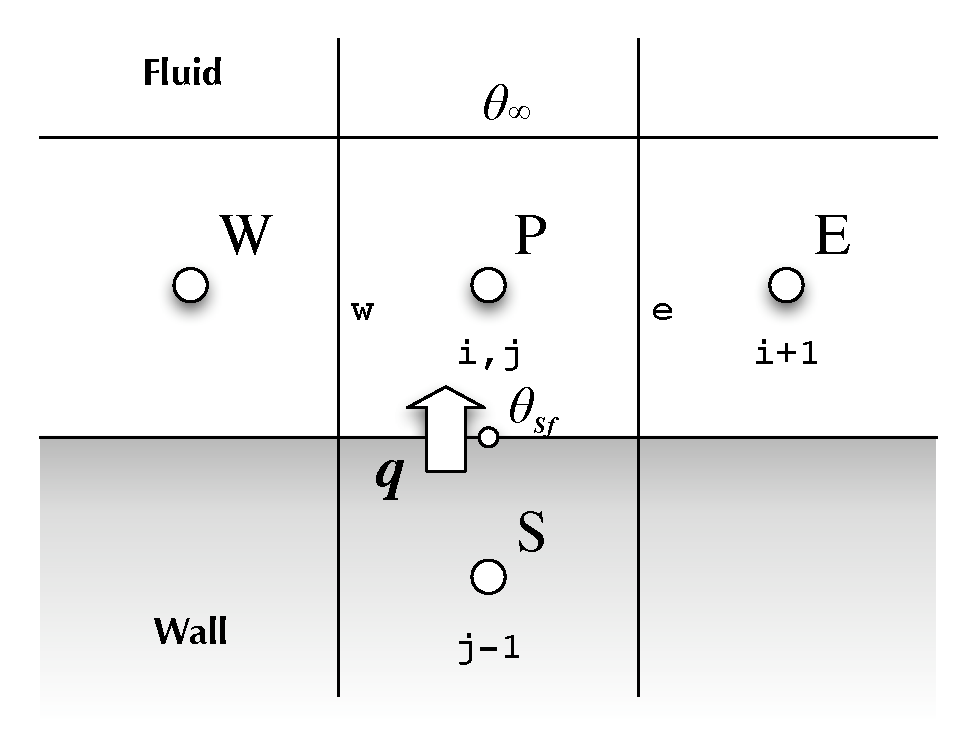
\includegraphics[width=6cm,clip]{HeatTransfer.eps}
\caption{固体壁面での熱伝達}
\label{fig:heat transfer on solid}
\end{center}
\end{figure}

指定面における熱伝達境界条件の実装方法として,次の3つの場合が考えられる.
\begin{indentation}{3zw}{0zw}
\begin{description}
\item[タイプ N)] 熱伝達係数を与え,計算結果の固体表面温度から熱流束を計算する.共役熱移動の場合に利用する.
\item[タイプ S)] 表面温度と熱伝達係数を与え,熱流束を計算する.流体のみを解く場合に利用する.
\item[タイプ B)] 熱伝達係数とバルク温度を与え,熱流束を計算する.固体の熱移動のみを解く場合の境界条件として利用する.
\item[タイプ SNB/SNL)] 自然対流の乱流熱伝達の実験式を実装したもの.流体のみを解く場合に利用し,タイプSを拡張している.SNBは温度差の定義にバルク温度を用い,SNLは隣接セルの値を用いた実装である.
\item[タイプ SFB/SFL)] 強制対流の層流・乱流熱伝達の実験式を実装したもの.流体のみを解く場合に利用し,タイプSを拡張している.SFBは温度差の定義にバルク温度を用い,SFLは隣接セルの値を用いた実装である.
\end{description}
\end{indentation}

%
\paragraph{Nusselt数とStanton数}
まず,ヌセルト数との関連を示す.ヌセルト数の定義は,熱伝導に対する熱伝達の比なので,

\begin{equation}
Nu \,=\, \frac{HL^{\prime}}{\lambda}, \qquad \left.
\begin{array}{ll}
H & [W/(m^2K)]\\
\lambda & [W/(mK)]\\
L^\prime & [m]
\end{array} \right\}
\label{eq:nu_1}
\end{equation}

フーリエの法則とニュートンの冷却則から,

\begin{equation}
{H} \,=\, \lambda {\left({\frac{\mathrm{\partial}{\mathit{\theta}}'}{\mathrm{\partial}{n}'}}\right)}_{{n}'\mathrm{{=}}{0}}\, \Bigg/ {\mathrm{\Delta}{\mathit{\theta}}'}
\,=\,
\frac{{\mathit{\lambda}}\mathrm{\Delta}{\mathit{\theta}}'}{{L}'\mathrm{\Delta}{\mathit{\theta}}'}{\left({\frac{\mathrm{\partial}\mathit{\theta}}{\mathrm{\partial}{n}}}\right)}_{{n}\mathrm{{=}}{0}}
\,=\,
\frac{{\mathit{\lambda}}}{{L}'}{\left({\frac{\mathrm{\partial}\mathit{\theta}}{\mathrm{\partial}{n}}}\right)}_{{n}\mathrm{{=}}{0}}
\label{eq:nu_2}
\end{equation}

\begin{equation}
Nu \,=\, \left( \frac{\partial \theta}{\partial n} \right)_{n=0}
\label{eq:nu_3}
\end{equation}

一方,熱流束を表す\textbf{式(\ref{eq:pscalar qbc})}の無次元形式は,\textbf{式(\ref{eq:qD})}となり,これはStanton数を表す.つまり,

\begin{equation}
q \,=\, \frac{q^\prime}{u_{\mathit 0}^\prime \Delta \theta^\prime} \frac{1}{\rho^\prime C}
\quad \equiv \quad 
St\,=\, \frac{Nu}{Re Pr} 
\label{eq:stanton}
\end{equation}


%
\paragraph{タイプ N}
タイプNの計算は固体表面セルの温度は計算によって決まる値を用い,熱伝達係数($H>0$)のみで計算できる.\textbf{図\ref{fig:typeN}}には,固体と流体の相対的な位置が異なる(a), (b)2つのパターンを示している.いま,セル境界において,正の熱流束$q_{j+1/2}^{\prime}>0$を仮定する.つまり,

\begin{equation}
q_{j+1/2}^{\prime}\,=\,-H(\theta_{j+1}^{\prime}-\theta_{j}^{\prime})\, >\,0 \quad \Longleftrightarrow \quad \theta_{j}^{\prime} \,>\, \theta_{j+1}^{\prime}
\label{eq:qT_N1}
\end{equation}

$q_{j+1/2}^{\prime}>0$なので,jセルは冷却, j+1セルは加熱となる.次に,セル界面において負の熱流束$q_{j+1/2}^{\prime}<0$を仮定すると,

\begin{equation}
q_{j+1/2}^{\prime} \,=\,-H(\theta_{j+1}^{\prime}-\theta_{j}^{\prime})\, <\,0 \quad \Longleftrightarrow \quad \theta_{j}^{\prime} \,<\, \theta_{j+1}^{\prime}
\label{eq:qT_N2}
\end{equation}

したがって,熱伝達形式の境界熱流束$q_{T}'$は,常に次式で計算できる.

\begin{equation}
q_{T,\,j+1/2}^{\prime} \,=\,-H(\theta_{j+1}^{\prime}-\theta_{j}^{\prime})
\label{eq:qT_N3}
\end{equation}

\textbf{式(\ref{eq:qbc non-dimansionalize})}を用いて無次元化すると,

\begin{equation}
q_{T,\,j+1/2} \,=\, - \frac{1}{\rho^{\prime} C} \frac{H}{{u_{\mathit{0}}}^{\prime}}(\theta_{j+1}-\theta_{j})
\label{eq:qT_N4}
\end{equation}

ここで$\rho^{\prime}C$は,単媒質の場合には代表媒質の物性値である.

\begin{figure}[htdp]
\begin{center}
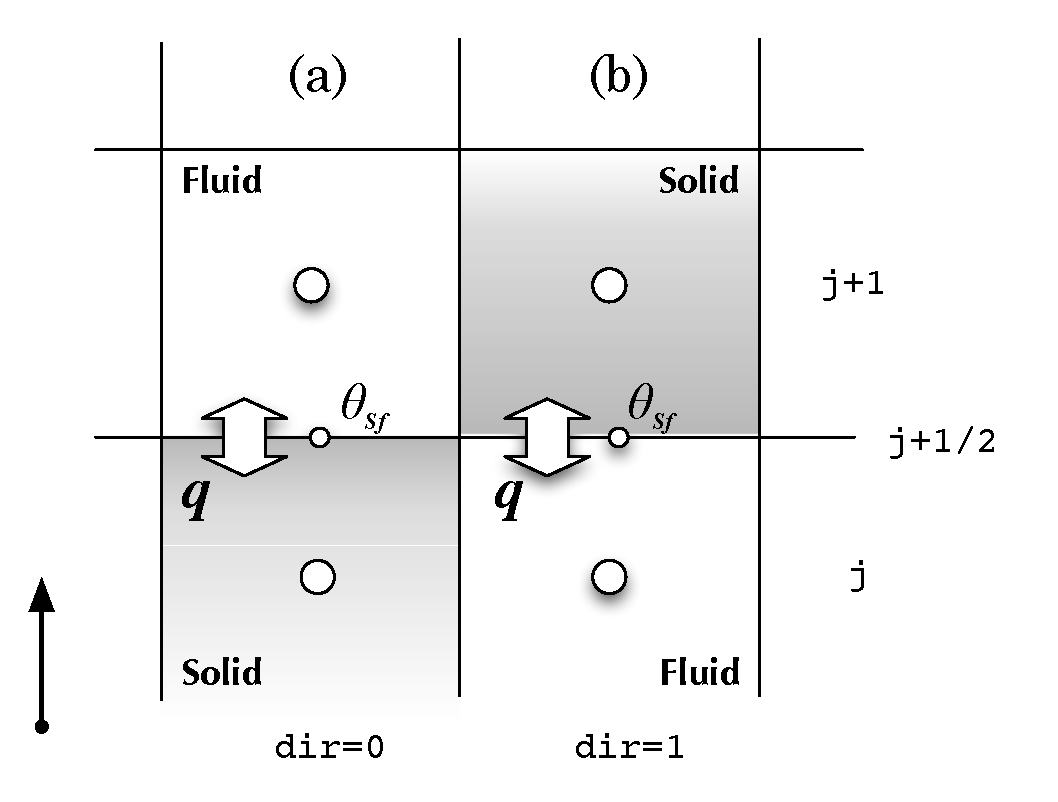
\includegraphics[width=7cm,clip]{typeN.eps}
\caption{熱伝達境界タイプN/Sのパターン.方向フラグdirは\textbf{式(\ref{eq:qT_S1})}で用いるインデクスjに対する相対的な位置を示す.}
\label{fig:typeN}
\end{center}
\end{figure}

\begin{indentation}{3zw}{0zw}
{
\small
\begin{program}
<Elem name="Heat_Transfer_N" id="68"  comment="HF_1">
  <Param name="def_face"    dtype="INT"    value="1" />
  <Param name="Coef_of_Heat_Transfer" dtype="REAL" value="1.2e-2"/>
</Elem>
\end{program}
}
\end{indentation}

%
\paragraph{タイプ S}
この境界条件は想定する表面温度と熱伝達係数を与える.熱流体計算で固体側を解かず,流体のみを解く場合の境界条件として用いる.
\textbf{図\ref{fig:typeN}}を参照して,参照温度を外側1点目にとる場合,パターン(a)の$dir=0$のときに法線が正になるようにインデクス計算を行うと,

\begin{equation}
q_{T,\,j+1/2} \,=\, - \frac{1}{\rho^{\prime}C} \frac{H}{{u_{\mathit{0}}}^{\prime}} \left( \theta_{j+1-dir} -\theta_{sf} \right) \left( 1-2{dir} \right)
\label{eq:qT_S1}
\end{equation}

\noindent また,参照温度を基準温度にとる場合,
\begin{equation}
q_{T,\,j+1/2} \,=\, - \frac{1}{\rho^{\prime}C} \frac{H}{{u_{\mathit{0}}}^{\prime}} \left( \theta_0 -\theta_{sf} \right) \left( 1-2{dir} \right)
\label{eq:qT_S1_2}
\end{equation}

\noindent タイプSの実装は,\textbf{式(\ref{eq:qT_S1_2})}である.

次の例では,ID=67に80度の温度が与えられ,ID=1と挟まれる面に熱伝達係数$H=0.012\, [W/(m^{2}K)]$が与えられる.

\begin{indentation}{3zw}{0zw}
{
\small
\begin{program}
<Elem name="Heat_Transfer_S" id="67"  comment="HF_2">
  <Param name="def_face"    dtype="INT"    value="1" />
  <Param name="Surface_Temperature" dtype="REAL" value="80.0"/>
  <Param name="Coef_of_Heat_Transfer" dtype="REAL" value="1.2e-2"/>
</Elem>
\end{program}
}
\end{indentation}

%
\paragraph{タイプ B}
この境界条件は固体熱伝導を解く場合の境界条件である.つまり,固体セルのみを解き,流体セルは解かない場合に用い,流体の参照温度と熱伝達係数を指定する.計算式は\textbf{式(\ref{eq:qT_B1})}を用いる.参照する流体のインデクスは,\textbf{図\ref{fig:typeB}}のように,タイプN/S と参照方向が逆になっている.パターン(a)の場合に熱伝達面からの法線は正,(b)の場合に法線が負になるように,方向を表すインデクス計算を$2dir-1$として,

\begin{equation}
q_{T,\,j+1/2} \,=\, \frac{1}{\rho^{\prime}C} \frac{H}{{u_{\mathit{0}}}^{\prime}} \left( \theta_{j+1-dir} -\theta_{\infty} \right) \left( 2{dir} -1\right)
\label{eq:qT_B1}
\end{equation}

次の例では,ID=60に10度の温度が与えられ,ID=1と挟まれる面に熱伝達係数$H=0.2\, [W/(m^{2}K)]$が与えられる.

\begin{indentation}{3zw}{0zw}
{
\small
\begin{program}
<Elem name="Heat_Transfer_B" id="60"  comment="HF_3">
  <Param name="def_face"    dtype="INT"    value="1" />
  <Param name="Bulk_Temperature" dtype="REAL" value="10.0"/>
  <Param name="Coef_of_Heat_Transfer" dtype="REAL" value="0.2"/>
</Elem>
\end{program}
}
\end{indentation}

\begin{figure}[htdp]
\begin{center}
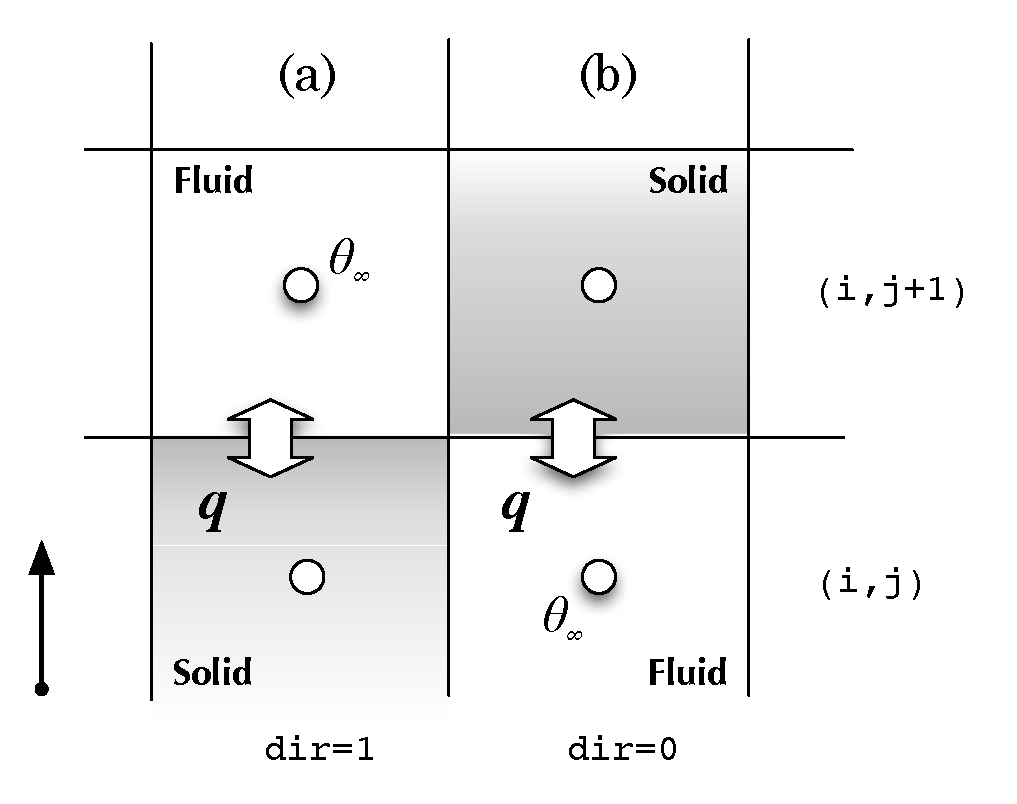
\includegraphics[width=7cm,clip]{typeB.eps}
\caption{熱伝達境界Bのパターン.}
\label{fig:typeB}
\end{center}
\end{figure}



%
\paragraph{タイプ SNB/SNL}
文献\cite{shouji:95:Dennetsu}には,平板に対する自然対流の層流と乱流の熱伝達に関する近似式が説明されている.雰囲気流体の温度に比べ加熱面の温度が非常に高い場合,平板が長くなると境界層が不安定になり,ほぼ$Ra>10^9$で層流から乱流へ遷移する.垂直平板に関する平均熱伝達$(\overline{Nu_L},代表長L)$は次式で整理される.

\begin{equation}
\left.
\begin{array}{lll}
\vspace{1mm}
層流 & \overline{Nu_L} \,=\, 0.59Ra_L^{1/4} & (10^4 < Ra_L < 10^9)\\
乱流 & \overline{Nu_L} \,=\, 0.10Ra_L^{1/3} & (10^9 < Ra_L < 10^{13})
\end{array} \right\}
\label{eq:natural_convection_vert_ht}
\end{equation}

一方,水平平板の場合には,加熱面が上面と下面にある場合で雰囲気流体の挙動が異なるため,\textbf{式(\ref{eq:natural_convection_horiz_ht})}のように整理されている.

\begin{equation}
\left.
\begin{array}{lll}
\vspace{1mm}
上面加熱 & \overline{Nu_L} \,=\, 0.54Ra_L^{1/4} & (10^4 < Ra_L < 10^7)\\
\vspace{1mm}
上面加熱 & \overline{Nu_L} \,=\, 0.15Ra_L^{1/3} & (10^7 < Ra_L < 10^{11})\\
\vspace{1mm}
下面加熱 & \overline{Nu_L} \,=\, 0.27Ra_L^{1/4} & (10^5 < Ra_L < 10^{10})
\end{array} \right\}
\label{eq:natural_convection_horiz_ht}
\end{equation}

\noindent 上記の自然対流熱伝達の整理式を\textbf{図\ref{fig:natural_heat_transfer}}に示す.\\

\begin{figure}[htdp]
\begin{center}
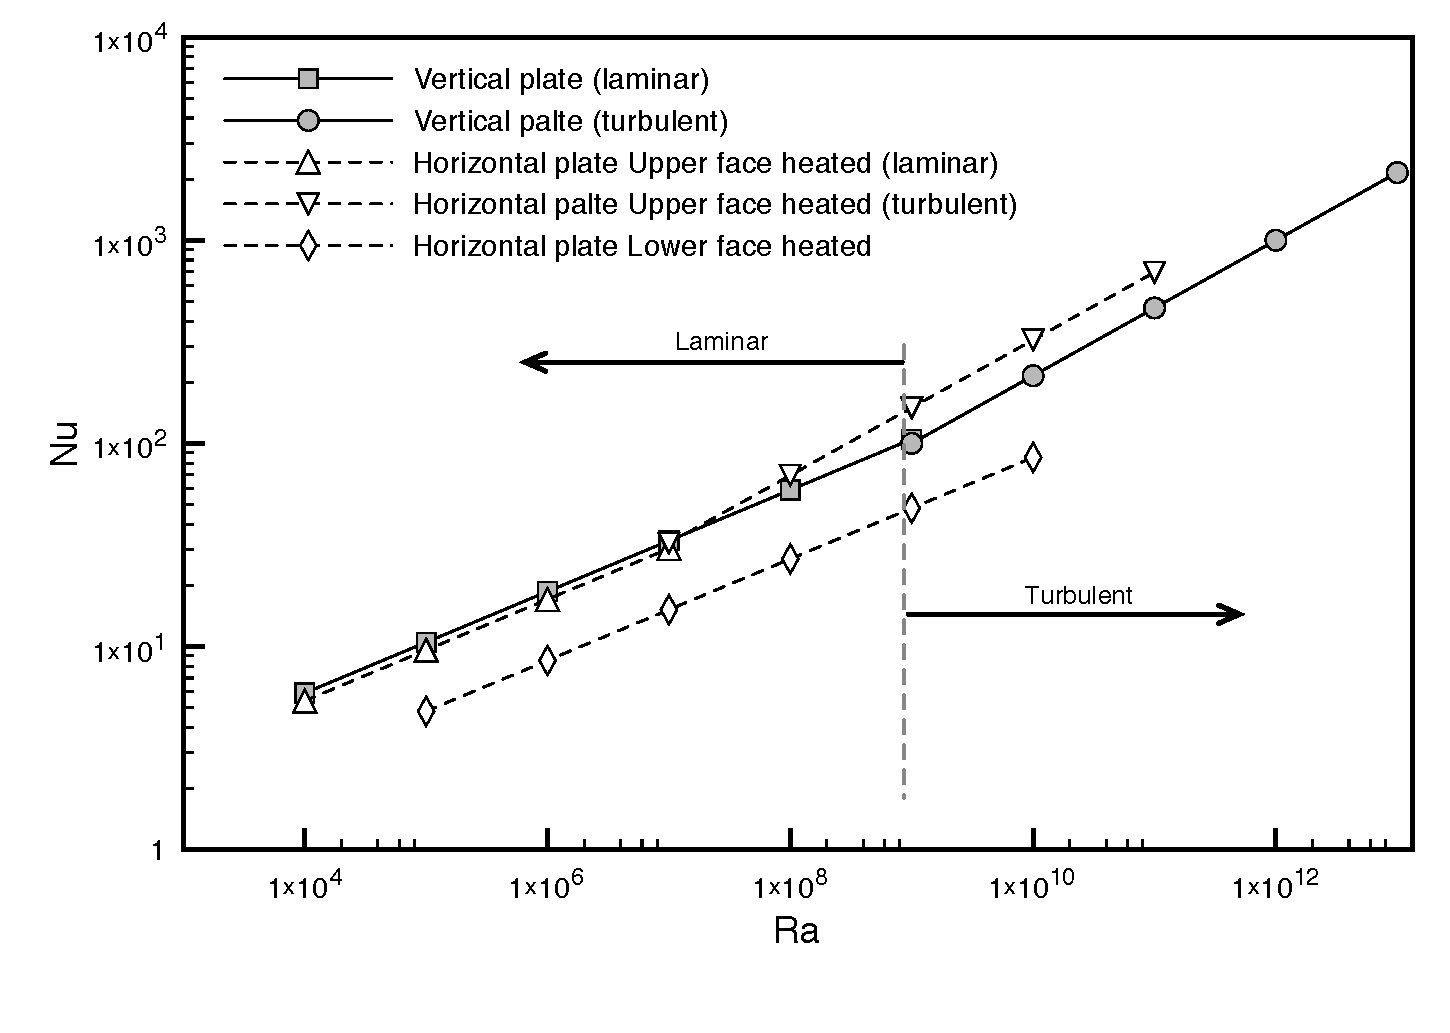
\includegraphics[width=12cm,clip]{HeatTransfer_Natural.eps}
\caption{自然対流熱伝達の整理式\cite{shouji:95:Dennetsu}}
\label{fig:natural_heat_transfer}
\end{center}
\end{figure}

これらの整理式を見ると,大まかには垂直面の実験式を用いて水平面の上面を近似できると考える.そこで,水平面の上面と垂直面,水平面の下面の2つのパターンについて,層流と乱流の実験式を用いることにする.境界条件のパラメータで与える値を\textbf{表\ref{tbl:heat transfer type SN para}}に示す.標準的には,\textbf{式(\ref{eq:natural_convection_vert_ht})}, \textbf{式(\ref{eq:natural_convection_horiz_ht})}の値を用いる.

\begin{table}[htdp]
\caption{自然対流熱伝達のパラメータ}
\begin{center}
\small
\begin{tabular}{ll}\toprule
パラメータタグ & 記号の意味\\ \midrule
vertival\_laminar\_alpha & 垂直平板の層流時の係数$\alpha$\\
vertival\_laminar\_beta & 垂直平板の層流時の係数$\beta$\\
vertival\_turbulent\_alpha & 垂直平板の乱流時の係数$\alpha$\\
vertival\_turbulent\_beta & 垂直平板の乱流時の係数$\beta$\\
vertival\_Ra\_critial & 垂直平板の臨界Ra数$Ra_L$\\
lower\_laminar\_alpha & 水平平板(下面)の層流時の係数$\alpha$\\
lower\_laminar\_beta & 水平平板(下面)の層流時の係数$\beta$\\
lower\_turbulent\_alpha & 水平平板(下面)の乱流時の係数$\alpha$\\
lower\_turbulent\_beta & 水平平板(下面)の乱流時の係数$\beta$\\
lower\_Ra\_critial & 水平平板(下面)の臨界Ra数$Ra_L$\\ 
type & BULK\_TEMPERATURE or LOCAL\_TEMPERATURE\\ \bottomrule
\end{tabular}
\end{center}
\label{tbl:heat transfer type SN para}
\end{table}

次に,タイプSNの熱伝達境界条件の実装について説明する.\textbf{式(\ref{eq:natural_convection_vert_ht})},\textbf{式(\ref{eq:natural_convection_horiz_ht})}は形式的に次式のように表せる.

\begin{equation}
\overline{Nu_L} \,=\, \alpha {Ra_L}^{\,\beta}
\label{eq:typeSN_form}
\end{equation}

\noindent \textbf{式(\ref{eq:nu_1})}と\textbf{式(\ref{eq:typeSN_form})}から,

\begin{equation}
H \,=\, \alpha Ra_L^\beta \frac{\lambda}{L^\prime}
\label{eq:typeSN_form_ht}
\end{equation}

\noindent \textbf{式(\ref{eq:qT2})}と\textbf{式(\ref{eq:qbc non-dimansionalize})}から,

\begin{equation}
q \,=\, - \frac{q^\prime}{{u_\mathit{0}}^\prime \Delta \theta^\prime \rho^\prime C}
\,=\, - \frac{H (\theta_{sf}\,-\,\theta_\infty)}{{u_\mathit{0}}^\prime \rho^\prime C}
\,=\, - \frac{\lambda (\theta_{sf}\,-\,\theta_\infty)}{{u_\mathit{0}}^\prime L^\prime \rho^\prime C} \, \alpha Ra_L^\beta
\label{eq:typeSN_heat_flux}
\end{equation}

\noindent ここで,水平面の上下面では熱伝達が大きく異なるので,z軸方向が重力方向と仮定して,上下面で選択的な実装を行う.上下面の選択は\textbf{図\ref{fig:typeN}}から,

\begin{equation}
\left.
\begin{array}{ll}
\vspace{1mm}
上面加熱 & dir=0\\
\vspace{1mm}
下面加熱 & dir=1
\end{array} \right\}
\label{eq:selection of face}
\end{equation}

\subparagraph{SNL}
\noindent 参照点をひとつ外側の点にとるタイプSNLの場合,パラメータにLOCAL\_TEMPERATUREを指定する.
\textbf{式(\ref{eq:selection of face})}の関係を用いて,\textbf{式(\ref{eq:qT_S1})}に倣い,

\begin{equation}
q_{T,\,j+1/2} \,=\, - \frac{\lambda \left( \theta_{j+1-dir} -\theta_{sf} \right)}{{u_\mathit{0}}^\prime L^\prime \rho^\prime C} \, \alpha Ra_L^\beta \, \left( 1-2{dir} \right)
\label{eq:typeSN_heat_flux_ND}
\end{equation}

\subparagraph{SNB}
参照点を基準温度(BaseTmp)にとるSNBの場合,BULK\_TEMPERATUREを指定する.

\begin{equation}
q_{T,\,j+1/2} \,=\, - \frac{\lambda \left( \theta_0 -\theta_{sf} \right)}{{u_\mathit{0}}^\prime L^\prime \rho^\prime C} \, \alpha Ra_L^\beta \, \left( 1-2{dir} \right)
\label{eq:typeSN_heat_flux_ND_2}
\end{equation}


次の例では,ID=67に80度の温度が与えられ,ID=1と挟まれる面に\textbf{式(\ref{eq:natural_convection_vert_ht})},\textbf{(\ref{eq:natural_convection_horiz_ht})}の熱伝達係数が与えられる.

\begin{indentation}{3zw}{0zw}
\small
\begin{program}
<Elem name="Heat_Transfer_SN" id="67"  comment="HF_2">
  <Param name="def_face"    dtype="INT"    value="1" />
  <Param name="type"    dtype="STRING"    value="BULK_TEMPERATURE" />
  <Param name="Surface_Temperature" dtype="REAL" value="80.0"/>
  <Param name="vertival_laminar_alpha" dtype="REAL" value="0.59"/>
  <Param name="vertival_laminar_beta"  dtype="REAL" value="0.25"/>
  <Param name="vertival_turbulent_alpha" dtype="REAL" value="0.1"/>
  <Param name="vertival_turbulent_beta"  dtype="REAL" value="0.3333333"/>
  <Param name="vertival_ra_critial" dtype="REAL" value="1.0e9"/>
  <Param name="lower_laminar_alpha" dtype="REAL" value="0.27"/>
  <Param name="lower_laminar_beta"  dtype="REAL" value="0.25"/>
  <Param name="lower_turbulent_alpha" dtype="REAL" value="0.27"/>
  <Param name="lower_turbulent_beta"  dtype="REAL" value="0.25"/>
  <Param name="lower_ra_critial" dtype="REAL" value="1.0e9"/>
</Elem>
\end{program}
\end{indentation}

%
\paragraph{タイプ SFB/SFL}
強制対流熱伝達の実験式を組み込んだ熱伝達境界条件を与える.
文献\cite{shouji:95:Dennetsu}から,平板に対する発達した強制対流の乱流熱伝達は,実験による摩擦係数の測定結果とチルトン-コルバーンのアナロジーを用い,温度一定で平板が遷移長さよりも十分に大きいと仮定すると,\textbf{式(\ref{eq:forced_convection_ht})}のように表せる.\textbf{図\ref{fig:forced_heat_transfer}}には幾つかの$Pr$数に対する熱伝達の様子を示す.

\begin{equation}
\overline{Nu_L} \,=\, 0.037Re_L^{4/5}Pr^{1/3}
\label{eq:forced_convection_ht}
\end{equation}

\begin{figure}[htdp]
\begin{center}
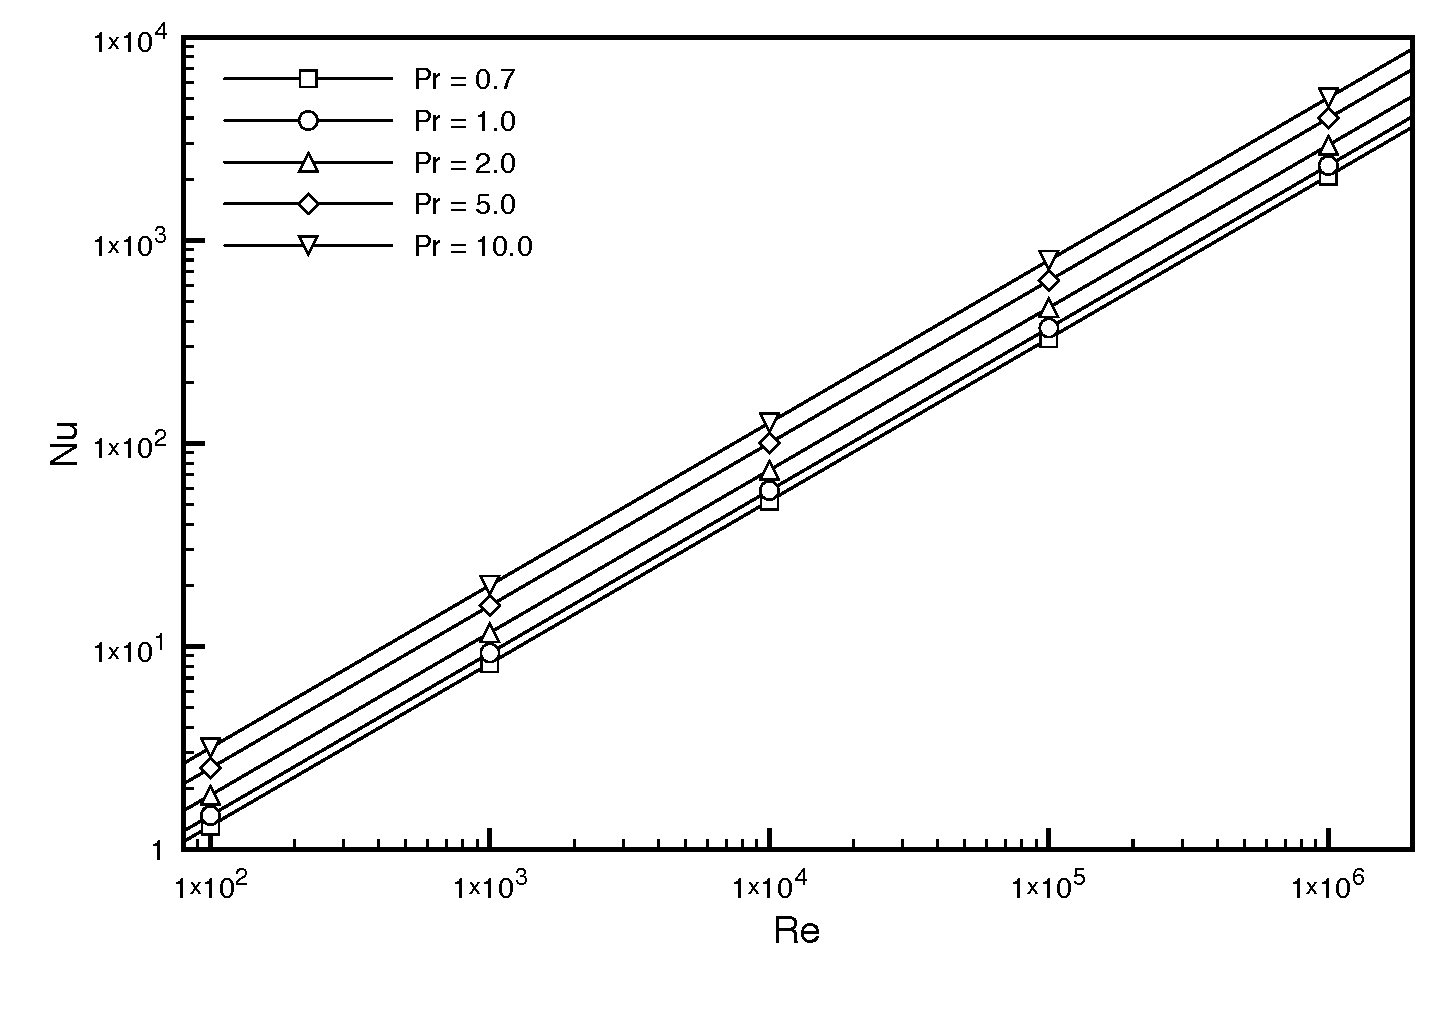
\includegraphics[width=12cm,clip]{HeatTransfer_Forced.eps}
\caption{強制対流熱伝達\cite{shouji:95:Dennetsu}}
\label{fig:forced_heat_transfer}
\end{center}
\end{figure}

\noindent 熱伝達係数の形式を次のように表し,タイプSNと同様に書き下すと,

\begin{equation}
H \,=\, \alpha Re_L^\beta \, Pr^\gamma \, \frac{\lambda}{L^\prime}
\label{eq:typeSF_form_ht}
\end{equation}

タイプSNと同様に,\textbf{式(\ref{eq:typeSF_form_ht})}のパラメータを\textbf{表\ref{tbl:heat transfer type SF para}}で与える.

\begin{table}[htdp]
\caption{強制対流熱伝達のパラメータ}
\begin{center}
\small
\begin{tabular}{ll}\toprule
パラメータタグ & 記号の意味\\ \midrule
alpha & 係数$\alpha$\\
beta & 係数$\beta$\\
gamma & 係数$\gamma$\\
type & BULK\_TEMPERATURE or LOCAL\_TEMPERATURE\\ \bottomrule
\end{tabular}
\end{center}
\label{tbl:heat transfer type SF para}
\end{table}

次に,タイプSFの熱伝達境界条件の実装について説明する.\textbf{式(\ref{eq:typeSF_form_ht})}は温度差の取り方により,次の2つのタイプがある.

\subparagraph{SFL}
参照点を一つ外側にとる場合,パラメータにLOCAL\_TEMPERATUREを指定する.
\begin{equation}
q_{T,\,j+1/2} \,=\, - \frac{\lambda \left( \theta_{j+1-dir} -\theta_{sf} \right)}{{u_\mathit{0}}^\prime L^\prime \rho^\prime C} \, \alpha Re_L^\beta \, Pr^\gamma \,\left( 1-2{dir} \right)
\label{eq:typeSF_heat_flux_ND}
\end{equation}

\subparagraph{SFB}
参照点を基準温度(BaseTmp)にとるSFBの場合,BULK\_TEMPERATUREを指定する.
\begin{equation}
q_{T,\,j+1/2} \,=\, - \frac{\lambda \left( \theta_0 -\theta_{sf} \right)}{{u_\mathit{0}}^\prime L^\prime \rho^\prime C} \, \alpha Re_L^\beta \, Pr^\gamma \,\left( 1-2{dir} \right)
\label{eq:typeSF_heat_flux_ND_2}
\end{equation}


次の例では,ID=60に80度の温度が与えられ,ID=1と挟まれる面に\textbf{式(\ref{eq:forced_convection_ht})}の熱伝達係数が与えられる.

\begin{indentation}{3zw}{0zw}
\small
\begin{program}
<Elem name="Heat_Transfer_SF" id="60"  comment="HF_3">
  <Param name="def_face"    dtype="INT"    value="1" />
  <Param name="type"    dtype="STRING"    value="LOCAL_TEMPERATURE" />
  <Param name="Surface_Temperature" dtype="REAL" value="80.0"/>
  <Param name="alpha" dtype="REAL" value="0.037"/>
  <Param name="beta"  dtype="REAL" value="0.8"/>
  <Param name="gamma" dtype="REAL" value="0.333333"/>
</Elem>
\end{program}
\end{indentation}


%
\subsubsection{等温境界 $q_{ISO}$}
指定面で温度が一定となる境界条件で,面温度を一定に保つような熱流束が発生する.ここで扱う等温境界は,固体−流体界面と固体−固体界面の2つの場合が考えられる.境界面は,IsoThermalのIDとdef\_faceにより挟まれる面となる.

\begin{figure}[htdp]
\begin{center}
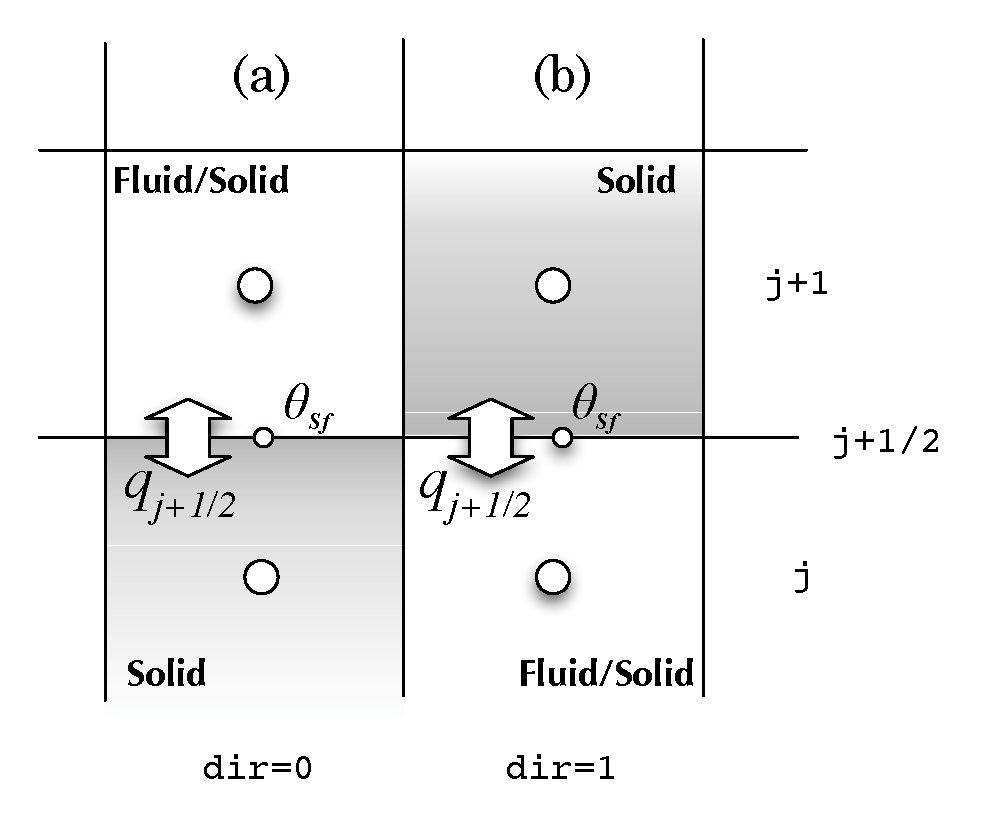
\includegraphics[width=7cm,clip]{Isothermal.eps}
\caption{等温境界のパターン.方向フラグdirはIsoThermalセルの位置と法線方向を示す.}
\label{fig:iso-thermal}
\end{center}
\end{figure}

\noindent \textbf{図\ref{fig:iso-thermal}}において,色塗りのSolidセルは IsoThermalのIDがつけられたセルである.(a), (b) の各パターンはIsoThermalセルの位置が異なる.dir は前処理段階で設定される方向インデクスである.(a) の場合は,界面と温度指定のSolidセルのインデクスが両方とも j であるので,dir=0 とする.このとき,IsoThermalセルからの法線方向は正である.一方,(b) の場合は,界面インデクスはjであるが,等温指定のSolidセルは j+1 なので,dir=1 とする.このとき,IsoThermalセルからの法線方向は負である.

(a)のパターン(dir=0)を考える.セル j は固体セルで,表面温度は常に指定温度である.計算する方のセル j+1 側からの熱流束を考えると,片側近似により,

\begin{equation}
{{q}'}_{{ISO}{\mathrm{,}}\hspace{0.33em}{j}\mathrm{{+}}{1}{\mathrm{/}}{2}}\mathrm{{=}}\mathrm{{-}}{{\mathit{\lambda}}}_{{j}\mathrm{{+}}{1}}\frac{{{\mathit{\theta}}'}_{{j}\mathrm{{+}}{1}}\mathrm{{-}}{{\mathit{\theta}}'}_{sf}}{{{h}'}\slash{2}}
\label{eq:qiso1}
\end{equation}

\noindent 無次元化すると,

\begin{equation}
q_{ISO,\hspace{0.3em}j+1/2} 
\sim
\frac{q_{ISO}^{\prime}}{u_{\mathit{0}}^{\prime} \Delta \theta^{\prime}} \frac{1}{\rho^{\prime}C}
\,=\,
- \frac{1}{u_{\mathit{0}}^{\prime} \Delta \theta^{\prime}} \frac{\lambda_{j+1}}{\rho^{\prime}C}\frac{\theta_{j+1}^{\prime} - \theta_{sf}^{\prime}}{h^{\prime}\slash{2}}
\,=\,
- \frac{2}{u_{\mathit{0}}^{\prime} L^{\prime}} \frac{\lambda_{j+1}}{\rho^{\prime}C} \frac{\theta_{j+1} - \theta_{sf}}{h}
\label{eq:qiso2-1}
\end{equation}

一方,(b)のパターン(dir=1)は,セル j+1 は固体セルで常に指定温度である.

\begin{equation}
{{q}'}_{{ISO}{\mathrm{,}}\hspace{0.33em}{j}\mathrm{{+}}{1}{\mathrm{/}}{2}}\mathrm{{=}}\mathrm{{-}}{{\mathit{\lambda}}}_{j}\frac{{{\mathit{\theta}}'}_{sf}\mathrm{{-}}{{\mathit{\theta}}'}_{j}}{{{h}'}\slash{2}}
\label{eq:qiso2}
\end{equation}

\begin{equation}
q_{ISO,\hspace{0.3em}j+1/2} 
\sim
\frac{q_{ISO}^{\prime}}{u_{\mathit{0}}^{\prime} \Delta \theta^{\prime}} \frac{1}{\rho^{\prime}C}
\,=\,
- \frac{1}{u_{\mathit{0}}^{\prime} \Delta \theta^{\prime}} \frac{\lambda_{j}}{\rho^{\prime}C}\frac{\theta_{sf}^{\prime} - \theta_{j}^{\prime}}{h^{\prime}\slash{2}}
\,=\, - \frac{2}{u_{\mathit{0}}^{\prime} L^{\prime}} \frac{\lambda_{j}}{\rho^{\prime}C}\frac{\theta_{sf} -\theta_{j}}{h}
\label{eq:qiso3}
\end{equation}

\noindent 計算する流体または固体セルは$j+1-dir$で表されること,基準セルに注意してパターン(a), (b) をまとめると,単媒質の場合,

\begin{equation}
q_{ISO,\hspace{0.3em}j+1/2} 
\,=\,
- \frac{2}{u_{\mathit{0}}^{\prime} L^{\prime}} \frac{\lambda_{j+1-dir}}{\rho^{\prime}C}\frac{\theta_{j+1-dir}-\theta_{sf}}{h} \left( 1-2dir \right)
\label{eq:qiso4}
\end{equation}

\noindent ここで$1-2dir$はパターン(a)のとき,つまり$dir=0$のときに法線が正になるように構成している.\\

次の例では,ID=70とID=1に挟まれる面を30度の等温面として扱うことを指定している.

\begin{indentation}{3zw}{0zw}
{
\small
\begin{program}
<Elem name="Iso_Thermal" id="70"  comment="iso_1">
  <Param name="def_face"    dtype="INT"    value="1" />
  <Param name="Temperature" dtype="REAL" value="30.0"/>
</Elem>
\end{program}
}
\end{indentation}

%
\subsubsection{輻射境界 $q_R$}
熱輻射の計算を行う場合に用いる.輻射境界条件は,形態係数の計算を行い輻射流束の収支計算を行った後,その熱流束を直接熱流束境界として与える.

\begin{indentation}{3zw}{0zw}
{
\small
\begin{program}
<Elem name="Heat_Face" id="0">
  <Elem name="Radiation" id="75"  comment="rad_1">
    <Param name="def_face"    dtype="INT"    value="1" />
    <Param name="epsilon" dtype="REAL" value="0.2"/>
    <Param name="projection" dtype="REAL" value="0.6"/>
  </Elem>
</Elem>
\end{program}
}
\end{indentation}

%
\subsubsection{断熱境界 $q_A$}
断熱境界$q_A$は空間におけるセル数の出現頻度が多くなることが予想されるため,他の境界条件とは異なり,断熱マスクにより離散式中に組み込んでいる.このため,モデル作成時にIDで指定することになる.
断熱面の境界条件は,Adiabatic の指定により導入する.
Adiabaticの指定は,idとdef\_faceで指定される面を断熱境界と解釈する.下記の例では,ID=40とID=1で挟まれる面が断熱面となる.

{
\small
\begin{program}
<Elem name="Adiabatic" id="40" comment="insulation">
  <Param name="def_face"    dtype="INT"    value="1" />
</Elem>
\end{program}
}

\begin{figure}[htdp]
\begin{center}
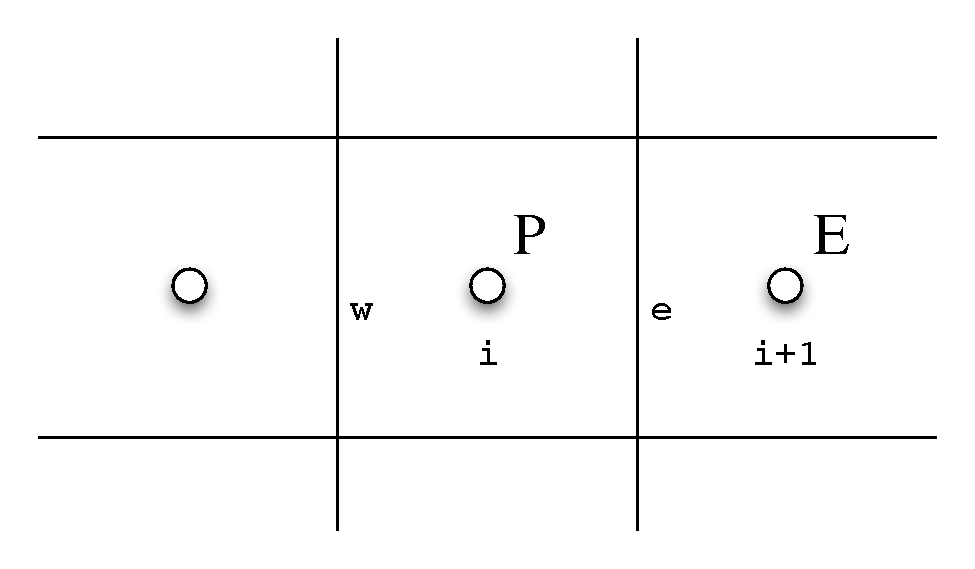
\includegraphics[width=7cm,clip]{AdiabaticBC.eps}
\caption{セルインデックスとセル界面の指定}
\label{fig:face definition}
\end{center}
\end{figure}

\textbf{図\ref{fig:face definition}}において,$e$面($i+1/2$ 位置のセル面)が断熱面の場合,断熱フラグはセル要素に対してスタガード変数配置と同じインデクスで表す.今,$i$ 方向の $e$ 面が断熱面とすると,\textbf{図\ref{fig:BCIndex}}のBC Index の18ビット目を0にして,BCの情報をエンコードする.
断熱条件は,断熱マスク式(\ref{eq:gamma A definition})により実装される.


%
\subsection{セルボリュームに対する熱境界条件の実装}
\label{sec:volume heat bc}
%
\subsubsection{発熱源}
発熱・吸熱の境界条件は,セルボリュームに対して与える.単位体積あたりの発熱量$Q^\prime \,[W/m^3]$が与えられると,発熱項は\textbf{式(\ref{eq:passive scalar1-2 ND})}により無次元化される.ボクセルモデルのIDに対して,XMLファイルで熱源を発熱量(heat release value)または発熱密度(heat generation density)により指定する.この例では,ID=246 に対して,10.0 $[W/m^3]$ の発熱密度を与えている.
{
\small
\begin{program}
<Elem name="Heat_Volume" id="1">
  <Elem name="Heat_Generation" id="246" comment="Desktop">
    <Param name="heat_generation_density" dtype="REAL" value="10.0"/>
  </Elem>
</Elem>
\end{program}
}

熱源項は,安定性のため一時刻前の値を用いて線形化する.ここで注意すべき点は,発熱源の媒質の物性値の指定である(\textbf{式(\ref{eq:qV2})}中の$\rho^{\prime},\,C$)).単媒質の場合には,指定された媒質の物性値を用いる.現物が複数の媒質から構成されている場合には適切な物性値を推定する必要がある.

\begin{equation}
{\mathit{\theta}}^{\hspace{0.15em}n+1}\,=\,{\mathit{\theta}}^{\hspace{0.15em}n}\,+\,\Delta t\,RHS\,+\,\mathrm{\Delta}{t}\,{\mathrm{\Theta}}_{V}^{\hspace{0.15em}n}{\mathrm{,}}
\qquad
{\mathrm{\Theta}}_{V}^{\hspace{0.15em}n}\,=\,\frac{{Q^{\prime}}^{n}}{{\mathit{\rho}}'C}\frac{L^{\prime}}{{u_{\mathit{0}}}^{\prime}\Delta \theta^{\prime}}
\label{eq:qV2}
\end{equation}

%
\subsubsection{定温熱源}
温度を指定する場合には,強制的に指定セルの温度を与える.
{
\small
\begin{program}
<Elem name="Heat_Volume" id="1">
  <Elem name="Const_Temperature" id="247" comment="Tape">
    <Param name="temperature" dtype="REAL" value="45.0"/>
  </Elem>
</Elem>
\end{program}
}

%1ステップの温度を計算後に境界条件で上書きする方法と,Active\_Bitを利用して最初に1回温度を与えるだけで,毎回の境界条件処理を省く方法.時間的に変化する温度を与える場合には毎回処理する.

%
\subsubsection{熱交換器モデル}
\begin{comment}
流体部品として,熱交換器とファンを考える.熱交換器は,圧力損失を生じる多孔質物体で流出方向が法線で与えられる.圧力損失は通過流量(流速)と圧力損失量の関係式が与えられるものとする.一方,ファンも圧力利得が,やはり関係式として与えられる.ファンの場合には旋回成分などもあるが,ここでは軸流方向のみを考える.

流体部品のモデル指定は,セルボリュームに対する内部境界条件として指定する.
\end{comment}


%
\section{多媒質の熱流動現象}
多媒質の熱流動現象とは,文字通り,複数の媒質にわたる熱流動現象である.流体のみに限ると,多相流や多成分流などがこの範疇に入る.同時に,固体熱伝導現象における多媒質間の熱移動も含む.

%
\subsection{固体熱伝導と流体の熱移動現象のスケーリング}
水とアルミニウムの場合の熱移動現象を考える.水のバルクにおける拡散係数を系の代表的な量と考える.\textbf{表\ref{tbl:medium property}}の熱拡散係数の値から,水とアルミニウムの熱拡散速度の比は,$0.143/96.8=1.47\times10^{-3}$ である.つまり,水の熱拡散速度はアルミニウムの$10^{-3}$倍になり,熱の伝わり方が非常に遅い.この時間スケールが大きく異なる点は計算効率の上で大きな問題点である.一方,鉄と空気の場合には,熱拡散の速度は同じオーダであるので,流動側の代表速度でスケーリングしても問題ない.

\begin{table}[htdp]
\caption{物性値の例}
\begin{center}
\small
\begin{tabular}{lcccc}\toprule
 & $\lambda$ & $\rho$ & $C$ & $\alpha$\\ 
 & $[W/(mK)]$ & $[kg/m^3]$ & $[J/(kgK)]$ & $\times 10^{-6}\, [m^{2}/s]$\\ \midrule
Air & $25.7 \times 10^{-3}$ & 1.2 & 1007 & 21.2\\
Water & $598 \times 10^{-3}$ & 998.2 & 4182 & 0.143\\
Fe & 80.3 & 7870.0 & 442 & 22.7\\
Al & 237.0 & 2688.0 & 905 & 96.8\\ \bottomrule
\end{tabular}
\end{center}
\label{tbl:medium property}
\end{table}


固体と流動の熱移動現象を同時に扱う共役熱移動問題を解く場合,対象とする現象によって,以下の2つのアプローチが考えられる.

\begin{itemize}
\item 流体と固体の方程式に対して同じスケーリングを行い,場を統一的に解く.時間進行に関して境界部での熱流束の計算は正確にできるので,非定常現象を扱うことができる.この場合,現象の時定数が異なると非効率になる.
\item 流体と固体側でスケーリングを個別に行い,それぞれ別の方程式を境界で整合する熱流束を授受しながら解き進める.時間スケールが異なることに起因して,合理的な熱流束の授受(境界条件)が必要となる.
\end{itemize}

対象とする作動流体と固体の物性値と流速によっては,時間スケールの違いから非効率な計算となることがある.そこで,始めに流体の時間スケールで解く方法,その後個別の時間スケールで解く解法について述べる.

%
\subsubsection{多媒質の場合の支配方程式}
本来は,保存量であるエネルギーを基本変数にした保存系の方程式を解けばよいが,非圧縮領域では分離解法の方が低コストであること,種々のモデリング手法が適用しやすいことから非圧縮近似による非保存のパッシブスカラ方程式を解く.単媒質の場合と同様に,有次元での計算は有効桁数の制約から桁落ちなどの問題が生じるため,$\theta \sim \mathrm{O}(1)$となるようにできるだけ無次元化して解きたい.
支配方程式は\textbf{式(\ref{eq:passive scalar1 ND})}であるが,多媒質中における輸送現象は物性値が局所的に異なるため,単媒質の場合の\textbf{式(\ref{eq:NS eq:ND})}のように単純な形式での無次元化は難しい.
そこで,物理熱流束の保存性,離散化時の界面での連続性に注意する.拡散項に対して,多媒質では単一のペクレ数を導入した\textbf{式(\ref{eq:passive scalar1 ND})}のような無次元化ができない.したがって,離散化時の桁落ちなどの点を考慮して,半無次元的な実装を行う.\textbf{式(\ref{eq:passive scalar eq})}から,

\begin{equation}
\frac{\partial \theta}{\partial t} \,+\, \frac{\partial}{\partial {x_{i}}} \left({ {{u}_{i}} \theta }\right)
\, =\,
\frac{1}{\rho^{\prime}C} \left[{ \frac{\partial}{\partial{x_{i}}} \left({ \lambda \frac{\partial\theta}{\partial{x_{i}}} }\right) }\right] \frac{1}{{u_{\mathit{0}}}^{\prime} L^{\prime}} \,+\, \Theta_{V}
\label{eq:mm scalar ND}
\end{equation}

\textbf{式(\ref{eq:mm scalar ND})}は拡散項の計算に物理熱流束の温度勾配のみを無次元化した半無次元的な熱流束を用いている.この半無次元熱流束は,物理熱流束とは$1/(u_{0}^{\prime}L^{\prime})$の定数倍だけ異なるが,セル界面で連続である.拡散項の係数$1/({\rho}^{\prime}C)$はセル中心の温度と結びつく熱容量であるので熱流束の計算とは定義点が別であることに注意する.拡散項は次節のモデリングに従う.

%
\subsubsection{拡散項のモデリング}
バイナリボクセルを用いて熱伝導を解く場合,物体境界がセル界面に位置していない場合,あるいは,異なる熱伝導率をもつ媒質界面における熱流束の評価が問題となる.対処法として,熱流束を調和平均で表す方法を用いる\cite{pat:80}.\textbf{図\ref{fig:diffusive flux}}において,セル内で物性値は一定とする.セル P と E の間の界面は,中点$e$ではなく$e^*$の場合を考える.セル界面$e^*$における熱流束$q^{\prime}_{e^*}$は,

\begin{equation}
q_{e^{*}}^{\prime} \,=\, q_{e^{+}}^{\prime} \,=\, q_{e^{-}}^{\prime} 
\label{difuusive flux at interface:1}
\end{equation}

\begin{equation}
\left\{{\begin{array}{l}
{{{q}'}_{{e}\mathrm{{+}}}\,=\,\mathrm{{-}}{{\mathit{\lambda}}_{E}}{\mathrm{(}}{{\mathit{\theta}}'}_{E}\mathrm{{-}}{{\mathit{\theta}}'}_{e\mathrm{*}}{\mathrm{)/}}\mathrm{\Delta}{{x}'}_{{e}\mathrm{{+}}}}\\
{{{q}'}_{{e}\mathrm{{-}}}\,=\,\mathrm{{-}}{{\mathit{\lambda}}_{P}}{\mathrm{(}}{{\mathit{\theta}}'}_{e\mathrm{*}}\mathrm{{-}}{{\mathit{\theta}}'}_{P}{\mathrm{)/}}\mathrm{\Delta}{{x}'}_{{e}\mathrm{{-}}}}\end{array}}\right.
\label{eq:difuusive flux at interface:2}
\end{equation}

\begin{figure}[htdp]
\begin{center}
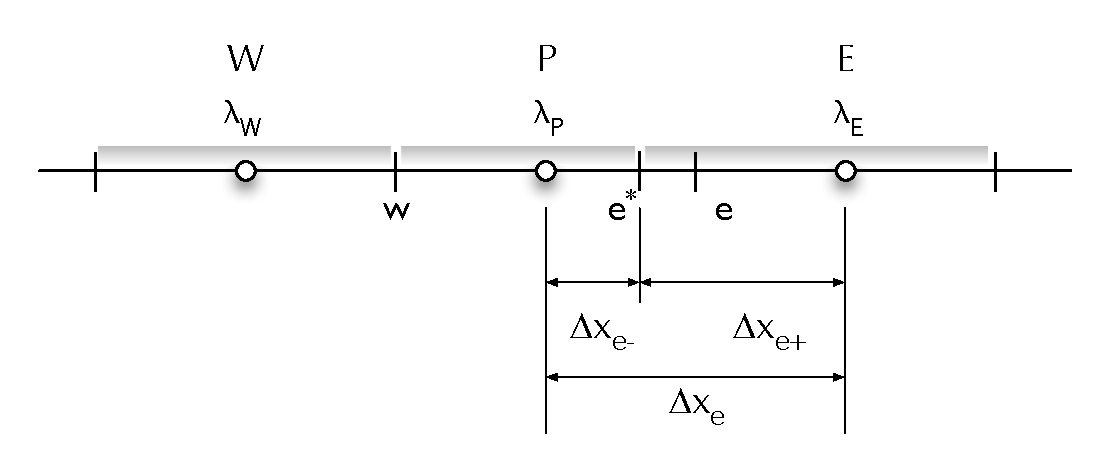
\includegraphics[width=12cm,clip]{face.eps}
\caption{調和平均を用いた拡散項の近似}
\label{fig:diffusive flux}
\end{center}
\end{figure}


これより,熱流束と界面温度は以下のようになる.

\begin{equation}
{{q}'}_{e\mathrm{*}}\,=\,\mathrm{{-}}{\left({\frac{\mathrm{\Delta}{{x}'}_{{e}\mathrm{{+}}}}{{{\mathit{\lambda}}_{E}}}\mathrm{{+}}\frac{\mathrm{\Delta}{{x}'}_{{e}\mathrm{{-}}}}{{{\mathit{\lambda}}_{P}}}}\right)}^{\mathrm{{-}}{1}}\left({{{\mathit{\theta}}'}_{E}\mathrm{{-}}{{\mathit{\theta}}'}_{P}}\right)
\label{eq:difuusive flux at interface:3}
\end{equation}

\begin{equation}
{{\mathit{\theta}}'}_{e\mathrm{*}}\,=\,\frac{{{\mathrm{\varphi}}_{E}}'{{\mathit{\theta}}'}_{E}\mathrm{{+}}{{\mathrm{\varphi}}_{P}}'{{\mathit{\theta}}'}_{P}}{{{\mathrm{\varphi}}_{E}}'\mathrm{{+}}{{\mathrm{\varphi}}_{P}}'}
\label{eq:difuusive flux at interface:4}
\end{equation}

ただし,${\varphi}_{E}^{\prime}\,=\,{\lambda}_{E}/{\Delta x}_{e^{+}}^{\prime},\quad{\varphi}_{P}^{\prime}\,=\,{\lambda}_{P}/{\Delta x}_{e^{-}}^{\prime}$である.

ここで,セル界面が中点$e$の場合を考えてみると,$h^{\prime}$をボクセル幅として,

\begin{equation}
\mathrm{\Delta}{{x}'}_{{e}\mathrm{{+}}}\,=\,\mathrm{\Delta}{{x}'}_{{e}\mathrm{{-}}}\,=\,{h}'/2
\label{eq:difuusive flux at interface:5}
\end{equation}

\begin{equation}
{{q}'}_{e\mathrm{*}}\,=\,\mathrm{{-}}{2}{\left({\frac{1}{{{\mathit{\lambda}}_{E}}}\mathrm{{+}}\frac{1}{{{\mathit{\lambda}}_{P}}}}\right)}^{\mathrm{{-}}{1}}\frac{{{\mathit{\theta}}'}_{E}\mathrm{{-}}{{\mathit{\theta}}'}_{P}}{{h}'}
\label{eq:difuusive flux at interface:6}
\end{equation}

これは,均質媒質のとき拡散流束の標準的な差分近似と同じである.さらに$\lambda_{E}\, \gg \, \lambda_{P}$の場合は$\lambda_{E}$の値が大きいので,\textbf{式(\ref{eq:difuusive flux at interface:6})}は

\begin{equation}
{{q}'}_{e\mathrm{*}}\,=\,\mathrm{{-}}{{\mathit{\lambda}}_{P}}\frac{{{\mathit{\theta}}'}_{E}\mathrm{{-}}{{\mathit{\theta}}'}_{P}}{{{h}'}\slash{2}}
\label{eq:difuusive flux at interface:7}
\end{equation}

となる.\textbf{式(\ref{eq:difuusive flux at interface:7})}は,界面$e^{*}$付近でセル E の温度を$\theta_{E}$と近似した上で片側差分により勾配を近似したことを表している.界面での熱伝導率として調和平均を用いる点に注意する.

\begin{equation}
{{\mathit{\lambda}}_{e\mathrm{*}}} \,=\, {2}\frac{{{\mathit{\lambda}}_{E}}{{\mathit{\lambda}}_{P}}}{{{\mathit{\lambda}}_{E}}\mathrm{{+}}{{\mathit{\lambda}}_{P}}}
\label{eq:difuusive flux at interface:8}
\end{equation}

この方法により,熱拡散係数が異なる媒質間の熱移動を合理的な近似により表現する.

多媒質の場合は,

\begin{equation}
\frac{\theta^{n+1} - \theta^{n}} {\Delta t}
\,=\,
\frac{1}{\rho^{\prime}C} \left[{
\frac{1}{h^{2}} \left\{{
\sum\limits_{j=1}^{\dim\times2} {\left({
\gamma \lambda
}\right)}_{j} \hspace{0.15em}
\theta_{J} \hspace{0.15em}-\hspace{0.15em} \theta_{P} \sum\limits_{j=1}^{\dim\times2}
{\left({
\gamma \lambda
}\right)}_{j}
}\right\}
}\right]
\frac{1}{{u_{\mathit{0}}}^{\prime} L^{\prime}}
\,-\,
\frac{1}{\rho^{\prime}C} \left[{
\frac{1}{h} \sum\limits_{j=1}^{\dim\times2} {
\left({ {-1} }\right)}^{j} \hspace{0.15em}
{\left\{{ 
\left({ {1} - \gamma }\right) q_{BC}^{\prime} 
}\right\}}_{j} 
}\right]
\frac{1}{{u_{\mathit{0}}}^{\prime} \Delta \theta^{\prime}} \,+\, \Theta_{V}
\label{eq:pscalar semi-discrete9}
\end{equation}


%TypeS MM用
ここで$\rho^{\prime}C$は解くべきセルの物性値なので,前処理時に方向インデクスを保存しておく.
境界面を挟む2つのセルのうちどちらが固体要素であるかは,前処理でそのインデクスを特定している.熱伝達境界面をもつインデクスの小さい方のセル(つまり\textbf{図\ref{fig:typeN}}の (a), (b)の両方のパターンともセルj)に熱伝達境界の attribute ID を保持するようにしている.

\textbf{図\ref{fig:typeN}}において,熱境界条件を昇順にサーチし,まずインデクス j を得る.この場合,j+1/2 面が熱伝達形式の境界流束となるので,インデクス j に対して j または j+1 のどちらかが参照側の固体となる.(a) の場合,j 要素が固体なので,j を基準として固体要素の方向を示す値 dir=0 となる.一方 (b) の場合,固体要素は j+1 なので j から見ると,dir=1 である.

多媒質(Multi-Medium, MM)の場合には,セル(i, j)に対する固体要素の参照は (i, j+dir) のように参照できる.一方,流体が単媒質(Single-Medium, SM)の場合には,熱伝達境界条件として与える部分の固体の物性に依存するのみであり,この情報はコンポーネントテーブルから読み取る.


%
\chapter{ドライバ}
{\begin{abstract}
本章では,発達したチャネル流などの解析を実施する際に用いられるドライバ部分の実装について説明する.
\end{abstract}
\graphicspath{{./fig_Driver/}}
%

%
\section{ドライバセクション}
ドライバセクションは,乱流計算などで発達した管路内の流れを流入条件として与える場合に用いられる.
\textbf{図\ref{fig:Driver}}に想定する利用形態を示す.
図では左側から流れが流入し,ドライバセクションで発達流を形成し,内部領域での計算結果を評価する.
流れを有限の領域で発達させるために,ドライバセクションで周期境界を適用し,発達した流れを下流の内部領域に支配方程式を満たしながら接続することを考える.

\begin{figure}[htbp]
\begin{center}
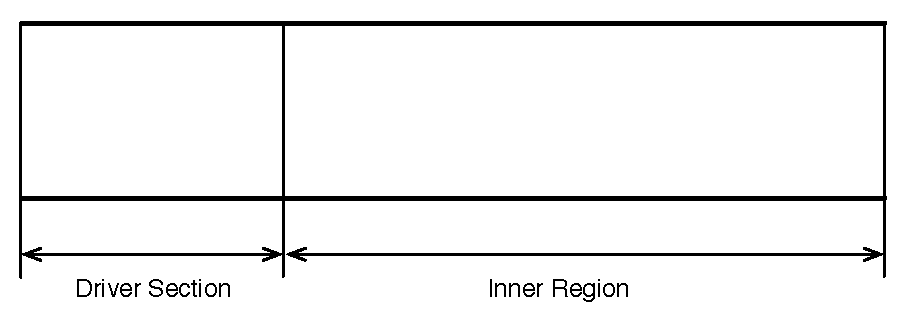
\includegraphics[width=9cm,clip]{Driver.eps}
\end{center}
\caption{ドライバセクションを含む流れ解析.}
\label{fig:Driver}
\end{figure}

%
\subsection{ドライバセクションにおける周期境界の実装}

\textbf{図\ref{fig:Driver_prdc}}にドライバセクションの取り扱いを示す.
ドライバセクションはインデクス\verb|i=1~ip|の領域で,流出部のインデクスが\verb|i=ip|である.
ドライバセクションの目的は,発達した流れを形成し,計算する内部領域へと導くことである.
その際に支配方程式を満たすことが重要となる.

外部境界に対する周期境界であれば,単に,ドライバセクションの前後で計算した物理量を相互に交換すればよい.
ここで注意すべき点は,セル\verb|ip,ip+1|は計算内点にあり,数値流束$f_{ip+1/2}$をドライバセクションと内部領域で一致させる必要があることである.
単にデータを交換することは難しく,例えば一旦物理量を待避させ,その間に周期処理を行い,その後待避した物理量を戻すという処理などが必要になる.
つまり,特殊な操作をしないと通常のステンシル型の計算スキームでは境界条件を実装しにくい.
この点は,処理の複雑さによる処理コストの増加と並列計算時には同期待ちを生じるため,演算性能の低下につながる.

\begin{figure}[htbp]
\begin{center}
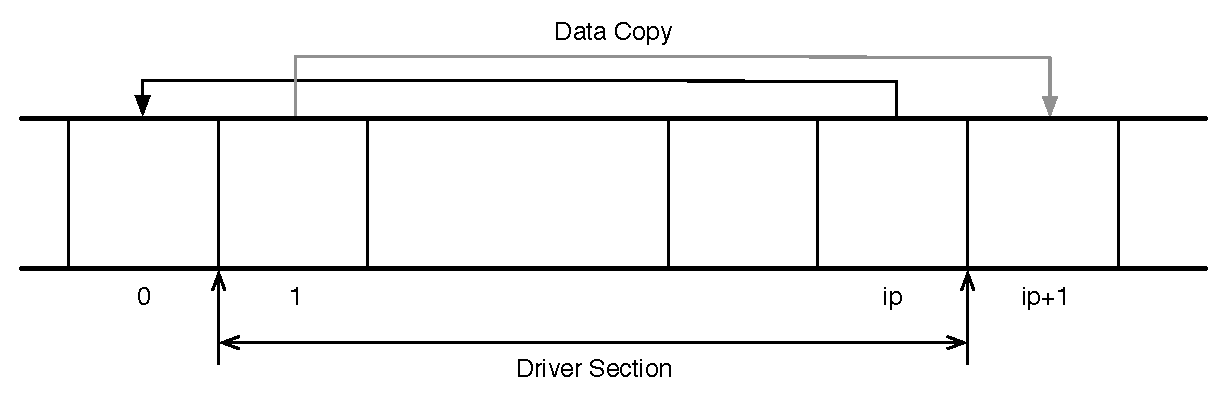
\includegraphics[width=13cm,clip]{Driver_prdc.eps}
\end{center}
\caption{ドライバセクションにおける周期境界処理.}
\label{fig:Driver_prdc}
\end{figure}

そこで,本来の目的に立ち返り,完全な周期境界でなく,あくまで流れを発達させることに重点をおき,なおかつ処理コストが低い方法を考える.
実装する方法は,以下のようになる.
\begin{itemize}
\item ドライバセクションでは,計算領域内部に用いる部分的な周期境界条件を実装する.
\item ドライバセクションの形状的な条件として,流入部と流出部の断面形状は同一で,座標軸に対して面直であること.必ず計算空間を構成する6面のどれかに接続していること.ドライバセクションは複数あっても良い.
\item 周期条件は,流出面から流入面へのone wayとする.計算は,ドライバセクションと内部領域にわたり,同じスキームにより計算する.このため,セル界面における数値流束は保存する.このとき,流入面へとコピーされる物理量は下流領域の影響を受けた値となるが,支配方程式を満たした値であるので,これを流入側に与えても問題はない.
\item ドライバセクションは圧力駆動とする.つまり,ドライバセクションの両端に圧力差を与え,速度はフリーとする\footnote{このため,計算内部領域の背圧によって流量が変化する可能性もある.その場合には,フィードバック機構を組み込み流量調整をする必要がある.}.
\end{itemize}

\subsubsection{速度}
速度の場合は,利用する空間スキームのステンシルに応じてデータをコピーする.

\subsubsection{圧力}
圧力の場合は,与える圧力差を$p_d$として,次式のように圧力値をコピーする.
\begin{equation}
p_0 \,=\, p_{ip} + p_d
\end{equation}

\subsubsection{パッシブスカラ}
非圧縮の温度のようなパッシブスカラ値については,ドライバセクション流出部の状況によらず,常に流入部で指定値を与える.


%
\subsection{ボクセルモデルの指定}
\textbf{図\ref{fig:Driver_voxel}}にドライバセクションを指定する場合のボクセルIDの例を示す.ドライバセクションの内部とは別のIDで出口断面を与える点に注意する.

\begin{figure}[htbp]
\begin{minipage}{.65\textwidth}
\begin{center}
\includegraphics[width=10cm,clip]{Driver_voxel.eps}
\end{center}
\end{minipage} \hfill
\begin{minipage}{.3\textwidth}
\begin{center}
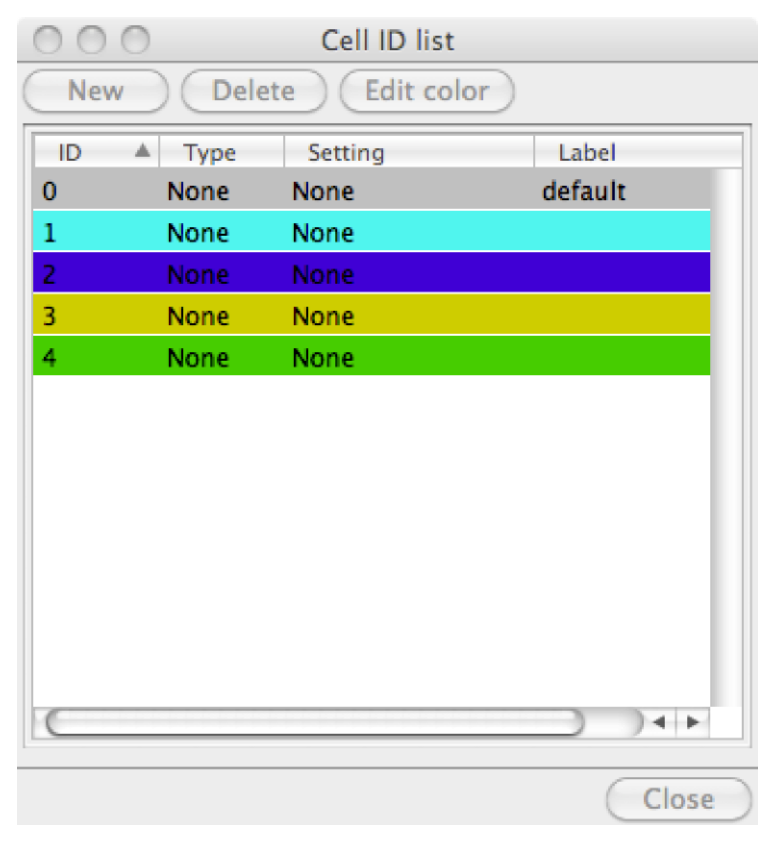
\includegraphics[width=5cm,clip]{Cell_id.eps}
\end{center}
\end{minipage}
\caption{チャネル流のボクセル設定.ID=1:内部流体,ID=2:固体セル,ID=3:ドライバセクション(流体),ID=4:ドライバセクションの流出断面(流体).}
\label{fig:Driver_voxel}
\end{figure}

%
\pagebreak
\subsection{境界の指定方法}
\textbf{図\ref{fig:Driver_voxel}}を例に,境界条件の指定方法を示す.
ドライバセクションを利用するためには,内部境界と外部境界の両方の指定が必要になる.

\subsubsection{内部境界}
{ \small
\begin{program}
<InnerBoundary>
  <Elem comment="inner_driver" id="4" name="Periodic">
    <Param dtype="STRING" name="Upstream_Direction"  value="X_minus"/>
    <Param dtype="REAL"   name="Pressure_Difference" value="1.636e-4"/>
    <Param name="def_face"  dtype="INT"  value="1" />
  </Elem>
</InnerBoundary>
\end{program}
}

内部境界で指定するUpstream\_Directionと外部境界で指定するDriver\_Directionの方向は同じであること.

\subsubsection{外部境界}

{ \small
\begin{program}
<OuterBoundary>
  <Elem id="10" name="Periodic">
    <Param dtype="STRING" name="Mode" value="Driver"/>
    <Param dtype="STRING" name="Driver_Direction" value="X_minus"/>
    <Param dtype="int"    name="Driver_Lid_Index" value="28"/>
  </Elem>
</OuterBoundary>
\end{program}
}

Driver\_Lid\_Indexには,流入方向の空間インデクス値を指定する.
この値がわからない場合には,適当な値をいれておき,CBCソルバを実行すると,コンポーネント情報の部分に下記のように表示されるので,その値を入力する.この例の場合には,X\_Minus方向がドライバの方向なので,i\_stの値を入力する.

{ \small
\begin{program}
>> Component Information

[Periodic]
 no            Label  ID  i_st  i_ed  j_st  j_ed  k_st  k_ed  Pressure Difference [Pa]/[-]  Driver
  1     inner_driver   4    28    28     2    29     2    29     1.63600e-04 / 3.21221e-01      X-
\end{program}
}



%
\chapter{物理量のモニタリングクラス}
{\begin{abstract}
本章では,計算中の任意点の物理量をモニターする仕組みについて解説する.
\end{abstract}
\graphicspath{{./fig_Sample/}}


物理量モニタリング機能は,ユーザが指定した位置で指定した物理量をファイルに出力する機能である.
位置の指定には,ボクセルモデルのIDで指定する方法とXMLパラメータファイルで指定する2種類がある.
ここでは内部実装について説明する.

%%%
\section{物理量モニタリング機能API}
物理量モニタリング機能は,全モニタグループを管理するMonitorListクラス,
個々のモニターグループを管理するMonitorCompoクラス,
各モニタ点でのサンプリング機能を提供するSamplingクラスより構成される.

\begin{figure}[H]
\vspace{0.5cm}
\begin{center}
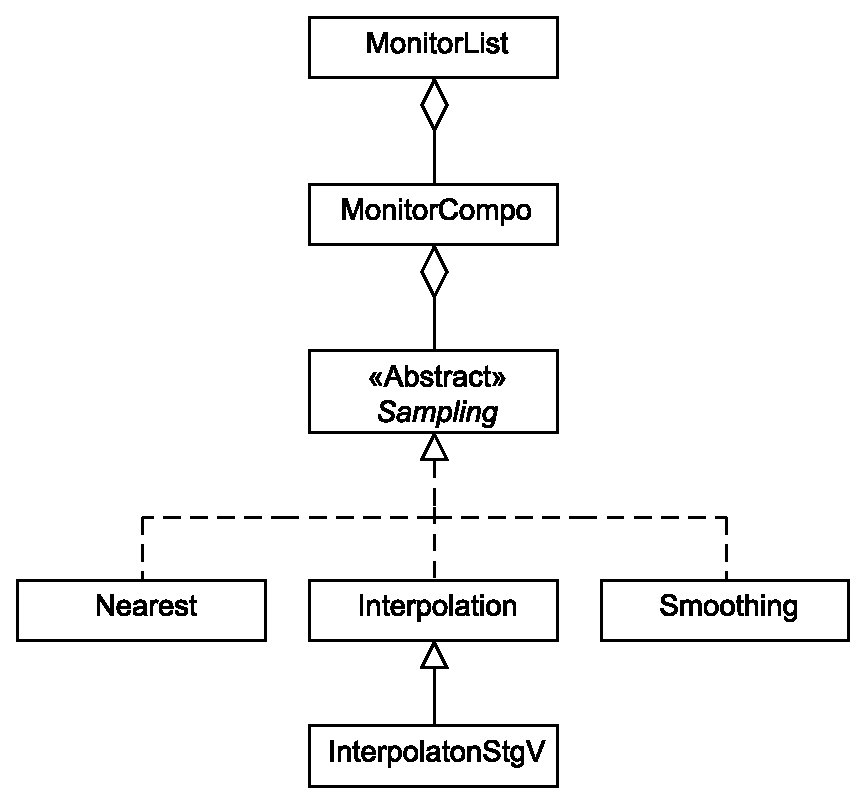
\includegraphics[width=0.7\textwidth]{Monitor.eps}
\caption{物理量モニタリング機能のクラス図}
\label{fig:monitor}
\end{center}
\end{figure}

MonitorListクラスおよびMonitorCompoクラスは,Parallel\_Nodeクラスを継承している.
Samplingクラスは抽象クラスで,
各モニタ点での実際のサンプリング計算は,Samplingクラスから継承された
Nearestクラス,Interpolationクラス,Smoothingクラスが担当する.
ソルバーから直接インスタンスされ操作されるのは,MonitorListクラスのみである.

\pagebreak
%%%
\subsection{MonitorListクラス公開メソッド}
%
\vspace{2mm}

\paragraph{必須パラメータのコピー}\mbox{}\\
モニタリング機能の管理およびサンプリング計算に必要なパラメータをコピーする.

\begin{table}[hp]
\begin{tabular}{ll}
{\tt bcd} & BCindex ID配列\\
{\tt g\_org} & グローバル領域基点座標\\
{\tt g\_lbx} & 領域サイズ\\
{\tt org} & ローカル領域基点座標\\
{\tt dx} & セル幅\\
{\tt lbx} & 領域サイズ\\
{\tt rs} & ローカルセルサイズ\\
{\tt gc} & ガイドセル数\\
{\tt refVelocity} & 代表速度\\
{\tt baseTemp} & 基準温度\\
{\tt diffTemp} & 代表温度差\\
{\tt refDensity} & 代表密度\\
{\tt refLength} & 代表長さ\\
{\tt basePrs} & 基準圧力\\
{\tt modeUnit} & 出力単位の指定フラグ(有次元,無次元)\\
{\tt unitTemp} & 温度の単位\\
{\tt modePrecision} & 精度のフラグ(単精度,倍精度)\\
{\tt unitPrs} & 圧力の単位\\
{\tt v00} & 座標系移動速度と成分\\
\end{tabular}
\end{table}

{\small
\begin{program}
void setControlVars(unsigned* bcd, SKL_REAL g_org[3], SKL_REAL g_lbx[3],
                  SKL_REAL org[3], SKL_REAL dx[3], SKL_REAL lbx[3],
                  unsigned rs[3], unsigned gc,
                  SKL_REAL refVelocity, SKL_REAL baseTemp, SKL_REAL diffTemp,
                  SKL_REAL refDensity, SKL_REAL refLength, SKL_REAL basePrs,
                  unsigned modeUnit, unsigned unitTemp,
                  unsigned modePrecision, unsigned unitPrs)
\end{program}
}

%
\paragraph{参照速度の指定}\mbox{}\\
引数{\tt v00[4]}には,参照格子系の速度と速度成分をもつ配列を指定する.
{\small
\begin{program}
void set_V00(SKL_REAL v00[4]) 
\end{program}
}

%
\paragraph{出力タイプの設定}\mbox{}\\
引数{\tt type}には,{\tt MonitorList::GATHER}(単一ファイル出力)
または{\tt MonitorList::DISTRIBUTE}(分散出力)を指定する.
{\small
\begin{program}
void setOutputType(OutputType type)
\end{program}
}

%
\paragraph{point\_setグループの登録}\mbox{}\\
ラベル文字列{\tt labelStr},モニタ対象物理量文字列のvector {\tt variables},
サンプリング方法文字列{\tt methodStr},
サンプリングモード文字列{\tt modeStr},
MonitorPoint構造体のvector {\tt pointSet}によりpoint\_setグループを登録する.
\pagebreak
{\small
\begin{program}
void setPointSet(const char* labelStr, vector<string>& variables,
                 const char* methodStr, const char* modeStr,
                 vector<MonitorCompo::MonitorPoint>& pointSet)
\end{program}
}
MonitorPoint構造体は,個々のモニタ点に対応した構造体である.

{\small
\begin{program}
struct MonitorPoint {
  Vec3r crd;      ///< モニタ点座標
  string label;   ///< モニタ点ラベル(コメント)
  MonitorPoint(const SKL_REAL v[3], const char* str) : crd(v), label(str) {}
  ~MonitorPoint() {}
};
\end{program}
}

%
\paragraph{lineグループの登録}\mbox{}\\
ラベル文字列{\tt labelStr},モニタ対象物理量文字列のvector {\tt variables},
サンプリング方法文字列{\tt methodStr},
サンプリングモード文字列{\tt modeStr},
線分端点座標{\tt from,to},分割数{\tt nDivision}
によりlineグループを登録する.
{\small
\begin{program}
void setLine(const char* labelStr, vector<string>& variables,
             const char* methodStr, const char* modeStr,
             SKL_REAL from[3], SKL_REAL to[3], int nDivision)
\end{program}
}

%
\paragraph{内部境界条件としてのモニタ指定の有無を調査}\mbox{}\\
サイズ{\tt nBC}のコンポーネント配列{\tt cmp}を調べ,
内部境界条件としてのモニタ指定があればtrueを返す.
{\small
\begin{program}
bool hasCellMonitor(CompoList* cmp, int nBC) 
\end{program}
}

%
\paragraph{内部境界条件としてのモニタ領域を登録}\mbox{}\\
サイズ{\tt nBC}のコンポーネント配列{\tt cmp}を参照して,
内部境界条件として指定されたモニタ領域を登録する.
{\small
\begin{program}
void setInnerBoundary(CompoList* cmp, int nBC)
\end{program}
}

%
\paragraph{サンプリング元となるデータ配列の登録}\mbox{}\\
速度変数配列{\tt v},
圧力変数配列{\tt p},
温度変数配列{\tt t}を登録.
{\small
\begin{program}
void setDataPtrs(SKL_REAL* v, SKL_REAL* p, SKL_REAL* t=NULL)
\end{program}
}

%
\paragraph{モニタ点位置情報の出力}\mbox{}\\
セルID配列{\tt id}に対して,
point\_setグループおよびlineグループのモニタ点を含むセルに対して
ID=255を書き込む.
{\small
\begin{program}
void write_ID(int* id)
\end{program}
}

%
\pagebreak
\paragraph{モニタリング情報を出力}\mbox{}\\
ファイルポインタ{\tt fp}に,
登録されたモニタリング設定情報を出力する.
{\small
\begin{program}
void printMonitorInfo(FILE* fp)
\end{program}
}

%
\paragraph{出力ファイルのオープン}\mbox{}\\
文字列{\tt str}にXMLコンフィギュレーションファイルの
OutputData要素のlog\_samplingで指定されたファイル名を渡すことにより,
各グループ用,各ノード用(分散出力時)のファイル名が生成され,オープンされる.
このメソッドは,出力タイプによらず,全プロセスから呼んでも問題ない.
{\small
\begin{program}
void openFile(const char* str)
\end{program}
}

%
\paragraph{サンプリング計算(point\_set, line)}\mbox{}\\
以下のメソッドにより,point\_setグループおよびlineグループの
各モニタ点でサンプリング計算を行う.
{\small
\begin{program}
void sampling()
\end{program}
}

%
\paragraph{サンプリング計算(内部境界条件)}\mbox{}\\
内部境界条件として指定されたモニタ領域のサンプリングには
次のメソッドを用いる.
このメソッドで,サンプリング結果のノード0への集計,モニタ領域内での平均,
速度の場合は法線ベクトルとの内積を計算し,コンポーネントcmpへの格納までを行う.
{\small
\begin{program}
void samplingInnerBoundary()
\end{program}
}

%
\paragraph{サンプリング結果の出力}\mbox{}\\
サンプリング時のステップ数{\tt step}およびソルバー内部時間{\tt tm}
とともに,サンプリング結果をファイルに出力する.
単一ファイル出力の場合も,このメソッド内部で集約計算を行うため,
全プロセスから呼ぶ必要がある.
{\small
\begin{program}
void print(unsigned step, SKL_REAL tm)
\end{program}
}

%
\paragraph{出力ファイルのクローズ}\mbox{}\\
オープンしていた全ての出力ファイルをクローズする.
出力タイプによらず,全プロセスから呼んでも問題ない.
{\small
\begin{program}
void closeFile()
\end{program}
}

%%%
\pagebreak
\section{ソルバーへの組み込み方法}
MonitorListクラスを利用するためには,ヘッダファイルMonitor.hをインクルードする.

\subsection{初期化}
以下の8ステップが必要:

\begin{enumerate}
\item インスタンス化
\item setParallelInfoメソッドによる並列情報の設定
\item setControlVarsメソッドによる必須パラメータのコピー
\item setPointSetメソッド,setLineメソッドによるpoint\_setグループとlineグループの登録(これらの操作は,Control::setMonitorメソッド内で行われる)
\item write\_IDメソッドにより,モニタ点位置のセルIDに255を書き出す
\item setInnerBoundaryメソッドによる内部境界条件指定のモニタ領域の登録
\item openFileメソッドによるモニタ結果出力ファイルのオープン
\item setDataPtrsメソッドによるサンプリング元データ配列の登録
\end{enumerate}

{\small
\begin{program}
  Control       C;
  Parallel_Info pn;
  CompoList*    cmp;
  …
  // (1) インスタンス化
  MonitorList MO;
  …

  // (2) 並列情報設定
  MO.setParallelInfo(pn);

  // (3) 必須パラメータのコピー
  MO.setControlVars(bcd, G_org, G_Lbx, C.org, C.dx, C.Lbx, size, guide,
               C.RefVelocity, C.BaseTemp, C.DiffTemp, C.RefDensity, C.RefLength,
               C.BasePrs, C.Unit.Param, C.Unit.Temp, C.Mode.Precision, C.Unit.Prs);

  // (4) Control::setMonitorメソッドの中で,XMLファイルをパースして,
  //     setPointSetメソッドによりpoint_setグループを,
  //     setLineメソッドによりlineグループを登録している
  C.setMonitor(&MO);

  // (5) モニタ点位置のセルIDに255を書き出す
  MO.write_ID(mid);

  // (6) 内部境界条件指定のモニタ領域の登録
  MO.setInnerBoundary(cmp, C.NoBC);

  // (7) モニタ結果出力ファイルのオープン
  //    (出力タイプによらず全プロセスでopenFileメソッドを呼ぶ)
  MO.openFile(C.HistoryMonitorName);

  // (8) サンプリング元となるデータ配列の登録
  if (C.isHeatProblem()) {
    MO.setDataPtrs(dc_v->GetData(), dc_p->GetData(), dc_t->GetData());
  } else {
    MO.setDataPtrs(dc_v->GetData(), dc_p->GetData());
  }
\end{program}
}

%
\pagebreak
\subsection{サンプリングおよびファイル出力}

非定常計算の場合には,タイムステップループ中に格子の移動速度が変化する場合もあるので,参照速度を各タイムステップ内でモニタークラスに渡す.
{\small
\begin{program}
  // SKL_REAL v00[4] で宣言
  MO.set_V00(v00);
\end{program}
}

point\_setグループおよびlineグループに対するサンプリングには
samplingメソッドを用いる.
サンプリング結果の出力には,全プロセスからprintメソッドを呼ぶ.
{\small
\begin{program}
  // サンプリング
  MO.sampling();

  // ファイル出力
  // (出力タイプによらず全プロセスでprintメソッドを呼ぶ)
  MO.print(m_currentStep, (SKL_REAL)SklGetTotalTime());
\end{program}
}

内部境界条件指定によるモニタ領域のサンプリングには
samplingInnerBoundaryメソッドを用いる.
サンプリング結果の出力は,History::printHistoryCompoメソッドが担当する.
{\small
\begin{program}
  // サンプリング
  MO.samplingInnerBoundary();
  
  // ファイル出力はHistoryクラスが担当
  if (pn.ID == 0) H.printHistoryCompo(fp_c, this, cmp, &C);
\end{program}
}

%
\subsection{サンプリング方法の追加・改良方法}
nearest, interpolation, smoothingの各サンプリング方法は,
抽象クラスSamplingを継承した,Nearestクラス,Interpolationクラス,
Smoothingクラスでそれぞれ実装されている.

サンプリング方法の追加・改良するには,
Samplingクラスを継承した新たなクラスを作成する方法と,
既存の3クラス(Nearest,Interpolation,Smoothing)から継承した新クラスを作成する方法がある.

%
\subsection{Samplingクラスを継承する方法}
Samplingクラスを継承したクラスでは,
次の5つメソッドを実装する必要がある.

{\small
\begin{program}
// 速度をサンプリング
Vec3r samplingVelocity(const SKL_REAL* v);

// 圧力をサンプリング
SKL_REAL samplingPressure(const SKL_REAL* p);

// 温度をサンプリング
SKL_REAL samplingTemperature(const SKL_REAL* t);

// 全圧をサンプリング
SKL_REAL samplingTotalPressure(const SKL_REAL* v, const SKL_REAL* p);

// 渦度をサンプリング
Vec3r samplingVorticity(const SKL_REAL* v);
\end{program}
}

この時,Samplingクラスで定義された以下のprotectedメソッドを利用することができる.
\pagebreak

%
\paragraph{全圧の計算}\mbox{}\\
速度{\tt v},圧力{\tt p}から計算した全圧値を返す.
{\small
\begin{program}
SKL_REAL calcTotalPressure(const Vec3r v, SKL_REAL p)
\end{program}
}

%
\paragraph{渦度の計算}\mbox{}\\
速度変数配列{\tt v}から,セル位置{\tt index}での渦度を計算して返す.
{\small
\begin{program}
Vec3r calcVorticity(const SKL_REAL* v, Vec3i index)
\end{program}
}

%
\paragraph{セルインデックスのシフト}\mbox{}\\
近傍セルのインデックスを求めるための,
セルインデックス{\tt index}を指定方向にシフトさせる
shift1〜shift7の7メソッド,
shift\_xm〜shift\_zpの6メソッドが提供される.
{\small
\begin{program}
/// セルインデックスを(1,0,0)方向にシフト
Vec3i shift1(Vec3i index)
…
…
/// セルインデックスを(1,1,1)方向にシフト
Vec3i shift7(Vec3i index)

/// セルインデックスを-x方向にシフト
Vec3i shift_xm(Vec3i index) 
…
…
/// セルインデックスを+z方向にシフト
Vec3i shift_zp(Vec3i index)
\end{program}
}

%
\paragraph{セルの状態(流体/固体)を調べる}\mbox{}\\
セル{\tt index}が流体ならtrue, 固体ならfalseを返す.
{\small
\begin{program}
bool isFluid(Vec3i index)
\end{program}
}

%
\paragraph{セルでのスカラー値を取得}\mbox{}\\
スカラー配列{\tt s}のセル{\tt index}での値を返す.
{\small
\begin{program}
SKL_REAL getScalar(const SKL_REAL* s, Vec3i index)
\end{program}
}

%
\paragraph{セルでのベクトル値を取得}\mbox{}\\
ベクトル配列{\tt v}のセル{\tt index}での値を返す.
{\small
\begin{program}
Vec3r getVector(const SKL_REAL* v, Vec3i index)
\end{program}
}

%%%
\pagebreak
\subsection{既存クラス(Nearest,Interpolation,Smoothing)を継承する方法}
Nearestクラス,Interpolationクラス,Smoothingクラスのいずれかを継承し,
その一部のメソッドを上書きすることにより,
基底クラスのサンプリング方法を改良することができる.

現バージョンのソースコード(Sampling.h, Sampling.C)には,
既存クラスからの継承のサンプルとして,
InterpolationStgVクラスを収録してある.
InterpolationStgVクラスは,Interpolationクラスを継承して,
スタガード配置の速度変数配列に対応させたものである.


\subsection{端点処理}
線分の端点が計算対象領域境界上にある場合には,
そのモニタ点がガイドセル側に属すると判断されることがあり,
sampling\_mode=fluidと指定したにもかかわらずモニタ点を含むセルが固体セルであるため,警告メッセージ「{\tt  *skip(unexpected solid)*}」が出力されることがある.

この現象を防止するために,lineグループ指定時の線分端点座標を,
常に実際の計算対象領域よりわずかに小さい領域にクリッピングする仕様としている.




%
\chapter{計算性能モニタクラス}
{\begin{abstract}
本章では,性能測定モジュールの機能について説明する.
\end{abstract}
\graphicspath{{./fig_PM/}}
%

\section{計算性能測定機能}
計算性能測定機能は,
ソルバー実行時に,プログラムコード内の測定対象部分の実行時間を測定し,
その統計情報を出力する機能を提供する.

各測定箇所は,整数値キー番号により識別される.
測定箇所はキー番号以外に,次のプロパティを持つ.
\begin{quote}
\begin{description}
\item[ラベル] 統計情報出力時のラベル文字列
\item[測定対象タイプ] 「計算時間」または「通信時間」
\item[排他測定フラグ] 「排他測定」または「非排他測定」
\end{description}
\end{quote}

\paragraph{測定対象タイプ}
測定を終了するstopメソッドには,オプションとして測定区間の「計算量」を
ユーザが自己申告できる機能がある.
測定対象タイプが計算時間の場合には,この申告量を浮動小数点演算量と解釈し,
統計情報出力時に計算速度(FLOPS値)を出力する.
一方,測定対象タイプが通信時間の場合には,申告量をバイト単位の通信量と解釈し,
統計情報出力時に通信速度(Byte/s単位)を出力する.

\paragraph{排他測定と非排他測定}
測定箇所は,排他測定フラグの真偽により,
「排他測定」と「非排他測定」とに分類される.
排他測定は,「(ほぼ)完成されたプログラムの実行時の状況を把握するために,
プログラムコードを排他的な領域に分割し,各領域の実行時間を測定する」
という使用方法を想定している.排他測定では,統計情報出力時に,
「全排他測定箇所の合計実行時間」に対する
「個々の排他測定箇所の実行時間」の割合も出力する.

一方,非排他測定は,プログラムのデバッグあるいはチューニング時に,一時的に
興味のある対象領域の実行時間を把握するのに使用することを想定している.
そのため,非排他測定区間は,排他測定区間や他の非排他測定区間と
重ねることも可能で,自由に設置できる.

\paragraph{並列実行時の制限}
並列実行時には,それぞれの排他測定区間は,並列計算ノードによらず同一回数だけ
実行されるものと仮定している.
計算ノード毎に実行回数が異なっていた場合には,
後述するprintメソッド実行時には,該当区間の統計情報は出力されない.

一方,非排他測定区間の設置には制限はなく,
並列計算ノード毎に実行回数が異なっていても問題ない.
非排他測定区間の測定結果の出力にはprintDetailメソッドを使用する.


\subsection{API説明}
計算性能測定機能は,
個々の測定箇所毎に時間測定を担当するPerfWatchクラスと,
全PerfWatchを管理して統計情報の計算と出力を担当するPerfMonitorクラス
により提供される.両クラスとも,Parallel\_Nodeクラスを継承している.
\begin{figure}[H]
\vspace{0.5cm}
\begin{center}
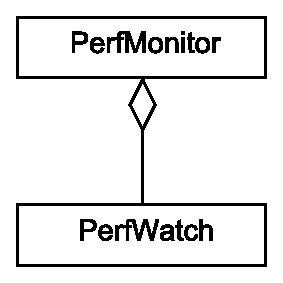
\includegraphics[width=0.15\textwidth]{PerfMonitor.eps}
\caption{計算性能測定機能 クラス図}
\label{fig:timing}
\end{center}
\end{figure}

PerfWatchクラスは,全てPerfMonitorクラスをとおして生成され操作されるので,
ソルバーから直接PerfWatchクラスのAPIを呼ぶことはない.

\subsubsection{PerfMonitorクラス公開メソッド}
\paragraph{初期化}\mbox{}\\
測定区間数({\tt nWatch})+1個の測定時計(PerfWatchクラス)をインスタンスして,
全計算時間用測定時計をスタートさせる.
測定区間を指定するキー番号は,0以上{\tt nWatch}未満である必要がある.
{\small
\begin{program}
void initialize(unsigned nWatch)
\end{program}
}

\paragraph{測定区間にプロパティを設定}\mbox{}\\
キー番号{\tt key}で識別される測定区間に,ラベル文字列{\tt label},
測定対象タイプ{\tt type}, 排他測定フラグ(true=排他測定/false=非排他測定)を設定.
{\small
\begin{program}
void setProperties(unsigned key, const string& label, Type type,
                   bool exclusive=true)
\end{program}
}

なお,測定対象タイプ{\tt type}の指定には,以下の定数を使用する.
\begin{quote}
\begin{description}
 \item[通信] {\tt PerfMonitor::COMM}   
 \item[計算] {\tt PerfMonitor::CALC}
\end{description}
\end{quote}

\paragraph{測定スタート}\mbox{}\\
キー番号{\tt key}で識別される測定区間の始まりを指定する.
{\small
\begin{program}
void start(unsigned key)
\end{program}
}

\paragraph{測定ストップ}\mbox{}\\
キー番号{\tt key}で識別される測定区間の終わりを指定する.
オプションとして,「タスク」あたりの計算量/通信量(バイト単位){\tt flopPerTask},
実行「タスク」数{\tt iterationCount}を申告できる.
{\small
\begin{program}
void stop(unsigned key, SKL_REAL flopPerTask=0.0, unsigned iterationCount=1)
\end{program}
}

\paragraph{測定結果の集約}\mbox{}\\
測定結果情報をノード0に集約し,統計情報を計算する.
また,初期化時にスタートさせた全計算時間用測定をストップさせる.
{\small
\begin{program}
void gather()
\end{program}
}

\paragraph{測定結果の出力}\mbox{}\\
排他測定区間についての統計情報を出力する.
ノード0以外では, 呼び出されてもなにもしない.
{\small
\begin{program}
void print(FILE* fp)
\end{program}
}

\paragraph{詳細な測定結果の出力}\mbox{}\\
非排他測定区間も含めて,詳細な統計情報を出力する.
ノード0以外では, 呼び出されてもなにもしない.
{\small
\begin{program}
void printDetail(FILE* fp)
\end{program}
}


\subsection{PerfMonitorクラスの使用方法}
PerfMonitorクラスを使用するには,
ヘッダファイルPerfMonitor.hインクルードする必要がある.

\paragraph{初期化}\mbox{}\\
以下の8ステップが必要:
\begin{enumerate}
\item インスタンス化
\item 測定番号識別キー番号定数の用意
\item setParallelInfoメソッドによる並列情報の設定
\item initializeメソッドによる測定区間数の登録
\item setPropertiesメソッドによる各測定区間へのプロパティの設定
\end{enumerate}

{\small
\begin{program}

  Parallel_Info pn;
  …
  // (1) インスタンス化
  PerfMonitor PM
  …
  // (2) 測定番号識別キー番号定数
  enum timing_key {
    tm_sec1,
    tm_sec2,
    … 
    tm_secN,
    tm_END_,   // ターミネータ(=測定区間総数)
  };

  …
  // (3) 並列情報設定
  PM.setParallelInfo(pn);

  // (4) 測定区間数の登録
  PM.initialize(tm_END_);

  // (5) 各測定区間にプロパティを設定
  PM.setProperties(tm_sec1, "SEC1", PerfMonitor::CALC);       //計算,排他
  PM.setProperties(tm_sec2, "SEC2", PerfMonitor::COMM);       //通信,排他
  PM.setProperties(tm_sec3, "SEC3", PerfMonitor::CALC, false);//計算,非排他
  …
\end{program}
}

\paragraph{測定区間の指定}\mbox{}
単純な指定では,
測定対象区間を同一キーを指定したstartメソッドとstopメソッドで挟む.
{\small
\begin{program}
  PM.start(tm_sec1);

  /* 測定対象区間 */

  PM.stop(tm_sec1);
\end{program}
}

以下の例では,測定対象区間内で
浮動小数計算量{\tt flop}のブロックを{\tt nStep}回実行していることを申告してる.
{\small
\begin{program}
  PM.start(tm_sec1);

  for (int i = 0; i < nStep; i++) {
    /* このブロックの浮動小数計算量が flop */
  }

  PM.stop(tm_sec1, flop, nStep);
\end{program}
}

\paragraph{測定結果の集計・出力}\mbox{}\\
測定結果出力メソッドを呼び出す前に,全ノードで集計メソッドgatherを呼び出す
必要がある.
出力メソッドはprintおよびprintDetailは,ノード0から呼ばれた時のみ
指定されたファイルへ測定結果情報を出力する.
{\small
\begin{program}
  // 測定結果の集計(gathreメソッドは全ノードで呼ぶこと)
  PM.gather();

  // コンソールへの測定結果の出力
  // (printとprintDetailメソッドはノード0以外は呼ばれても何もしない)
  PM.print(stdout);
  PM.printDetail(stdout);

  if (p.ID == 0) {
    FILE* fp = fopen("timing.txt", "w");

    // ファイルへの測定結果の出力
    // (printとprintDetailメソッドは, ノード0のみから呼び出してもOK)
    PM.print(fp);
    PM.printDetail(fp);

    fclose(fp);
  }
\end{program}
}

\paragraph{クラス変数TimingLevelによる測定レベル制御}\mbox{}\\
クラス変数TimingLevelの内容を
\[
\textrm{TimingLevel} = \left\{
\begin{array}{ll}
 0 & \textrm{測定なし}\\
 1 & \textrm{排他測定のみ実行}\\
 2 & \textrm{非排他測定も実行}
\end{array}
\right.
\]
と設定することにより,ヘッダファイルPerfMonitor.h内で定義された
2つのマクロPM\_TIMING\_\_,PM\_TIMING\_DETAIL\_\_をとおして,
ソルバー実行時の測定レベルを制御できる.
\begin{quote}
\begin{alltt}
#define PM_TIMING__         if (PerfMonitor::TimingLevel > 0)
#define PM_TIMING_DETAIL__  if (PerfMonitor::TimingLevel > 1)
\end{alltt}
\end{quote}

{\small
\begin{program}
   …
PM_TIMING__ { MO.start(...); }

   /* 排他測定区間 */

PM_TIMING__ { MO.stop(...); }
   …
   …
PM_TIMING_DETAIL_ { MO.start(...); }

   /*  非排他測定区間  */

PM_TIMING_DETAIL_ { MO.stop(...);
\end{program}
}

\subsection{統計情報出力内容}
\paragraph{printメソッド出力内容}\mbox{}\\
「{\tt Report of Timing Statistics}」に続いて
\begin{quote}
\begin{description}
\item[\tt Total execution time]\mbox{}\\
 ノード0における,initializeメソッド呼び出しからgatherメソッド呼び出しまでの時間
\item[\tt Total time of measured sections]\mbox{}\\
 全排他測定区間における「積算実行時間のノード間平均」の合計
\end{description}
\end{quote}
「{\tt Statistics per MPI process [Node Average]}」に続いて,各排他測定区間毎に
\begin{quote}
\begin{description}
\item[\tt call]\mbox{}\\
 測定回数(「startメソッド〜stopメソッド」ペアの呼び出し回数)
\item[\tt accumulated time]\mbox{}\\
 積算実行時間({\tt avr[sec]}はノード間平均値,
{\tt avr[\%]}は「{\tt Total time of measured sections}」値に対する平均値の割合,
{\tt sdv[sec]}は標準偏差,
{\tt avr/call[sec]}は1測定あたりの平均値)
\item[{\tt flop | messages[Bytes]}]\mbox{}\\
積算浮動小数演算量または通信量({\tt avr}はノード間平均値,
{\tt speed}は積算実行時間のノード間平均値より求めた計算速度または通信速度)
\end{description}
\end{quote}

なお,排他測定区間における測定回数がノード毎に異なっていた場合には,
その排他測定区間に関する統計情報の計算は行われず,「{\tt NA}」と出力される.

\paragraph{printDetailメソッド出力内容}
各測定区間,各ノード毎に,以下を出力
\begin{quote}
\begin{description}
\item[{\tt accm[s]}]\mbox{}\\
積算実行時間
\item[{\tt accm[\%]}]\mbox{}\\
積算実行時間の「{\tt Total time of measured sections}」値に対する割合
\item[{\tt waiting[s]}]\mbox{}\\
待ち時間(「積算実行時間のノード間最大値」と「積算実行時間」の差)
\item[{\tt accm/call[s]}]\mbox{}\\
1測定あたりの実行時間
\item[{\tt flop|msg}]\mbox{}\\
積算浮動小数演算量または通信量(バイト単位)
\item[speed]\mbox{}\\
積算実行時間より求めた計算速度または通信速度
\end{description}
\end{quote}

なお,非排他測定区間については,ラベル文字列をその前に「{\tt *}」をつけて表示する.









%
\chapter{データ保持クラス}
{\begin{abstract}
本章では,測定データを基に得られた実験式を条件とするような場合に利用するデータ保持機能について説明する.
\end{abstract}
\graphicspath{{./fig_DH/}}
%

\hypertarget{tgt:DH}{\section{時系列データ保持機能}}

時系列データ保持機能では,
ソルバー実行開始時に,指定されたファイル(入力データファイル)より
時系列データ(データセット)を読み込み,
ソルバー実行中にその値を参照できる機能を提供する.

入力データセットは時系列だけでなく,速度値に対する圧力損失値のように,
定義域が時間以外の物理量の場合にも対応可能である.
以下では便宜上,参照時にキーとなる量を「時刻」,参照したい量を「値」
と記すことにする.

データ値は,入力データセット毎に付けられたラベルと,時刻をキーにして
以下の規則により参照される.
\begin{itemize}
\item[-] 指定された時刻のデータがデータセット内に存在した場合,その時刻での値
\item[-] 指定された時刻がデータセット内の最小時刻より小さい場合,最小時刻データの値
\item[-] 指定された時刻がデータセット内の最大時刻より大きい場合,最大時刻データの
値
\item[-] その他の場合,指定された時刻を挟む2つの時刻データから,線形補間により値を計算
\end{itemize}



\subsection{XMLコンフィギュレーションファイルによる入力データファイル指定方法}
XMLコンフィギュレーションファイルのParameterセクションの
Data\_Holder要素内に,データセット数分のParam要素を記述する.
各Param要素には,name属性にデータの内容を表すラベル文字列を,
文字列型のvalue属性にデータファイルのパスを指定する.
ソルバー内部では,このラベル文字列によりデータセットの識別を行う.
{\small
\begin{program}
<Parameter>
  …
  <Elem name="Data_Holder">
    <Param name="label1" dtype="STRING" value="data/data1.dat" />
    <Param name="label2" dtype="STRING" value="data/data2.dat" />
  </Elem>
  …
</Parameter>
\end{program}
}
上例では,dataディレクトリの2つのデータファイルdata1.dat, data2.datを,
それぞれ「label1」「label2」というラベルを付けて指定している.


\subsection{入力データファイルのフォーマット}
入力データファイルは,テキストファイルとし,
各行に一組ずつ時刻と値を次の規則に従って記述する.
\begin{itemize}
\item[-] 時刻と値は,空白またはカンマで区切るものとする.
\item[-] 空白とは1つ以上の,半角スペースまたはタブである.
\item[-] 時刻の前,値の後ろ,カンマの前後に,空白を入れることもできる.
\item[-] 空行および「{\tt \#}」で始まるコメント行を任意の場所に挿入できる.
\item[-] 時刻と値の後ろに,さらに空白またはカンマを挟んでレコードが続く場合,
それらは無視される.
\end{itemize}
なお,時刻は昇順にソートされている必要はないが,同一時刻のデータが複数存在する場合にはエラーとして扱い,ソルバーの実行を停止する.

{\small
\begin{program}
#
# 1行に2つの実数「時刻」と「値」を空白またはカンマ区切りで記述
#
  時刻1   値1  # 空白区切り
  時刻2,値2    # カンマ区切り
  時刻3,  値3  # カンマ+空白区切り
   …       …
  時刻n   値n
\end{program}
}

\subsection{API説明}
時系列データ保持機能は,
個々のデータセットの内容を保持管理するDataHolderクラスと,
DataHolderクラス全体を管理するDataHolderManagerクラスからなる.
なお,DataHolderManagerクラスは,Parallel\_Nodeクラスから継承されている.
\begin{figure}[H]
\vspace{0.5cm}
\begin{center}
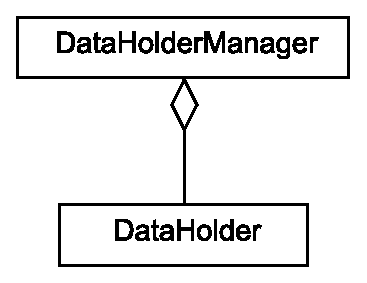
\includegraphics[width=0.18\textwidth]{DataHolder.eps}
\caption{時系列データ保持機能 クラス図}
\label{fig:data_holder}
\end{center}
\end{figure}

\subsubsection{DataHolderManagerクラス公開メソッド}

\paragraph{DataHolderの取得}\mbox{}\\
ラベル{\tt label}を指定して,対応するデータセットを保持管理している
DataHolderクラスオブジェクトへのポインタを返す.
対応するデータセットがない場合には0を返す.
{\small
\begin{program}
DataHolder* getDataHolder(const string& label)
\end{program}
}

\paragraph{DataHolder数の取得}\mbox{}\\
管理下にあるDataHolder数を返す.
{\small
\begin{program}
unsigned getNumDataHolder() const
\end{program}
}

\paragraph{DataHolder情報の出力}\mbox{}\\
管理下にある全DataHolderの情報を出力する.
{\small
\begin{program}
void printInfo(FILE* fp) const
\end{program}
}

\paragraph{DataHolder情報の出力(デバッグ用)}\mbox{}\\
管理下にある全DataHolderの情報(全データ内容を含む)を出力する.
{\small
\begin{program}
void printInfoDebug(FILE* fp) const
\end{program}
}

\paragraph{XMLファイルポインタの受け取り}\mbox{}\\
XMLコンフィギュレーションファイル({\tt SklCfg::SklSolverConfig}クラス)への
ポインタを受け取る.ポインタの内容が不正な場合,falseを返す.
{\small
\begin{program}
bool receiveCfgPtr(SlkCfg::SklSolverConfig* cfg)
\end{program}
}

\paragraph{データファイル読み込み}\mbox{}\\
XMLコンフィギュレーションファイルをパースし,入力データファイルを読み込み,
内部にDataHolderを生成し登録する.
{\small
\begin{program}
void readData()
\end{program}
}

\subsubsection{DataHolderクラス公開メソッド}
\paragraph{時刻を指定して値を取得}\mbox{}\\
指定された時刻{\tt t}に対して,格納データを参照して,線形補間により求めた値を返す.
指定された時刻が入力データの定義域外の場合には,最初あるいは最後の(最も近い時刻での)値を返す.
{\small
\begin{program}
SKL_REAL getValue(SKL_REAL t) const
SKL_REAL get_value(SKL_REAL t) const
\end{program}
}

\paragraph{データ値のスケーリング}\mbox{}\\
指定された倍率で,全時刻での値をスケーリングする.
データ値の単位変換などでの使用を想定している.
{\small
\begin{program}
void scale(SKL_REAL ratio)
\end{program}
}

\paragraph{時刻の最小値・最大値の取得}\mbox{}\\
時刻(データの定義域変数)の最小値・最大値を返す.
{\small
\begin{program}
SKL_REAL getMin() const
SKL_REAL getMax() const 
\end{program}
}

\paragraph{格納データ情報の出力}
格納データ情報(ラベル,ファイル名,データ数,時刻の最小値・最大値)を出力する.
{\small
\begin{program}
void printInfo(FILE* fp) const
\end{program}
}

\paragraph{格納データ情報の出力(デバッグ用)}
全格納データを出力する.
{\small
\begin{program}
void printInfoDebug(FILE* fp) const
\end{program}
}



\subsection{ソルバーへの組み込み方法}
DataHolderクラスおよびDataHolderManagerクラスを利用するには,
ヘッダファイルDataHolder.hをインクルードする必要がある.

\paragraph{初期化}\mbox{}\\
以下の4ステップが必要:
\begin{enumerate}
\item インスタンス化
\item setParallelInfoメソッドによる並列情報の設定
\item receiveCfgPtrメソッドによるXMLコンフィギュレーションファイルポインタの設定
\item readDataメソッドによる入力データファイルの読み込み
\end{enumerate}
\begin{program}
  Parallel_Info pn;
  SklCfg::SklSolverConfig* m_solvCfg;
  …
  // (1) インスタンス化
  DataHolderManager DH;   
  …
  // (2) 並列情報設定
  DH.setParallelInfo(pn);

  // (3) XMLコンフィギュレーションファイルポインタ設定
  if (!DH.receiveCfgPtr(m_solvCfg)) assert(0);

  // (4) 入力データファイル読み込み
  DH.readData();
\end{program}

\paragraph{データセットの参照}\mbox{}\\
以下の例のように,DataHolderクラスのポインタ変数を通して使う.
\begin{program}
  DataHolderManager DH;
  …
  /* ここでDHの初期化 */
  …
  // データセット「label1」へのポインタを取得
  DataHolder* data1 = DH.getDataHolder("label1");

  // エラー処理
  if (!data1) {
    printf("Error: no DataHolder labeled 'label1'.\n");
    …
  }

  SKL_REAL t = …;  // 時刻

  // 時刻tでの値を取得
  SKL_REAL x = data1->getVal(t);
\end{program}

また,次の例のように,DataHolderManagerのみを通して使うことも可能.
{\small
\begin{program}
  DataHolderManager DH;
  …
  /* ここでDHの初期化 */
  …
  SKL_REAL t = …;  // 時刻

  // データセット「label1」の時刻tでの値を取得
  SKL_REAL x = DH.getDataHolder("label1")->getVal(t);
\end{program}
}


%
\chapter{コンポーネントの実装}
\begin{abstract}
本章では,CBCソルバークラスにおけるコンポーネントの実装について説明する.
\end{abstract}
\graphicspath{{./fig_Implement/}}



%%
\section{内部境界条件の実装のしくみ}

%
\subsection{BC Index}
計算空間の各セルおよびセルの各フェイスへの境界条件処理は,機能性と計算効率の点で注意深く実装すべき部分である.
空間スキームのカーネル部分と比べて,条件分岐などが多くベクトル化,SIMD化が利きにくいため,計算量を最小化する工夫が必要となる.
境界条件の空間的存在範囲は局所的な傾向であり,その計算は並列処理時のロードバランスを崩す要因なので,この点にも気をつける必要がある.
CBCの実装方針として,以下のポリシを基本とする.

\begin{enumerate}
\item 局所的な処理\\
境界条件の存在範囲を探索する領域を最小化するため,BV情報を利用する.
\item 演算量を最小化\\
前処理可能な部分は,保存メモリ量も少なくするようにして保持する.
\item 2パス計算\\
通常の空間演算処理を行い,境界処理が必要な部分だけ計算し,修正量を加える.
\item 高性能計算\\
通常の空間演算処理においても,計算空間内の任意部分に現れる固体壁面の処理を効率よく行う工夫が必要になる.
また,反復計算において,係数行列のロードコストを削減することも高速計算に必要になる.
\end{enumerate}


CBCソルバでは,様々な境界条件の情報を纏めて管理し,計算時に境界条件を効率的に実装するため,\textbf{図\ref{fig:BCIndexDP}}および\textbf{図\ref{fig:BCIndexVH}}に示すBC Index,CompoList クラス,MaterialList クラスを利用する.
BC Indexは,計算処理に必要なフラグ情報を4バイトのビットフィールドに機能を持たせたフラグをコンパクトに割り当て,領域空間における境界条件の設定のために利用する.
CompoList クラスは境界条件の種類やパラメータなどの情報,MaterialList クラスはセル属性を保持する.

\begin{figure}[htbp]
\begin{center}
\includegraphics[height=11cm,clip]{BCindexDP.eps}
\end{center}
\caption{境界条件実装に用いるBC Index. bcd[]は共通要素,bcp[]は圧力計算に用いる.}
\label{fig:BCIndexDP}
\end{figure}

\begin{figure}[htbp]
\begin{center}
\includegraphics[height=11cm,clip]{BCindexVH.eps}
\end{center}
\caption{境界条件実装に用いるBC Index. bcv[]は速度計算,bch1, bch2[]は温度計算に用いる.}
\label{fig:BCIndexVH}
\end{figure}

bcd[]は計算空間を構成する各セルに対して割り当てられた配列で,\textbf{表\ref{tbl:Flags in bcd}}に示すように,共通的に利用する情報を保持する.
ComponentおよびMaterialは,それぞれ,CompoListとMaterialListクラスオブジェクト配列のエントリを格納する領域である.bh2[]でもCompoListへのエントリをエンコードするが,bcd[[]は全てのコンポーネントを保持する.一方,bh2[]では熱境界条件に必要なコンポーネントのみ保持する.
Cell IDはセルに割り当てられているIDを保持する.このIDはユーザが作成するボクセルモデルにより指定される.
Volume Fractionはセル内における流体の体積占有率を$0\sim255$の値で量子化した値を保持する.
Forcingは?.
Stateはセルの状態を指定するフラグで,排他的である.
Activeは対象セルが計算に有効かどうかを指定し,Kind\_of\_Solverの指定するモードにより異なる.

\begin{table}[htdp]
\caption{BC Index bcd[] に割り当てるビットフラグ(4バイト幅)}
\begin{center}
\small
\begin{tabular}{clll} \toprule
Bit & Flag & Property & Explanation\\ \midrule
31 & Active & 0-Invalid / 1-Valid & 対象セルが計算に有効かどうかを指定するフラグ\\
30 & State  & 0-Solid / 1-Fluid & セルの状態を指定するフラグ(排他的)\\
28 & Forcing & & \\
20$\sim$27 & Volume Fraction & 0-255 & 8bitで量子化された体積率[0,1]\\
12$\sim$19 & Cell ID & 1-255 & 8bit幅の正数\\
6$\sim$11 & Material & 1-63 & MaterialList[]へのエントリ(6bit幅)\\
0$\sim$5 & Component & 1-63 & CompoList[]へのエントリ(6bit幅)\\ \bottomrule
\end{tabular}
\end{center}
\label{tbl:Flags in bcd}
\end{table}

bcp[]は\textbf{表\ref{tbl:Flags in bcp}}に示すように,基本的に圧力計算に必要な情報を保持している.
No\_Sfaceは粘性項の修正に利用するための係数で実験的な実装である.
Facing\_?は,壁法則の計算などに利用するための情報で各セル方向に壁面があるかないかを示す.
BC\_Ndag\_?は反復計算時に利用する行列の対角要素の係数である.
BC\_Ndag\_?は同じく非対角要素の係数である.
BC\_N\_?とBC\_D\_?はぞれぞれ,Neumann条件とDirichlet条件のフラグであり,両者は同時に0ではありえない.

\begin{table}[htdp]
\caption{BC Index bcp[] に割り当てるビットフラグ(4バイト幅)}
\begin{center}
\small
\begin{tabular}{clll} \toprule
Bit & Flag & Property & Explanation\\ \midrule
31 & Active & 0-Invalid / 1-Valid & 対象セルが計算に有効かどうかを指定するフラグ\\
30 & State  & 0-Solid / 1-Fluid & セルの状態を指定するフラグ(排他的)\\
24$\sim$29 & BC\_D\_? & 0-Dirichlet / 1-Non Dirichlet(Default) & 各方向のセルフェイスのDirichlet境界フラグ\\
18$\sim$23 & BC\_N\_? & 0-Neumann / 1-Non Neumann(Default) & 各方向のセルフェイスのNeumann境界フラグ\\
12$\sim$17 & BC\_Ndag\_? & 0-境界条件あり / 1-境界条件なし & 各セルフェイス方向の係数\\
9$\sim$11 & BC\_Diag & [1-6] & 対角要素の係数\\
3$\sim$8 & Facing\_? & 0-壁面なし / 1-壁面あり & 各セルフェイス方向の壁面の有無(wall location)\\
0$\sim$2 & No\_Sface & [0-5] & セルの壁面の面数\\ \bottomrule
\end{tabular}
\end{center}
\label{tbl:Flags in bcp}
\end{table}

\textbf{表\ref{tbl:Flags in bcv}}に示すbcv[]は速度の計算に用いる境界条件情報である.
各方向に5bit幅\footnote{6方向$\times\,5bit\,<\,4B$}をもつ.0は境界条件がなく,標準スキームでの流束計算を行う.
1-30は境界条件でCompoList[]へのエントリを示す.
31は外部境界条件であることを示す.

\begin{table}[htdp]
\caption{BC Index bcv[] に割り当てるビットフラグ(4バイト幅)}
\begin{center}
\small
\begin{tabular}{clll} \toprule
Bit & Flag & Property & Explanation\\ \midrule
31 & Active & 0-Invalid / 1-Valid & 対象セルが計算に有効かどうかを指定するフラグ\\
30 & State  & 0-Solid / 1-Fluid & セルの状態を指定するフラグ(排他的)\\
25$\sim$29 & BC\_Face\_T & 0-BCなし / 1-30 エントリ / 31-外部BC & 各セルT方向のBC\\
20$\sim$24 & BC\_Face\_B & 0-BCなし / 1-30 エントリ / 31-外部BC & 各セルB方向のBC\\
15$\sim$19 & BC\_Face\_N & 0-BCなし / 1-30 エントリ / 31-外部BC & 各セルN方向のBC\\
10$\sim$14 & BC\_Face\_S & 0-BCなし / 1-30 エントリ / 31-外部BC & 各セルS方向のBC\\
5$\sim$9 & BC\_Face\_E & 0-BCなし / 1-30 エントリ / 31-外部BC & 各セルE方向のBC\\
0$\sim$4 & BC\_Face\_W & 0-BCなし / 1-30 エントリ / 31-外部BC & 各セルW方向のBC\\ \bottomrule
\end{tabular}
\end{center}
\label{tbl:Flags in bcv}
\end{table}


温度の計算に用いる境界条件情報のひとつbch1[]を\textbf{表\ref{tbl:Flags in bch1}}に示す.
各方向に5bit幅をもつ.0は境界条件がなく,標準スキームでの熱流束計算を行う.
1-30は境界条件でCompoList[]へのエントリを示す.
速度の場合と同様に,外部境界面上はコンポーネントの指定は行わない.

\begin{table}[htdp]
\caption{BC Index bch1[] に割り当てるビットフラグ(4バイト幅)}
\begin{center}
\small
\begin{tabular}{clll} \toprule
Bit & Flag & Property & Explanation\\ \midrule
31 & Active & 0-Invalid / 1-Valid & 対象セルが計算に有効かどうかを指定するフラグ\\
30 & State  & 0-Solid / 1-Fluid & セルの状態を指定するフラグ(排他的)\\
25$\sim$29 & BC\_Face\_T & 0-BCなし / 1-30 エントリ  & 各セルT方向のBC\\
20$\sim$24 & BC\_Face\_B & 0-BCなし / 1-30 エントリ  & 各セルB方向のBC\\
15$\sim$19 & BC\_Face\_N & 0-BCなし / 1-30 エントリ  & 各セルN方向のBC\\
10$\sim$14 & BC\_Face\_S & 0-BCなし / 1-30 エントリ  & 各セルS方向のBC\\
5$\sim$9 & BC\_Face\_E & 0-BCなし / 1-30 エントリ  & 各セルE方向のBC\\
0$\sim$4 & BC\_Face\_W & 0-BCなし / 1-30 エントリ  & 各セルW方向のBC\\ \bottomrule
\end{tabular}
\end{center}
\label{tbl:Flags in bch1}
\end{table}




\begin{table}[htdp]
\caption{BC Index bch2[] に割り当てるビットフラグ(4バイト幅)}
\begin{center}
\small
\begin{tabular}{clll} \toprule
Bit & Flag & Property & Explanation\\ \midrule
31 & Active & 0-Invalid / 1-Valid & 対象セルが計算に有効かどうかを指定するフラグ\\
30 & State  & 0-Solid / 1-Fluid & セルの状態を指定するフラグ(排他的)\\
24$\sim$29 & Adiabatic\_? & 0-断熱 / 1-非断熱  & 各フェイスの断熱指定状況\\
18$\sim$23 & GMA\_? & 0-BCあり / 1-BCなし  & 各フェイスの境界条件の有無\\
15$\sim$17 & H\_Diag & [1-6]  & 行列の対角要素の係数\\
5$\sim$15 & Blank &  & 未使用\\ 
0$\sim$4 & CompoList & 1$\sim$31 & 境界条件のエントリのみ\\ \bottomrule
\end{tabular}
\end{center}
\label{tbl:Flags in bch2}
\end{table}


%
\subsection{コンポーネント}
内部境界条件は,CBCソルバークラスのコンポーネントという概念で実装している.
コンポーネントは,ボクセルモデル内に設定されたIDの位置や付随する条件などを管理する機能である.
コンポーネントリストに登録されたIDは,境界条件やモニタ指定位置,媒質などの要素として利用される.

\subsubsection{内部境界条件の扱い}
熱流動解析の場合の境界条件を内部境界条件として指定する場合,通常,固体面側を基準に境界条件を与える.
これは,流体中で固体面が境界条件となることが多く,指定に便利なためである.
したがって,内部境界条件の指定時にキーとなるIDには固体セルを指定する.
一方で,固体熱伝導を解く場合には,熱流動解析とは逆に,流体面側を基準に境界条件を与える.

前処理の手順を以下に簡単に示し,後で詳述する.

\begin{enumerate}
\item セルIDの存在範囲の探索\\
ボクセルモデルのIDを探索して,コンポーネントの存在範囲のBV情報を得る.
このため\verb|getLocalCmpIdx()|内で,V-Sphereのメソッド\verb|GetBndIndexExtGc()|を用いてコンポーネントが存在する範囲のBV(Bounding Vox)を探索し,各ノード内のローカルインデクス情報を取得する.
つぎに,得られたBV情報から一層だけ拡大したインデクスを\verb|SklSolverCBC::getEnlargedIndex()|で\hyperlink{tgt:id search}{計算する}(\ref{sec:id search}参照).
一層拡大してBV情報を取得する理由は,キーとなるIDは固体セルであるが,境界条件の対象となるセルは固体IDに接する流体セルであるので,そのセルまで含めるためである.
グローバルインデクスはローカルインデクスから計算する.
グローバルなインデクスはソルバークラスのメンバ変数(\verb|int* GC_bv|)で管理し,ローカルなインデクスはコンポーネントクラスのメンバ変数(\verb|st[3], ed[3]|)で管理する.

\vspace{2mm}

\item ビットフラグのエンコード\\
BC Indexは,計算空間の各セルに対してunsigned int (4bytes)の変数が割当てられている.
この中に境界条件処理に関する情報をビットフィールドにエンコードする.
BC Index導入の目的は,諸情報をコンパクトに保持し,(1)メモリ領域の節約,(2)ロードコストを減らすことである.
BC Index にエンコードされるフラグは,境界条件設定時の空間ループ内の演算コストが小さくなるように実装する.
境界条件処理時のロードコストの削減が主目的であるので,\textbf{図\ref{fig:BCIndexDP}},\textbf{図\ref{fig:BCIndexVH}}に示すように,必要に応じて幾種類かのBC Indexを併用する.
\vspace{2mm}

\item コンポーネントBV情報の再構築\\
1の処理で,コンポーネントのBVは実際のコンポーネントの存在範囲の1つ外側を示していた.
2の処理で境界条件に必要な情報をエンコードし,実際に探索する範囲が確定した.
そこで,実行時の探索範囲を局所的に抑え,実行時間を短縮するため,BVインデクスを再度サーチし確定する.
探索には,境界条件処理で利用する探索アルゴリズム(BCindex情報を利用)を用いて,\verb|BinaryVoxel::resizeCompoBV()|により範囲を定める.

 再検索処理は,セルフェイス\verb|resizeBVface()|とセル要素\verb|resizeBVcell()|に対する2種類の処理がある.
処理手順は,\verb|setBCIndexP(),setBCIndexV(),setBCIndexH()|に倣う.
ここでは,ローカルインデクスとグローバルインデクスの両方を更新している.

\end{enumerate}

%
\hypertarget{tgt:id search}{\subsection{IDの探索処理}}
\label{sec:id search}

コンポーネントとして保持するIDについて,IDの存在範囲(BV, Bounding Vox)の算出方法について述べる.
IDのBV情報となる条件は,\textbf{キーIDが存在するBVを一層拡大した矩形範囲が自領域内にあること}である.
パターンとして,\textbf{図\ref{fig:ID BV}}に示すようなケースが考えられる.
領域内の最外側の層に対する処理を考えなければならないため,ガイドセル上のIDを考慮する必要がある.

\begin{figure}[htbp]
\begin{center}
\includegraphics[width=13cm,clip]{IDsearch.eps}
\end{center}
\caption{計算領域内に存在するIDのパターンとBV情報の計算.図中のa, dのハッチング部分は計算領域外なので,BVの対象外となる.一方,cのハッチング部分は,キーIDは領域\#0内,つまり領域 \#1から見るとガイドセル上にあるが,一層拡大した領域は\#1の領域内にあるため,BVの対象となる.}
\label{fig:ID BV}
\end{figure}

\begin{figure}[htbp]
\begin{center}
\includegraphics[width=13cm,clip]{IDpattern.eps}
\end{center}
\caption{一次元方向のIDの分布パターン.図ではガイドセル(g=2)と仮定している.処理は$(1)\sim(6)$の順番に行う.C indexからF indexへの変換は,$F_{idx} = C_{idx}+1-g$}.
\label{fig:ID pattern}
\end{figure}

一次元方向のIDのパターンを\textbf{図\ref{fig:ID pattern}}に示す.
最初に,対象IDのみが存在するBV情報は,V-Sphereのメソッド\verb|GetBndIndexExtGc()|で拡張オプションの引数0を渡して,ローカルなインデクス情報を得る.\verb|GetBndIndexExtGc()|は,各方向の開始インデクス\verb|st_i, st_j, st_k|とコンポーネントの長さ\verb|len_i, len_j, len_k|を返す.
このインデクス情報を初期値として,下記の各パターンに対して,一層拡大したインデクスを求め,所望のインデクス範囲\verb|st, ed|を得る.
以下,i方向について示す.インデクス\verb|st, ed|はFortranインデクスで保持する.
終了インデクスはCインデクスで次のように表せる.
{\small
\begin{program}
ed_i = st_i + len_i - 1;
\end{program}
}

\subsubsection{基本処理}
各ノード間のガイドセルを考慮した基本処理について示す.
以下の処理は,基本的に逐次の場合.並列時は,計算領域内か領域外かの判定が必要.
便宜的に次の変数を導入しておく.\verb|m_x|は三次元配列の各要素方向の最大値(計算内部領域)である.
{\small
\begin{program}
n_st = st_i - 1; // 一層外側へ拡大
n_ed = ed_i + 1; // 一層外側へ拡大
max_c1 = m_x + g;
\end{program}
}

また,以下のコンテキストで\verb|nID[]|には隣接6方向の各ノードのランク番号が入っており,隣接ノードがなければ負値が入っている.

\begin{description}
\item[(1)] BVがX-方向のガイドセル内のみにある場合\\
x+側に一層拡大し,その値が自領域内であれば,1層分だけ存在する.
{\small
\begin{program}
if ( ed_i < guide ) { 
  if( nID[MINUS_DIR] < 0 ){ // 計算領域の外部面に接する場合は,対象外
    m_st = 0;
    m_ed = 0;
  }
  else { // 計算領域内部にある場合(並列時)
    if ( n_ed == guide ) { // ガイドセル1層外側の場合
      m_st = 1; // F index
      m_ed = 1; // F index
    }
    else {
      m_st = 0;
      m_ed = 0;
    }
  }
}
\end{program}
}

\item[(2)] BVがX+方向のガイドセル内のみにある場合\\
x-側に一層拡大し,その値が自領域内であれば,1層分だけ存在する.
{\small
\begin{program}
if ( st_i >= max_c1 ) {
  if( nID[PLUS_DIR] < 0 ){ // 計算領域の外部面に接する場合は,対象外
    m_st = 0;
    m_ed = 0;
  }
  else {
    if ( n_st == (max_c1 - 1) ) { // ガイドセル1層外側の場合
      m_st = m_x; // F index
      m_ed = m_x; // F index
    }
    else {
      m_st = 0;
      m_ed = 0;
    }
  }
}
\end{program}
}

\item[(3)] BVが内部領域のみにある場合\\
開始点の処理は,x-側に一層拡大しその値が自領域内の端の場合,開始インデクスは領域内の最小インデクス.それ以外はマイナス1.
終点の処理は,x+側に一層拡大し,その値が自領域内の端の場合,終了インデクスは領域内の最大インデクス.それ以外はプラス1.
{\small
\begin{program}
if ( (st_i >= guide) && (ed_i < max_c1) ) {
  if ( st_i == guide ) { // 最外層セル
    m_st = 1; // F index
  }
  else {
    m_st = n_st + 1 - guide; // F index
  }
    
  if ( ed_i == (max_c1 - 1) ) { // 最外層セル
    m_ed = m_x; // F index
  }
  else { // 内部
    m_ed = n_ed + 1 - guide; // F index
  }
}
\end{program}
}

\item[(4)] BVが両方向のガイドセルにまたがる場合\\

{\small
\begin{program}
if ( (st_i < guide) && (ed_i >= max_c1) ) {
  m_st = 1; // F index
  m_ed = m_x; // F index
}
\end{program}
}

\item[(5)] BVがX-方向のガイドセルから内部領域にある場合\\
開始点は領域内の最小インデクス.終点は端点か,あるいは内部の可能性.
{\small
\begin{program}
if ( (st_i < guide) && (ed_i < max_c1) ) {
  m_st = 1; // F index
    
  if ( ed_i == (max_c1 - 1) ) { // 最外層セル
    m_ed = m_x; // F index
  }
  else { // 内部
    m_ed = n_ed + 1 - guide; // F index
  }
}
\end{program}
}

\item[(6)] BVがX+方向のガイドセルから内部領域にある場合\\
終点は領域内の最大インデクス.開始点は端点か,あるいは内部の可能性.
{\small
\begin{program}
if ( (st_i < max_c1) && (ed_i >= max_c1) ) {
  m_ed = m_x; // F index
    
  if ( st_i == guide ) { // 端点
    m_st = 1; // F index
  }
  else { // 内部
    m_st = n_st + 1 - guide; // F index
  }
}
\end{program}
}

\end{description}


上記のメソッドを各方向から利用できるように\verb|getEnlargedIndex()|を実装する.


%
\subsection{ビットフラグのエンコード処理}
BC Indexのビットフィールドへのエンコード処理を具体的に示す.

\begin{enumerate}
%
\item bcdへのエンコード(1) \verb|BinaryVoxel::setBCIndex_base1()|\\
BC Indexの配列bcd[]は,ソルバ中で共通的に利用するフラグを集めている.
ガイドセルを含む全領域に対して処理を行う.
まず,stateを流体で初期化.
次に,ボクセルモデルのセルIDを8bitでエンコードする\footnote{ID=0は使わないので,ID=1$\sim$255の範囲.}.
コンポーネントリストに登録された境界条件と媒質に対して,媒質情報にアクセスするためのMaterialList[]へのエントリをエンコードする.
最後に,各セルの媒質エントリをたどり,MaterialList[]の内容から流体か固体かを判断し,stateをエンコードする.
\vspace{2mm}

%
\item bcd[]へのエンコード(2) \verb|BinaryVoxel::setBCIndex_base2()|\\
先に設定したstateをみて,\verb|find_isolated_Fcell()|で孤立した流体セルを固体セルへ変更する.
これは,計算の不安定性を取り除くための処理で,大局的にみて影響は小さい.
この処理では,置換する固体セルは隣接固体IDの最頻値とする.

 次に,\verb|encActive()|で不活性セルの設定を行う.
不活性セルは,Kind\_of\_Solverのパラメータにより異なる処理となる.
\begin{itemize}
\item FLOW\_ONLY, THERMAL\_FLOW, THERMAL\_FLOW\_NATURAL\\
流体セルのみが計算に有効で,固体セルは不活性とする.

\item SOLID\_CONDUCTION\\
固体セルのみが計算に有効で,流体セルは不活性とする.

\item CONJUGATE\_HEAT\_TRANSFER\\
流体・固体セルともに有効.
\end{itemize}

さらに,コンポーネントで指定された不活性セルを不活性化する(Active bitをINACTIVEにする).
不活性セルの指定は,流体・固体セル両方可能.
\vspace{2mm}

%
\item bcp[]へのエンコード \verb|BinaryVoxel::setBCIndexP()|\\
bcd[]からactive, stateの両フラグをコピーし,残りのビットフラグを(1)で初期化する.
\vspace{2mm}

\begin{itemize}
\item 内部領域の処理 \verb|encPbit_Wall_Inside()|\\
内部領域にある流体セルのうち,固体セルに隣接する面のノイマンフラグ\verb|BC_N_?|をゼロにする.
外部境界面に接するセル面は後で処理.
つぎに,全内部領域について,固体セルに隣接する流体セルにwall locationフラグを付与する.
この処理は,\verb|cbc_pvec_()|などの関数で壁法則の計算に利用する.
\vspace{2mm}

\item 外部境界面の処理 \verb|BinaryVoxel::encPbit_OBC()|\\
外部境界面がDirichletかNeumannかを指定し,対応するフラグ\verb|BC_D_?|または\verb|BC_N_?|をエンコードする.
外部境界面が壁面の場合にのみ,方向フラグを付与する.
\vspace{2mm}

\item コンポーネントのエンコード\\
コンポーネントの境界条件の種類毎に処理の内容は異なる.
\begin{itemize}
\item SPEC\_VEL, SPEC\_VEL\_WH, OUTFLOW\\
テストセルが流体セルでDef\_Face IDが指定されている場合,かつ,テストセルの隣接セルが固体でキーIDの場合,テストセルの対象面にNeumannフラグをエンコードし,bcd[]にComponentList[]へのエントリを登録する.
\vspace{2mm}

\item PERIODIC, CELL\_MONITOR, IBM\_DF, HEX, FAN, DARCY\\
bcd[]にComponentList[]へのエントリを登録する処理のみ行う.
\vspace{2mm}

\end{itemize}

\item 対角・非対角要素の係数のエンコード \verb|encPbit()|\\
NeumannフラグとDirichletフラグが同時に設定されていないことを確認.
反復行列の非対角要素/対角要素をエンコードする.
対角要素がゼロの場合はエラー.
\end{itemize}
\vspace{2mm}

%
\item bcv[]へのエンコード \verb|BinaryVoxel::setBCIndexV()|\\
速度境界条件の種類をセルの各面にエンコードする.
各面に5bitを割り当てる.(0)は境界条件なし,(31)は外部境界条件,それ以外の(1$\sim$30)はコンポーネントのエントリを示す.
まず,bcd[]からactive, stateの両フラグをコピーする.

\begin{itemize}
\item 外部境界面の境界条件のエンコード \verb|BinaryVoxel::encVbit_OBC()|\\
この処理は,外部境界面に接するセルが流体の場合を対象とする.
外部境界条件の実装には,流束形式と境界値形式の2種類がある.
流束形式はOBC\_SYMMETRIC, OBC\_WALL, OBC\_SPEC\_VEL, OBC\_OUTFLOWで,境界値形式はOBC\_TRC\_FREE, OBC\_PERIODIC, OBC\_IN\_OUTである.
流束形式の場合には,セルフェイスに外部境界条件フラグ(31)をエンコードする\footnote{運動量fluxの計算で,セルフェイスが境界条件(!=0)の場合には,その流束の寄与をゼロにしておいて,後ほど境界条件による流束を加算する.}.
OBC\_SYMMETRIC, OBC\_WALLのときガイドセルが固体であることをチェックし,
OBC\_SPEC\_VEL, OBC\_OUTFLOWのとき対象セルが流体の場合のみガイドセルが流体であることをチェックする.

 境界値形式のOBC\_TRC\_FREE, OBC\_IN\_OUTの場合,対象面が流体であることのみチェックし,セルフェイスに外部境界条件フラグはエンコードしない.
つまり,通常スキームによる計算となる.
OBC\_PERIODICの場合には,外部境界条件フラグのエンコードも流体面のチェックも行わない.
\vspace{2mm}

\item 内部境界条件のコンポーネントへのエンコード \verb|BinaryVoxel::encVbit_IBC()|\\
コンポーネントがSPEC\_VEL\_WH, SPEC\_VEL, OUTFLOWの場合,キーIDは固体セル,Def\_Face IDに流体セルが指定される.
したがって,テストセルが流体でDef\_Face IDが指定され,かつ,テストセルの隣接セルが固体でキーIDの場合にのみ,エンコード処理を行う.
また,流体セルの流入出面にはコンポーネントのエントリをエンコードし,同時にbcp[]の壁面方向を表すwall locationフラグをoffにする.
これは,境界条件付与部分の固体面は,壁法則の計算を行わないようにするためである.

 内部境界条件の流入出は,ボクセルモデルでは固体セルにより流入出面が規定されている.\hyperlink{tgt:inflow}{流入出境界条件処理}で高次風上スキーム時の運動量流束の正確な計算のため,指定されたキーIDのセルを流体の状態にしておく.
\vspace{2mm}

\item セルの固体面数のエンコード \verb|encPbit_No_SolidFace()|\\
bcp[]にセルの6面のうち,固体面の数をエンコードする\footnote{粘性項の表面積補正のための実験的実装.}.
もし,6面とも固体面の場合にはエラーで停止する.

\end{itemize}

%
\vspace{2mm}

\item bch1, bch2へのエンコード \verb|BinaryVoxel::setBCIndexH()|\\
温度境界条件の情報をエンコードする.
bcd[]からactive, stateの両フラグをコピーする.
\vspace{2mm}

\begin{itemize}
\item 断熱フラグの初期化\\
bch2[]の断熱フラグを非断熱(1)に初期化する.
\vspace{2mm}

\item Kind\_of\_Solverのパラメータに応じて,Solid-Fluid面の断熱処理\\
THERMAL\_FLOW, THERMAL\_FLOW\_NATURALの場合,FluidセルのうちSolidセルに接する面について,\verb|setAmask_Thermal()|でbch2[]の断熱フラグを断熱(0)にする.
SOLID\_CONDUCTIONの場合,SolidセルのうちFluidセルに接する面について,\verb|setAmask_Solid()|でbch2[]の断熱フラグを断熱(0)にする.
\vspace{2mm}

\item 対称境界面に断熱マスクをセット\\
対称境界が指定された外部境界面に対して,\verb|encAmask_SymtrcBC()|でbch2[]の断熱フラグを断熱(0)にする.
\vspace{2mm}

\item 不活性セルの場合の断熱マスク処理\\
コンポーネントで指定された不活性セルIDに対して,\verb|setAmask_InActive()|でセルをInactiveにする.
流体セル,固体セルに関わらず,隣接セルがInactive指定の場合には断熱にするが,自セルが指定ID以外のときに限る.
つまり,Inactiveに指定したセルと接するセルの隣接面を断熱にする.ただし,隣接セルは非Inactive指定であること.
これは,Inactive指定セルが塊の時には,その内部はラプラスを解き,平均場にするため.
\vspace{2mm}

\item コンポーネントのエンコード\\
各コンポーネント毎の処理を行う.
\vspace{2mm}

\begin{description}
\item[-] 断熱条件 \verb|encQface()|\\
テストセルがDef\_Faceで,隣接セルがキーIDのセルで挟まれる面に対して,bch1[]にCompoListのエントリをエンコードし,
bch2[]に断熱条件(0)をエンコード.
\vspace{2mm}

\item[-] 熱流束指定 \verb|encQface()|\\
テストセルがDef\_Faceで,隣接セルがキーIDのセルで挟まれる面に対して,bch1[]にCompoListのエントリをエンコードし,
bch2[]に非断熱条件(1)をエンコード.
\vspace{2mm}

\item[-] 流入・流出指定 \verb|encQfaceSVO()|\\
コンポーネントがSPEC\_VEL\_WH, OUTFLOWの場合,キーIDは固体セル,Def\_Face IDに流体セルが指定される.
テストセルがDef\_Face IDで指定され,かつ,隣接セルがキーIDの場合にのみ,
bch1[]にCompoListのエントリをエンコードし,bch2[]に非断熱条件(1)をエンコードする.\verb|BinaryVoxel::encVbit_IBC()|の場合とは異なり,セルの状態をチェックしない.
\hyperlink{tgt:inflow}{流入出境界条件処理}で高次風上スキーム時の対流熱流束の正確な計算のため,指定されたキーIDのセルを流体の状態にしておく.
\vspace{2mm}

\item[-] 熱伝達指定 Type\_S \verb|encQfaceHT_S()|\\
Kind\_of\_SolverがTHERMAL\_FLOWまたはTHERMAL\_FLOW\_NATURALの場合に,コンポーネントHeatTransfer\_S, HeatTransfer\_SN,HeatTransfer\_SFを指定できる.
キーIDは固体セル,Def\_Face IDに流体セルが指定される.
テストセルがDef\_Face IDかつ流体で指定され,かつ,隣接セルがキーIDかつ固体の場合にのみ,
bch1[]にCompoListのエントリをエンコードし,bch2[]に非断熱条件(1)をエンコードする.
\vspace{2mm}

\item[-] 熱伝達指定 Type\_B \verb|encQfaceHT_B()|\\
Kind\_of\_SolverがCONJUGATE\_HEAT\_TRANSFERまたはSOLID\_CONDUCTIONの場合に,コンポーネントHeatTransfer\_Bを指定できる.
キーIDは固体セル,Def\_Face IDに流体セルが指定される.
テストセルがキーIDかつ固体で指定され,かつ,隣接セルがDef\_Faceかつ流体の場合にのみ,
bch1[]にCompoListのエントリをエンコードし,bch2[]に非断熱条件(1)をエンコードする.
\vspace{2mm}

\item[-] 等温指定 \verb|encQfaceISO_SF/SS()|\\
等温境界条件は,流体と固体,あるいは固体と固体で挟まれる面に対して適用可能である.
流体と固体セルの間で指定される等温境界は,Kind\_of\_SolverがTHERMAL\_FLOWまたはTHERMAL\_FLOW\_NATURALの場合に用いられる.
このとき,キーIDに固体セル,Def\_Face IDには流体セルが指定される.
テストセルがDef\_Face IDかつ流体で指定され,かつ,隣接セルがキーIDかつ固体の場合に,bch1[]にCompoListのエントリをエンコードし,bch2[]に非断熱条件(1)をエンコードする.

 一方,固体セル間の面で指定される等温境界は,Kind\_of\_SolverがCONJUGATE\_HEAT\_TRANSFERまたはSOLID\_CONDUCTIONの場合に用いられる.
このとき,キーIDセルとDef\_Face IDセルは両方とも固体セルである.
テストセルがキーIDかつ固体で,Def\_Face ID(固体セル)と挟まれる面に対して,bch1[]にCompoListのエントリをエンコードし,bch2[]に非断熱条件(1)をエンコードする.
\vspace{2mm}

\item[-] 熱源指定\\
熱源のタイプとして,Heat\_SourceとConstant\_Temperatureの2種類の指定方法がある.
これらの境界条件は,体積要素に対する指定である.
テストセルが指定されるIDの場合,bch2[]にCompoListのエントリをエンコードする.

\end{description}

\vspace{2mm}

\item 熱境界フラグの設定 \verb|encHbit()|\\
GMA\_?のフラグをセットする.まず,(1)で初期化.
bch1[]の各セルフェイスフラグBC\_FACE\_?をみて,境界条件があればbch2[]のGMA\_?を(0)にする.
その後,対角要素の係数を断熱マスクを考慮して計算し,H\_DIAGに対角要素の係数(0$\sim6$)をストアする.
もし,対角要素が(0)であればゼロ割防止のために(1)を入れておく.対角要素がゼロのセルは境界条件や断熱セルで囲まれたセルに相当する.
\end{itemize}


%
\vspace{2mm}

\end{enumerate}





BC Index bx[] は図\ref{fig:Decode}を参照して下記のコードのように利用する.この例では速度の境界条件について説明している.まず,setInnerVBCface()で境界条件のループnを回し,それがフェイス面に対する速度境界条件であれば(isVBCF()),処理を行う.次に,cmp[n].getType()の値により,n番目に登録された境界条件の種類を特定する.その後,個別の処理を行う.setDirichletVInside()では,指定された面に速度成分を与える処理を行っている.空間ループを回し,bx[i,j,k] の値がエンコードされた境界条件の格納番号,および方向と一致する場合に目的の処理を行う.このとき,必要に応じて MaterialListに登録された物性値を利用する.

{
\small
\begin{verbatim}
/**
 @fn void SetBC3D::setInnerVBCface(SKL_REAL* v, unsigned* bx, SKL_REAL v00, ...)
 @brief 速度の内部境界をセットする
 @param v 速度ベクトル
 @param bx BCindex
 @param v00 基準速度情報
 @param tm 時刻
 @param arrangement 格子配置
 */
void SetBC3D::setInnerVBCface(SKL_REAL* v, unsigned* bx, SKL_REAL v00, 
                                      SKL_REAL tm, const char* arrangement)
{
  for (unsigned n=1; n<=NoBC; n++) {
    if ( cmp[n].isVBCF() ) {

      switch ( cmp[n].getType() ) {
        case DIRICHLET_INSIDE:
				case DIRICHLET_CTMP:
          if ( !strcasecmp("staggered", arrangement)) {
            if ( cmp[n].usw != DRC_V_SHO ) {
                  cmp[n].val[0] = setDirichletV_Inside_S(v, bx, n, v00);
            }
            else {
                  cmp[n].val[0] = setSHO_Inside_S(v, bx, n, tm, v00);
            }
          }
          else if ( !strcasecmp("collocated", arrangement)) {
            ;
          }
          else {
            stmpd_printf("Invalid keyword\n");
          }
          break;
          
        default:
          break;
      }

    }
  }
}

/**
 @fn SKL_REAL SetBC3D::setDirichletVInside(SKL_REAL* v, unsigned* bx, unsigned n, SKL_REAL v00)
 @brief 内部領域の速度のディリクレ境界をセットする
 @param v 速度ベクトル
 @param bx BCindex
 @param n 境界条件コンポーネントのエントリ番号
 @param v00 参照速度
 @retval 無次元平均流速
 @note
    - 内部境界はセル面直を仮定
 */
SKL_REAL SetBC3D::setDirichletV_Inside_S(SKL_REAL* v, unsigned* bx, unsigned n, SKL_REAL v00)
{
  unsigned i, j, k, s;
  SKL_REAL va=0.0;
  SKL_REAL vel, vec[3];
  
  vel   = cmp[n].N1.Velocity * v00;
  
  vec[0]= cmp[n].nv[0]*vel;
  vec[1]= cmp[n].nv[1]*vel;
  vec[2]= cmp[n].nv[2]*vel;
  
  for (k=cmp[n].ci.st[2]; k<=cmp[n].ci.ed[2]; k++) {
    for (j=cmp[n].ci.st[1]; j<=cmp[n].ci.ed[1]; j++) {
      for (i=cmp[n].ci.st[0]; i<=cmp[n].ci.ed[0]; i++) {
        s = bx[ SklUtil::getFindexS3D(size, guide, i, j, k) ];
        if ( FBUtility::chkBCOrder(s, n) ) {
          if ( FBUtility::chkShift(s, VFACE_I) ) {
            va += v[SklUtil::getFindexV3D(size, guide, i, j, k, 0)] = vec[0];
          }
          if ( FBUtility::chkShift(s, VFACE_J) ) {
            va += v[SklUtil::getFindexV3D(size, guide, i, j, k, 1)] = vec[1];
          }
          if ( FBUtility::chkShift(s, VFACE_K) ) {
            va += v[SklUtil::getFindexV3D(size, guide, i, j, k, 2)] = vec[2];
          }
        }
      }
    }
  }
  va = va * dh*dh / (SKL_REAL)cmp[n].area;
  return (va);
}
\end{verbatim}
}

\begin{figure}[htbp]
\begin{center}
\includegraphics[width=12cm,clip]{Decode.eps}
\end{center}
\caption{BC Indexからのビットフラグのデコード}
\label{fig:Decode}
\end{figure}


%
\subsection{セルフェイスに対する速度境界条件}
スタガード変数配置における各速度成分に対して値を指定する.例として,図\ref{fig:cell face BC}に示すようなバイナリボクセルモデルにおいて,矢印方向の速度成分を与えることを考える.IDとして,空間に1, 3が指定されている.このとき,矢印の方向ベクトルは(0,1,0)でID=3とID=1が接する面であるので,以下のようなXMLで大きさ0.58の一定な速度成分を指定する.

\begin{figure}[htbp]
\begin{center}
\includegraphics[width=8cm,clip]{Vface-mid.eps}
\end{center}
\caption{セルフェイスにおける速度境界条件}
\label{fig:cell face BC}
\end{figure}

{
\small
\begin{verbatim}
<InnerBoundary>
  <Elem name="Vec_Face" id="1">
    <Elem name="Dirichlet" id="3" comment="source">
      <Param name="Norm_x"      dtype="REAL"   value="0.0" />
      <Param name="Norm_y"      dtype="REAL"   value="1.0" />
      <Param name="Norm_z"      dtype="REAL"   value="0.0" />
      <Param name="velocity"    dtype="REAL"   value="0.58" />
      <Param name="def_face"    dtype="INT"    value="1" />
      <param name="type"        dtype="string" value="constant" />
    </Elem>
  </Elem>
</InnerBoundary>
\end{verbatim}
}

%
\subsection{セルフェイスに対する熱境界条件}
\begin{indentation}{3zw}{0zw}
{
熱境界条件をコンポーネントとして与える場合,基本的に,固体面に与える.
\textbf{図\ref{fig:heat bc on solid}}に示すように,固体面から流体側へ法線を考えて,法線方向が指定値の正の値とする.
つまり,流体側への熱移動が正の方向となるように考える.

\begin{figure}[htbp]
\begin{center}
\includegraphics[width=6cm,clip]{heatBC.eps}
\end{center}
\caption{流体-固体界面における熱境界条件の指定方法}
\label{fig:heat bc on solid}
\end{figure}

この考え方に基づくと,Solver\_PropertyのKind\_of\_Solverの指定モードによって,熱境界条件の働きが異なる.
Thermal\_FlowとThermal\_Flow\_Naturalの場合は,熱流動計算で流体の温度のみが意味を持ち,固体部分は計算対象とはならず不活性セルとして扱う.
したがって,流体-固体の境界面で与える熱境界条件(熱流束)は,流体セル側のみに指定する.

一方,Solid\_Conductionの場合は固体部分の熱伝導のみを解くので,流体部分は不活性セルとして扱う.
したがって,流体-固体の境界面で与える熱境界条件は,固体セル側のみに指定する.

また,Conjugate\_Heat\_Transferの場合には流体と固体の熱移動を計算する.
したがって,流体-固体の境界面で与える熱境界条件は,流体セルと固体セルの両方で指定する.

以下の各境界指定で述べるように,IDとDef\_Faceタグの組み合わせにより,流体-固体の境界面を指定する.
このとき,IDには固体のIDを,Def\_Faceには流体または固体のIDを指定することを基本とする\footnote{IDに固体を指定する理由は,固体面は大抵の場合局所的なので,参照範囲を小さく抑えて効率的な計算をするため.}.


境界条件の処理手順は次のとおり.
\begin{enumerate}
\item \verb|SetBC3D::InnerTBCface()|\\
拡散項に関するセルフェイスの熱境界条件処理.
コンポーネントのループを回し,対象境界条件を特定し,各処理に分岐.
熱流束指定の場合には\verb|SetBC3D::ps_IBC_Heatflux()|で境界条件を計算.
戻り値をコンポーネントのモニタ保持変数に代入.
\vspace{2mm}

\item \verb|SetBC3D::ps_IBC_Heatflux()|\\
与える熱流束を有次元から無次元に変換.
各コンポーネントリストのBVループ範囲のセルに対して,セルを構成する各面に境界条件が指定されているかどうかをテストする.
対象となる面に対しては,熱流束を保持する配列\verb|qbc|に値をストアする.
スタガードのインデクスに注意.
セルのW面における正値$(q \ge 0)$は流入で,E面における正値$(q \ge 0)$は流出となる.
この関数内でallreduce()をかけ,無次元熱流束を集約,返値にする.
\end{enumerate}


上記の処理を行うための前処理として,次の処理を行っておく.
\begin{enumerate}
\item \verb|BinaryVoxel::setBCIndexH()|\\
熱境界条件のビットインデクスをエンコードする.
\begin{itemize}
\item まず,セルの各面の断熱マスク(6面分)を非断熱(1)に初期化する.
\item モードに応じて,流体-固体界面を断熱(0)にする.
\begin{description}
\item[-] THERMAL\_FLOWとTHERMAL\_FLOW\_NATURALの場合,\verb|BinaryVoxel::setAmask_Thermal()|で,S-F面のF側を断熱にする.
\item[-] SOLID\_CONDUCTIONの場合は,\verb|BinaryVoxel::setAmask_Solid()|で,S-F面のS側を断熱にする.
\item[-] CONJUGATE\_HEAT\_TRANSFERの場合には,固体セルも流体セルも両方とも計算するので,断熱処理はしない.
\end{description}

\item 対称境界面に断熱マスクをセット\\
\item 不活性セルの場合の断熱マスク処理\\
\item 媒質コンポーネントに対して,elementをセット\\
\item 具体的なエンコード処理\\
\item 係数行列の値をビットでエンコード\\
\verb|BinaryVoxel::encHbit()|で,\verb|bh2[]|の$\gamma$を1で初期化.
\verb|bh1[]|を調べて,セルの各面に境界条件がセットされていなければ(!=0),\verb|bh2[]|の各面で$\gamma=1$とする.
対角要素の係数は$\sum \limits_j=0^5 \left( \gamma_{BC} \gamma_A \right)_j$として,断熱マスクを考慮.
\end{itemize}



\vspace{2mm}

\item 
\end{enumerate}



\vspace{20mm}

ボクセルモデルのセルフェイスに対する熱境界条件 QBC\_Face の具体的な種類は,XMLファイルに記述された内容を基にしてCompoList クラスのオブジェクトのメンバー変数,compo[n].type にエンコードする.

図\ref{fig:BCIndex}のBC Index の$17\sim22$ビットにおいて,セルの6面に対して BC の種類を判別するフラグを持たせるのは,隣接セルとの重複があるため冗長であるが,BC Index の値をロードした後ビット演算だけで済む.よって,メモリアクセスが少ないので効率が良い.
セル P の全てのプラス方向の面に対してエンコード処理を行い,その後プラス方向の面の情報を隣のセルのマイナス方向にコピーする.

BCフラグの値は,下記の疑似コードのように利用する.
{
\small
\begin{verbatim}
/**
 @fn void FBUtility::getBCgamma (unsigned idx, SKL_REAL* a)
 @brief γの値から係数を配列で返す
 @retval γ
 @param idx BCindex
 @param a 係数配列
 */
void FBUtility::getBCgamma(unsigned idx, SKL_REAL* a) 
{
  a[0] =(SKL_REAL)( (idx >> GMA_W) & 0x1 );
  a[1] =(SKL_REAL)( (idx >> GMA_E) & 0x1 );
  a[2] =(SKL_REAL)( (idx >> GMA_S) & 0x1 );
  a[3] =(SKL_REAL)( (idx >> GMA_N) & 0x1 );
  a[4] =(SKL_REAL)( (idx >> GMA_B) & 0x1 );
  a[5] =(SKL_REAL)( (idx >> GMA_T) & 0x1 );
}
\end{verbatim}
}
QBC\_Face の具体的な境界条件は,前述のXMLファイルに記述された内容を基に判断する.
次節以降で具体的な境界条件について述べる.
}
\end{indentation}







%
\subsection{外力を用いた境界条件の実装}
\label{sec:implementation external force}
\ref{sec:external force method}で説明した外力項による境界条件について,その実装を説明する.



%
\subsection{Immersed Boundaryを用いた境界条件の実装}
\label{sec:implementation of IB}

\ref{sec:Immersed Boundary Method}で述べたImmersed Boundary Methodの実装について説明する.計算する格子系としては,StaggeredとCollocatedの2種類がある.そのため,前処理では格子配置に応じて内部処理が異なる.図\ref{fig:IBmask}に示すように,変数配置により指定したセル領域内にかかる速度定義点が異なる.このため,Staggeredではセル境界に与える境界条件VBCFで記述し,Collocatedではセルセンターに与える境界条件VBCCで記述する.
Staggeredの場合には,セルに与えられたDirect\_ForcingのIDを見つけると,そのセルの両端にあるセル界面位置の速度定義点をForcingの対象とする.これに対して,Collocatedの場合には,セルセンターの速度定義点のみがForcingの対象となる.

解法で述べたように,Direct Forcingは速度の強制で実装するので,内部的にはディリクレ型速度境界条件を使って実装する.
また,Direct Forcingは流体セルに対して有効であるので,Active\_BitはONにしておく.

\begin{figure}[htbp]
\begin{center}
\includegraphics[width=8cm,clip]{IB_mask.eps}
\caption{Direct Forcningのセル指定と強制対象となる速度位置の関係}
\label{fig:IBmask}
\end{center}
\end{figure}


%
\subsection{V-Sphereコンポーネントを用いた実装}
全計算領域の一部に存在する内部境界条件要素(コンポーネント)の実装にV-Sphereにより提供されるComponent機能を用いる.この機能には,並列処理時のサブドメイン間のデータ通信や管理が含まれ,均等分割とマルチボックス分割の両方に対応する.

\begin{enumerate}
\item 全計算領域のボクセル情報の初期化\\ 
\verb|SklSolverC3D::VoxelInitialize()|
\item Bounding Boxのグローバル情報の取得\\ 
\verb|SklSolverC3D::getGlobalCmpIdx_SubVoxInit()|
\item コンポーネント領域の初期化と登録\\ 
\verb|SklSolverC3D::getGlobalCmpIdx_SubVoxInit()|
\item コンポーネントへのデータクラスの追加\\ 
\verb|SklSolverC3D::allocArray_forcing (long &total, int para_key)|\\
dc\_bsi(スカラ), dc\_cfr(ベクトル)のデータクラスをコンポーネントでインスタンスする.
\item コンポーネントの存在するセルに体積率を与える\\
\verb|BinaryVoxel::setCmpFractionBV()|
dc\_cfrに体積率を保持する.
\end{enumerate}



%
\section{境界条件}
境界条件の本体は主にFortran90で記述している.Fortran コードは,C++の名前空間内ではCソースコードと同様に名前なし空間として扱われるので,FortranFuncC3D.h内にプロトタイプを記述しておく.

\subsection{外部境界条件の実装}
外部境界条件は,計算領域の外周に設定する境界条件である.
各節で,速度,圧力,温度に対する境界条件を説明する.
Fortranコードは,SetBC3Dクラスに実装されたメソッドsetOuterPBC, SetOuterTBC, setOuterVBC内でハンドリングされている.
Fortranコードには,たとえば流出境界条件ならば,計算領域の$X\pm$面,$Y\pm$面,$Z\pm$面の各面に対する処理が書かれている.
このサブルーチンをコールするときに,方向と必要なパラメータをセットすることで必要な面の境界条件を設定する.

\begin{verbatim}
#define X_MINUS 0
#define X_PLUS  1
#define Y_MINUS 2
#define Y_PLUS  3
#define Z_MINUS 4
#define Z_PLUS  5
\end{verbatim}



%
\section{温度輸送方程式の実装}
\subsection{Euler陽解法}
式(\ref{eq:pscalar ee2})を$\Delta$形式にして解く.

\begin{equation}
\theta^{n+1} \,=\, \theta^{n} \,+\, \Delta \theta^{n+1}
\label{eq:delta form 1}
\end{equation}

\begin{equation}
\Delta \theta^{n+1} \,=\, \Delta t \, f \left( u_{i}, \, \theta \right)
\label{eq:delta form 2}
\end{equation}

式(\ref{eq:delta form 2})の$f \left( u_{i}, \, \theta \right)$は式(\ref{eq:pscalar ee2})の右辺である.
\verb|SklSolverCBC::PS_E_CBS()|メソッド内では,次のように実装している.

\begin{enumerate}
\item 対流熱流束の計算\\
\verb|cbc_tfx_cnv_uwd_()|または\verb|cbc_tfx_cnv_muscl_()|で対流熱流束を求める.流入境界条件を指定している場合には,計算した対流熱流束に上書きする形で与えている.
\item 対流項の増分\\
ConvectionEE()で対流項の増分を計算する.
\item 境界条件\\

\end{enumerate}






%
\chapter{Appendix}
\graphicspath{{./fig_APDX/}}
%

\section{回転行列}

%
\subsection{回転行列の性質}
回転行列の一般的な性質について述べる~\cite{shimada:00:cadcg, ohishi:94:graphics}.
ある座標$\bm p$が原点を通る回転軸によって回転して$\bm q$に移動する状態変化は,回転行列$\bm T$を用いて,

\begin{equation}
\bm q \,=\, \bm{T\,p}
\label{eq:trans-matrix}
\end{equation}

ただし,
\begin{equation}
\bm T \,=\, \left[
\begin{array}{ccc}
a_1 & b_1 & c_1 \\
a_2 & b_2 & c_2 \\
a_3 & b_3 & c_3 
\end{array}
\right] \,=\, (\bm a,\, \bm b,\, \bm c)
\label{eq:matrix def}
\end{equation}

また,行列$\bm T$は,

\begin{equation}
\bm T \,=\, \bm{ai} + \bm{bj} + \bm{ck}
\label{eq:matrixT}
\end{equation}

つまり,ある座標軸を表すベクトル$(\bm i,\, \bm j,\, \bm k)$を,それぞれベクトル$(\bm a,\, \bm b,\, \bm c)$に変換することを意味している\footnote{ここで,扱うベクトルは右手系とする.}.

%
\subsection{回転の合成}
三次元空間における任意の回転は,座標軸周りに3回回転させる.
各軸周りの回転は座標軸の正方向に向かって右回りを回転の正方向とする.
回転の順序は任意であるが,通常$x$軸,$y$軸,$z$軸の順序でこれをオイラー回転という.
各軸周りの回転行列をそれぞれ${\bm T}_x,\, {\bm T}_y,\, {\bm T}_z$とすると,

\begin{equation}
{\bm T}_x \,=\,
\left[
\begin{array}{ccc}
1 & 0 & 0\\
0 & \mathrm{cos}\,\theta_x & \mathrm{-sin}\,\theta_x\\
0 & \mathrm{sin}\,\theta_x & \mathrm{cos}\,\theta_x
\end{array}
\right]
\label{eq:Tx}
\end{equation}

\begin{equation}
{\bm T}_y \,=\,
\left[
\begin{array}{ccc}
\mathrm{cos}\,\theta_y & 0 & \mathrm{sin}\,\theta_y\\
0 & 1 & 0\\
\mathrm{-sin}\,\theta_y & 0 & \mathrm{cos}\,\theta_y
\end{array}
\right]
\label{eq:Ty}
\end{equation}

\begin{equation}
{\bm T}_z \,=\,
\left[
\begin{array}{ccc}
\mathrm{cos}\,\theta_z & \mathrm{-sin}\,\theta_z & 0\\
\mathrm{sin}\,\theta_z & \mathrm{cos}\,\theta_z & 0\\
0 & 0 & 1
\end{array}
\right]
\label{eq:Tz}
\end{equation}

\vspace{3mm}

合成された回転行列は,

\begin{equation}
{\bm T}_{xyz} \,=\, {\bm T}_z\, {\bm T}_y\, {\bm T}_x \,=\,
\left[
\begin{array}{ccc}
C_y C_z & S_x S_y C_z - C_x S_z & S_x S_z + C_x S_y C_z\\
C_y S_z & S_x S_y S_z + C_x C_z & C_x S_y S_z - S_x C_z\\
-S_y & S_x C_y & C_x C_y
\end{array}
\right]
\label{eq:Txyz}
\end{equation}

\noindent ここで,例えば,$C_x$は$\mathrm{cos}\,\theta_x$を表す.

行列積は一般に$\bm{AB} \neq \bm{BA}$なので,行列を作用させる順番で答えが異なる.
したがって,回転の順番を変えると,同じ角度であっても異なる位置に変換されることになるので注意.

%
\subsection{任意方向の回転軸まわりの回転}
回転軸が決まっていて,それを軸にした回転運動を求める.
座標軸は原点を通るものとし,回転軸の軸ベクトルを$\bm u =(u_1,\, u_2,\, u_3)$とする.
補助ベクトルとして$\bm u$に直交する2つのベクトル$\bm v,\, \bm w$を考える.

任意の座標点$\bm p$を$\bm u,\, \bm v,\, \bm w)$の成分で表すと,

\begin{equation}
\bm p \,=\, (\bm p \cdot \bm u)\,\bm u + (\bm p \cdot \bm v)\,\bm v + (\bm p \cdot \bm w)\,\bm w
\,=\, (\bm{uu} + \bm{vv} + \bm{ww})\, \bm p
\,=\, \bm E \, \bm p
\label{eq:rot 1}
\end{equation}

回転による変換\textbf{式(\ref{eq:trans-matrix})}では,回転行列$\bm T$により$\bm p$が$\bm q$になる,つまり,
基底ベクトル$(\bm u,\, \bm v,\, \bm w)$から$(\bm a,\, \bm b,\, \bm c)$に変換される.\textbf{式(\ref{eq:matrixT})}を参考に,

\begin{equation}
\bm q \,=\, (\bm p \cdot \bm u)\,\bm a + (\bm p \cdot \bm v)\,\bm b + (\bm p \cdot \bm w)\,\bm c
\,=\, (\bm{au} + \bm{bv} + \bm{cw})\, \bm p
\,=\, \bm T \, \bm p
\label{eq:rot 2}
\end{equation}

その向きは,

\[
\left\{
\begin{array}{lllllll}
\bm a & = & \bm u & & & &\\
\bm b & = & &   & \bm v\, \mathrm{cos}\, \theta & + & \bm w\, \mathrm{sin}\, \theta \\
\bm c & = & & - & \bm v\, \mathrm{sin}\, \theta & + & \bm w\, \mathrm{cos}\, \theta 
\end{array}
\right.
\]

回転行列$\bm T$を$(\bm u,\, \bm v,\, \bm w)$で表すと,

\begin{equation}
\bm T \,=\, (\bm{au} + \bm{bv} + \bm{cw})
\,=\, \bm{uu} + (\bm{vv}+\bm{ww})\,\mathrm{cos}\,\theta + (\bm{wv}-\bm{vw})\,\mathrm{sin}\,\theta
\label{eq:rot 3}
\end{equation}


\noindent さらに$\bm v,\,\bm w$を成分で表記すると$\bm u$のみで表せる.

\begin{equation}
\bm T
\,=\, \bm E \,\mathrm{cos}\,\theta + (1-\mathrm{cos}\,\theta)\,\bm{uu} + \bm D\, \mathrm{sin}\,\theta
\label{eq:rot 3}
\end{equation}

\begin{equation}
\bm D \,=\, (\bm{wv}-\bm{vw}) \,=\,
\left[
\begin{array}{ccc}
0  & -u_3  & u_2  \\
u_3  &  0 & -u_1  \\
-u_2  & u_1  &  0 
\end{array}
\right]
\label{eq:rot 4}
\end{equation}

\noindent $\bm D$の非対角成分は回転部分を表すことに注意.

%
\subsection{座標軸まわりの回転角度}
\textbf{式(\ref{eq:matrix def})}に示した行列要素から座標軸ごとの回転角度を求める.
$\theta_x,\,\theta_y,\,\theta_z$をそれぞれ$\alpha,\,\beta,\,\gamma$とする.

\begin{enumerate}
\item \textbf{式(\ref{eq:matrix def})}と\textbf{式(\ref{eq:Txyz})}を比較し,$a_3\,=\,-S_y$なので,

\begin{equation}
\left\{
\begin{array}{lllll}
\mathrm{sin}\,\beta & = & S_y & = & -a_3\\
\mathrm{cos}\,\beta & = & C_y & = & \sqrt{1-a_3^2}
\end{array}
\right.
\label{eq:angle 1}
\end{equation}

仮に$C_y>0$とすると,$-\pi/2<\beta<\pi/2$を仮定したことになる.
\vspace{2mm}

\item もし,$|a_3|=1$ならば,$a_1,\,a_2,\,b_3,\,c_3$も0となる.この場合には,次の二つのケースが考えられる.

\begin{enumerate}
\item $a_3=1$の場合,$\beta=-\pi/2$である.\textbf{式(\ref{eq:Txyz})}は,次式のように簡単になる.
\begin{equation}
{\bm T}_{xyz} \,=\,
\left[
\begin{array}{ccc}
0 & -S_x C_z - C_x S_z & S_x S_z - C_x C_z\\
0 & -S_x S_z + C_x C_z & -C_x S_z - S_x C_z\\
1 & 0 & 0
\end{array}
\right]
\label{eq:Txyz=1}
\end{equation}

したがって,
\begin{equation}
\left\{
\begin{array}{lllllll}
b_1 & = & c_2  & = & -S_x C_z - C_x S_z & = & -\mathrm{sin}\,(\alpha+\gamma)\\
b_2 & = & -c_1 & = & S_x S_z - C_x C_z  & = &  \mathrm{cos}\,(\alpha+\gamma)
\end{array}
\right.
\label{eq:angle 2}
\end{equation}
\vspace{2mm}

\item $a_3=-1$の場合,$\beta=\pi/2$である.\textbf{式(\ref{eq:Txyz})}は,次式のように簡単になる.
\begin{equation}
{\bm T}_{xyz} \,=\,
\left[
\begin{array}{ccc}
0 & S_x C_z - C_x S_z & S_x S_z + C_x C_z\\
0 & S_x S_z + C_x C_z & C_x S_z - S_x C_z\\
1 & 0 & 0
\end{array}
\right]
\label{eq:Txyz=-1}
\end{equation}
\end{enumerate}

したがって,
\begin{equation}
\left\{
\begin{array}{lllllll}
b_1 & = & -c_2 & = & S_x C_z - C_x S_z & = & \mathrm{sin}\,(\alpha-\gamma)\\
b_2 & = & c_1  & = & S_x S_z + C_x C_z & = & \mathrm{cos}\,(\alpha-\gamma)
\end{array}
\right.
\label{eq:angle 3}
\end{equation}

(a), (b)の2つのケースから,$\alpha=0$つまり$x$軸周りに回転しないことにすると,
2つのケースは同じになり,$\beta$の符号を気にしないで済み,\textbf{式(\ref{eq:angle 4})}で求められる.

\vspace{2mm}

\item $|a_3|<1$の場合,$\beta$は\textbf{式(\ref{eq:angle 1})}で求められる.
$\alpha,\,\gamma$については,\textbf{式(\ref{eq:Txyz})}の$a_1,\,a_2,\,b_3,\,c_3$から,
\begin{equation}
\left\{
\begin{array}{lllllll}
\mathrm{cos}\,\gamma \,=\, a_1/C_y, & \mathrm{sin}\,\gamma \,=\, a_2/C_y\\
\mathrm{cos}\,\alpha \,=\, c_3/C_y, & \mathrm{sin}\,\alpha \,=\, b_3/C_y
\end{array}
\right.
\label{eq:angle 4}
\end{equation}

\end{enumerate}


%%
\hypertarget{tgt:affin}{\section{アフィン変換}}
2つの6面体があり,一方の6面体をもう一方の6面体にはめ込むように移動・回転・変形を行う~\cite{shimada:00:cadcg}.
平行6面体の8コの頂点の内,1つの頂点を共有する3辺の4頂点の座標を考える.
変換元の6面体を単位立方体とし,共通点を原点におく.変換先の6面体には対応する4頂点を考える.
変換元の座標を$x,\,y,\,z$で,変換先の座標を$X,\,Y,\,Z$で表すと,一般式は,

\begin{equation}
\left\{
\begin{array}{lllllllll}
X & = & a_1\, x & + & b_1\, y & + & c_1\, z & + & d_1\\
Y & = & a_2\, x & + & b_2\, y & + & c_2\, z & + & d_2\\
Z & = & a_3\, x & + & b_3\, y & + & c_3\, z & + & d_3
\end{array}
\right.
\label{eq:trns-before}
\end{equation}

\begin{equation}
\left\{
\begin{array}{lllllllll}
x & = & A_1\, X & + & B_1\, Y & + & C_1\, Z & + & D_1\\
y & = & A_2\, X & + & B_2\, Y & + & C_2\, Z & + & D_2\\
z & = & A_3\, X & + & B_3\, Y & + & C_3\, Z & + & D_3
\end{array}
\right.
\label{eq:trns-after}
\end{equation}

4頂点は\textbf{表\ref{tbl:mapping node}}のように対応させる.
簡単のため共通点を原点にオフセットした状態を考える.
この場合,$d_1\,=\,d_2\,=\,d_3\,=\,0$および$D_1\,=\,D_2\,=\,D_3\,=\,0$になる.

\begin{table}[htdp]
\caption{変換元と変換先の座標値のマッピング.}
\begin{center}
\begin{tabular}{cccc} \toprule
  & $(x,\,y,\,z)$ & $\Leftrightarrow$ & $(X,\,Y,\,Z)$ \\ \midrule
1 & (0,0,0) & $\Leftrightarrow$ & (0,0,0)\\
2 & (1,0,0) & $\Leftrightarrow$ & $(X_2,\,Y_2,\,Z_2)$\\
3 & (0,1,0) & $\Leftrightarrow$ & $(X_3,\,Y_3,\,Z_3)$\\
4 & (0,0,1) & $\Leftrightarrow$ & $(X_4,\,Y_4,\,Z_4)$\\ \bottomrule
\end{tabular}
\end{center}
\label{tbl:mapping node}
\end{table}


\textbf{表\ref{tbl:mapping node}}の対応から,直交基底$(\bm i,\,\bm j,\,\bm k)$から$(\bm a,\,\bm b,\,\bm c)$への回転と考えることができる.ここで,$\bm a=(X_2,\,Y_2,\,Z_2)$,$\bm b=(X_3,\,Y_3,\,Z_3)$,$\bm c=(X_4,\,Y_4,\,Z_4)$である.
\textbf{式(\ref{eq:matrixT})}から,係数は次のようになる.

\begin{equation}
\left\{
\begin{array}{lll}
a_1 \,=\, X_2 & b_1 \,=\, X_3 & c_1 \,=\, X_4\\
a_2 \,=\, Y_2 & b_2 \,=\, Y_3 & c_2 \,=\, Y_4\\
a_3 \,=\, Z_2 & b_3 \,=\, Z_3 & c_3 \,=\, Z_4
\end{array}
\right.
\label{eq:coef-before}
\end{equation}

逆変換は逆行列の形式を用いて,

\begin{equation}
\left\{
\begin{array}{lll}
A_1 \,=\, (Y_3\,Z_4 - Y_4\,Z_3)/\Delta\\
A_2 \,=\, (Y_4\,Z_2 - Y_2\,Z_4)/\Delta\\
A_3 \,=\, (Y_2\,Z_3 - Y_3\,Z_2)/\Delta\\
B_1 \,=\, (Z_3\,X_4 - Z_4\,X_3)/\Delta\\
B_2 \,=\, (Z_4\,X_2 - Z_2\,X_4)/\Delta\\
B_3 \,=\, (Z_2\,X_3 - Z_3\,X_2)/\Delta\\
C_1 \,=\, (X_3\,Y_4 - X_4\,Y_3)/\Delta\\
C_2 \,=\, (X_4\,Y_2 - X_2\,Y_4)/\Delta\\
C_3 \,=\, (X_2\,Y_3 - X_3\,Y_2)/\Delta
\end{array}
\right.
\label{eq:coef-after}
\end{equation}

ここで,
\[
\begin{array}{lllll}
\Delta & = & X_2\,Y_3\,Z_4 & - & X_2\,Y_4\,Z_3 \\
       & + & X_3\,Y_4\,Z_2 & - & X_3\,Y_2\,Z_4 \\
       & + & X_4\,Y_2\,Z_3 & - & X_4\,Y_3\,Z_2 \\
\end{array}
\]


%
\chapter{アップデート情報}
\begin{abstract}
本ユーザガイドのアップデート情報について記す.
\end{abstract}

{\small

%
\subparagraph{Version 0.6.8\hspace{1cm}2011/9/17}

\begin{description}
\begin{indentation}{3zw}{0zw}
\item[-] {}~\hyperlink{tgt:ebcs}{EBCSスキーム}をバイナリ近似と面近似に整理.
\item[-] {}~\hyperlink{tgt:convection term}{対流項}にminmodスキームを追加.
\item[-] {}~\hyperlink{tgt:dist_info_scheme}{距離情報を用いた形状近似}を追加.
\end{indentation}
\end{description}
\vspace{3mm}

%
\subparagraph{Version 0.6.7\hspace{1cm}2011/9/3}

\begin{description}
\begin{indentation}{3zw}{0zw}
\item[-] ファンモデル,前処理の記述追加.
\item[-] Appendixの追加.
\end{indentation}
\end{description}
\vspace{3mm}

%
\subparagraph{Version 0.6.6\hspace{1cm}2011/7/31}

\begin{description}
\begin{indentation}{3zw}{0zw}
\item[-] LES解析,アルゴリズム追加.
\end{indentation}
\end{description}
\vspace{3mm}

%
\subparagraph{Version 0.6.5\hspace{1cm}2011/7/28}

\begin{description}
\begin{indentation}{3zw}{0zw}
\item[-] 外力タイプの境界条件の整理.
\end{indentation}
\end{description}
\vspace{3mm}

%
\subparagraph{Version 0.6.4\hspace{1cm}2011/7/22}

\begin{description}
\begin{indentation}{3zw}{0zw}
\item[-] コンポーネントの実装を変更.
\end{indentation}
\end{description}
\vspace{3mm}

%
\subparagraph{Version 0.6.3\hspace{1cm}2011/7/11}

\begin{description}
\begin{indentation}{3zw}{0zw}
\item[-] FOCUSスパコンへのインストールを追記.
\item[-] インストールの内容を\verb|cbc_ug.pdf|の追加情報の形にする.
\end{indentation}
\end{description}
\vspace{3mm}

%
\subparagraph{Version 0.6.2\hspace{1cm}2011/7/9}

\begin{description}
\begin{indentation}{3zw}{0zw}
\item[-] CBC ユーザガイドと重複部分を削除.
\end{indentation}
\end{description}
\vspace{3mm}

%
\subparagraph{Version 0.6.1\hspace{1cm}2011/6/30}

\begin{description}
\begin{indentation}{3zw}{0zw}
\item[-] コンポーネントの実装の章を設ける.
\end{indentation}
\end{description}
\vspace{3mm}

%
\subparagraph{Version 0.6.0\hspace{1cm}2011/2/10}

\begin{description}
\begin{indentation}{3zw}{0zw}
\item[-] C3D User Guideをベースに編集開始.
\end{indentation}
\end{description}

} % end of small

%
\bibliographystyle{junsrt}
\bibliography{InsideCBC}

\newpage
\printindex
%
%
\end{document}